\documentclass{xdupgthesis}
\usepackage[commentColor=black,beginComment=//~,beginLComment=//~,endLComment=]{algpseudocodex}
\usepackage{svg}
\usepackage{pdfpages}
\usepackage{ array, hyperref, tabularray, }
\usepackage{subcaption}
\usepackage{makecell}
\renewcommand\theadalign{bc} % 让表头内容垂直、水平居中
\renewcommand\theadfont{\bfseries} % 表头字体加粗
\renewcommand\theadgape{\Gape[4pt]} % 表头间隙
\renewcommand\cellgape{\Gape[4pt]} % 单元格间隙
\algrenewcommand{\algorithmicrequire}{\textbf{输入:}}
\algrenewcommand{\algorithmicensure}{\textbf{输出:}}
\newcolumntype{Y}{>{\centering\arraybackslash}X} % 定义一个新的列类型
% \xdusetup{
%     style = {
%         algorithm-small-caption =true,
%         algorithm-small-font =true,
%         alg-caption-format =hang,
%         alg-caption-align =left,
%         add-alg-rule-vspace =true,
%     }
% }
\begin{document}
\XDUfrontmatter
\begin{abstract}
    当前,数字化转型的浪潮汹涌而至,石油天然气行业亦面临前所未有的变革与挑战。其中,作为气井行业的中流砥柱,某油田企业的气井数量逐渐增多,老井管理渐渐难度加大。在此背景下,该企业深知数字化建设之必要,然而其目前仍处于以传统经验主导生产管理与决策制定的阶段,
    这使其难以适应新时代的发展要求。
    此外,由于其早期对数据管理的忽视,导致了珍贵的数据资产散落于各个不同的系统,再加上大量数据都由其员工线下掌握,导致该企业数据孤岛问题日益突出,影响了其决策的时效性与准确性。

    基于以上痛点,受企业委托,本文提出了气井智能管控系统解决方案。该系统引入了机器学习、大数据分析等前沿技术,旨在实现气井全的智能化管理,进而提升气井生产管理与决策制定的质量和效果。
    
    本文的主要研究工作如下:
    
    (1)考虑到不同气井呈现出的不同的生产特性,本文创新性地将原本用于营销领域的RFM(Recency, Frequency, Monetary) 模型应用于气井分类问题。通过将RFM模型与核密度估计(Kernel Density Estimation,KDE)方法结合,提出了一种新颖的气井分类算法。
    与传统聚类算法和时间聚类算法相比,该方法结果更稳定,且具备清晰的物理意义,有助于气井分类管理。该分类方法在后续产气量预测中亦能显著提升预测效果。
    
    (2)过去企业在需要制定方案时,经常依赖经验盲目决策。因此,企业希望可以对气井产气量进行准确预测,以帮助他们使用数据驱动的方式科学地做出决策。基于此需求,本文提出一种基于Transformer的时间序列预测算法,将其用于气井的产气量预测。
    该算法可综合利用混合输入(包括静态信息、过去已知未来不可知信息及过去未来已知历史数据),采用门控循环单元(Gated Recurrent Unit, GRU)学习局部特征,利用自注意力机制学习不同时间步间的长期依赖关系。
    最终实验效果显示其可以较为准确地预测未来产气量,为企业优化生产管理与决策提供了科学依据。
    
    (3)针对企业软件应用分散、数据孤岛等问题,本文详细的需求分析的基础上,设计了一个包含数据连接、数据管理和智能分析三大模块的气井智能管控系统。该系统可有效整合分散数据资源,消除信息孤岛。同时,其智能分析模块提供了气井分类、产气量预测、开关井推荐等功能,可以大幅提升数据利用率与决策质量。

\keywords{RFM 、核密度估计、产气量预测、数据管理}
\end{abstract}
\begin{englishabstract}
    Currently, as the wave of digital transformation surges, the oil and natural gas industry is also facing unprecedented changes and challenges. Among them, as the backbone of the gas well industry, a certain Shaanxi oil field enterprise has seen an increasing number of gas wells, and the management of old wells has gradually become more difficult. Against this backdrop, the company is acutely aware of the necessity for digital construction; however, it still remains in a stage dominated by traditional experience in production management and decision-making, making it difficult to meet the developmental demands of the new era.

Moreover, due to early neglect in data management, precious data assets are scattered across various systems, coupled with a significant amount of data being handled offline by employees, leading to increasingly prominent data silo problems within the company, affecting the timeliness and accuracy of its decision-making.

Based on these pain points and commissioned by the company, this paper proposes a solution in the form of an intelligent gas well management system. This system introduces cutting-edge technologies such as machine learning and big data analysis, aiming to achieve comprehensive intelligent management of gas wells, thereby enhancing the quality and effectiveness of gas well production management and decision-making.

The main research works of this paper are as follows:

(1) Considering the different production characteristics presented by different gas wells, this paper innovatively introduces the RFM (Recency, Frequency, Monetary) model, typically used in the marketing field, into the classification of gas wells. By combining the RFM model with the Kernel Density Estimation (KDE) method, a novel gas well classification algorithm is proposed. Compared with traditional clustering algorithms and time clustering algorithms, this method yields more stable results and inherently meaningful, facilitating the management of gas well classification. This classification method also significantly improves the predictive effect in subsequent gas production forecasts.

(2) In the past, companies often relied on blind decision-making based on experience when needing to formulate plans. Therefore, there is a demand from the company to accurately predict the gas production of wells to help them make scientifically informed decisions in a data-driven manner. To meet this demand, this paper proposes a gas production forecasting model based on the Transformer algorithm. This model can comprehensively utilize mixed inputs (including static information, past known future unknown information, and past future known historical data), adopting GRU to learn local features and utilizing the self-attention mechanism to learn long-term dependencies between different time steps. The final experimental results show that it can accurately predict future gas production, providing a scientific basis for the company to optimize production management and decision-making.

(3) Addressing issues such as dispersed software applications and data islands within the company, this paper designs an intelligent gas well management system containing three main modules: data connection, data management, and intelligent analysis, based on detailed requirement analysis. This system can effectively integrate dispersed data resources and eliminate information silos. Meanwhile, its intelligent analysis module provides functions such as gas well classification, gas production forecasting, and recommendations for opening and closing wells, significantly enhancing data utilization and decision-making quality. 
\englishkeywords{RFM 、Kernel Density Estimation (KDE) 、Gas Production Forecasting 、Data Management}
\end{englishabstract}
\XDUpremainmatter
% \begin{symbollist}{p{13.5em}p{20.5em}X}
% % 符号 & 符号名称\\
% % $[N]$                              &关联矩阵\\
% % $[N]^+$                            &输出关联矩阵\\
% % $[N]^-$                            &输入关联矩阵\\
% % $\mathbb{N}$                       &自然数集合\\
% % $\mathbb{N}^{+}$                   &正整数集合\\
% % $N$                                &Petri网\\
% % $P$                                &库所集合\\
% % $p$                                &一个库所\\
% % $p^\bullet$                        &库所$p$的后置\\
% % $^\bullet p$                       &库所$p$的前置\\
% % $\mathbb{Q}_{0}^{+}$               &正有理数集合\\
% % $R(N, M_0)$                        &网$(N, M_0)$的状态空间\\
% % $RG(N, M_0)$                       &网$(N, M_0)$的可达图\\
% % $\mathbb{R}^{+}$                   &正实数集合\\
% % $T$                                &变迁集合\\
% % $t$                                &一个变迁\\
% % $t^\bullet$                        &变迁$t$的后置\\
% % $^\bullet t$                       &变迁$t$的前置\\
% 符号 & 符号名称 \\
% R & 最小开井近度 \\
% F & 开井频度 \\
% M & 平均开井产量 \\
% WellNo & 气井号\\
% Cluster & 井丛号\\
% Station & 集气站号\\
% $\delta $ & 井口压力\\
% $\rho $ & 套压\\
% $\sigma $ & 井口温度 \\
% $\varphi $ & 日产量 \\
% $\tau $ & 投产天数 \\
% $h$ & 每日开井时间 \\

% \end{symbollist}
\begin{abbreviationlist}{p{3cm}p{6.5cm}X}
% 缩略语 & 英文全称 & 中文对照\\
% TPN           &Time Petri Net                              &时间Petri网\\
% TdPN          &Timed Petri Net                             &时延Petri网\\
% TTPN          &Time Transition Petri Net                   &带时间变迁的Petri网\\
% TPPN          &Time Place Petri Net                        &带时间库所的Petri网\\
% TAPN          &Time Arc Petri Net                          &带时间弧的Petri网\\
% TTPPN         &Time Transition Place Petri Net             &变迁库所时间网\\
缩略语 & 英文全称 & 中文对照 \\
RFM  & Recency, Frequency, Monetary model & “最近一次购买时间、购买频率、购买金额”模型 \\
KDE  & Kernel Density Estimation & 核密度估计\\
MAE  & Mean Absolute Error & 平均绝对误差 \\
RCPE & Relative Change Percentage Error & 相对误差 \\
LightGBM & Light Gradient Boosting Machine & 轻量级梯度提升框架 \\
TFT & Temporal Fusion Transformers & 时间融合Transformer \\
SQL & Structured Query Language & 结构化查询语言\\
\end{abbreviationlist}

\XDUmainmatter
% \chapter{研究生学位论文撰写的总体要求}
研究生学位论文必须是学位申请者本人在导师的指导下独立完成的学术成果,要求立论正确,推理严谨,数据可靠,层次分明,文字通畅,不得抄袭和剽窃他人成果。研究生学位论文的撰写语言为中文和英文两种,硕士学位论文篇幅一般不低于3万字,博士学位论文篇幅一般不低于5万字。
\par
研究生学位论文中使用的术语、符号、代号必须全文统一并符合规范化要求,计量单位一律采用国务院1984年2月27日发布的《中华人民共和国法定计量单位》标准。

% \chapter{研究生学位论文撰写的内容要求}
我校研究生学位论文包括以下几个部分:
\section{封面}
(1)题目:题目是以最恰当、最简明的词语反映论文中最重要的特定内容的逻辑组合,力求简短切题。中文题目(包括副标题和标点符号)一般不超过20个字,英文题目一般不超过10个实词。
\par
题目位于确定位置的文本框中,文本框格式为水平位置:相对于右侧页边距绝对位置0.5厘米;垂直位置:相对于下侧页边距绝对位置15厘米;文字环绕方式为浮于文字上方;文本框大小:高度为绝对值3.2厘米,宽度为绝对值15厘米。文字格式为中文宋体、英文Times New Roman,二号加粗,居中对齐,左右不缩进,段前段后不留空,行距为固定值30 磅。
\par
(2)责任者姓名:包括论文作者姓名、指导教师姓名及职称(博士学位论文、学术型和同等学力硕士学位论文)以及学校、企业导师姓名及职称(专业学位硕士学位论文)。没有企业导师的专业学位类别请将“企业导师姓名及职称”栏目删除。
\par
(3)申请学位类别:按照学科门类和学位层次填写,如工学博士、工学硕士、工程硕士、工商管理硕士等。
\par
作者姓名、指导教师姓名职称、申请学位类别信息位于确定位置的文本框中,文本框格式为水平位置:相对于右侧页边距绝对位置3.5厘米;垂直位置:相对于下侧页边距绝对位置20厘米;文字环绕方式为浮于文字上方;文本框大小:高度为绝对值3.5厘米,宽度为绝对值9厘米。标题字体为黑体四号加粗,具体内容的文字格式为中文宋体、英文Times New Roman,四号加粗,左对齐,左右不缩进,段前段后不留空,行距为固定值30 磅。
\section{题名页}
题名页包括中文题名页和英文题名页,主要由学校代码、分类号、学号、密级、论文题目、作者姓名、一级学科、二级学科(博士学位论文、学术型和同等学力硕士学位论文)、领域(专业学位硕士学位论文)、学位类别、指导教师姓名、职称(博士学位论文、学术型和同等学力硕士学位论文)、学校、企业导师姓名、职称(专业学位硕士学位论文)、提交日期等部分组成。没有企业导师的专业学位类别请将“企业导师姓名及职称”栏目删除。
\par
(1)学校代码:指本单位编号,我校代码是“10701”。
\par
(2)分类号:指在《中国图书资料分类法》中的分类号(填写前四位即可)。
\par
(3)学号:按照入学时研究生院编制的统一编号填写。
\par
(4)密级:密级由导师确定,分为公开和秘密两种。
\par
学校代码和分类号位于确定位置的文本框中,文本框格式为水平位置:相对于右侧页边距绝对位置0.2厘米;垂直位置:相对于下侧页边距绝对位置0.3厘米;文字环绕方式为浮于文字上方;文本框大小:高度为绝对值1.1厘米,宽度为绝对值4.5厘米。学号和密级位于确定位置的文本框中,文本框格式为水平位置:相对于右侧页边距绝对位置10.9厘米;垂直位置:相对于下侧页边距绝对位置0.3厘米;文字环绕方式为浮于文字上方;文本框大小:高度为绝对值1.1厘米,宽度为绝对值4.5厘米。中文题名页中的学校代码、分类号、学号和密级的字体为宋体,字号为五号加粗,行距为多倍行距1.2,段落间距为段前0磅,段后0磅;
\par
学位论文题目位于确定位置的文本框中,文本框格式为水平位置:相对于右侧页边距绝对位置0厘米;垂直位置:相对于下侧页边距绝对位置11 厘米;文字环绕方式为浮于文字上方;文本框大小:高度为绝对值3.2厘米,宽度为绝对值15.5 厘米。字体为宋体,字号为二号加粗,行距为固定值30磅,段落间距为段前0磅,段后0磅;
\par
作者姓名、指导教师姓名职称、一级学科、二级学科、领域、学位类别、提交日期位于确定位置的文本框中,文本框格式为水平位置:相对于右侧页边距绝对位置4.5厘米;垂直位置:相对于下侧页边距绝对位置16厘米;文字环绕方式为浮于文字上方;文本框大小:高度为绝对值8.6厘米,宽度为绝对值10.5厘米。标题和具体内容的字体为宋体,标题字号为四号加粗,具体内容的字号为四号不加粗,行距为固定值32磅,段落间距为段前0磅,段后0磅。
\par
英文题名页中的学科填写一级学科(专业学位填写类别),学位论文题目字体为Times New Roman,字号二号加粗,行距为固定值30磅,段落间距为段前0磅,段后0磅,其他内容的字体为Times New Roman,字号三号,行距为固定值30磅,段落间距为段前0磅,段后0磅。学位论文题目位于确定位置的文本框中,文本框格式为水平位置:相对于右侧页边距绝对位置0厘米;垂直位置:相对于下侧页边距绝对位置0厘米;文字环绕方式为浮于文字上方;文本框大小:高度为绝对值3.5厘米,宽度为绝对值15.5 厘米。学科信息文本框格式为水平位置:相对于右侧页边距绝对位置0厘米;垂直位置:相对于下侧页边距绝对位置6厘米;文字环绕方式为浮于文字上方;文本框大小:高度为绝对值5.5厘米,宽度为绝对值15.5厘米。作者信息文本框格式为水平位置:相对于右侧页边距绝对位置0厘米;垂直位置:相对于下侧页边距绝对位置18.7厘米;文字环绕方式为浮于文字上方;文本框大小:高度为绝对值4.5厘米,宽度为绝对值15.5厘米。
\section{声明}
声明是对学位论文创新性和使用授权的声明和说明,论文提交图书馆和存档时作者本人和指导教师必须签名确认。
\par
声明部分标题字体为宋体,字号为四号加粗,居中排列,行距为固定值20磅,段落间距为段前0磅,段后0磅;正文字体为宋体,字号为小四号,行距为固定值20磅,段落间距为段前0磅,段后0磅;标题与正文之间空一行,签名行与正文之间空一行,日期行与签名行之间空一行。
\section{摘要}
摘要是学位论文的内容不加注释和评论的简短陈述,简明扼要陈述学位论文的研究目的、内容、方法、成果和结论,重点突出学位论文的创造性成果和观点。摘要包括中文摘要和英文摘要,硕士学位论文中文摘要字数一般为1000字左右,博士学位论文中文摘要字数一般为1500字左右。英文摘要内容与中文摘要内容保持一致,翻译力求简明精准。摘要的正文下方需注明论文的关键词,关键词一般为3 ~8个,关键词和关键词之间用逗号并空一格。
\par
中文摘要标题字体为黑体,字号为三号,居中排列,行距为固定值20磅,段落间距为段前24磅,段后18磅;正文字体为宋体,字号为小四号,行距为固定值20磅,段落间距为段前0磅,段后0 磅;关键词和正文之间空一行,关键词字体为宋体,字号为小四号,标题加粗。英文摘要标题字体为Times New Roman,字号为三号,居中排列,行距为固定值20磅,段落间距为段前24磅,段后18磅;正文的每一段落首行不空格,段落与段落之间空一行;正文字体为Times New Roman,字号为小四号,行距为固定值20磅,段落间距为段前0磅,段后0磅;关键词字体为Times New Roman,字号为小四号,标题加粗。
\section{插图索引}
学位论文中插图的目录索引。插图索引标题字体为黑体,字号为三号,居中排列,行距为固定值20磅,段落间距为段前24磅,段后18磅;正文内容字体为宋体,字号为小四号,行距为固定值20磅,段落间距为段前0磅,段后0磅。
\section{表格索引}
学位论文中表格的目录索引。表格索引标题字体为黑体,字号为三号,居中排列,行距为固定值20磅,段落间距为段前24磅,段后18磅;正文内容字体为宋体,字号为小四号,行距为固定值20磅,段落间距为段前0磅,段后0磅。
\section{符号对照表}
学位论文中符号代表的意义及单位(或量纲)的说明。符号对照表标题字体为黑体,字号为三号,居中排列,行距为固定值20磅,段落间距为段前24磅,段后18磅;正文内容字体为宋体,字号为小四号,行距为固定值20磅。
\section{缩略语对照表}
学位论文中缩略语代表意义的说明。缩略语按照英文单词首字母顺序排列,对照表标题字体为黑体,字号为三号,居中排列,行距为固定值20磅,段落间距为段前24磅,段后18磅;正文内容中文字体为宋体,字号为小四号,英文字体为Times New Roman,字号为小四号,行距为固定值20磅。
\section{目录}
目录是学位论文的提纲,是论文各组成部分的小标题,应分别依次列出并注明页码。各级标题分别以第一章、1.1、1.1.1等数字依次标出,目录中最多列出三级标题,正文中如果确需四级标题,用(1)、(2)形式标出。学位论文的前置部分(摘要、插图索引、表格索引、符号对照表、缩略语对照表)和学位论文的主体部分(正文、参考文献、致谢、作者简介)都要在目录中列出。
\par
目录标题字体为黑体,字号为三号,居中排列,行距为固定值20磅,段落间距为段前24磅,段后18磅;目录内容中一级标题字体为黑体,字号为小四号,其余标题字体为宋体,字号为小四号。
\section{正文}
正文是学位论文的主体和核心部分。正文的一级标题居中排列,字体为黑体,字号为三号,行距为固定值20磅,段落间距为段前24磅,段后18 磅;二级标题不缩进,字体为宋体加粗,字号为小三号,行距为固定值20磅,段落间距为段前18磅,段后12磅;三级标题缩进2 字符,字体为宋体,字号为四号加粗,行距为固定值20磅,段落间距为段前12 磅,段后6磅;正文内容字体为宋体,字号为小四号,行距为固定值20 磅,段落间距为段前0磅,段后0磅。正文一般包括以下几个方面:
\subsection{绪论}
绪论是学位论文主体部分的开端,切忌与摘要雷同或成为摘要的注解。绪论除了要说明论文的研究目的、研究方法和研究结果外,还应评述与论文研究内容相关的国内外研究现状和相关领域中已有的研究成果;其次还要介绍本项研究工作的前提和任务、理论依据、实验基础、涉及范围、预期结果以及该论文在已有基础上所要解决的问题。
\subsection{各章节}
各章节一般由标题、文字叙述、图、表、公式等构成,章节内容总体要求立论正确,逻辑清晰,数据可靠,层次分明,文字通畅,编排规范。论文中若有与指导教师或他人共同研究的成果,必须明确标注;如果引用他人的结论,必须明确注明出处,并与参考文献保持一致。
\par
(1)图:包括曲线图、示意图、流程图、框图等。图序号一律用阿拉伯数字分章依序编码,如:图1.3、图2.11。 每一个图应有简短确切的图名,连同图序号置于图的正下方。图名称、图中的内容字号为五号,中文字体为宋体,英文字体为Times New Roman,行距一般为单倍行距。图中坐标上标注的符号和缩略词必须与正文保持一致。引用图应在图题右上角标出文献来源;曲线图的纵横坐标必须标注“量、标准规定符号、单位”,这三者只有在不必要标明(如无量纲等)的情况下方可省略。
\par
(2)表:包括分类项目和数据,一般要求分类项目由左至右横排,数据从上到下竖列。分类项目横排中必须标明符号或单位,竖列的数据栏中不要出现“同上”、“同左”等词语,一律要填写具体的数字或文字。表序号一律用阿拉伯数字分章依序编码,如:表2.5、表10.3。每一个表格应有简短确切的题名,连同表序号置于表的正上方。表名称、表中的内容字号为五号,中文字体为宋体,英文字体为Times New Roman,行距一般与正文保持一致。
\par
(3)公式:正文中的公式、算式、方程式等必须编排序号,序号一律用阿拉伯数字分章依序编码,如:(3-32)、 (6-21)。对于较长的公式,另起行居中横排,只可在符号处(如:+、-、*、/、$<$$>$等)转行。公式序号标注于该式所在行(当有续行时,应标注于最后一行)的最右边。连续性的公式在“=”处排列整齐。大于999的整数或多于三位的小数,一律用半个阿拉伯数字符的小间隔分开;小于1的数应将0置于小数点之前。公式的行距一般为单倍行距。
\par
(4)计量单位:学位论文中出现的计量单位一律采用国务院1984年2月27日发布的《中华人民共和国法定计量单位》标准。
\subsection{结论}
结论是学位论文最终和总体的结论,不是正文中各段的小结的简单重复,应准确、精炼、完整,其中要着重阐述作者研究的创造性成果以及在本研究领域中的重大意义,还可提出有待进一步研究和探讨的问题。
\section{参考文献}
参考文献是文中引用的有具体文字来源的文献集合,博士学位论文参考文献一般不少于80篇,其中近5年的参考文献不少于20篇,硕士学位论文参考文献一般不少于30篇,其中近5年的参考文献不少于5篇。参考文献标题字体为黑体,字号为三号,居中排列,段落间距为段前24磅,段后18磅;参考文献若是中文文献,字体为宋体,字号为五号,若是英文文献,字体为Times New Roman,字号为五号。学位论文的撰写要本着严谨求实的科学态度,凡有引用他人成果之处,引用处右上角用方括号标注阿拉伯数字编排的序号(必须与参考文献一致),同时所有引用的文献必须用全称,不能缩写,并按论文中所引用的顺序列于文末。引用文献的作者不超过3位时全部列出,超过时列前3位,后加“等”字或“et al.”。 参考文献的著录要符合《文后参考文献著录规则》(GB/T7714-2005)要求:
\par
(1)期刊(报纸)参考文献:[序号] 主要责任者. 文献名称[文献类别代码]. 期刊(报纸)名, 年份, 卷(期): 引文页码.
\par
(2)专著参考文献:[序号] 主要责任者. 专著名称[文献类别代码]. 其他责任者. 出版地: 出版单位, 出版年份.
\par
(3)专利参考文献:[序号] 主要责任者. 专利名称: 国别, 专利号[文献类别代码]. 出版日期.
\par
(4)技术标准参考文献:[序号] 起草责任者. 标准代号-标准顺序号-发布年. 标准名称[文献类别代码]. 出版地: 出版单位,出版年份.
\par
(5)电子参考文献:[序号] 主要责任者. 题名[文献类别代码]. 获取和访问路径. [引用日期].
\par
(6)会议论文集参考文献:[序号] 编者. 论文集名. (供选择项:会议名, 会址, 开会年)出版地: 出版者, 出版年份.
\par
(7)学位论文参考文献:[序号]  主要责任者. 文献题名[文献类别代码]. 保存地: 保存单位, 年份.
\par
(8)国际、国家标准参考文献:[序号] 标准代号. 标准名称[文献类别代码]. 出版地: 出版者, 出版年.
\par
(9)报告类参考文献:[序号] 主要责任者. 文献题名[文献类别代码]. 报告地: 报告会主办单位, 年份.
\par
参考文献著录中的文献类别代码:
\par
(1)普通图书:M
\par
(2)会议录:C
\par
(3)汇编:G
\par
(4)报纸:N
\par
(5)期刊:J
\par
(6)学位论文:D
\par
(7)报告:R
\par
(8)标准:S
\par
(9)专利:P
\par
(10)数据库:DB
\par
(11)计算机程序:CP
\par
(12)电子公告:EB
\par
载体类型:
\par
网络:OL
\par
磁带:MT
\par
磁盘:MK
\par
光盘:CD
\section{致谢}
作者对完成论文提供帮助和支持的组织和个人表示感谢的文字记载。致谢标题字体为黑体,字号为三号,居中排列,行距为固定值20磅,段落间距为段前24磅,段后18磅;正文内容字体为宋体,字号为小四号,行距为固定值20磅,段落间距为段前0磅,段后0磅。
\section{作者简介}
对作者的简要介绍,主要包括个人基本情况、教育背景、攻读博士/硕士学位期间的研究成果等三个部分内容。攻读博士/硕士学位期间的研究成果是指本人攻读博士/硕士学位期间发表(或录用)的学术论文,申请(授权)专利、参与的科研项目及科研获奖等情况,分别按时间顺序列出。其中,发表论文、申请(授权)专利、科研获奖只列出作者排名前3名的,参与的科研项目按重要程度最多列出5项。作者简介标题字体为黑体,字号为三号,居中排列,行距为固定值20 磅,段落间距为段前24磅,段后18磅。作者简介的正文内容严格按照本模板中的范例书写。
\section{其他}
学位论文中如果需要注释,可作为脚注在页下分别著录,切忌在文中注释;如果有附录部分,可编写在正文之后,与正文连续编页码,每一附录均另页起,附录依次用大写英文字母A、B、C……编序号,如:附录A、附录B等。

% \chapter{研究生学位论文的编辑、打印、装订要求}
\section{学位论文封面的编辑和打印要求}
学位论文的封面由研究生院按国家规定统一制定印刷,封面内容必须打印,不得手写。
\section{学位论文的版面设置要求}
(1)行间距:固定值20磅(题名页除外)。
\par
(2)字符间距:标准。
\par
(3)页眉设置:单面页码页眉标题为章节题目,每一章节的起始页必须在单面页码,双面页码页眉标题统一为“西安电子科技大学博/硕士学位论文”,页眉标题居中排列,字体为宋体,字号为五号。页眉文字下添加双横线,双横线宽度为0.5 磅,距正文距离为:上下各1磅,左右各4磅。
\par
(4)页码设置:学位论文的前置部分和主体部分分开设置页码,前置部分的页码用罗马数字标识,字体为Times New Roman,字号为小五号;主体部分的页码用阿拉伯数字标识,字体为宋体,字号为小五号。页码统一居于页面底端中部,不加任何修饰。
\par
(5)页面设置:为了便于装订,要求每页纸的四周留有足够的空白边缘,其中页边距为上3厘米、下2厘米;内侧2.5厘米、外侧2.5厘米;装订线为0.5厘米;页眉2厘米,页脚1.75厘米。
\section{学位论文的打印、装订要求}
(1)打印:学位论文必须用A4纸页面排版,双面打印;
\par
(2)装订:依次按照中文题名页、英文题名页、声明、摘要、插图索引、表格索引、符号对照表、缩略语对照表、目录、正文、附录(可选)、参考文献、致谢、作者简介的顺序,用学校统一印制的学位论文封面装订成册。盲审论文必须删除致谢部分的文字内容(致谢标题须保留)以及封面和研究成果中的作者和指导教师姓名,研究成果列表中应体现作者的排序,如第一作者、第一发明人等。
\section{其他说明}
本规定由研究生院负责解释,从申请2015年9月毕业和授位的研究生开始执行,其它有关规定同时废止。研究生毕业论文撰写要求参照学位论文撰写要求执行。

% \chapter{图、表、公式示例}
图:包括曲线图、示意图、流程图、框图等。图序号一律用阿拉伯数字分章依序编码,如:图1.3、图2.11。
\par
每一个图应有简短确切的图名,连同图序号置于图的正下方。图名称、图中的内容字号为五号,中文字体为宋体,英文字体为Times New Roman,行距一般为单倍行距。图中坐标上标注的符号和缩略词必须与正文保持一致。引用图应在图题右上角标出文献来源;曲线图的纵横坐标必须标注“量、标准规定符号、单位”,这三者只有在不必要标明(如无量纲等)的情况下方可省略。
\par
图与正文之间一般应空一行。
\begin{figure}
\centering
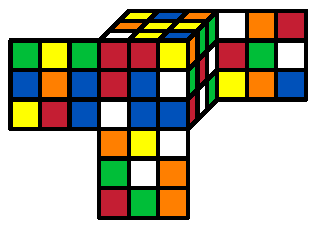
\includegraphics[width=5cm]{fig}\\
\caption{插图示例}
\end{figure}
\par
公式:正文中的公式、算式、方程式等必须编排序号,序号一律用阿拉伯数字分章依序编码,如:(3-32)、 (6-21)。
\par
对于较长的公式,另起行居中横排,只可在符号处(如:+、-、*、/、$<$$>$等)转行。公式序号标注于该式所在行(当有续行时,应标注于最后一行)的最右边。连续性的公式在“=”处排列整齐。大于999的整数或多于三位的小数,一律用半个阿拉伯数字符的小间隔分开;小于1的数应将0置于小数点之前。公式的行距一般为单倍行距。
\par
公式与正文之间一般应空一行。
\begin{equation}
\begin{split}
{X_{e1}}\left( {s,{n_1},{k_1}} \right) &= \left( {\begin{array}{*{20}{c}}
{{k_1}}\\
s
\end{array}} \right)\frac{{{n_1}!}}{{\left( {{n_1} - s} \right)!}}\sum\nolimits_{v = 0}^{\min \left( {{n_1} - s,{k_1} - s} \right)} {{{\left( { - 1} \right)}^v}\left( {\begin{array}{*{20}{c}}
{{k_1} - s}\\
v
\end{array}} \right)} \\
& \times \frac{{\left( {{n_1} - s} \right)!}}{{\left( {{n_1} - s - v} \right)!}}{\left( {{n_1} - s - v} \right)^{{k_1} - s - v}}
\end{split}
\end{equation}
\par
表:包括分类项目和数据,一般要求分类项目由左至右横排,数据从上到下竖列。
\par
分类项目横排中必须标明符号或单位,竖列的数据栏中不要出现“同上”、“同左”等词语,一律要填写具体的数字或文字。表序号一律用阿拉伯数字分章依序编码,如:表2.5、表10.3。
\par
每一个表格应有简短确切的题名,连同表序号置于表的正上方。表名称、表中的内容居中排列,字号为五号,中文字体为宋体,英文字体为Times New Roman,行距一般与正文保持一致。表格线统一用单线条,磅值为0.5磅。
\par
表格与正文之间一般应空一行。
\begin{table}
\renewcommand{\arraystretch}{1.5}
\caption{表格示例}
\label{tab0}
\centering
\begin{tabular}{|c|c|c|c|c|c|c|}
\hline
\multirow{2}{*}{\backslashbox{电性能参数}{馈电方式}}&\multirow{2}{*}{探针} & \multirow{2}{*}{环形缝隙}  & \multicolumn{2}{c|}{探针和缝隙} & \multicolumn{2}{c|}{缝隙和CPW} \\
\cline{4-7} & & &  探针 & 缝隙 & 缝隙 & CPW \\
\hline
谐振频率 & 9.5 GHz & 8.8 GHz & 9.4 GHz & 9.8 GHz & 9.2 GHz&9.3 GHz\\
\hline
\makecell[c]{带宽 \\ $|S_{11}|$ $<$-10 dB)}& 7.3\% & 4.5\% & 6.9\% & 6.8\% & 4.9\% & 5.3\% \\
\hline
\makecell[c]{隔离度\\(带内最差)} & -16.5 dB & -17 dB & \multicolumn{2}{c|}{-31 dB} & \multicolumn{2}{c|}{-22 dB} \\
\hline
方向图 & 不对称 & 对称 & 不对称 & 对称 & 对称 & 对称 \\
\hline
交叉极化电平 & 高 & 低 & 高 & 低 & 低 &低 \\
\hline
\end{tabular}
\end{table}
\par
计量单位:学位论文中出现的计量单位一律采用国务院1984年2月27日发布的《中华人民共和国法定计量单位》标准。

% \chapter{绪论}

\section{研究背景及意义}
自从我国80年代改革开放起,工业发展的速度就非常的迅速且稳定。
回顾近代工业史,我国在制造业方面的成就尤为亮眼,无论是工业化的科技理论水平还是实际成果产业都在世界舞台上有着令人瞩目的表现。
从官方数据总结中我们可以清晰的发现,在2017年我国GDP的构成中,有近乎三分之一的数据量来源自工业经济。从全球化的角度去对比,
通过当前世界工业标准分类我们可以清晰的发现,我国在22个总体大类中的煤炭,生铁等等七个传统大类中稳居制造生产的榜首,甚至在某些类别中具有压倒性地位;
同时针对于互联网时代下的新工业制造,我国也依旧具有很先进的科技手段和成熟的发展模式,
例如无论是工业机器人还是当今有着非常广泛应用的新能源汽车,我国都具有极高的市场占有率,并呈现出非常强劲的长期竞争力。
但是这并不代表着我国的工业发展是完美的,没有任何问题的。
我国工业前期的迅猛发展离不开人口红利和优势,仔细分析还会发现整体工业发展不平衡,
虽然科技理论非常先进,但是很多传统的工业流水线并不能利用被他们认为成“空中楼阁”的相关科学理论,
而是滞后的一直利用劳动力的廉价和数量的巨大进行重复的作业。这一现状随着整体人口结构的转型可预见的将会暴露越来越多的问题\cite{郭朝先2018改革开放40年中国工业发展主要成就与基本经验}。

传统的工业制造不再能满足21世纪以来新的产品需求:我们需要更加短的生产周期和更加复杂的产品性质,同时也不能忽略更加灵活的产品更新需求。
在这一现状的催生下,一个非常有创造性的理论被提出并逐渐完善应用。那就是柔性制造系统(Flexible Manufacturing System, FMS)。
这一系统着眼于现代工业对于多样和更新的需求,具有优秀的柔性化和智能化性质。
典型的FMS需要几个基本模块:数控机床,物料传递系统,计算机总控系统。
由于其集成性和网络化的特点,它为企业提供了更加高效、灵活的制造方式,从而提高了企业的竞争力。
较为典型的是它在生产时针对共享资源的处理,在实际工业生产中为相关的产线提供了极大的效率提升;
在无论是针对产品更新度还是多样化,柔性制造系统都为现代工业交出了一份令人惊艳的答卷\cite{李诚2015基于Petri网和启发式搜索的调度算法研究}\cite{金炳娥2010基于Petri网的柔性制造系统调度问题的研究}。
而在柔性制造系统中,有一个模块发挥着非常关键的作用,这一模块就是生产调度。这一模块的质量和效率直接关系到整体生产的质量和效率,无论从经济角度还是社会层面都具有非常战略性的意义。
但是这一问题经常是难以找到非常好的方式进行解决的:因为极其大量的实际产线调度问题都是多项式复杂程度的非确定性问题,
在学术界我们称之为NP(Non-deterministicPolynomial)完全问题\cite{李诚2015基于Petri网和启发式搜索的调度算法研究}\cite{李昭智1984NP-完全问题浅谈},
这一特点使得想要找到一个明确固定的规律是完全不可能的,从而导致了整体制造的调度非常的复杂。不止如此,随着工业发展,对于某些特定的产品,整体产线需要很多约束条件,
例如精确的时间要求,极端的生产环境等。这一实际情况无疑又加大了生产调度问题寻求更优方法的难度。综上我们不难发现,学术界和企业界都对调度问题有着非常大的关注度。

在新工业中,电子工业无疑是非常重要的一个方向。由于大多数电子组件的化学成分都为硅或部分含硅化合物,我们习惯性的直接将电子产业等同于半导体产业。
半导体产业与我们现代的生活息息相关,其中集成电路技术几乎出现在先进可以看到的所有电子产品中。
从大家每天使用的手机到机构企业需要的大型计算机,都不能离开集成电路,这也代表着半导体产业的强应用性。而在整体半导体产业中,对半导体的加工无疑是最具有经济效益和社会意义的产业。
具体对其进行分类,当今我国应用的主要技术包括晶圆制造加工,薄膜沉积、光刻、蚀刻、掺杂等等。
其中,晶圆制造这一步骤主要通过化学手段将硅精纯并制作成硅片达成;而晶圆加工往往需要更多的工业控制生产步骤加入,通过包括融化、晶体成长、裁切检测、切片清洗等等复杂而精确的加工步骤产生出最终的芯片。

想要解决晶圆制造问题,第一步就需要对一个现实复杂的模型进行精确又高效的建模。
只有数学模型贴合性好,我们才能正确的进行算法的模拟和运算,从而适应不同的加工需求和给出更优秀的调度结果。
一般在学术研究中,我们常用Petri网、自动机等对柔性制造系统进行建模分析;自动机无法很好的表述出系统并发关系,使针对晶圆制造这一典型的复杂离散系统,我们选择petri网进行建模\cite{顾佳颖2018考虑多重约束的半导体晶圆制造系统调度方法}\cite{贾林林2017半导体晶圆制造系统的瓶颈管理及调度优化研究}\cite{朱雪初,乔非2017基于工业大数据的晶圆制造系统加工周期预测方法}\cite{吴立辉,张洁2009基于多代理的知识有色赋时Petri网的晶圆制造系统建模方法}。

\section{国内外研究现状}
1962年,CarlAdam Petri在他的博士论文《与自动机通信》中首次提出了Petri网的概念。
后来,该模型被命名为Petri网,逐渐成为了理论计算机科学中的一个很有创造性的方向。
由于当时自动机理论中缺乏重要的并发概念,不适合描述和研究狭义相对论、测不准原理等现代物理学中的典型问题,
而Petri网模型能以自然、直观、易懂的方式分析并行系统的各种状态行为,这一非常优异的理论特色使得相关学术界中很多研究人员产生了浓厚的兴趣\cite{me2017}\cite{Martinez1986}。

1975年7月,麻省理工学院举办了第一届Petri网及相关理论研讨会。此后,国际上每年都会定期举办有关Petri网相关理论的研讨会,关于Petri网相关理论及其应用的研究成果不断涌现。
经过多年的深入研究,Petri网理论在垂直和水平两个方向上都得到了很大的发展和完善。
垂直发展体现在Petri网的建模理论上,从最基本的条件/事件网(C/E)、位置/过渡网(P/T)逐渐发展到谓词/过渡网和彩色网等高级网。
横向发展体现在Petri网的时间属性上,从非参数网发展到时间Petri网和随机Petri网。
目前,Petri网理论已广泛应用于柔性制造系统、离散事件系统、故障诊断系统、工作流建模与管理等多个领域\cite{5715371}\cite{vanderAalst2000}\cite{Clempner+2014+931+939}。

国内对于petri网的研究也在近30年中不断进步和完善。
1988年,南京航空航天大学的陈浩发表了第一篇关于Petri网的硕士论文,而随着国内学术界的不断耕耘和发展,相关的论文和成果达到近5000篇。
目前,仍有大量研究人员在该领域不断进行更深入的探索,相信未来会发现更多有用的研究成果。


\section{论文结构}
本文主要是研究基于Petri网和蚁群算法的柔性制造系统的调度问题,
基于库所时间网与变迁时间网提出一种新的时间网子类,
并使用此时间网子类对实际制造系统进行建模,
最后使用蚁群算法求解模型调度策略,
并结合模型实际情况,对蚁群算法设计了6种优化方案。
本论文包含五章,各章节主要内容如下:

第一章概括性地阐述了本文研究的背景与意义,简述了Petri网、各调度算法在国内外的现阶段的研究情况,然后总结了一系列求解调度问题的方法,最后给出了本文的组织结构。

第二章是本文的基础知识部分,这部分主要是详细介绍了Petri网的基本理论,包过Petri网的基本概念、定义和特性等,然后介绍了Petri网在晶圆制造领域的一些应用
并且介绍了基于Petri网的FMS建模相关理论与方法,通过一个简单的例子,简述了Petri网建模的过程。
最后介绍了一系列时间网。

第三章在第二章的基础上,将变迁时间网与库所时间网进行结合,提出变迁库所时间网这种新的时间网子类。
并基于变迁库所时间网设计了一种供调度算法使用的变迁发射流程,
并设计了一种用于计算各种Petri网模型调度策略的程序架构。
并通过一个简单的例子,描述了此发射流程的全过程。
在此基础上,使用变迁库所时间网对一个实际的晶圆制造系统进行建模。

第四章设计并使用蚁群算法对第四章建立的变迁库所时间网模型求解调度策略。
并对求解出的调度策略进行分析,对蚁群算法提出了一系列优化方案。
最后分别对这些优化方案进行实验分析。

最后一章为总结与展望,对本文所研究的内容进行了回顾,并提出了研究存在的不足以及接下来需要进一步研究的地方。
% \chapter{Petri网基本理论}
本章为本文的理论研究的基础,主要介绍了Petri网概念与特性,包过:Petri网定义、Petri网模型结构、Petri网可达图和Petri网特性;
介绍了Petri网在不同领域的应用;
介绍了一系列Petri网的调度方法;
最后介绍了一系列时间网。
为后续章节提供理论支持。
\section{Petri网概念与特性}
    Petri网是一种描述离散事件系统的数学模型,它既可以用数学定义形式化地表示,也可以用图形形象化地表示。
    使用Petri网建立的模型具有简单、易懂、可操作性强等特点,能够很直观地表述出各类实际系统模型中并发、依赖、冲突、死锁等情况。
    Petri网既可用于结构分析又可用于行为分析,因此在各个领域均有广泛应用\cite{24143}\cite{7426418}\cite{wu:hal-00735482}。

    \subsection{Petri网定义}
    一个Petri网中通常是由两种节点组成的图,这两种节点分别为:库所(Place),变迁(Transition),
    每个元素含义与功能各不相同:库所中存放托肯(Token),托肯表示系统的资源;
    变迁一般代表能够改变系统状态的某种事件,变迁执行一种称为发射的操作,变迁发射后会改变库所中的资源的状态,从而改变系统的状态;
    变迁和库所间通过有向弧(Arc)连接,如果有向弧从库所指向变迁,意味着变迁发射后会从库所中取走一定数目的托肯,如果有向弧从变迁指向库所,意味着变迁发射后会放入一定数目的托肯进库所;
    Petri网也可以图形表示,
    在图形上分别用矩形($\Box $)表示变迁、圆圈($\bigcirc $)表示库所,某些变迁和托肯间会通过箭头连接,箭头($\leftarrow$)表示有向弧。

    \textbf{定义2.1}\cite{murata1989petri}\textbf{:}
    Petri网可以用一个四元组进行数学表示,四元组的元素分别为:库所集合、变迁集合、有向弧集合、有向弧上到权值的映射关系,即$N=(P,T,F,W)$,
    $P=\{p_{0},p_{1},p_{2},...,p_{i}\}$,$i \in \mathbb{N}^{+}$,是一个限非空的库所集合;
    $T=\{t_{0},t_{1},t_{2},...,t_{j}\}$,$j \in \mathbb{N}^{+}$,也是一个限非空的变迁集合;
    这两个集合不存在相交部分,因为Petri网中的一个元素不能即是库所又是变迁,即$P \neq \emptyset , T \neq \emptyset, P \cap T=\emptyset$。
    库所和变迁间通过有向弧连接,即
    $F \subseteq(P \times T) \cup(T \times P)$。
    弧上带有权值,即i
    $W:(P \times T) \cup(T \times P) \rightarrow \mathbb{N}$,对于任意$w \in W$,$w=1$,如果存在某个权值$w$不为1,则称这个网为一般网。
i
    \textbf{例2.1}\hspace{0.5em}
    如图2.1就是某Petri网的图形表示,他的数学表示为:$N = (P, T, F, W)$,$P =  \{p_{1}, p_{2}, p_{3}, p_{4}, p_{5}, p_{6}\}$为此Petri网库所的集合,
    此Petri网有6个库所;
    $T = \{t_{1}, t_{2}, t_{j3}, t_{4}\}$ 为此Petri网变迁的集合,
    此Petri网有4个变迁;
    \begin{equation}
        \begin{aligned}
            F = \{(p_{1}, t_{2}), (t_{1}, p_{1}), (p_{2}, t_{3}), (t_{2}, p_{2}), (p_{3}, t_{4}), \\(t_{3}, p_{3}), (p_{4},t_{1} ), (t_{2},p_{4} ), (p_{5}, t_{3}), (t_{4}, p_{5}), (p_{6}, t_{1}), (t_{4}, p_{6})\}
        \end{aligned}
        \nonumber 
    \end{equation}为此Petri网有向弧集合,
    有向弧的权值为:$W(p_{1}, t_{2}) = W(t_{1}, p_{1}) = W(p_{2}, t_{3}) = W(t_{2}, p_{2}) = W(p_{3}, t_{4}) = W(t_{3}, p_{3}) = W(p_{4},t_{1}) = W(t_{2},p_{4} ) = W(p_{5}, t_{3} ) = W(t_{4}, p_{5} ) = 1$,
    $W(t_{4}, p_{6})=W(p_{6}, t_{1}) = 2$。
    因为这个网中的有向弧上的权值并不全为1,而是存在2个有向弧上权值为2,所以是一个一般网。
    
    \begin{figure}[H]
        \centering
        % Requires \usepackage{graphicx}
        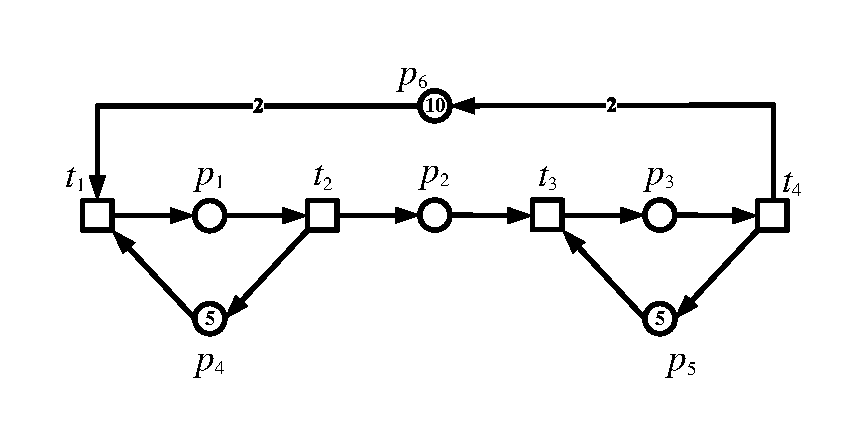
\includegraphics[scale=0.8,angle=0]{figures/figure2-1.pdf}\\
        \caption{一个一般Petri网模型}
    \end{figure}

    \textbf{定义2.2}\cite{Liu2013}\textbf{:}
    对于某Petri网$N = (P, T, F, W)$,在此网中的任意一个节点$m \in P \cup T$,分别在其前后打点,表示此节点的前置节点集合和后置节点集合,
    记$^{\bullet}m$为节点$m$的前置集合,$^{\bullet} m = \{n \in P \cup T|(n, m) \in F\}$;
    记$m^{\bullet}$为节点$m$的后置集合,$m^{\bullet} = \{n \in P \cup T|(m, n) \in F\}$,
    如果节点$m \in P$,那么$^{\bullet}m \subseteq T$,$m^{\bullet} \subseteq T$,
    如果节点$m \in T$,那么$^{\bullet}m \subseteq P$,$m^{\bullet} \subseteq P$,
    相应地,将全部节点的集合记作$M \subseteq (P \cup T)$,则节点集合满足$^{\bullet}M = \cup _{m \in M} {^\bullet}m$,$M^{\bullet} = \cup_{m \in M} m^{\bullet}$。
    若满足$\forall i\in \mathbb{N}^+ = \{1, 2,...,n-1\}$,$y_{i+1} \in y_i^{\bullet}$。 此节点序列$m_{1}, m_{2},..., m_{i},...,m_{j}$ 即为Petri网$N$的路径,其中$m_{i} \in P \cup T$。
    如果在这条路径中除了$m_{1}$和$m_{j}$以外,所有的节点都不相同,并且$m_{1} = m_{j}$,即此节点序列的首尾相同,遍历此序列最终会回到原点,因此此序列构成一条回路,此Petri网被称为一条简单回路。
    
    在定义2.2中,
    如果$m$表示库所,此库所的前置集$^{\bullet} m$中的变迁称为输入变迁,
    此库所的后置集$m^{\bullet}$中的变迁称为输出变迁集。
    如果$m$表示变迁,此变迁的前置集$^{\bullet} m$中的库所称为输入库所,
    此变迁的后置集$^{\bullet} m$中的库所称为输出库所。

    \textbf{例2.2}\hspace{0.5em}
    如图2.2所示,是一个简单的Petri网模型,此网P中所有库所($p_{1},p_{2},p_{3},p_{4},p_{5}$) \\ 的前置变迁集合与后置变迁集合为:
    $^\bullet p_1 = \{t_1\}$,${p_1}^\bullet = \{t_2\}$,
    $^\bullet p_2 = \{t_2\}$,${p_2}^\bullet = \{t_3\}$,
    $^\bullet p_3 = \{t_3\}$,${p_3}^\bullet = \{t_4\}$,
    $^\bullet p_4 = \{t_2, t_4\}$,${p_4}^\bullet = \{t_1, t_3\}$,
    $^\bullet p_5 = \{t_4\}$,${p_5}^\bullet = \{t_1\}$。
    网模型中所有变迁($t_{1},t_{2},t_{3},t_{4}$)的前置库所集合和后置库所集合为:
    $^\bullet t_1 = \{p_4, p_5\}$,${t_1}^\bullet = \{p_1\}$,
    $^\bullet t_2 = \{p_1\}$,${t_2}^\bullet = \{p_2, p_4\}$,
    $^\bullet t_3 = \{p_2, p_4\}$,${t_3}^\bullet = \{p_3\}$,
    $^\bullet t_4 = \{p_3\}$,${t_4}^\bullet = \{p_4, p_5\}$。
    对于一组节点序列:$p_1, t_2, p_2, t_3, p_3, t_4, p_4, t_1, p_1$就是此Petri网的一条路径,因为此路径的首尾相同,其他节点均不相同,因此这是一条简单回路。
    
    \begin{figure}[H]
        \centering
        % Requires \usepackage{graphicx}
        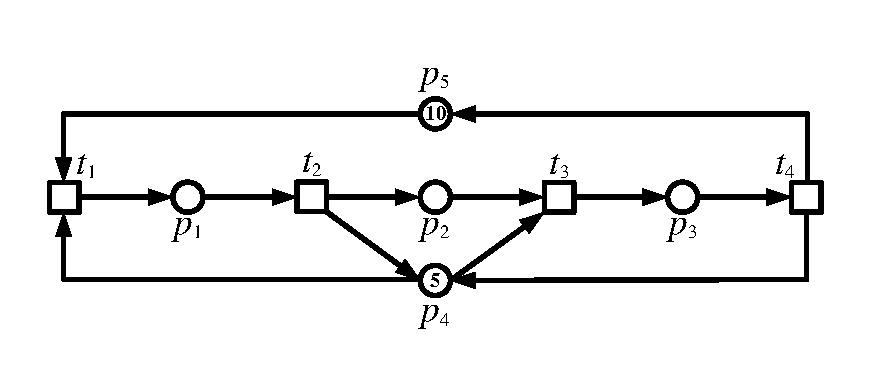
\includegraphics[scale=0.8,angle=0]{figures/figure2-2.pdf}\\
        \caption{一个Petri网模型}
    \end{figure}

    \textbf{定义2.3}\cite{murata1989petri}\textbf{:}
    一个Petri网$N = (P, T, F, W)$,如果满足条件$\forall x, y \in (P \cup T)$,$W(x, y)> 0$,$W(y, x) = 0$,则将此Petri网称为一个纯网(pure net)。
    
    要判断一个Petri网是否是纯网,可以使用关联矩阵,以及前置矩阵和后置矩阵。$[N]$是$|P| \times |T|$的一个整数矩阵。$[N]$可以进一步进行拆分为$[N]^+$和$[N]^-$ ,对其进行矩阵运算得到$[N]$,运算公式为$[N]=[N]^+ - [N]^- $。其中$\forall t \in T$,$\forall p \in P$,$[N]^+(p,t) = W(t, p)$,$[N]^-(p,t) = W(p, t)$。
    
    \textbf{例2.3}\hspace{0.5em}
    图2.2所示的Petri网模型,所有的有向弧只有一个方向,因此此Petri网没有自环,是一个纯网。

    对于图2.2中所示的Petri网中,将其库所变迁的关系分解为如下三个矩阵,其中$[N]^+$为输入关联矩阵,$[N]^-$为输出关联矩阵,$[N]$为关联矩阵。
    \begin{equation}\label{equaN}
    [N^+]=\begin{pmatrix}
    0&1&0&0\\
    0&0&1&0\\
    0&0&0&1\\
    1&0&1&0\\
    1&0&0&0
    \end{pmatrix}\ \ \ \ \ \ \
    [N^-]=\begin{pmatrix}
    1&0&0&0\\
    0&1&0&0\\
    0&0&1&0\\
    0&1&0&1\\
    0&0&0&1
    \end{pmatrix}\ \ \ \ \ \ \
    [N]=\begin{pmatrix}
    -1&1&0&0\\
    0& -1&1&0\\
    0 &0&-1&1\\
    1&-1 &1&-1\\
    1&0&0&-1
    \end{pmatrix}
    \end{equation}

    在上述所示的关联矩阵中,$[N^+]_{(p_1,t_2)}=1$,意味这如果此Petri网发射$t_2$变迁,会往库所$p_1$中放入1个托肯,
    $[N^-]_{(p_1,t_2)}=0$,意味着发射$t_2$变迁,不会往$p_1$取走托肯,
    前两个关联矩阵复合后得到的$[N](p_1,t_2)=1$意味着如果此Petri网发射$t_2$变迁,库所$p_1$中的托肯数量会加1。

    \textbf{定义2.4}\cite{Liu2010}\textbf{:}
    Petri网$N = (P,T,F,W)$中任意标识$M$都是一个维数与库所数相同的自然数向量。$(P,T,F,W,M_{0})$也可以直接记为$(N,M_{0})$,$N$表示Petri网的结构,$M_{0}$称为网系统的初始标识,表示Petri网的初始状态。

    \textbf{例2.4}\hspace{0.5em} 图2.2所示的Petri网,此Petri网的初始标识向量为:$M_{0}=(0,0,0,5,10)^{T}$,
    也可以使用与库所有关的多项式表示,
    即当表示向量对应库所的数值作为系数,乘上对应库所,再求和组成的多项式
    对于初始标识$M_{0}$,此标识向量为:
    $M_{0}=5p_{4}+10p_{5}$。

    \textbf{定义2.5}\cite{Liu2013}\textbf{:}
    对于某Petri网,如果在当前标识$M$下,如果某个变迁$t$满足$\forall p\in{^\bullet t}, M(p) \geq W(p,t)$,
    则称变迁$t$在标识$M$下是使能的,并将其记作$M[t\rangle$。一般来说,Petri网库所是有容量限制的,如果变迁$t$ 在标识$M$下是使能的,并且变迁$t$发射后,不会超过库所容量的限制,即满足$\forall p \in t^{\bullet}, M(p)+W(t,p) \leq MAX(p)$,
    则此变迁能被安全发射,其中$MAX(p)$表示库所$p$中能够存放的最多托肯的数量,也就是库所容量。变迁$t$ 发射后会改变Petri网模型中各库所中托肯的状态,因此Petri网的状态也就被改变了,从而产生一个新的Petri网的标识,在可达图中新标识是原标识的后继节点,两标识通过变迁连接,新标识的计算公式为$M^{\prime}(p)=M(p)-W(p,t)+W(t,p)$,
    原标识与新标识的关系记为$M[t\rangle M^{\prime}$,表示可达状态$M$可以通过发射变迁$t$到达可达状态$M^{\prime}$。

    \textbf{例2.5}\hspace{0.5em}
    在图2.2所示的Petri网模型中,初始标识为$M_{0}=5p_{4}+10p_{5}$,表示库所$p_{4}$中有5个托肯,库所$p_{5}$中有10个托肯,在此标识下变迁$t_1$是可以安全发射的,
    记作$M_0 [t_1\rangle$,表示变迁$t_1$在状态$M_{0}$下发射后既不会使库所中的托肯数为负数,也不会超过库所容量。
    变迁$t_1$的前置库所集合为$^\bullet t_1 = \{p_4, p_5\}$,分别判定$p_4$,$p_5$两个库所是否能安全地取走托肯:$M_0(p_4)=5 > W(p_4, t_1)=1$,$M_0(p_5)=10 > W(p_5, t_1)=1$,这两个库所中都有足够多的托肯数发射变迁$t_1$,所以变迁$t_1$能够发射,
    在发射后,库所$p_1$的托肯数更新为$M_1(p_1)=M_0(p_1)-W(p_1, t_1)+W(t_1, p_1)=1$,
    库所$p_4$的托肯数更新为$M_1(p_4)=M_0(p_4)-W(p_4, t_1)+W(t_1, p_4)=4$, 
    库所$p_5$的托肯数更新为$M_1(p_5)=M_0(p_5)-W(p_5, t_1)+W(t_1, p_5)=9$。
    此Petri网的标识从$M_0=5p_4+10p_5$更新为$M_1=p_1+4p_4+9p_5$,
    $M_0$可以通过发射$t_1$到达$M_1$,记作$M_0[t_1\rangle M_1$。

    \textbf{定义2.6}\cite{Liu2013}\textbf{:}
    如果对于Petri网$N$,初始标识$M$发射某变迁后能够到达新标识$M^{\prime}$,
    则称$M$到$M^{\prime}$是可达的,记为$M[\delta\rangle M_{n}$,
    如果$M[t_{1}\rangle M_{1}[t_{2}\rangle M_{2}\ldots M_{n-1}[t_{n}\rangle M_{n}$,
    意味着$t_1$,$t_2$可以被连续发射,
    则变迁序列$\delta=t_{1}t_{2}\dots t_{n-1}t_{n}$ 为网中的一个可发射的序列,
    $M_{1},M_{2},\dots,M_{n-1},M_{n}$为Petri网$N$的可达标识。
    因为这两个变迁均可发射,所以可以使用下述状态方程直接计算发射这两个变迁后的标识,
    $M_{n}=M+[N]\overrightarrow{\delta}$,其中将$\overrightarrow{\delta}$: $T\rightarrow \mathbb{N}$称作是计数型整数向量,在发射序列$\delta$中变迁$t$发射的次数和可以用$\overrightarrow{\delta}(t)$来表示。

    \textbf{例2.6}\hspace{0.5em}
    如图2.2所示,在此Petri网$N$中发射一条变迁序列$\delta=t_1t_2t_3t_4$,其中$\overrightarrow{\delta}= [1 \quad 1 \quad 1 \quad 1]^T$称为Petri网$N$的发射向量。
    通过发射变迁序列$\delta$产生了新的可达标识$M'$ ,此过程可以使用下述状态方程表示:
    
    \begin{equation}\label{equaM}
    M_n=M_0+[N]\overrightarrow{\delta}=\begin{pmatrix}
    0\\
    0\\
    0\\
    5\\
    10
    \end{pmatrix}+\begin{pmatrix}
    -1&1&0&0\\
    0& -1&1&0\\
    0 &0&-1&1\\
    1&-1 &1&-1\\
    1&0&0&-1
    \end{pmatrix}\begin{pmatrix}
    1\\
    1\\
    1\\
    1
    \end{pmatrix}=
    \begin{pmatrix}
    0\\
    0\\
    0\\
    5\\
    10
    \end{pmatrix}=M_0
    \end{equation}
    
    此变迁序列发射完后,又回到了初始标识$M_0$,这是因为这个发射序列正好是此Petri网的一条完整的回路,并且所有的弧上权值均为1。

    \textbf{定义2.7}\cite{murata1989petri}\textbf{:}
    对于一个Petri网$N$,从某标识$M$出发,能够通过变迁序列到达的所有标识的集合记为$M[\rangle$。
    如果是从初始标识$M_{0}$出发,其可达标识集为$M_{0}[\rangle$,也可以记为$R(N,M_{0})$。
    在标识$M_{0}$下,如果$\exists M^{\prime}\in R(N,M)$ 使得$M^{\prime}[t\rangle$,
    当且仅当对$\forall M \in R(N,M_{0})$成立;
    对于变迁集中的所有变迁,即$\forall t \in T$,
    则变迁$t$是活的,如果存在某变迁在初始标识$M_0$下是活的,
    则网$(N,M_{0})$是活的(live);
    对于初始标识下所有的可达标识$\forall M \in R(N,M_{0})$,
    如果$\nexists t \in T$ ,$M^{\prime}[t\rangle$ ,
    则此Petri网$(N,M_{0})$是无死锁的(deadlock-free)。

    \textbf{例2.7}\hspace{0.5em}
    判定2.3所示的三个Petri网的活性。

    \begin{figure}[H]
        \centering
        % Requires \usepackage{graphicx}
        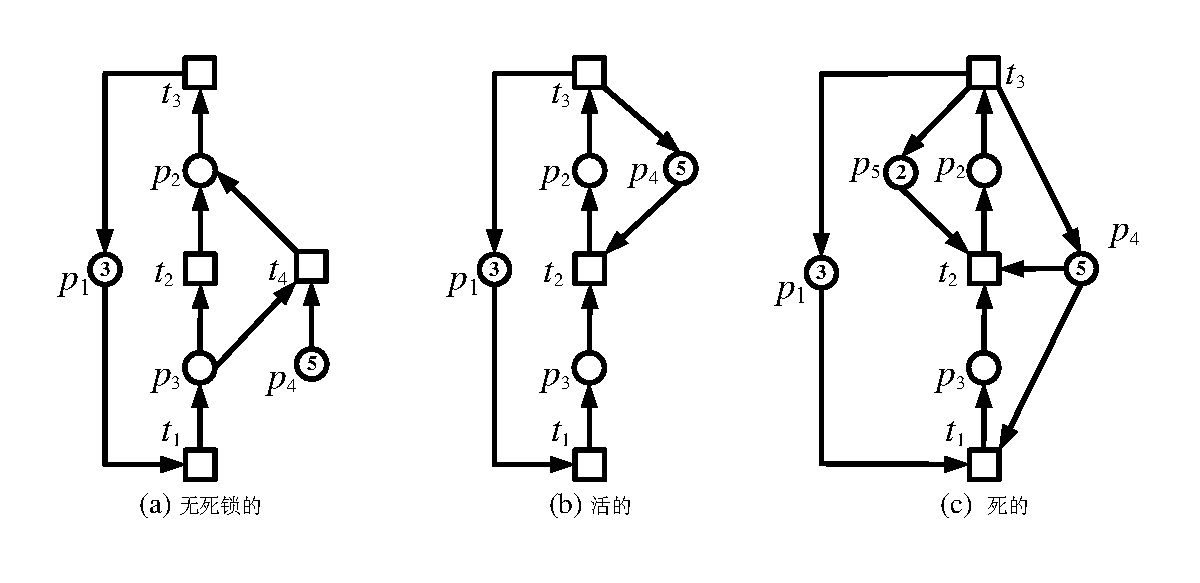
\includegraphics[scale=0.7,angle=0]{figures/figure2-3.pdf}\\
        \caption{一个Petri网活性示例}
    \end{figure}

    图2.3(a)中的Petri网没有死锁标识,变迁变迁$t_{4}$不是活的,因此称此Petri网是无死锁的;
    图2.3(b)中的Petri网所有变迁都是活的,因此称此Petri网活的;
    图2.3(c)中的Petri网存在死锁标识,因此称此Petri网是死的。
    \subsection{Petri网模型结构}
    使用Petri网建模,可以很直观地描述出模型结构\cite{petri},本小节将对Petri网中的四种结构模型:顺序、并发、冲突、混淆进行详细介绍。
    \subsubsection{顺序关系}
    在某标识下,如果某变迁发射,可以时原本不能使能的变迁使能,也就是说变迁可以顺序发射下去,则称这两个变迁在这个标识下是顺序关系,如图2.4(a)所示。

    \textbf{定义2.8}\cite{petri}\textbf{:}
    对于标识$M$,$\exists $变迁$t_{1}$、$t_{2}$,$M[t_1\rangle M'$,$\lnot M[t_2\rangle$,$M'[t_2\rangle$,
    变迁$t_{1}$、$t_{2}$在标识$M$下为顺序关系。
    \subsubsection{并发关系}
    在某标识下,如果两个变迁都可以使能,并且其中任何一个变迁发射都不会使另一个变迁不使能,就称这两个变迁为并发关系。并发关系下的两个变迁,是可以独立发射的,如图2.4(b)所示。

    \textbf{定义2.9}\cite{petri}\textbf{:}
    对于标识$M$,$\exists $变迁$t_{1}$、$t_{2}$,$M[t_1\rangle$,$M[t_2\rangle$,并且$M[t_1\rangle M_1\Rightarrow M_1[t_2\rangle$,$M[t_2\rangle M_2\Rightarrow M_2[t_1\rangle$,
    变迁$t_{1}$、$t_{2}$在标识$M$下为并发关系。
    \subsubsection{冲突关系}
    与并发关系正好相反,如果在某标识下,两个使能变迁发射任何一个,都会使另一个无法使能,则称这两个变迁在这个标识下是冲突关系,如图2.4(c)所示。

    \textbf{定义2.10}\cite{petri}\textbf{:}
    对于标识$M$,$\exists $变迁$t_{1}$、$t_{2}$,$M[t_1\rangle$,$M[t_2\rangle$,并且$M[t_1\rangle M_1\Rightarrow M_1[t_2\rangle$,$M[t_2\rangle M_2\Rightarrow M_2[t_1\rangle$,
    变迁$t_{1}$、$t_{2}$在标识$M$下为并发关系。
    \subsubsection{混淆关系}
    如果一个Petri网中同时存在并发和冲突两种关系的变迁,并且并发关系的变迁发射后会时冲突关系消失。在这种情况下是无法判断出冲突关系是否出现过的,因此称变迁间的这个关系为混淆关系,如图2.4(d)所示。

    \begin{figure}[H]
        \centering
        % Requires \usepackage{graphicx}
        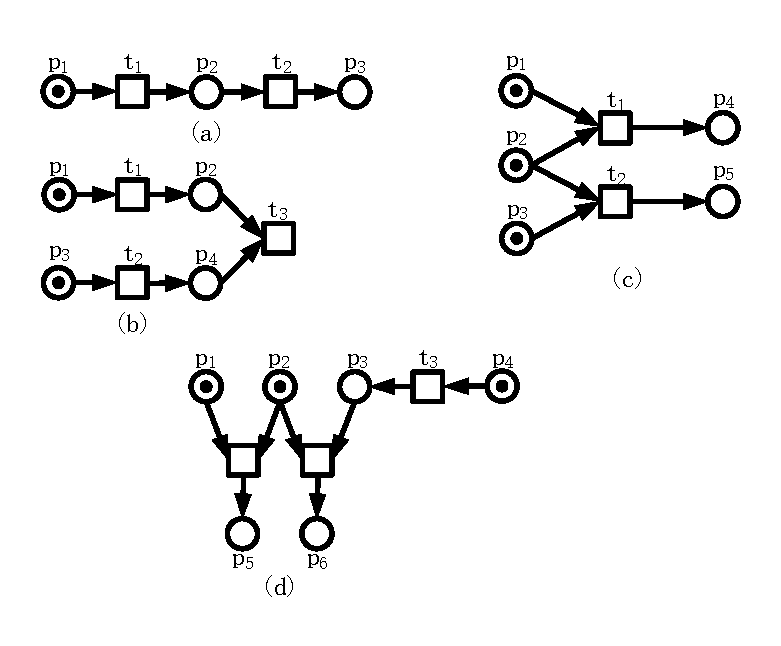
\includegraphics[scale=0.7,angle=0]{figures/figure2-4.pdf}\\
        \caption{Petri网模型结构}
    \end{figure}

    \subsection{Petri网可达图}
    本文所研究的调度算法需要在Petri网可达图中搜索一条路径,所以本节将要介绍Petri网可达图(reachability graph)。
    可达图是分析Petri网的重要工具,而且不论是何种Petri网都有可达图。在可达图中可以清晰直观地看出不同标识是如何通过变迁转换的。
    给出Petri网以及此Petri网的初始标识,便可确定这个Petri网的可达图。
    利用Petri网可达图可以分析此Petri网所描述的离散事件系统的可达性、有界性、活性、安全性等一些列重要性质,是Petri网理论中十分有用的分析工具。

    \textbf{定义2.11}\cite{li2009deadlock}\textbf{:}
    记一个Petri网$(N, M_{0})$的可达图为$RG(N, M_{0})= (U, S)$,可达图中包含该网模型的所有可达标识以及可达标识之间的变迁关系,可达图是一个有向图。
    其中,可达图中用圆圈表示节点,
    用$U= R(N, M_{0})$代表网的全部可达标识;可达图中节点之间的有向连接弧用集合$S= \{(M, t, M^{\prime})\mid M^{\prime} \in R(N, M_{0})$,$M[t\rangle M^{\prime}\}$来表示,
    弧上标注了对应的变迁,用来说明从一个可达标识到达另一个可达标识所需要发射的变迁,也就是可达标识之间的映射关系。

    可达图算法与传统的图遍历算法并无本质上的区别。
    通过算法2.1\cite{zby2019}可以得到一个Petri网的可达图:

    \begin{algorithm}[H]
        \caption{可达图算法}
        \label{alg2-1}
        \begin{algorithmic}
            \Procedure {RG}{}
            \Require 一个标记的Petri网 $(N, M_{0})$。 \notag
            \Ensure 网模型的可达图。
            \State 可达图$RG(N,M_{0})$的开始点为初始标识$M_{0}$
            \State 一开始Petri网的全部可达标识没有被标记
            \State \textbf{while}\{有可达标识未被标记\}\textbf{do}
                
                \State \hspace{0.8cm} 对未被标记的可达标识$M$
                
                \State \hspace{0.8cm} 考虑可达标识$M$下每一个使能的变迁$t$,通过$M^{\prime}=M+[N](\cdot,t)$计算新的可达标识$M^{\prime}$
                
                \State  \hspace{0.8cm} \textbf{if}\{可达图$RG$中还没有添加新的可达标识$M^{\prime}$\} \textbf{then}
                
                \State \hspace{1.4cm}  将新的可达标识$M^{\prime}$添加到可达图中
                
                \State \hspace{1.4cm}  在$M$到$M^{\prime}$之间添加有向弧并标记为$t$
                
                \State \hspace{0.8cm} \textbf{end if}
                
                \State  \hspace{0.8cm} 标记可达标识$M$
                
            \State  \textbf{end while}
            \EndProcedure
        \end{algorithmic}
    \end{algorithm}

    对图2.2中的Petri网使用此算法求取可达图,为了减少可达标识数,将初始标识改为$(0,0,0,1,2)$,将得到如下可达标识:

    \begin{table}[H]
        \centering
        \begin{tabular}{|l|l|}
        \hline
            可达标识 & 使能变迁 \\ \hline
            $M_0:(0,0,0,1,2)$ & $t_1$ \\ \hline
            $M_1:(1,0,0,0,1)$ & $t_2$ \\ \hline
            $M_2:(0,0,1,0,1)$ & $t_4$ \\ \hline
            $M_3:(0,2,0,1,0)$ & $t_3$ \\ \hline
            $M_4:(0,1,1,0,0)$ & $t_4$ \\ \hline
            $M_5:(0,1,0,1,1)$ & $t_1$ $t_3$ \\ \hline
            $M_6:(1,1,0,0,0)$ & $t_2$ \\ \hline
        \end{tabular}
        \caption{图2.2中的Petri网可达图}
    \end{table}

    \subsection{Petri网特性}
    Petri网的特性包过可达性、有界性、活性、可逆性、可覆盖性和持续性\cite{jcj2003},可使用上一节提到的可达图分析Petri网的这些特性。
    本节将简略介绍上述特性的含义。
    \subsubsection{可达性}
    可达性将是本文调度算法部分最为关注的特性。如果存在某条变迁序列$\delta $,使得初始标识$M_0$按此变迁序列发射,能够到达标识$M'$,就说$M'$是从$M_0$可达的,记作$M_0[\delta\rangle M'$。
    如果$\delta $中只有一个变迁,则说$M'$是从$M_0$立即可达的。
    实际上调度算法所要做的就是找到一条最优的变迁序列。
    一个Petri网$N$的所有可达标识组成一个可达标识集,记作$R(N,M_0)$或$R(M_0)$。
    表2.1就是图2.2中的Petri网的可达标识集,这里面所有标识都是可达的。
    \subsubsection{有界性}
    有界指的是Petri网的可达标识数是有限的,也可以描述成Petri网从初始标识$M_0$开始任何一个可达标识中任意一个库所的托肯数都有界。
    实际的物理模型中许多是有界的,一般情况下库所指的是存放资源的场所,是有容量的。
    实际建模时一般会直接给出库所容量的约束。
    表2.1中只有7个可达标识,因此图2.2中的Petri网是有界的。
    \subsubsection{活性}
    Petri网的活性和Petri网中是否有死锁有相关性。如果可达图的任何子图中都存在一个标识能使变迁$t$使能,则说明变迁$t$是活的,如果所有变迁都是活的,则称Petri网是活的。
    如果Petri网是活的,则它一定没有死锁标识。
    图2.2中的Petri网就是活的。
    \subsubsection{可逆性}
    可逆性也和Petri网中是否有死锁有相关性。如果可达图中任意一个可达标识都可以通过发射某条变迁序列回到初始标识,则称Petri是可逆的。
    因此如果Petri网是可逆的,则它一定没有死锁标识。
    图2.2中的Petri网就是可逆的。
    \subsubsection{可覆盖性}
    对于标识$M$,如果Petri网可达图中存在标识$M'$,$M'$中每个库所的托肯数都比$M$的大,则说明$M$是可覆盖的。
    \subsubsection{持续性}
    具有持续性的Petri网,一旦某变迁使能了,那它会一直使能,直到发射此变迁为止。
    图2.2中的Petri网的$t_2$、$t_3$、$t_4$变迁都是可持续的。
\section{Petri网的应用}
    在解决柔性制造系统生成调度问题时,Petri网能够充分反应实际模型的各种特性,因此Petri网在此方面应用十分广泛。Petri网在柔性制造系统中的各种应用如图2.5所示。
    \begin{figure}[H]
        \centering
        % Requires \usepackage{graphicx}
        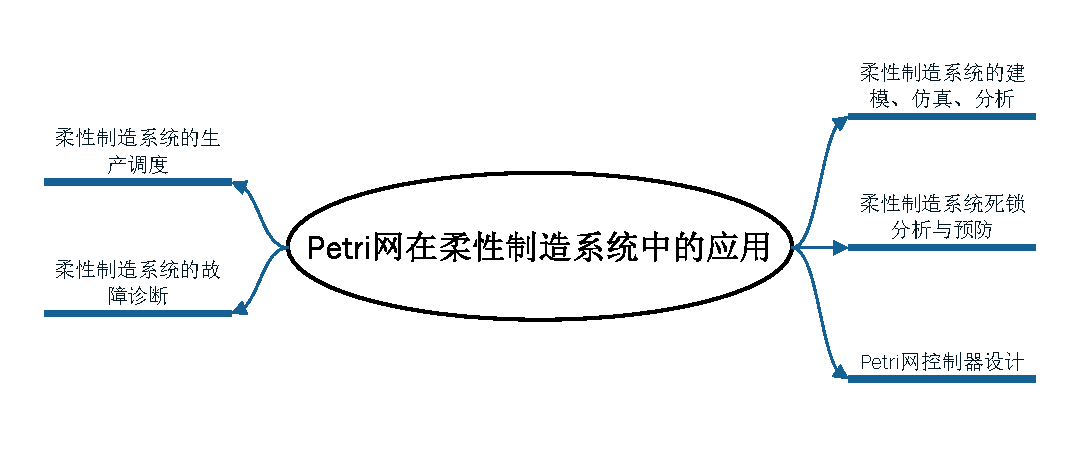
\includegraphics[scale=0.7,angle=0]{figures/figure2-5.pdf}\\
        \caption{Petri网在柔性制造系统中的各种应用}
    \end{figure}
\section{Petri网的调度方法}
    本文将着重研究基于蚁群算法的Petri网调度问题。这是一个群体智能的图搜索算法,在Petri网背景下,搜索的空间是可达图。
    因此本节将对各种图搜索算法进行介绍。
    本节介绍的算法分为两个大类:传统的图搜索算法、群体智能算法。
    \subsection{传统的图搜索算法}
        传统的图搜索算法具有很相似的结构。本类算法有两个集合,一个集合用于存放待扩展的节点,另一个集合用于存放已经扩展过的节点。
        每次从待扩展的节点集合中取出节点,基于此扩展新节点,如果新节点不在存放已经扩展过的节点集合中存在,则说明它有扩展的价值,将其放入待扩展的节点集合中。
        不断重复上述操作,直到找到终点,或者待扩展的节点集合为空。
        \begin{algorithm}[H]
            \caption{图搜索算法}
            \label{alg2-2}
            \begin{algorithmic}
                \Procedure {graphSearch}{}
                    \State 将起点存入待扩展的节点集合
                    \While{待扩展的节点集合不为空}
                        \State $curr \leftarrow$ 从待扩展的节点集合取出节点
                        \While{$curr$未完成扩展}
                            \State $next \leftarrow$ 扩展一个$curr$的后继节点
                            \If{$next$不在存放已经扩展过的节点集合中存在}
                                \State 将$next$放入待扩展的节点集合中
                            \EndIf
                        \EndWhile
                        \State 将$curr$放入已经扩展过的节点集合中
                    \EndWhile
                \EndProcedure
            \end{algorithmic}
        \end{algorithm}
        此后的一系列算法都是对从待扩展的节点集合取出节点这一步进行更精细的设计,从而改变图搜索的顺序。
        \subsubsection{深度优先搜索}
        深度优先搜索算法如果不发生回溯,每次扩展的节点都是相邻的,这意味着当前节点完成扩展后必须从它扩展出的新节点选择下一次要扩展的节点。
        因此因该选择先入后出的堆栈来实现待扩展的节点集合\cite{chen2019depth}\cite{liu2018improved}\cite{wu2017depth}\cite{zhang2016novel}\cite{chen2015improved}。
        \subsubsection{基于Petri网的启发式调度}
        此算法是深度优先搜索算法的一个子类,通过设计对当前节点更为精细的扩展顺序来实现。
        比如每次都以单步最优的策略进行扩展,则可将当前节点的后继节点按距离排序后放入待扩展的节点集合中。
        体现在Petri网中,即为每次都发生最短完工的变迁,此策略称为最早完工策略\cite{johnson1954optimal}\cite{wagner1959theory}\cite{winston1969production}\cite{mather1972production}\cite{graves1981production}。
        \subsubsection{广度优先搜索}
        广度优先搜索会一层层地扩展搜索树,因此需要按顺序依次扩展当前节点的后继节点。
        因此待扩展的节点集合应选取先进后出的队列进行实现\cite{cormen2009introduction}\cite{yang2019approximating}\cite{liu2015new}\cite{mehlhorn1999data}\cite{yu2015research}。
        \subsubsection{迪杰斯特拉算法}
        迪杰斯特拉算法与广度优先搜索算法类似,在大方向上也是一层层地扩展可达树。
        不同的是,迪杰斯特拉算法每次扩展的节点都是待扩展的节点集合中离原点距离最短的。
        因此迪杰斯特拉算法一定能求出全局的最短路径\cite{dijkstra1959note}\cite{cormen2009introduction}\cite{sedgewick1990algorithms}\cite{dijkstra1976discipline}\cite{brandes2005centrality}。
        \subsubsection{启发式搜索算法}
        此算法又称A星算法,是对迪杰斯特拉算法的进一步优化。
        此算法的待扩展的节点集合会对每一个进入集合的节点进行估计,
        估计的是经过此节点的最短路径的长度。
        此长度值$f$分为两部分:起点到当前点的最短路径长度$g$、当前节点到终点的最短路径长度$h$,
        $$
            f=g+h
        $$
        如果估计合理,$g$的值是确定的,因为每次扩展都会往最优解上走,$g$的值就是当前路径当前节点离原点的距离。
        因此$h$的值将是影响算法的关键。

        因为Petri网的启发式函数需要结合具体情况进行设计,而本文研究的蚁群算法是一种通用的图搜索算法,所以本文在算法章节并不对A星算法进行测试。
        而深度优先搜索和广度优先搜索策略太过简单,效果是不如其他更为精细的搜索机制的,因此本文将主要使用Petri网的启发式调度、迪杰斯特拉算法为传统搜索算法的代表进行测试\cite{hart1968formal}\cite{russell2010artificial}\cite{nash2011incremental}\cite{sturtevant2012benchmarks}\cite{botea2004near}。
    \subsection{群体智能算法}
        群体智能算法之间流程差异巨大,但本质思想是类似的。
        群体智能算法会并发地开启多条搜索路径,并提供某种正反馈机制把解往优的解上引导。
        \subsubsection{遗传算法}
            遗传算法大体流程为:

            1、将问题的解编码为染色体;

            2、对一系列染色体评价其适应度;

            3、按适应度大小淘汰一批染色体;

            4、从幸存的染色体中使用交叉操作生成新的染色体;

            5、重复进行上述操作一定轮次后对适应度最高的染色体进行解码,得到并输出解\cite{eiben2015evolutionary}\cite{whitley1994genetic}\cite{mitchell1996introduction}\cite{holland1975adaptation}\cite{goldberg1989genetic}。

            \begin{algorithm}[H]
                \caption{遗传算法}
                \label{alg2-3}
                \begin{algorithmic}
                    \Procedure {GA}{}
                        \State 随机生成一批染色体
                        \While{未到达迭代轮数或解未收敛}
                            \State 对一系列染色体评价其适应度
                            \State 按适应度大小淘汰一批染色体
                            \State 从幸存的染色体中使用交叉操作生成新的染色体
                        \EndWhile
                        \State 对适应度最高的染色体进行解码,得到并输出解
                    \EndProcedure
                \end{algorithmic}
            \end{algorithm}
            本文研究的蚁群算法无需考虑Petri网的具体结构,因此基因算法也应具备通用性。
            所以本基因算法训练的染色体为变迁的优先级,再使用传统图搜索算法按此优先级进行搜索求解。
            具体流程会在算法章节详细描述。
        \subsubsection{蚁群算法}
            蚁群算法与基因算法不同,它无需设计染色体编码方式,可直接应用于图搜索。
            蚁群算法的大体流程为:

            1、各蚂蚁根据图中信息素浓度并发搜索;

            2、所有蚂蚁搜索完成后按规则在图上更新信息素;

            3、重复进行上述操作一定轮次后输出探索到的最优解\cite{blum2003metaheuristics}\cite{li2015survey}\cite{colorni1992distributed}\cite{kennedy1995particle}\cite{dorigo2004ant}。

            \begin{algorithm}[H]
                \caption{蚁群算法}
                \label{alg2-4}
                \begin{algorithmic}
                    \Procedure {AntClonyOptimization}{}
                        \While{未到达迭代轮数或解未收敛}
                            \State 各蚂蚁根据图中信息素浓度并发搜索
                            \State 所有蚂蚁搜索完成后按规则在图上更新信息素
                        \EndWhile
                        \State 输出探索到的最优解
                    \EndProcedure
                \end{algorithmic}
            \end{algorithm}

            蚂蚁会在更优的路径上添加更多的信息素,并且有更大的概率走上信息素浓度高的路径。
            在此正反馈机制下,更优路径的信息素浓度会随算法运行逐步升高。

            传统蚁群算法在求解Petri网调度问题时,其性能会受网结构影响,本文对此提出了一系列优化思路。
\section{一系列时间网}
实际制造系统中,时间也是重要的因素。
如机械臂的运动、加工腔加工均需要消耗不同的时间,
产率是衡量调度策略优劣的重要指标,
要求取产率,则需要知道系统完成特定任务时的时间,
为了实现上述功能,将时间因素加入Petri网中。

Petri网由库所、变迁以及连接库所变迁的有向弧构成,库所中存有托肯。
常规的为Petri网添加时间因素的方式便是在以上四种组成部分上添加时间限制,
时间限制会影响到Petri网的使能逻辑。
时间限制添加在Petri网不同的组成部分上便形成了四种不同的时间网,
分别为:时间变迁网、时间库所网、时间弧网、时间托肯网。
    \subsection{时间变迁网}
    将时间限制以区间的形式添加到普通Petri网的变迁上,便形成了时间变迁网(Time Transition Petri Net,TTPN)。
    每个时间区间由两个值组成,分别为区间的左右端点。
    区间的左端点,称为静态最早发射时间(Static Earliest Firing Time,Static EFT),
    区间的右端点为静态最晚发射时间(Static Latest Firing Time,Static LFT)。
    当Petri网的某个变迁使能之后,它最少需要消耗静态最早发射时间,最多需要消耗静态最迟发射时间才能完成发射。

    \textbf{定义2.12}\cite{2013Time}\textbf{:}
    $I=[a,b]$是一个时间区间(time interval),其中:

    1. $a\in\mathbb{R}^{+},b\in\mathbb{R}\cup\infty$

    2. $a \le b$

    记$TI$为时间区间的集合,设$I_{1},I_{2} \in TI,I_{1}=[m,n],I_{2}=[p,q],c \in \mathbb{R}^{+}$,

    则时间区间与时间区间的运算方式为:$I_{1}+I_{2}=[m+p,n+q]$,

    时间区间与常数的运算方式为$I_{1}+c=[m+c,n+c],I_{1}-c=[max(m-c,0),max(n-c,0)]$,

    时间区间的最值运算为:$max(I_{1},I_{2})=[max(m,p),max(n,q)]$,
    
    $min(I_{1},I_{2})=[min(m,p),min(n,q)]$。

    表明时间区间经过一元和二元运算后,其结果仍为时间区间。

    \textbf{定义2.13}\cite{2013Time}\textbf{:}
    一个TTPN是一个六元组$Z=(P,T,F,W,M_{0},I)$,其中:

    1. 五元组$(P,T,F,W,M_{0})$是一个基本Petri网;

    2. $I:T \rightarrow (\mathbb{Q}_{0}^{+} \cup 0)\times (\mathbb{Q}_{0}^{+} \cup {\infty})$,并且$T$中的每个变迁$I(t)=(I_{1}(t),I_{2}(t))$,$0 \leq I_{1}(t) \leq I_{2}(t)$。

    \textbf{例2.8}\hspace{0.5em}
    如图2.6所示,此Petri网即为TTPN。在基本的Petri网中每个变迁上添加时间区间,可以得到如图的TTPN。
    变迁$t_{3}$处的时间区间为$[3,5]$则意味着$t_{3}$使能后,至少需要3个时间单位,才可能发射,但必须在5个时间单位之内进行发射。
    其他使能变迁上的时钟也在计时,因此逻辑与变迁$t_{3}$类似,如果变迁$t_1$也是使能变迁,则$t_1$必须在1个时间单位之前进行发射,但是此时还未到使能变迁$t_{3}$的最早发射时间,
    因此$t_1$必然先于$t_{3}$发射,
    综合来看$t_{3}$是不可能发射的。
    变迁的前置库所中的托肯被取走过,此变迁上的时钟才会被重置,
    否则会一直保持计时,
    因此当$t_{1}$发射后,$t_{3}$的时钟也会计时,如果$t_{1}$发射后下一个标识中$t_{3}$依然能使能,其等待的时间应减去一部分,而不需要再重新等3个时间单位才能发射。

    \begin{figure}[H]
        \centering
        % Requires \usepackage{graphicx}
        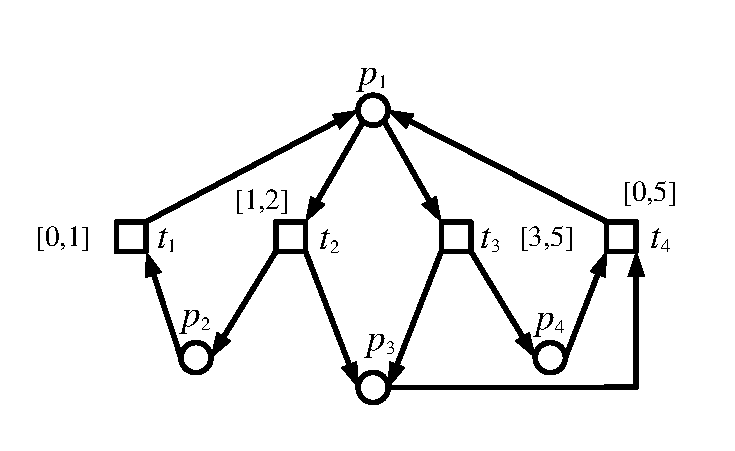
\includegraphics[scale=0.65,angle=0]{figures/figure3-1.pdf}\\
        \caption{一个TTPN模型}
    \end{figure}

    Petri网带有时间之后,原来的标识向量是无法表示此Petri网状态的所有信息。
    所以TTPN的标识除了包含库所中的托肯数,还包含了当前Petri网上每个变迁上的时钟信息。
    因此TTPN的标识需要包含两个元素,第一个元素描述库所状态,称作place-marking(简记作p-marking),
    第二个元素描述变迁状态,称为transition-marking(简记作t-marking)。
    p-marking即为普通Petri网的标识。
    t-marking表示了每个变迁上时钟的当前时间,如果此变迁不使能,则用符号$\nu$表示。

    \textbf{定义2.14}\cite{2013Time}\textbf{:}
    记$P$为时间网$Z$所有库所的集合,网$Z$的一个p-marking是一个从$P$到$\mathbb{N}$的映射:$P \rightarrow \mathbb{N}$。
    显然,时间网$Z$中的p-marking也是原网中的标识。

    \textbf{定义2.15}\cite{2013Time}\textbf{:}
    记$T$为时间网$Z$所有变迁的集合,时间网$Z$中的任意一个映射:$T \rightarrow \mathbb{R}_{0}^{+} \cup \{\nu\}$就是一个t-marking。

    \textbf{定义2.16}\cite{2013Time}\textbf{:}
    记$Z=(P,T,F,W,M_{0},I)$为一个时间Petri网,$m$为$Z$的一个p-marking,$h$为$Z$的一个t-marking,$Z$的一个状态为一个二元组$z=(m,h)$且:

    1. $\forall t ((t \in T \wedge t^{-} \nleq m) \rightarrow h(t) = \nu)$;

    2. $\forall t ((t \in T \wedge t^{-} \leq m) \rightarrow (h(t) \in \mathbb{R}_{0}^{+} \wedge h(t) \leq LFT(t)))$;

    状态$z_{0}=(m_{0},h_{0})$为时间网$Z$的初始状态,其中:

    $h_{0}(t)= \bigg \{\begin{array}{ll}
    0 & if \quad t^{-} \leq m_{0} \\
    \nu & if \quad t^{-} \nleq m_{0}
    \end{array}.$

    以上是时间网的静态特性。
    正如普通Petri网的动态特性是由发射规则所决定的,时间网的状态也与发射规则有关,时间网的当前状态会因为当前的p-marking或者t-marking的变化而改变。
    普通Petri网的p-marking会随着变迁的发射而改变,在时间网中,变迁的发射通常不仅改变当前的p-marking,也会改变t-marking。除了变迁的发射,t-marking也会随着时间的流逝而改变。

    \textbf{定义2.17}\cite{2013Time}\textbf{:}
    在时间网$Z=(P,T,F,W,M_{0},I)$中,变迁$t$在状态$z=(m,h)$下准备好发射的条件是:

    1. $t$在原网的标识$m$下是使能的,且$t^{-} \leq m$;

    2. $h(t) \geq EFT(t)$。

    \textbf{定义2.18}\cite{2013Time}\textbf{:}
    记$\hat{t}$和$z=(m,h)$分别为时间网$Z=(P,T,F,W,M_{0},I)$的一个变迁和一个状态,变迁$\hat{t}$能够在状态$z$下发射的条件是$\hat{t}$已经满足准备好发射的条件,
    记作$z \stackrel{\hat{t}}{\longrightarrow} $。$\hat{t}$发射之后,网$Z$的状态从$z$改变到$z^{'}=(m^{'},h^{'})$,记作$z \stackrel{\hat{t}}{\longrightarrow} z^{'}$,其中:

    1. $m^{'}=m+ \Delta \hat{t}$;

    2. $\forall t (t \in T \longrightarrow h^{'}(t)= \bigg \{\begin{array}{ll}
    \nu & if \quad t^{-} \nleq m^{'} \\
    h(t) & if \quad t^{-} \leq m \wedge t^{-} \leq m^{'} \wedge ^{\bullet}t \cap ^{\bullet}\hat{t} = \emptyset \wedge t \neq \hat{t} \quad )\\
    0 & otherwise
    \end{array}.$

    根据上述的定义,TTPN的每个变迁上都有一个时钟。
    此变迁使能以后,它上面的时钟开始计时,达到此变迁的最早发射时间后,此变迁允许被发射,但时钟上的时间不允许超过最迟发射时间。
    一旦变迁被发射、变得不使能或变迁前置库所中的托肯被改变,此变迁的时钟会重新计时。

    TTPN是由普通Petri网上添加时间区间得到的,但普通Petri网也可看做一种TTPN。即将普通Petri网所有的变迁的最早发射时间设为0,最迟发射时间设为无穷大,即时间区间为$[0,\infty]$。
    \subsection{时间库所网}
    时间库所网(Time Pace Petri Net,TPPN)即为在库所上添加时间限制的Petri网,每个进入库所的托肯,需要满足库所上的时间限制,才能被取走,这意味着每个托肯上都有一个时钟。

    \textbf{定义2.19}\cite{St2008Real}\cite{2012Reachability}\cite{Bonhomme2014Marking}\textbf{:}
    一个TPPN是一个六元组$Z=(P,T,F,W,M_{0},I)$,其中:

    1. 五元组$(P,T,F,W,M_{0})$是一个基本Petri网;

    2. $I:P \rightarrow (\mathbb{Q}_{0}^{+} \cup 0) \times (\mathbb{Q}_{0}^{+} \cup {\infty})$,$p_{i} \rightarrow I(p_{i})=[a_{i},b_{i}], 0 \leq a_{i} \leq b_{i} $。

    与TTPN的标识类似TPPN中也需要涵盖系统的时间信息。
    TPPN的时间区间加在库所上,但由于进入库所的托肯有先后顺序,因此同一个库所中的一系列托肯在时间上并不等价。
    要涵盖系统的完整信息,需要记录每一个托肯上的时钟。

    TPPN所有的托肯都是同步倒计时的,因此每进行一次发射,都要对所有的托肯重新计算其时钟。
    但是在本文第三章建立的实际晶圆制造系统的Petri网中,大部分库所是不存在时间约束的,为了提高之后算法效率,
    降低程序运行时间,本文的发射逻辑中会跳过无时间约束的库所中托肯的计时。

    \textbf{例2.9}\hspace{0.5em}
    如图2.7所示,是一个TPPN模型。其时间区间均添加在库所上,表示进入此库所的托肯如果要被取出,需要满足的时间限制。
    库所$p_{2}$中有两个托肯,假设这两个托肯是刚刚一起被放入这个库所中的,即这两个托肯上的时钟的计时为0。
    当变迁$t_{1}$发射后,会取走库所$p_{2}$中的一个托肯。
    这意味着$p_{2}$中至少有一个托肯的时钟计时超过了一个时间单位。
    TPPN中所有的托肯是同步计时的,当变迁$t_{1}$发射后,取走库所$p_{2}$中的一个托肯,
    如果要继续发射变迁$t_{1}$,是不需要消耗时间的,因为另一个托肯上的时钟也一并计时超过了一个时间单位

    \begin{figure}[H]
        \centering
        % Requires \usepackage{graphicx}
        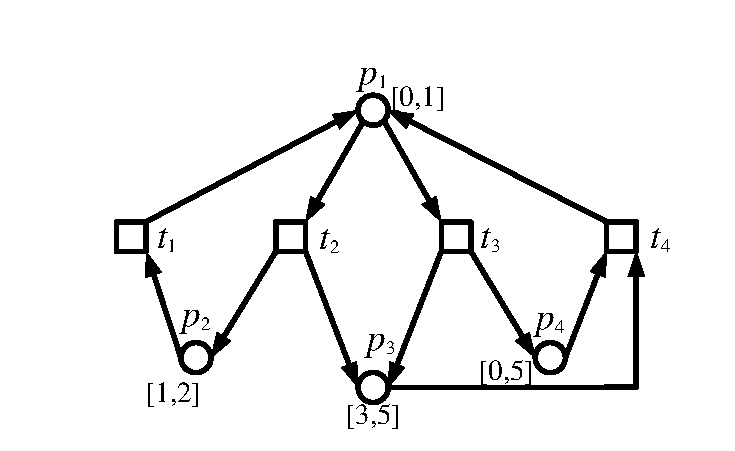
\includegraphics[scale=0.65,angle=0]{figures/figure3-2.pdf}\\
        \caption{一个TPPN模型}
    \end{figure}

    TTPN和TPPN的差异不仅仅是时间区间加在变迁或库所上这一点,他们时钟计时方式也有很大的区别。
    TTPN时钟加在变迁上,当变迁使能时,时钟开始计时,此变迁的前置库所中的托肯被更新过就会重置计时。
    而TPPN的时钟加在托肯上,会一直计时下去,托肯被移动才会重置时钟。

    基于以上的描述,TTPN和TPPN的计时方式并没有实质上的冲突,可以兼容起来。
    只需要将TTPN的变迁计时前判断库所使能的逻辑扩展为TPPN的使能逻辑就行了。
    本文为解决实际问题按此思路将TTPN和TPPN结合起来,提出了一种新的时间网子类。
\section{本章小结}
本章介绍了Petri网概念与特性、Petri网的应用、Petri网的调度方法和一系列时间网。
在接下来的章节中,将使用这些基础知识为实际系统进行建模,并使用调度算法对模型进行调度,并求解调度方案。
% \chapter{时间网与实际制造系统结合}

\section{变迁和库所上均有时延的时间Petri网}
假设存在一个场景,机械臂需要从加工腔中取走一个工件放入另一个加工腔,
工件在加工腔中加工需要时间,机械臂移动也需要时间。
如果将加工腔看作库所,工件看作托肯,机械臂的动作看作变迁,
则意味着托肯进入某库所后等待一段时间,
之后变迁开始计时一段时间后发射,
将此托肯移入另一个库所中。

因此需要一种新的时间Petri网模型,将TTPN和TPPN结合起来,本文提出了一种新的时间Petri网子类,时间变迁库所网(Time Transition Place Petri Net,TTPPN),
解决了这种场景下的建模问题。

TTPPN需要在变迁和库所上都添加时间区间。库所上的时间区间表示进入此库所的托肯,至少需要等待一段时间才能被取走,但不能驻留过长的时间。
普通Petri网的使能逻辑中某个库所是否使能只需要判断此库所中的托肯数是否大于其尝试发射后置变迁输入弧上的权值就行了,
也就是要保证库所中有足够的托肯能被取走。
但TTPPN库所的使能还需要看托肯上的时钟,
因为在TPPN中,托肯能否被取走,还需要判断托肯的停留时间是否满足了库所上的时间限制。
因此TTPPN库所能否使能,需要看此库所中满足此库所时间限制的托肯的个数是否不低于其尝试发射后置变迁输入弧上的权值。

\textbf{定义3.1}\textbf{:}
一个TTPPN是一个七元组$Z=(P,T,F,W,M_{0},I_{p},I_{t})$,其中:

1. 五元组$(P,T,F,W,M_{0})$是一个基本Petri网;

2. $I_{p}:P \rightarrow (\mathbb{Q}_{0}^{+} \cup 0) \times (\mathbb{Q}_{0}^{+} \cup {\infty})$,$p_{i} \rightarrow I(p_{i})=[a_{i},b_{i}], 0 \leq a_{i} \leq b_{i} $;

3. $I_{t}:P \rightarrow (\mathbb{Q}_{0}^{+} \cup 0) \times (\mathbb{Q}_{0}^{+} \cup {\infty})$,$t_{i} \rightarrow I(t_{i})=[a_{i},b_{i}], 0 \leq a_{i} \leq b_{i} $。

在TTPN中,变迁一旦使能,其上的时钟便会开始计时。在TTPPN中也是如此。
当此变迁的所有前置库所都使能的那一瞬间,此变迁的时钟开始计时。

在实际的制造系统中,完成工序的耗时是一个衡量控制策略的重要指标。
Petri网的变迁表示的是此系统能执行的动作。
为了让系统完成任务所执行的一系列的动作的耗时尽可能短,则要避免不必要的时间开销。
这意味着,变迁的发射应该尽可能早,变迁上的时钟不允许有无意义的计时。

为了实现这个需求,发射逻辑应该分为3部分:变迁发射前的逻辑、变迁发射的逻辑、变迁发射后的逻辑。
某变迁如果满足库所使能,并且需要被发射,须要按顺序执行完这3个逻辑。

\begin{algorithm}[H]
    \caption{变迁发射逻辑}
    \hspace*{0.02in} {\bf 输入:} 
    变迁库所时间网$TTPPN$,变迁库所时间网的标识$Marking$,准备发射的变迁$t$\\
    \hspace*{0.02in} {\bf 输出:}
	变迁$t$发射后到达的新标识$next$
    \begin{algorithmic}[1]
		\State $next \leftarrow $将$Marking$克隆一份
		\State $beforeTlanuch(TTPPN,next,t)$ //变迁发射前的逻辑
		\State $tlanuch(TTPPN,next,t)$ //变迁发射的逻辑
		\State $afterTlanuch(TTPPN,next,t)$ //变迁发射后的逻辑
		\State 返回$next$
    \end{algorithmic}
\end{algorithm}

变迁发射前的逻辑要实现两个目标:1、计算出使此变迁使能的最短时间。2、从对应库所中删除被此变迁取走的托肯。
变迁如果要使能,则其前置库所中需要有足够多完成计时的托肯。
因此变迁使能的最短时间为此变迁所有前置库所中,所有被取走托肯中计时离时间限制最长的那段时间。
如果将时钟改为倒计时,此时间应该为被取走的托肯中倒计时最长的那个时间。
为了避免消耗不必要的时间,对于特定库所,取走的托肯应该是最先完成倒计时的那一批。


\begin{algorithm}[H]
	\caption{变迁发射前的逻辑}
	\label{alg3-2}
	\begin{algorithmic}
		\Procedure{beforeTlanuch}{$TTPPN$,$next$,$t$}
		\ForAll{$p \in {\bullet}t$}
		\State $needGetCount \leftarrow Pre(p,t)$
		\State $minTime \leftarrow$ 标识$next$库所$p$中第$needGetCount$的时钟计时 
		\State $time \leftarrow max(time,minTime) $// $time$为使变迁$t$使能的最短时间
		\ForAll{$token \in TOKEN(p)$} //$TOKEN(p)$ 为库所$p$中的托肯的集合
		\If{$TIME(token) \le minTime$} //$TIME(token)$ 为此token上时钟的计时
		\State 从$TOKEN(p)$中删除$token$
		\EndIf
		\EndFor
		\EndFor
		\EndProcedure
	\end{algorithmic}
\end{algorithm}

按上述流程变迁$t$取托肯时总是从托肯序列的头部取,之后的流程会在托肯序列的尾部放入托肯。
而托肯在库所中停留会导致托肯时钟倒计时。
因此托肯序列必然是升序的。

此处托肯序列选取何种数据结构实现会影响到算法效率。
基于上述分析对托肯序列会有两种操作:
从序列头部删除托肯、从序列尾部添加托肯。
上述需求有两种实现方式:
链表、循环数组。

如果使用链表,即需要定义节点结构。
节点由两部分组成:托肯倒计时时钟、下一个节点的地址。
这将带来以下两个缺陷。

\begin{figure}[H]
	\centering
	% Requires \usepackage{graphicx}
	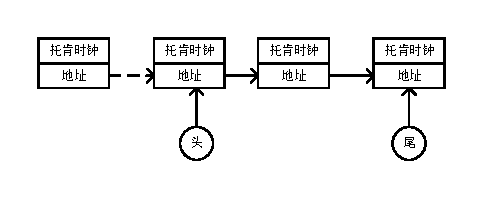
\includegraphics[scale=1.00,angle=0]{figures/托肯序列_链表.pdf}\\
	\caption{托肯序列的链表实现}
\end{figure}

为了将托肯连接成串,额外存储了大量地址信息。
如果地址和托肯时钟选取相同的数据类型,那么整个数据结构只有一半的有效信息。

当托肯被移除后,此节点便失去引用成为内存垃圾。
清理内存垃圾会带来时间开销。
添加新的托肯需申请新的托肯节点,申请内存亦会带来时间开销。
因此从时间和空间来看,链表这种数据结构实现托肯序列的功能并不高效。

本算法使用循环数组来实现此功能。
预先申请固定长度的数组,并保存头尾两个指针。
当删除托肯时头指针向前移动,如果已经移动到数组尾部,则从头开始。
当添加托肯时,尾指针向前移动,如果已经移动到数组尾部,则从头开始。
当尾指针追上头指针时,意味着数组已满。
需重新申请更大的数组,并将数据移入完成扩容。

\begin{figure}[H]
	\centering
	% Requires \usepackage{graphicx}
	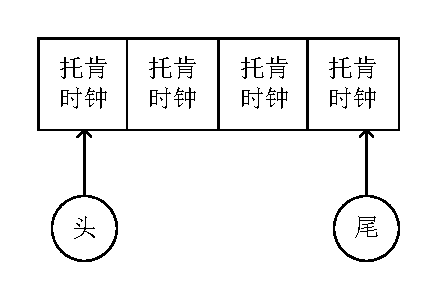
\includegraphics[scale=1.00,angle=0]{figures/托肯序列_循环数组.pdf}\\
	\caption{托肯序列的循环数组实现}
\end{figure}

循环数组中保留的信息只有托肯时钟,并且添加、删除托肯时如不发生扩容,均不会申请新内存。
如果发生扩容,也是一次申请连续内存,效率高于链表的每次申请单个节点。

变迁发射的逻辑要实现两个目标:1、计算出此变迁发射的总耗时。2、更新其他使能变迁的时钟。
变迁发射的总耗时即为之前求出的变迁使能的最短时间加上此变迁上的时钟。
但是其他变迁有可能在此变迁发射的整个过程中(包过为了让此变迁使能,之前托肯的倒计时过程)使能计时了,
因此需要在此环节一并更新他们的时钟。
这意味着需要对此时库所使能的变迁计算其使能的最短时间,其计算逻辑与变迁发射前的逻辑中的类似。

变迁发射的逻辑是三段逻辑中最为繁琐的,库所时间网和变迁时间网的特点都会在这段逻辑上体现出来。
在变迁时间网中,变迁发射后所有使能变迁是同步开始继续计时的,但结合上库所时间网变迁计时存在先后差异。
因此需要计算出其他变迁提前计时的情况,并更新变迁上时钟。

\begin{algorithm}[H]
	\caption{变迁发射时的逻辑}
	\label{alg3-3}
	\begin{algorithmic}
		\Procedure{tlanuch}{$TTPPN$,$next$,$t$}
		\State $timer \leftarrow TIME(t)$ //$TIME(t)$ 为标识$next$变迁$t$上时钟的倒计时的时间数值
		\State $time=time+timer$
		\ForAll{$t_{other} \in T$}
		\If{$t_{other}^{-} \le m$}
		\State $needGetCount \leftarrow Pre(p,t)$
		\State $minTime \leftarrow 库所p中第needGetCount大的时钟计时 $
		\If{$minTime \le time$}
		\State $TIME(t_{other})=TIME(t_{other})-time+minTime$
		\If{$TIME(t_{other}) \le 0$}
		$TIME(t_{other}) = 0$
		\EndIf
		\EndIf
		\EndIf
		\EndFor
		\EndProcedure
	\end{algorithmic}
\end{algorithm}

变迁发射后的逻辑要实现三个目标:1、对此Petri网所有托肯进行计时.2、对需要重置时钟的变迁,重置其时钟。3、对此变迁的后置库所放入托肯。
TTPPN托肯上的时钟是始终在计时的,因此需要对目前Petri网中的托肯上的倒计时时钟减去变迁发射的总耗时。
当某变迁的前置库所被别的变迁取走过托肯,此变迁上的时钟需要被重置。
当前发射的变迁上的时钟也需要被重置。
变迁发射后,其后置库所会被放入托肯,这些新放入的托肯上的倒计时时钟为库所时延。

在实际的制造系统中,并非所有库所上都有时间约束,因此并不需要对Petri网中的所有托肯重新计算时钟。
当某库所上没有时间约束时,应该跳过计时逻辑。
这段优化在实际情况下有显著效果,因为在建模时会加入额外的控制库所,这类库所中的托肯数往往会远高于其他库所,如果不跳过这些托肯的时钟计算,会浪费大量算力。
\begin{algorithm}[H]
	\caption{变迁发射后的逻辑}
	\label{alg3-4}
	\begin{algorithmic}
		\Procedure{afterTlanuch}{$TTPPN$,$next$,$t$}
		\ForAll{$p \in P$}
		\If{标识$next$库所$p$上没有时间约束}
		\State 跳过计时
		\EndIf
		\ForAll{$token \in TOKEN(p)$}
		\State $TIME(token)=TIME(token)-time$
		\If{$TIME(token)<0$}
		\State $TIME(token)=0$
		\EndIf
		\EndFor
		\EndFor
		\ForAll{$p \in$ $^{\bullet}t$}
		\ForAll{$t_{other} \in p^{\bullet}$}
		\State $TIME(t_{other})=0$
		\EndFor
		\EndFor
		\ForAll{$p \in t^{\bullet}$}
		\State $needPutCount \leftarrow Post(p,t)$
		\For{$i \leftarrow 1, needPutCount$}
		\State 将$token$添加进$TOKEN(p)$中
		\State $[a,b] \leftarrow I_{p}(p)$
		\State $TIME(token)=a$
		\EndFor
		\EndFor
		\EndProcedure
	\end{algorithmic}
\end{algorithm}

上述逻辑发射解决了时间区间有下界无上界的情况。
例如某托肯在库所中最早需要停留3个时间单位,当不能超过5个时间单位,
使用上述逻辑还不能实现。
本文对于这种情况的实现思路为:
直接将超过上界约束的标识设置为死锁标识,令其所有的变迁均无法使能。

之后调度算法在发射变迁$t$时会先判断此变迁能否使能。
如果能使能,则发射此变迁。

\begin{algorithm}[H]
    \caption{使能判断逻辑}
    \label{}
    \hspace*{0.02in} {\bf 输入:} 
    变迁库所时间网$TTPPN$,变迁库所时间网的标识$Marking$,准备发射的变迁$t$\\
    \hspace*{0.02in} {\bf 输出:}
	布尔值
    \begin{algorithmic}[1]
		\If{此标识$Markintg$超过时间约束}
		\State return false
		\EndIf
		\State return 发射变迁$t$标识$Marking$是否满足库所使能要求
    \end{algorithmic}
\end{algorithm}

如下图所示,这是一个库所变迁时延网的模型。
一共有四个变迁和四个库所。库所$p_{2}$中有两个托肯,其余的库所中均没有托肯。
所有的库所和变迁上均有时间约束。
库所上的时间约束既有上界又有下届。
而变迁上的时间约束只有上界。

\begin{figure}[H]
	\centering
	% Requires \usepackage{graphicx}
	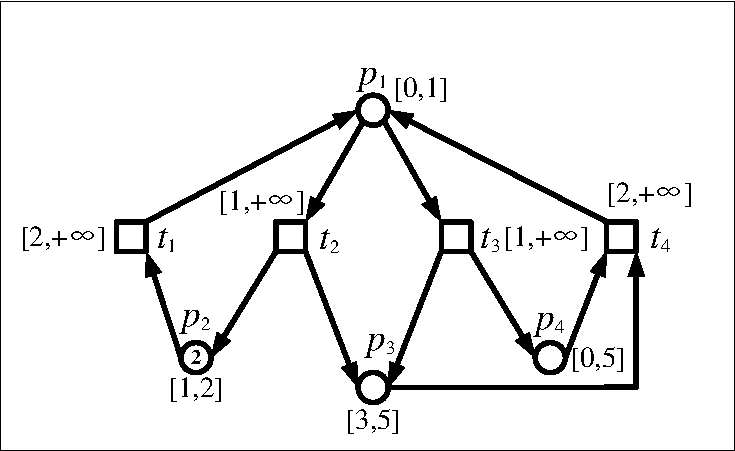
\includegraphics[scale=1.00,angle=0]{figures/TTPPN.pdf}\\
	\caption{一个库所变迁时间网的例子}
\end{figure}

初始情况下库所$p_{4}$中没有托肯,当$p_{4}$中被移入1个托肯作为目标。
有以下的调度策略:$t_{1}->t_{3}$。
其中标识的序列为:$M_{1}:(0,2,0,0)$ 全局时间:0,变迁使能时间:0;
$M_{2}:(1,1,0,0)$ 全局时间:3,变迁使能时间:1;
$M_{3}:(0,1,1,1)$ 全局时间:4,变迁使能时间:3。

标识$M_{2}$是变迁$t_{1}$发射后生成的。
$t_{1}$需要从$p_{2}$中取走一个托肯,
如果要使能,必须等待其唯一的前置库所$p_{2}$中的一个托肯完成倒计时。
因此$t_{1}$的最小使能时间是1个时间单位。
同时Petri网中的其他托肯会同时倒计时,这意味着$p_{2}$中所有的托肯都完成了倒计时。
$t_{1}$发射后,如果$p_{2}$还需要被取走一个托肯,那么取走它的变迁是可以直接使能的。

$t_{1}$使能后,至少需要等待2个时间单位才能发射。
因此$M_{2}$的全局时间为3个时间单位。

$t_{3}$需要从$p_{1}$中取走一个托肯。
而$p_{1}$中的托肯不需要等待就可以被取走,因此$t_{3}$可以立刻使能。
本程序会尽可能的减少无意义的驻留,所以$t_{3}$的使能时间即为$M_{2}$生成的最早的全局时间,
也就是3个时间单位即可使能。
使能后至少需要1个时间单位才可以发射,
因此$M_{3}$的全局时间为4个时间单位。

\section{Petri网调度算法项目的架构设计}
本文为我研究生期间参与某半导体企业设计晶圆制造的预研项目的研究。
此项目的目标为对实际的晶圆制造系统进行调度。
因此需要按要求对系统进行建模,并使用调度算法对模型求解调度策略。

我负责算法的设计与开发。
对此类系统进行建模的方式有许多种,在项目初期,本项目组负责建模的同学尝试了变迁时间网、库所时间网等多种时间网进行建模。
同样的,求解Petri网调度策略的算法也有很多种,有经典的图搜索算法也有群体智能算法。
因此我设计了一个求解各种Petri网模型的调度算法集合的程序架构。

此架构使用Java语言开发,整体分为3个接口:Marking、PetriNet、Search。

Marking表示系统状态,比如库所向量,变迁、库所上的时钟会在这个接口的实现类中声明。
因为调度算法中频繁使用哈希表,所以根据系统状态求取哈希值的方法也在此接口实现类中声明。

PetriNet存有系统的结构,是用于实现系统状态转移的。
结合Petri网的实际背景,此接口主要对外提供两个方法,发射和判断使能。
调度算法一般会遍历所有变迁,使用此接口判断变迁是否使能,
如果能够使能再根据实际情况,选择是否发射此变迁。
使用发射方法时,会传入一个变迁,此接口的实现类内部会有当前系统的状态,发射方法完成时会返回发射变迁后系统的下一个状态,也就是返回一个Marking接口的对象。
调度算法得到此对象后,可以更新系统的当前状态,并进行接下来的循迹。

Search接口对外提供一个search方法,使用此方法后会返回一个解对象,包含标识序列和变迁序列。
变迁序列即为算法得到的调度策略,
标识序列为系统按调度策略运行时各个阶段的状态。

本架构的优点为使用接口改变了算法和模型的依赖关系,实现了解耦。
通常情况下,模型的底层环节,算法是顶层环节,算法依赖于模型。
使用本架构后,算法依赖于模型的接口,具体模型去实现模型接口,更换模型时不需要修改算法。

之后本人一直使用此程序架构进行开发,在模型层面先后编写了普通Petri网、变迁时间网、库所时间网、变迁库所时间网等代码;
在算法层面开发了A星算法、蚁群算法、遗传算法、贪心算法等算法。

\begin{figure}[H]
	\centering
	% Requires \usepackage{graphicx}
	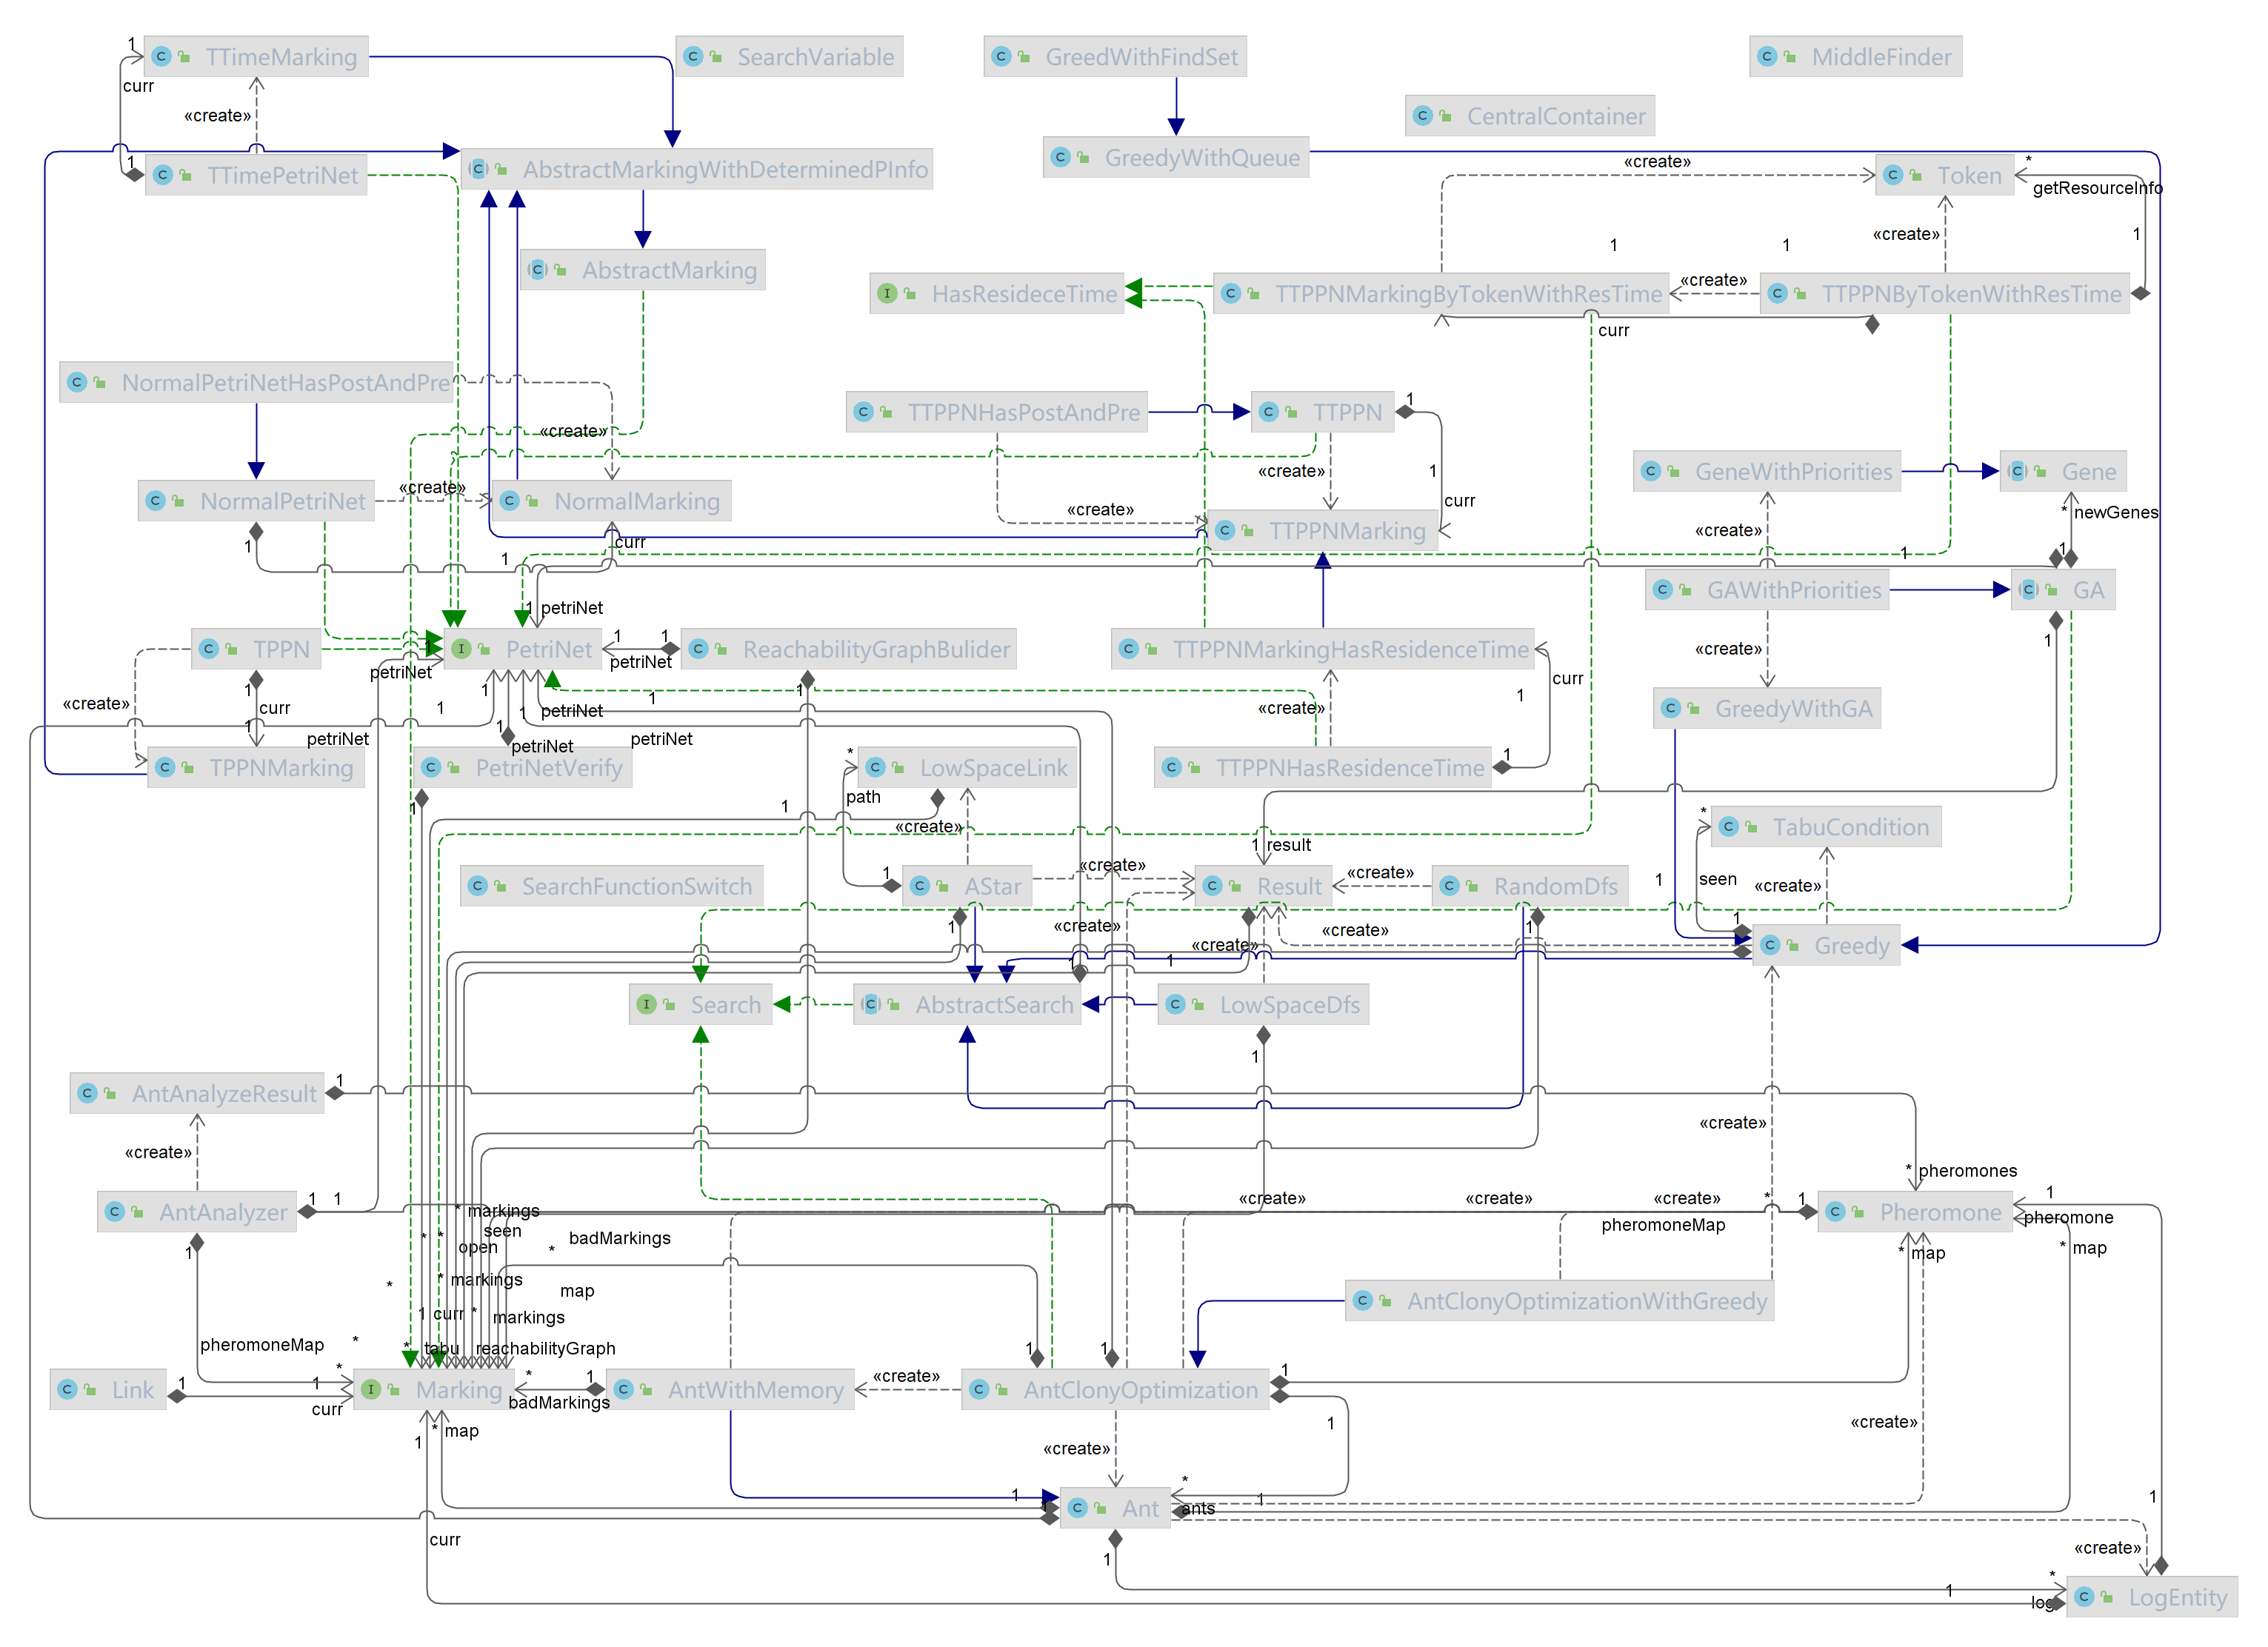
\includegraphics[width=\linewidth]{figures/架构图.png}\\
	\caption{算法程序架构图}
\end{figure}

目前程序架构如图所示。

\section{使用库所变迁时间网对实际制造系统进行建模}
前文介绍了各种时间网,并结合变迁时间网和库所时间网提出一种新的时间网子类:变迁库所时间网(TTPPN),
以及设计了一套TTPPN变迁发射流程,保证了发射变迁后系统全局时间尽可能早,
供之后的调度算法使用。

本节将使用上一节提出的TTPPN对一个实际的晶圆制造系统进行建模。
模型来源于2022年第六届全国大学生集成电路创新创业大赛(北方华创杯)。

\subsection{使用Petri网对晶圆制造系统建模的特点}
晶圆的加工制造包含多种工艺,需要多种设备协同完成,这些设备的组合运行导致了集束生产设备的高度复杂性。
另外,相比传统的仅能完成单一工艺流程的固定生产线,晶圆制造需要灵活的工艺方案以及多种工艺流程同时进行。
因此组合设备的调度方案需要不断更换,这导致设备调试以及调度方案成本过高。
本文将使用 Petri 网工具建立数学模型反应晶圆加工中双臂组合设备运行情况,
基于此研究满足约束的调度方案,并将 Petri 网相关的建模、调度理论应用于晶圆加工制造设备的运行控制。

Petri 网是一种适合于柔性制造系统的形式化方法:对非形式化需求做形式化处理时有助于发现歧义、矛盾;
系统的形式化模型可以帮助得到半自动甚至全自动的系统开发方法;
可以用数学方法验证形式化模型的正确性而避免对每种情况逐一测试;
经过形式验证的子系统可以并入更大系统;形式化模型允许不同设计方法相比较。

一个 Petri 网包含两种节点,称为库所和变迁,分别由圆圈和矩形表示。库所和变迁通过有向弧连接,
指定出 Petri 网运行的动态规律。用 Petri 网建模制造系统时,通常用库所表示资源和工序的状态,
用变迁表示工序事件的发生或起止,库所中的小黑点称为托肯,记录对应资源的数量。

时间是生产调度的根本参考,因此本文将使用时延 Petri 网对晶圆制造设备建模,包括 T-时间 Petri 网(TPN),
每个变迁将被指定一个时间区间,该变迁仅在给定时间区间内才可以发生,和变迁库所时延网(TTPPN),
变迁仅在给定时间区间内才可以发生且库所中的托肯在给定时间区间才被视作可使用的。
一旦变迁到达时间区间的上限,该变迁将强制发射(强语义)。
若一个变迁被多重允许,即当前资源可以保证一项工序执行两次及以上,每次变迁发射后时间约束将重新计算(单服务器)。

\subsection{基于工序的建模方法进行建模}
晶圆的加工流程可以视为由四个典型工序组成:校准、进料、加工工序、以及冷却并出料。
此处以图4.1所示设备为例,加工配方为从 LP1 中取得晶圆放入校准模块 AL,
校准完成后放入真空锁 LL 的 S2 槽位,在 PM3 或 PM4 中执行第一道工序,在 PM1、 2、 5、6 中执行第二道工序,
放入 LL 中的 S1 槽位冷却完成后取出放回 LP1。

该配方要求每个晶圆按顺序进行 5 个工序,因此使用序号 0-5 依次表示晶圆状态。
其中校准、进料工序由机械手 TM1 调度,工序 1、工序 2 由机械手 TM2 调度,冷却并出料由 TM1、 TM2 协作完成。
加工过程中,机械手 TM1、 TM2 的移动,真空锁的转换,
加工模块的加工是相对独立的子模块,机械手对晶圆的取放调度是主要的加工流程,
因此按照工序划分后描述并给出相应的关联矩阵。

\begin{figure}[H]
	\centering
	% Requires \usepackage{graphicx}
	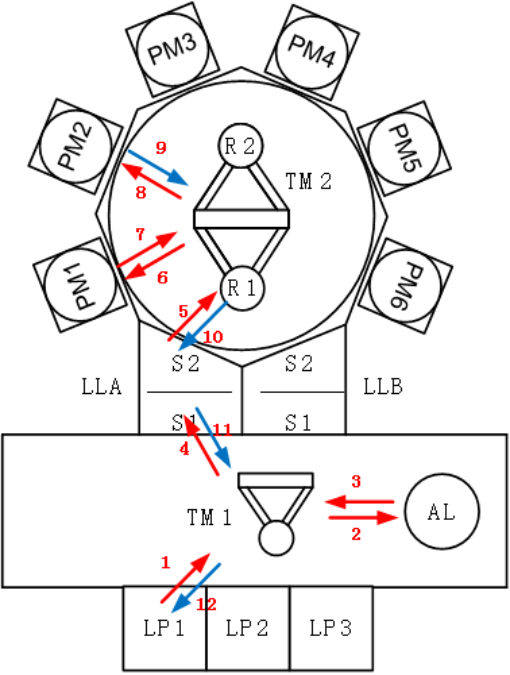
\includegraphics[scale=0.8,angle=0]{figures/4-1.png}\\
	\caption{晶圆制造系统}
\end{figure}

\subsubsection{库所与变迁的命名}
首先对文中将要出现的库所和变迁的命名规则加以说明:
\begin{enumerate}
	\item 库所表示系统中的各种资源,可以分为机械手 TM1 和 TM2 的位置,处于不同位置不同状态的晶圆,各加工模块的物理容量,真空锁状态四类:
	      \begin{enumerate}
		      \item 机械手 TM1 和 TM2 的位置: TM1 的可能位置集合 A ={LP1, AL, LLA, LLB},
		            将对应库所的标签命名为 TM1ata,其中 a $\in$ A,意为机械手 TM1 处于 a 位置;
		            TM2 中 R1 机械手所处位置集合 B ={PM1, PM2, PM3, PM4, PM5, PM6,
		            LLA, LLB}, R1atb,其中 b $\in$ B,意为机械手 R1 处于 b 位置,同时 R2 与
		            R1 处在相对位置。
		      \item 处于不同位置不同状态的晶圆:其中晶圆可能被放置的位置集合 C ={LP1,
		            AL, PM1, PM2, PM3, PM4, PM5, PM6, AS1, AS2, BS1, BS2},机械手集
		            合 D ={TM1, R1, R2},晶圆状态包括 E ={0, 1, 2, 3, 4, 5},因此我们用库所
		            eatc、 eind 分别表示 e 状态晶圆处于 c 位置以及处于 d 机械手,库所中托肯的
		            数量代表了相应资源的个数。注意,并非所有组合都有对应库所,例如 0atAS1,
		            因为加工过程中不会把未校准的晶圆放入真空锁,具体使用到的库所和变迁会
		            在后文分工序描述。
		      \item 各加工模块的物理容量:晶圆可能被放置在位置集合 C ={LP1, AL, PM1, PM2,
		            PM3, PM4, PM5, PM6, AS1, AS2, BS1, BS2} 或机械手集合 D ={TM1, R1,
		            R2},这些位置的物理容量用库所 ccap 或者 dcap 来表示,库所中的托肯数代
		            表了这些位置的容量。以及一个特殊的库所 motor 代表机械手 TM2 取放操作
		            的电机是否空闲。
		      \item 真空锁状态:真空锁集合 F ={LLA, LLB},真空锁的状态集合 G ={v, nv},
		            用 fg 表示真空锁 f 处于状态 g, 其中 v 表示真空状态, nv 表示大气状态。
	      \end{enumerate}
	\item 变迁同样分为四类,主要包括机械手取放各模块上的晶圆、机械手的移动、真空锁状态的切换、各加工模块的加工:
	      \begin{enumerate}
		      \item 机械手取放各模块上的晶圆: 机械手集合 D ={TM1, R1, R2},晶圆可能被放
		            置的位置集合 C ={LP1, AL, PM1, PM2, PM3, PM4, PM5, PM6, AS1, AS2,
		            BS1, BS2},用 dpickc, ddropc 分别表示机械手 d 将晶圆从位置 c 拿起或放入
		            位置 c。
		      \item 机械手的移动: TM1 的可能位置集合 A ={LP1, AL, LLA, LLB}, TM2 中 R1
		            机械手位置集合 B ={PM1, PM2, PM3, PM4, PM5, PM6, LLA, LLB},用
		            a − a′, b − b′ 分别表示 TM1 从位置 a 移动到 a′, R1 从位置 b 移动到 b′,其
		            中 a, a′ $\in$ A, b, b′ $\in$ B。
		      \item 真空锁状态的切换:真空锁集合 F ={LLA, LLB},真空锁的状态集合 G ={v,
		            nv},用 Ag − g′, Bg − g′ 分别表示真空锁 A, B 由状态 g 切换到 g′,其中
		            g, g′ $\in$ G。
		      \item 各加工模块的加工: 加工模块集合 H ={AL, PM1, PM2, PM3, PM4, PM5,
		            PM6},用 hwork 表示加工模块 h 执行加工程序。另外,用 LLAcd, LLBcd 分
		            别表示晶圆在 LLA, LLB 执行冷却工序。
	      \end{enumerate}
\end{enumerate}
\subsection{主要功能模块}
在晶圆加工需要的工序之外,存在部分子模块独立于主系统运行,他们的运行主要取
决于自身的运行规律,同时对主系统中的操作其限制作用。在 Petri 网中表现为独立子网,
其中所有变迁的前置库所都包含在子网内部。案例中的机械手移动,真空锁的状态切换,
加工模块 PM 对晶圆的加工操作都是独立于主系统运行的功能模块。例如机械手移动,仅
与当前位置相关,而机械手的位置是主系统一些操作的必要条件。因此可以对各功能模块
建立的子 Petri 网可以直接用来并入总 Petri 网。
\subsubsection{机械手移动模块}
样例模型包含机械臂 TM1 和机械臂 TM2,其中 TM2 包含两个机械手 R1 和 R2,相
对布置。 TM1 的可能位置集合 A ={LP1, AL, LLA, LLB},共 4 个,将对应库所的标签
命名为 TM1ata,其中 a $\in$ A,意为机械手 TM1 处于 a 位置。同样的, TM2 的位置用
R1 所处位置来表示,共 8 个,位置集合 B ={PM1, PM2, PM3, PM4, PM5, PM6, LLA,
LLB},将对应库所的标签命名为 R1atb,其中 b $\in$ B,意为机械手 R1 处于 b 位置。系统
初始状态时, R1 处于 LLA 处, TM1 处于 LP1 处。

根据加工顺序要求,单个晶圆的移动包括从仓储 LP1 中取出放入校准模块 AL,从
AL 放入真空锁 LLA 或 LLB,最后从 LLA 或 LLB 取出放回 LP1。考虑到多个晶圆同时
加工的情况,提到的 3 个步骤会乱序发生,因此需要加入必要的移动变迁保证 TM1 的连
续移动。移动变迁的发射仅仅与机械手位置有关,以 LP1-AL 为例,它的发生需要 TM1
处于当前位置 LP1,发生后使得 TM1 位置处于 AL。

TM2 的移动包括机械手 R1、 R2 分别将晶圆从真空锁 LLA 或 LLB 取出放到第一道
工序的加工模块 PM3 或 PM4,再从 PM3 或 PM4 取出放入第二道工序的加工模块 PM1、PM2、 PM5 或 PM6,最后从第二道工序模块取出放入真空锁 LLA 或 LLB,以及各变迁
乱序发生时必要的移动。为了简洁,此处仅列出单个晶圆由 R1 执行各工序需要的移动变
迁,实际建模可以考虑列出所有 7 $\times $ 6 个变迁。

\begin{center}
	\textbf{TM1 与 TM2 位置库所}\\
	\resizebox{!}{!}{
		\begin{tabular}{llll}
			\toprule
			编号 & 库所     & 释义                                   & 初始托肯数 \\
			\hline
			$p_{1}$   & R1atPM1  & 机械手 R1 处于 PM1, 机械手 R2 处于 PM5 & 0          \\
			$p_{2}$   & R1atPM2  & 机械手 R1 处于 PM2, 机械手 R2 处于 PM6 & 0          \\
			$p_{3}$   & R1atPM3  & 机械手 R1 处于 PM3, 机械手 R2 处于 LLB & 0          \\
			$p_{4}$   & R1atPM4  & 机械手 R1 处于 PM4, 机械手 R2 处于 LLA & 0          \\
			$p_{5}$   & R1atPM5  & 机械手 R1 处于 PM5, 机械手 R2 处于 PM1 & 0          \\
			$p_{6}$   & R1atPM6  & 机械手 R1 处于 PM6, 机械手 R2 处于 PM2 & 0          \\
			$p_{7}$   & R1atLLA  & 机械手 R1 处于 LLA, 机械手 R2 处于 PM3 & 1          \\
			$p_{8}$   & R1atLLB  & 机械手 R1 处于 LLB, 机械手 R2 处于 PM4 & 0          \\
			$p_{9}$   & TM1atLP1 & 机械手 TM1 处于 LP1                    & 1          \\
			$p_{10}$  & TM1atAL  & 机械手 TM1 处于 AL                     & 0          \\
			$p_{11}$  & TM1atLLA & 机械手 TM1 处于 LLA                    & 0          \\
			$p_{12}$  & TM1atLLB & 机械手 TM1 处于 LLB                    & 0          \\
			\bottomrule
		\end{tabular}
	}
\end{center}

\begin{center}
	\textbf{TM1 移动变迁}\\
	\resizebox{!}{!}{
		\begin{tabular}{lllll}
			\toprule
			编号 & 变迁    & 释义                  & 前置库所 & 后置库所 \\
			\hline
			$t_{1}$   & LP1-AL  & 从 LP1 运动到 AL      & TM1atLP1 & TM1atAL  \\
			$t_{2}$   & AL-LLA  & 从 AL 运动到 LLA      & TM1atAL  & TM1atLLA \\
			$t_{3}$   & AL-LLB  & 从 AL 运动到 LLB      & TM1atAL  & TM1atLLB \\
			$t_{4}$   & LLA-LLB & 从 LLA 运动到 LLB     & TM1atLLA & TM1atLLB \\
			$t_{5}$   & LLB-LLA & 从 LLB 运动到 LLA     & TM1atLLB & TM1atLLA \\
			$t_{6}$   & LLA-LP1 & 从 LLA 运动到 LP1     & TM1atLLA & TM1atLP1 \\
			$t_{7}$   & LLB-LP1 & TM1 从 LLB 运动到 LP1 & TM1atLLB & TM1atLP1 \\
			\bottomrule
		\end{tabular}
	}
\end{center}

\begin{center}
	\textbf{TM2 移动变迁}\\
	\resizebox{!}{!}{
		\begin{tabular}{lllll}
			\toprule
			编号 & 变迁    & 释义                    & 前置库所 & 后置库所 \\
			\hline
			$t_{8}$   & LLA-PM3 & R1 从 LLA 运动到 PM3    & R1atLLA  & R1atPM3  \\
			$t_{9}$   & LLA-PM4 & R1 从 LLA 运动到 PM4    & R1atLLA  & R1atPM4  \\
			$t_{10}$  & LLB-PM3 & 从 R1 从 LLB 运动到 PM3 & R1atLLB  & R1atPM3  \\
			$t_{11}$  & LLB-PM4 & R1 从 LLB 运动到 PM4    & R1atLLB  & R1atPM4  \\
			$t_{12}$  & PM3-PM1 & R1 从 PM3 运动到 PM1    & R1atPM3  & R1atPM1  \\
			$t_{13}$  & PM3-PM2 & R1 从 PM3 运动到 PM2    & R1atPM3  & R1atPM2  \\
			$t_{14}$  & PM3-PM5 & R1 从 PM3 运动到 PM5    & R1atPM3  & R1atPM5  \\
			$t_{15}$  & PM3-PM6 & R1 从 PM3 运动到 PM6    & R1atPM3  & R1atPM6  \\
			$t_{16}$  & PM4-PM1 & R1 从 PM4 运动到 PM1    & R1atPM4  & R1atPM1  \\
			$t_{17}$  & PM4-PM2 & R1 从 PM4 运动到 PM2    & R1atPM4  & R1atPM2  \\
			$t_{18}$  & PM4-PM5 & R1 从 PM4 运动到 PM5    & R1atPM4  & R1atPM5  \\
			$t_{19}$  & PM4-PM6 & R1 从 PM4 运动到 PM6    & R1atPM4  & R1atPM6  \\
			$t_{20}$  & PM1-LLA & R1 从 PM1 运动到 LLA    & R1atPM1  & R1atLLA  \\
			$t_{21}$  & PM1-LLB & R1 从 PM1 运动到 LLB    & R1atPM1  & R1atLLB  \\
			$t_{22}$  & PM2-LLA & R1 从 PM2 运动到 LLA    & R1atPM2  & R1atLLA  \\
			$t_{23}$  & PM2-LLB & R1 从 PM2 运动到 LLB    & R1atPM2  & R1atLLB  \\
			$t_{24}$  & PM5-LLA & R1 从 PM5 运动到 LLA    & R1atPM5  & R1atLLA  \\
			$t_{25}$  & PM5-LLB & R1 从 PM5 运动到 LLB    & R1atPM5  & R1atLLB  \\
			$t_{26}$  & PM6-LLA & R1 从 PM6 运动到 LLA    & R1atPM6  & R1atLLA  \\
			$t_{27}$  & PM6-LLB & R1 从 PM7 运动到 LLB    & R1atPM6  & R1atLLB  \\
			\bottomrule
		\end{tabular}
	}
\end{center}

\subsubsection{真空锁模块}
真空锁抽气与充气的动作是独立进行的。此处共有两个真空锁 LLA 和 LLB, LLA 与
LLB 的抽气与充气动作互相独立,动作一旦开始就不会中止:

\begin{center}
	\textbf{TM2 移动变迁}\\
	\resizebox{!}{!}{
		\begin{tabular}{llll}
			\toprule
			编号 & 库所 & 释义             & 初始托肯数 \\
			\hline
			$p_{13}$  & Av   & LLA 处于真空状态 & 0          \\
			$p_{14}$  & Anv  & LLA 处于大气状态 & 1          \\
			$p_{15}$  & Bv   & LLB 处于真空状态 & 0          \\
			$p_{16}$  & Bnv  & LLB 处于大气状态 & 1          \\
			\bottomrule
		\end{tabular}
	}
\end{center}

\begin{center}
	\textbf{真空锁变迁}\\
	\resizebox{!}{!}{
		\begin{tabular}{lll}
			\toprule
			编号 & 变迁  & 释义                 \\
			\hline
			$t_{28}$  & Av-nv & LLA 由真空转为大气态 \\
			$t_{29}$  & Anv-v & LLA 由大气转为真空态 \\
			$t_{30}$  & Bv-nv & LLB 由真空转为大气态 \\
			$t_{31}$  & Bv-v  & LLB 由大气转为真空态 \\
			\bottomrule
		\end{tabular}
	}
\end{center}

\begin{center}
	\textbf{真空锁关联矩阵}\\
	\resizebox{!}{!}{
		\begin{tabular}{l|llll}
			\toprule
			Pre/Post & Av-nv & Anv-v & Bv-nv & Bnv-v \\
			\hline
			Av       & 1/0   & 0/1   &       &       \\
			Anv      & 0/1   & 1/0                   \\
			Bv       &       & 1/0   & 0/1           \\
			Bnv      &       & 0/1   & 1/0           \\
			\bottomrule
		\end{tabular}
	}
\end{center}


\subsubsection{独立加工模块}
加工模块与系统的其他工作互不冲突,一旦原料进入,加工模块开始加工直到工序完
成,罗列如下:
\subsection{主要加工工序}
\subsubsection{校准工序}
校准工序包含机械手 TM1 取出 LP1 中未加工晶圆,放入校准模块 AL,校准完成后
取出校准后晶圆,这里认为校准过程需要 TM1 参与。
根据加工要求,前置关联矩阵与后置关联矩阵如下:

\begin{center}
	\textbf{校准工序库所}\\
	\resizebox{!}{!}{
		\begin{tabular}{llll}
			\toprule
			编号 & 库所   & 释义                     & 初始托肯数 \\
			\hline
			$p_{17}$  & 2atPM3 & 待加工晶圆在加工模块 PM3 & 0          \\
			$p_{18}$  & 2atPM4 & 待加工晶圆在加工模块 PM4 & 0          \\
			$p_{19}$  & 3atPM3 & 已加工晶圆在加工模块 PM3 & 0          \\
			$p_{20}$  & 3atPM4 & 已加工晶圆在加工模块 PM4 & 0          \\
			$p_{21}$  & 3atPM1 & 待加工晶圆在加工模块 PM1 & 0          \\
			$p_{22}$  & 3atPM2 & 待加工晶圆在加工模块 PM2 & 0          \\
			$p_{23}$  & 3atPM5 & 待加工晶圆在加工模块 PM5 & 0          \\
			$p_{24}$  & 3atPM6 & 待加工晶圆在加工模块 PM6 & 0          \\
			$p_{25}$  & 4atPM1 & 已加工晶圆在加工模块 PM1 & 0          \\
			$p_{26}$  & 4atPM2 & 已加工晶圆在加工模块 PM2 & 0          \\
			$p_{27}$  & 4atPM5 & 已加工晶圆在加工模块 PM5 & 0          \\
			$p_{28}$  & 4atPM6 & 已加工晶圆在加工模块 PM6 & 0          \\
			$p_{29}$  & 4atAS1 & 待冷却晶圆在出料口 AS1   & 0          \\
			$p_{30}$  & 4atBS1 & 待冷却晶圆在出料口 BS1   & 0          \\
			$p_{31}$  & 5atAS1 & 冷却完成晶圆在出料口 AS1 & 0          \\
			\bottomrule
		\end{tabular}
	}
\end{center}

\begin{center}
	\textbf{校准工序变迁}\\
	\resizebox{!}{!}{
		\begin{tabular}{lllll}
			\toprule
			编号 & 变迁    & 释义                  & 前置库所 & 后置库所 \\
			\hline
			$t_{32}$  & PM3work & 加工模块 PM3 工作     & 2atPM3   & 3atPM3   \\
			$t_{33}$  & PM4work & 加工模块 PM3 工作     & 2atPM4   & 3atPM4   \\
			$t_{34}$  & PM1work & 加工模块 PM1 工作     & 3atPM1   & 4atPM1   \\
			$t_{35}$  & PM2work & 加工模块 PM2 工作     & 3atPM2   & 4atPM2   \\
			$t_{36}$  & PM5work & 加工模块 PM5 工作     & 3atPM5   & 4atPM5   \\
			$t_{37}$  & PM6work & 加工模块 PM6 工作     & 3atPM6   & 4atPM6   \\
			$t_{38}$  & LLAcd   & 晶圆在真空锁 LLA 冷却 & 4atAS1   & 5atAS1   \\
			$t_{39}$  & LLBcd   & 晶圆在真空锁 LLB 冷却 & 4atBS1   & 5atBS1   \\
			\bottomrule
		\end{tabular}
	}
\end{center}

\begin{center}
	\textbf{校准工序库所}\\
	\resizebox{!}{!}{
		\begin{tabular}{lllll}
			\toprule
			编号 & 库所     & 释义                      & 初始托肯数 \\
			\hline
			$p_{32}$  & 5atBS1   & 冷却完成晶圆在出料口 BS1  & 0          \\
			$p_{33}$  & 0atLP1   & LP1 包含未校正晶圆数量    & 25         \\
			$p_{34}$  & 0inTM1   & 未加工晶圆处于机械手 TM1  & 0          \\
			$p_{35}$  & 1inTM1   & 已校正晶圆处于机械手 TM1  & 0          \\
			$p_{36}$  & 0atAL    & 未加工晶圆处于校准模块 AL & 0          \\
			$p_{37}$  & 1atAL    & 已校正晶圆处于校准模块 AL & 0          \\
			$p_{9}$   & TM1atLP1 & 机械手 TM1 处于 LP1       & 1          \\
			$p_{10}$  & TM1atAL  & 机械手 TM1 处于 AL        & 0          \\
			$p_{38}$  & TM1cap   & 机械手 TM1 空闲           & 1          \\
			$p_{39}$  & ALcap    & 校准模块 AL 空闲          & 1          \\
			\bottomrule
		\end{tabular}
	}
\end{center}


\begin{center}
	\textbf{校准工序变迁}\\
	\resizebox{!}{!}{
		\begin{tabular}{lll}
			\toprule
			编号 & 变迁       & 释义                         \\
			\hline
			$t_{40}$  & TM1pickLP1 & 机械手 TM1 从 LP1 中取出晶圆 \\
			$t_{41}$  & TM1dropAL  & 机械手 TM1 将晶圆放入 AL     \\
			$t_{42}$  & ALwork     & 执行校准程序                 \\
			$t_{43}$  & TM1pickAL  & 机械手 TM1 取出校准后晶圆    \\
			\bottomrule
		\end{tabular}
	}
\end{center}

\begin{center}
	\textbf{校准工序关联矩阵}\\
	\resizebox{!}{!}{
		\begin{tabular}{l|llll}
			\toprule
			Pre/Post     & TM1pickLP1 & TM1dropAL & ALwork & TM1pickAL \\
			\hline
			0atLP1       & 1/0        &           &        &           \\
			0inTM1       & 0/1        & 1/0       &        &           \\
			1inTM1       &            &           &        & 0/1       \\
			0atAL        & 0/1        & 1/0       &        &           \\
			1atAL        &            &           & 0/1    & 1/0       \\
			TM1atLP1 1/1 &            &           &        &           \\
			TM1atAL      &            & 1/1       &        & 1/1       \\
			TM1cap       & 1/0        & 0/1       & 1/1    & 1/0       \\
			ALcap        &            & 1/0       &        & 0/1       \\
			\bottomrule
		\end{tabular}
	}
\end{center}

\subsubsection{进料工序}
在大气状态下机械手 TM1 将待进料晶圆从 AL 放入进料口 AS2 或 BS2,再在真空状
态下由机械手 R1 或 R2 取出,其中 R1、 R2 相对布置,不能同时取放晶圆。根据加工要
求,进料过程中涉及库所、变迁以及变迁的关联矩阵如下,其中 TM1 在真空锁中取放晶
圆 TM1(pick/drop)(AS2/BS2) 需要相应真空锁保持大气状态,TM2 在真空锁中取放晶圆
(R1/R2)(pick/drop)(AS1/BS1) 需要相应真空锁保持真空状态。这里认为机械手拿取真空
锁中晶圆时真空锁不进行真空切换:

\begin{table}[H]
	\centering
	\caption{进料工序库所}
	\begin{tabular}{llll}
		\toprule
		编号 & 库所     & 释义                      & 初始托肯数 \\
		\hline
		$p_{35}$  & 1inTM1   & 待进料晶圆处于机械手 TM1  & 0          \\
		$p_{40}$  & 2inR1    & 已进料晶圆处于机械手 R1   & 0          \\
		$p_{41}$  & 2inR1    & 已进料晶圆处于机械手 R2   & 0          \\
		$p_{42}$  & 1atAS2   & 待进料晶圆处于进料口 AS2  & 0          \\
		$p_{43}$  & 1atBS2   & 待进料晶圆处于进料口 BS2  & 0          \\
		$p_{11}$  & TM1atLLA & 机械手 TM1 处于进料口 AS2 & 0          \\
		$p_{12}$  & TM1atLLB & 机械手 TM1 处于进料口 BS2 & 0          \\
		$p_{7}$   & R1atLLA  & 机械手 R1 处于 LLA        & 1          \\
		$p_{8}$   & R1atLLB  & 机械手 R1 处于 LLB        & 0          \\
		$p_{7}$   & R2atLLA  & 机械手 R2 处于 LLA        & 0          \\
		$p_{8}$   & R2atLLB  & 机械手 R2 处于 LLB        & 0          \\
		$p_{38}$  & TM1cap   & 机械手 TM1 空闲           & 1          \\
		$p_{44}$  & R1cap    & 机械手 R1 空闲            & 1          \\
		$p_{45}$  & R2cap    & 机械手 R2 空闲            & 1          \\
		$p_{46}$  & motor    & 电机空闲                  & 1          \\
		$p_{47}$  & AS2cap   & 进料口 AS2 空闲           & 1          \\
		$p_{48}$  & BS2cap   & 进料口 BS2 空闲           & 1          \\
		\bottomrule
	\end{tabular}
\end{table}

\begin{table}[H]
	\centering
	\caption{进料工序变迁}
	\begin{tabular}{lll}
		\toprule
		编号 & 变迁       & 释义                            \\
		\hline
		$t_{44}$  & TM1dropAS2 & 机械手 TM1 将晶圆放入进料口 AS2 \\
		$t_{45}$  & TM1dropBS2 & 机械手 TM1 将晶圆放入进料口 BS2 \\
		$t_{46}$  & R1pickAS2  & 机械手 R1 取出 AS2 处晶圆       \\
		$t_{47}$  & R1pickBS2  & 机械手 R1 取出 BS2 处晶圆       \\
		$t_{48}$  & R2pickAS2  & 机械手 R2 取出 AS2 处晶圆       \\
		$t_{49}$  & R2pickBS2  & 机械手 R2 取出 BS2 处晶圆       \\
		\bottomrule
	\end{tabular}
\end{table}

\begin{table}[H]
	\centering
	\caption{进料工序关联矩阵}
	\resizebox{\linewidth}{!}{
		\begin{tabular}{l|llllll}
			\toprule
			Pre/Post & TM1dropAS2 & TM1dropBS2 & R1pickAS2 & R1pickBS2 & R2pickAS2 & R2pickBS2 \\
			\hline
			1inTM1   & 1/0        & 1/0        &           &           &           &           \\
			2inR1    &            &            & 0/1       & 0/1       &           &           \\
			2inR2    &            &            &           &           & 0/1       & 0/1       \\
			1atAS2   & 0/1        &            & 1/0       &           & 1/0       &           \\
			1atBS2   &            & 0/1        &           & 1/0       &           & 1/0       \\
			TM1atLLA & 1/1        &            &           &           &           &           \\
			TM1atLLB &            & 1/1        &           &           &           &           \\
			R1atLLA  &            &            & 1/1       &           &           &           \\
			R1atLLB  &            &            &           & 1/1       &           &           \\
			R2atLLA  &            &            &           &           & 1/1       &           \\
			R2atLLB  &            &            &           &           &           & 1/1       \\
			TM1cap   & 0/1        & 0/1        &           &           &           &           \\
			R1cap    &            &            & 1/0       & 1/0       &           &           \\
			R2cap    &            &            &           &           & 1/0       & 1/0       \\
			motor    & 1/1        & 1/1        & 1/1       & 1/1       & 1/1       & 1/1       \\
			AS2cap   & 1/0        &            & 0/1       &           & 0/1       &           \\
			BS2cap   &            & 1/0        &           & 0/1       &           & 0/1       \\
			Av       &            &            & 1/1       &           & 1/1       &           \\
			Anv      & 1/1        &            &           &           &           &           \\
			Bv       &            &            &           & 1/1       &           & 1/1       \\
			Bnv      &            & 1/1        &           &           &           &           \\
			\bottomrule
		\end{tabular}
	}
\end{table}

\subsubsection{加工工序 1}
机械手 R1 或 R2 将待加工工件放进加工模块 PM3 或 PM4,加工完成后夹出,加工期间不需要机械手参与。

\begin{table}[H]
	\centering
	\caption{加工工序1库所}
	\begin{tabular}{llll}
		\toprule
		编号 & 库所    & 释义                     & 初始托肯数 \\
		\hline
		$p_{40}$  & 2inR1   & 待加工晶圆在机械手 R1    & 0          \\
		$p_{41}$  & 2inR2   & 待加工晶圆在机械手 R2    & 0          \\
		$p_{17}$  & 2atPM3  & 待加工晶圆在加工模块 PM3 & 0          \\
		$p_{18}$  & 2atPM4  & 待加工晶圆在加工模块 PM4 & 0          \\
		$p_{19}$  & 3atPM3  & 已加工晶圆在加工模块 PM3 & 0          \\
		$p_{20}$  & 3atPM4  & 已加工晶圆在加工模块 PM4 & 0          \\
		$p_{49}$  & 3inR1   & 已加工晶圆在机械手 R1    & 0          \\
		$p_{50}$  & 3inR2   & 已加工晶圆在机械手 R2    & 0          \\
		$p_{51}$  & PM3cap  & 加工模块 PM3 空闲        & 1          \\
		$p_{52}$  & PM4cap  & 加工模块 PM4 空闲        & 1          \\
		$p_{44}$  & R1cap   & 机械手 R1 空闲           & 1          \\
		$p_{45}$  & R2cap   & 机械手 R2 空闲           & 1          \\
		$p_{46}$  & motor   & 电机空闲                 & 1          \\
		$p_{3}$   & R1atPM3 & 机械手 R1 处于 PM3       & 0          \\
		$p_{4}$   & R1atPM4 & 机械手 R1 处于 PM4       & 0          \\
		$p_{3}$   & R1atLLB & 机械手 R2 处于 PM3       & 0          \\
		$p_{4}$   & R1atLLA & 机械手 R2 处于 PM4       & 1          \\
		\bottomrule
	\end{tabular}
\end{table}

\begin{table}[H]
	\centering
	\caption{加工工序1变迁}
	\begin{tabular}{lll}
		\toprule
		编号 & 变迁      & 释义                      \\
		\hline
		$t_{50}$  & R1dropPM3 & R1 将晶圆放进加工模块 PM3 \\
		$t_{51}$  & R1dropPM4 & R1 将晶圆放进加工模块 PM4 \\
		$t_{52}$  & R2dropPM3 & R2 将晶圆放进加工模块 PM3 \\
		$t_{53}$  & R2dropPM4 & R2 将晶圆放进加工模块 PM4 \\
		$t_{54}$  & R1pickPM3 & R1 取出 PM3 处晶圆        \\
		$t_{55}$  & R1pickPM4 & R1 取出 PM4 处晶圆        \\
		$t_{56}$  & R2pickPM3 & R2 取出 PM3 处晶圆        \\
		$t_{57}$  & R2pickPM4 & R2 取出 PM4 处晶圆        \\
		\bottomrule
	\end{tabular}
\end{table}

\begin{table}[H]
	\centering
	\caption{加工工序1关联矩阵}
	\resizebox{\linewidth}{!}{
		\begin{tabular}{l|llllllll}
			\toprule
			Pre/Post   & R1dropPM3 & R1dropPM4 & R2dropPM3 & R2dropPM4 & R1pickPM3 & R1pickPM4 & R2pickPM3 & R2pickPM4 \\
			\hline
			2inR1      & 1/0       & 1/0       &           &           &           &           &           &           \\
			2inR2      &           &           & 1/0       & 1/0       &           &           &           &           \\
			2atPM3 0/1 &           & 0/1       &           &           &           &           &           &           \\
			2atPM4     &           & 0/1       &           & 0/1       &           &           &           &           \\
			3atPM3     &           &           &           &           & 0/1       &           & 0/1       &           \\
			3atPM4     &           &           &           &           &           & 0/1       &           & 0/1       \\
			3inR1      &           &           &           &           & 0/1       & 0/1       &           &           \\
			3inR2      &           &           &           &           &           &           & 0/1       & 0/1       \\
			PM3cap     & 1/0       &           & 1/0       &           & 0/1       &           & 0/1       &           \\
			PM4cap     &           & 1/0       &           & 1/0       &           & 0/1       &           & 0/1       \\
			R1cap      & 0/1       & 0/1       &           &           & 1/0       & 1/0       &           &           \\
			R2cap      &           &           & 0/1       & 0/1       &           &           & 1/0       & 1/0       \\
			motor      & 1/1       & 1/1       & 1/1       & 1/1       & 1/1       & 1/1       & 1/1       & 1/1       \\
			R1atPM3    & 1/1       &           &           &           & 1/1       &           &           &           \\
			R1atPM4    &           & 1/1       &           &           &           & 1/1       &           &           \\
			R1atLLB    &           &           & 1/1       &           &           &           & 1/1       &           \\
			R1atLLA    &           &           &           & 1/1       &           &           &           & 1/1       \\
			\bottomrule
		\end{tabular}
	}
\end{table}

\subsubsection{加工工序 2}
与工序 1 类似,机械手 R1 或 R2 将待加工工件放进加工模块 PM1、 2、 5、 6 之一,
加工完成后夹出。

\begin{table}[H]
	\centering
	\caption{加工工序2库所}
	\begin{tabular}{llll}
		\toprule
		编号 & 库所    & 释义                            & 初始托肯数 \\
		\hline
		$p_{49}$  & 3inR1   & 待加工晶圆在机械手R1            & 0          \\
		$p_{50}$  & 3inR2   & 待加工晶圆在机械手R2            & 0          \\
		$p_{21}$  & 3atPM1  & 待加工晶圆在加工模块PM1         & 0          \\
		$p_{22}$  & 3atPM2  & 待加工晶圆在加工模块PM2         & 0          \\
		$p_{23}$  & 3atPM5  & 待加工晶圆在加工模块PM5         & 0          \\
		$p_{24}$  & 3atPM6  & 待加工晶圆在加工模块PM6         & 0          \\
		$p_{25}$  & 4atPM1  & 已加工晶圆在加工模块PM1         & 0          \\
		$p_{26}$  & 4atPM2  & 已加工晶圆在加工模块PM2         & 0          \\
		$p_{27}$  & 4atPM5  & 已加工晶圆在加工模块PM5         & 0          \\
		$p_{28}$  & 4atPM6  & 已加工晶圆在加工模块PM6         & 0          \\
		$p_{53}$  & 4inR1   & 已加工晶圆在机械手R1            & 0          \\
		$p_{54}$  & 4inR2   & 已加工晶圆在机械手R2            & 0          \\
		$p_{55}$  & PM1cap  & 加工模块PM1空闲                 & 1          \\
		$p_{56}$  & PM2cap  & 加工模块PM2空闲                 & 1          \\
		$p_{57}$  & PM5cap  & 加工模块PM5空闲                 & 1          \\
		$p_{58}$  & PM6cap  & 加工模块PM6空闲                 & 1          \\
		$p_{44}$  & R1cap   & 机械手R1空闲                    & 1          \\
		$p_{45}$  & R2cap   & 机械手R1空闲                    & 1          \\
		$p_{46}$  & motor   & 机械手电机空闲                  & 1          \\
		$p_{1}$   & R1atPM1 & 机械手R1处于PM1,机械手R2处于PM5 & 1          \\
		$p_{2}$   & R1atPM2 & 机械手R1处于PM2,机械手R2处于PM6 & 0          \\
		$p_{5}$   & R1atPM5 & 机械手R1处于PM5,机械手R2处于PM1 & 0          \\
		$p_{6}$   & R1atPM6 & 机械手R1处于PM6,机械手R2处于PM2 & 0          \\
		\bottomrule
	\end{tabular}
\end{table}

\begin{table}[H]
	\centering
	\caption{加工工序2变迁}
	\begin{tabular}{lll}
		\toprule
		编号 & 变迁      & 释义                    \\
		\hline
		$t_{58}$  & R1dropPM1 & R1将晶圆放进加工模块PM1 \\
		$t_{59}$  & R1dropPM2 & R1将晶圆放进加工模块PM2 \\
		$t_{60}$  & R1dropPM5 & R2将晶圆放进加工模块PM5 \\
		$t_{61}$  & R1dropPM6 & R2将晶圆放进加工模块PM6 \\
		$t_{62}$  & R2dropPM1 & R2将晶圆放进加工模块PM1 \\
		$t_{63}$  & R2dropPM2 & R2将晶圆放进加工模块PM2 \\
		$t_{64}$  & R2dropPM5 & R2将晶圆放进加工模块PM5 \\
		$t_{65}$  & R2dropPM6 & R2将晶圆放进加工模块PM6 \\
		$t_{66}$  & R1pickPM1 & R1取出PM1处晶圆         \\
		$t_{67}$  & R1pickPM2 & R1取出PM2处晶圆         \\
		$t_{68}$  & R1pickPM5 & R1取出PM5处晶圆         \\
		$t_{69}$  & R1pickPM6 & R1取出PM6处晶圆         \\
		$t_{70}$  & R2pickPM1 & R2取出PM1处晶圆         \\
		$t_{71}$  & R2pickPM2 & R2取出PM2处晶圆         \\
		$t_{72}$  & R2pickPM5 & R2取出PM5处晶圆         \\
		$t_{73}$  & R2pickPM6 & R2取出PM6处晶圆         \\
		\bottomrule
	\end{tabular}
\end{table}

\begin{table}[H]
	\centering
	\caption{R1加工工序2关联矩阵}
	\resizebox{\linewidth}{!}{
		\begin{tabular}{l|llllllll}
			\toprule
			Pre/Post & R1dropPM1 & R1dropPM2 & R1dropPM5 & R1dropPM6 & R1pickPM1 & R1pickPM2 & R1pickPM5 & R1pickPM6 \\
			\hline
			3inR1    & 1/0       & 1/0       & 1/0       & 1/0       &           &           &           &           \\
			3atPM1   & 0/1       &           &           &           &           &           &           &           \\
			3atPM2   &           & 0/1       &           &           &           &           &           &           \\
			3atPM5   &           &           & 0/1       &           &           &           &           &           \\
			3atPM6   &           &           &           & 0/1       &           &           &           &           \\
			4atPM1   &           &           &           &           & 1/0       &           &           &           \\
			4atPM2   &           &           &           &           &           & 1/0       &           &           \\
			4atPM5   &           &           &           &           &           &           & 1/0       &           \\
			4atPM6   &           &           &           &           &           &           &           & 1/0       \\
			4inR1    &           &           &           &           & 0/1       & 0/1       & 0/1       & 0/1       \\
			PM1cap   & 1/0       &           &           &           & 0/1       &           &           &           \\
			PM2cap   &           & 1/0       &           &           &           & 0/1       &           &           \\
			PM5cap   &           &           & 1/0       &           &           &           & 0/1       &           \\
			PM6cap   &           &           &           & 1/0       &           &           &           & 0/1       \\
			R1cap    & 0/1       & 0/1       & 0/1       & 0/1       & 1/0       & 1/0       & 1/0       & 1/0       \\
			motor    & 1/1       & 1/1       & 1/1       & 1/1       & 1/1       & 1/1       & 1/1       & 1/1       \\
			R1atPM1  & 1/1       &           &           &           & 1/1       &           &           &           \\
			R1atPM2  &           & 1/1       &           &           &           & 1/1       &           &           \\
			R1atPM5  &           &           & 1/1       &           &           &           & 1/1       &           \\
			R1atPM6  &           &           &           & 1/1       &           &           &           & 1/1       \\
			\bottomrule
		\end{tabular}
	}
\end{table}

\begin{table}[H]
	\centering
	\caption{R2加工工序2关联矩阵}
		\resizebox{\linewidth}{!}{
			\begin{tabular}{l|llllllll}
				\toprule
				Pre/Post & R1dropPM1 & R1dropPM2 & R1dropPM5 & R1dropPM6 & R1pickPM1 & R1pickPM2 & R1pickPM5 & R1pickPM6 \\
				\hline
				3inR2    & 1/0       & 1/0       & 1/0       & 1/0       &           &           &           &           \\
				3atPM1   & 0/1       &           &           &           &           &           &           &           \\
				3atPM2   &           & 0/1       &           &           &           &           &           &           \\
				3atPM5   &           &           & 0/1       &           &           &           &           &           \\
				3atPM6   &           &           &           & 0/1       &           &           &           &           \\
				4atPM1   &           &           &           &           & 1/0       &           &           &           \\
				4atPM2   &           &           &           &           &           & 1/0       &           &           \\
				4atPM5   &           &           &           &           &           &           & 1/0       &           \\
				4atPM6   &           &           &           &           &           &           &           & 1/0       \\
				4inR2    &           &           &           &           & 0/1       & 0/1       & 0/1       & 0/1       \\
				PM1cap   & 1/0       &           &           &           & 0/1       &           &           &           \\
				PM2cap   &           & 1/0       &           &           &           & 0/1       &           &           \\
				PM5cap   &           &           & 1/0       &           &           &           & 0/1       &           \\
				PM6cap   &           &           &           & 1/0       &           &           &           & 0/1       \\
				R2cap    & 0/1       & 0/1       & 0/1       & 0/1       & 1/0       & 1/0       & 1/0       & 1/0       \\
				motor    & 1/1       & 1/1       & 1/1       & 1/1       & 1/1       & 1/1       & 1/1       & 1/1       \\
				R1atPM1  & 1/1       &           &           &           & 1/1       &           &           &           \\
				R1atPM2  &           & 1/1       &           &           &           & 1/1       &           &           \\
				R1atPM5  &           &           & 1/1       &           &           &           & 1/1       &           \\
				R1atPM6  &           &           &           & 1/1       &           &           &           & 1/1       \\
				\bottomrule
			\end{tabular}
		}
\end{table}

\subsection{冷却与出料工序}
在真空状态下,机械手 R1 或 R2 将加工完成的工件放进真空锁出料口 AS1, BS1 之
一,冷却完成后等待。在大气状态下,机械手 TM1 将 AS1 或 BS1 中冷却完成的晶圆取
出并放回 LP1。这里认为机械手拿取真空锁中晶圆时真空锁不进行真空切换,晶圆冷却的
同时可以切换真空锁状态。

\begin{table}[H]
	\centering
	\caption{冷却与出料库所}
	\begin{tabular}{llll}
		\toprule
		编号 & 库所     & 释义                    & 初始托肯数 \\
		$p_{53}$  & 4inR1    & 待冷却晶圆在机械手R1    & 0          \\
		$p_{54}$  & 4inR2    & 待冷却晶圆在机械手R2    & 0          \\
		$p_{29}$  & 4atAS1   & 待冷却晶圆在出料口AS1   & 0          \\
		$p_{30}$  & 4atBS1   & 待冷却晶圆在出料口BS1   & 0          \\
		$p_{31}$  & 5atAS1   & 冷却完成晶圆在出料口AS1 & 0          \\
		$p_{32}$  & 5atBS1   & 冷却完成晶圆在出料口BS1 & 0          \\
		$p_{59}$  & 5inTM1   & 冷却完成晶圆在机械手TM1 & 0          \\
		$p_{60}$  & 5atLP1   & 待冷却晶圆在出料口LP1   & 0          \\
		$p_{61}$  & AS1cap   & 出料口AS1空闲           & 1          \\
		$p_{62}$  & BS1cap   & 出料口BS1空闲           & 1          \\
		$p_{44}$  & R1cap    & 机械手R1空闲            & 1          \\
		$p_{45}$  & R2cap    & 机械手R2空闲            & 1          \\
		$p_{38}$  & TM1cap   & 机械手TM1空闲           & 1          \\
		$p_{46}$  & motor    & 机械手电机空闲          & 1          \\
		$p_{7}$   & R1atLLA  & 机械手R1处于LLA         & 1          \\
		$p_{8}$   & R1atLLB  & 机械手R1处于LLB         & 0          \\
		$p_{7}$   & R2atLLA  & 机械手R2处于LLA         & 0          \\
		$p_{8}$   & R2atLLB  & 机械手R2处于LLB         & 0          \\
		$p_{11}$  & TM1atLLA & 机械手TM1处于LLA        & 0          \\
		$p_{12}$  & TM1atLLB & 机械手TM1处于LLB        & 0          \\
		$p_{9}$   & TM1atLP1 & 机械手TM1处于LP1        & 1          \\
		$p_{13}$  & Av       & LLA处于真空状态         & 0          \\
		$p_{14}$  & Anv      & LLA处于大气状态         & 1          \\
		$p_{15}$  & Bv       & LLB处于真空状态         & 0          \\
		$p_{16}$  & Bnv      & LLB处于大气状态         & 1          \\
		\bottomrule
	\end{tabular}
\end{table}

\begin{table}[H]
	\centering
	\caption{冷却与出料变迁}
	\begin{tabular}{lll}
		\toprule
		编号 & 变迁       & 释义                  \\
		\hline
		$t_{74}$  & R1dropAS1  & R1将晶圆放进出料口AS1 \\
		$t_{75}$  & R1dropBS1  & R1将晶圆放进出料口BS1 \\
		$t_{76}$  & R2dropAS1  & R2将晶圆放进出料口AS1 \\
		$t_{77}$  & R2dropBS1  & R2将晶圆放进出料口BS1 \\
		$t_{78}$  & TM1pickAS1 & TM1将晶圆从AS1取出    \\
		$t_{79}$  & TM1pickBS1 & TM1将晶圆从BS1取出    \\
		$t_{80}$  & TM1dropLP1 & TM1将晶圆从放入LP1    \\
		\bottomrule
	\end{tabular}
\end{table}

\begin{table}[H]
	\centering
	\caption{冷却出料关联矩阵}
	\resizebox{\linewidth}{!}{
		\begin{tabular}{l|lllllll}
			\toprule
			Pre/Post & R1dropAS1 & R1dropBS1 & R2dropAS1 & R2dropBS1 & TM1pickAS1 & TM1pickBS1 & TM1dropLP1 \\
			\hline
			4inR1    & 1/0       & 1/0       &           &           &            &            &            \\
			4inR2    &           &           & 1/0       & 1/0       &            &            &            \\
			4atAS1   & 0/1       &           & 0/1       &           &            &            &            \\
			4atBS1   &           & 0/1       &           & 0/1       &            &            &            \\
			5atAS1   &           &           &           &           & 1/0        &            &            \\
			5atBS1   &           &           &           &           &            & 1/0        &            \\
			5inTM1   &           &           &           & 0/1       & 0/1        & 1/0                     \\
			5atLP1   &           &           &           &           &            &            & 0/1        \\
			AS1cap   & 1/0       &           & 1/0       &           & 0/1        &            &            \\
			BS1cap   &           & 1/0       &           & 1/0       &            & 0/1        &            \\
			R1cap    & 0/1       & 0/1       &           &           &            &            &            \\
			R2cap    &           &           & 0/1       & 0/1       &            &            &            \\
			TM1cap   &           &           &           &           & 1/0        & 1/0        & 0/1        \\
			motor    & 1/1       & 1/1       & 1/1       & 1/1       &            &            &            \\
			R1atLLA  & 1/1       &           &           &           &            &            &            \\
			R1atLLB  &           & 1/1       &           &           &            &            &            \\
			R2atLLA  &           &           & 1/1       &           &            &            &            \\
			R2atLLB  &           &           &           & 1/1       &            &            &            \\
			TM1atLLA &           &           &           &           & 1/1        &            &            \\
			TM1atLLB &           &           &           &           &            & 1/1        &            \\
			TM1atLP1 &           &           &           &           &            &            & 1/1        \\
			Av       & 1/1       &           & 1/1       &           &            &            &            \\
			Bv       &           & 1/1       &           & 1/1       &            &            &            \\
			Anv      &           &           &           &           & 1/1        &            &            \\
			Bnv      &           &           &           &           &            & 1/1        &            \\
			\bottomrule
		\end{tabular}
	}
\end{table}

此晶圆制造系统Petri网模型如图所示。

\begin{figure}[H]
	\centering
	% Requires \usepackage{graphicx}
	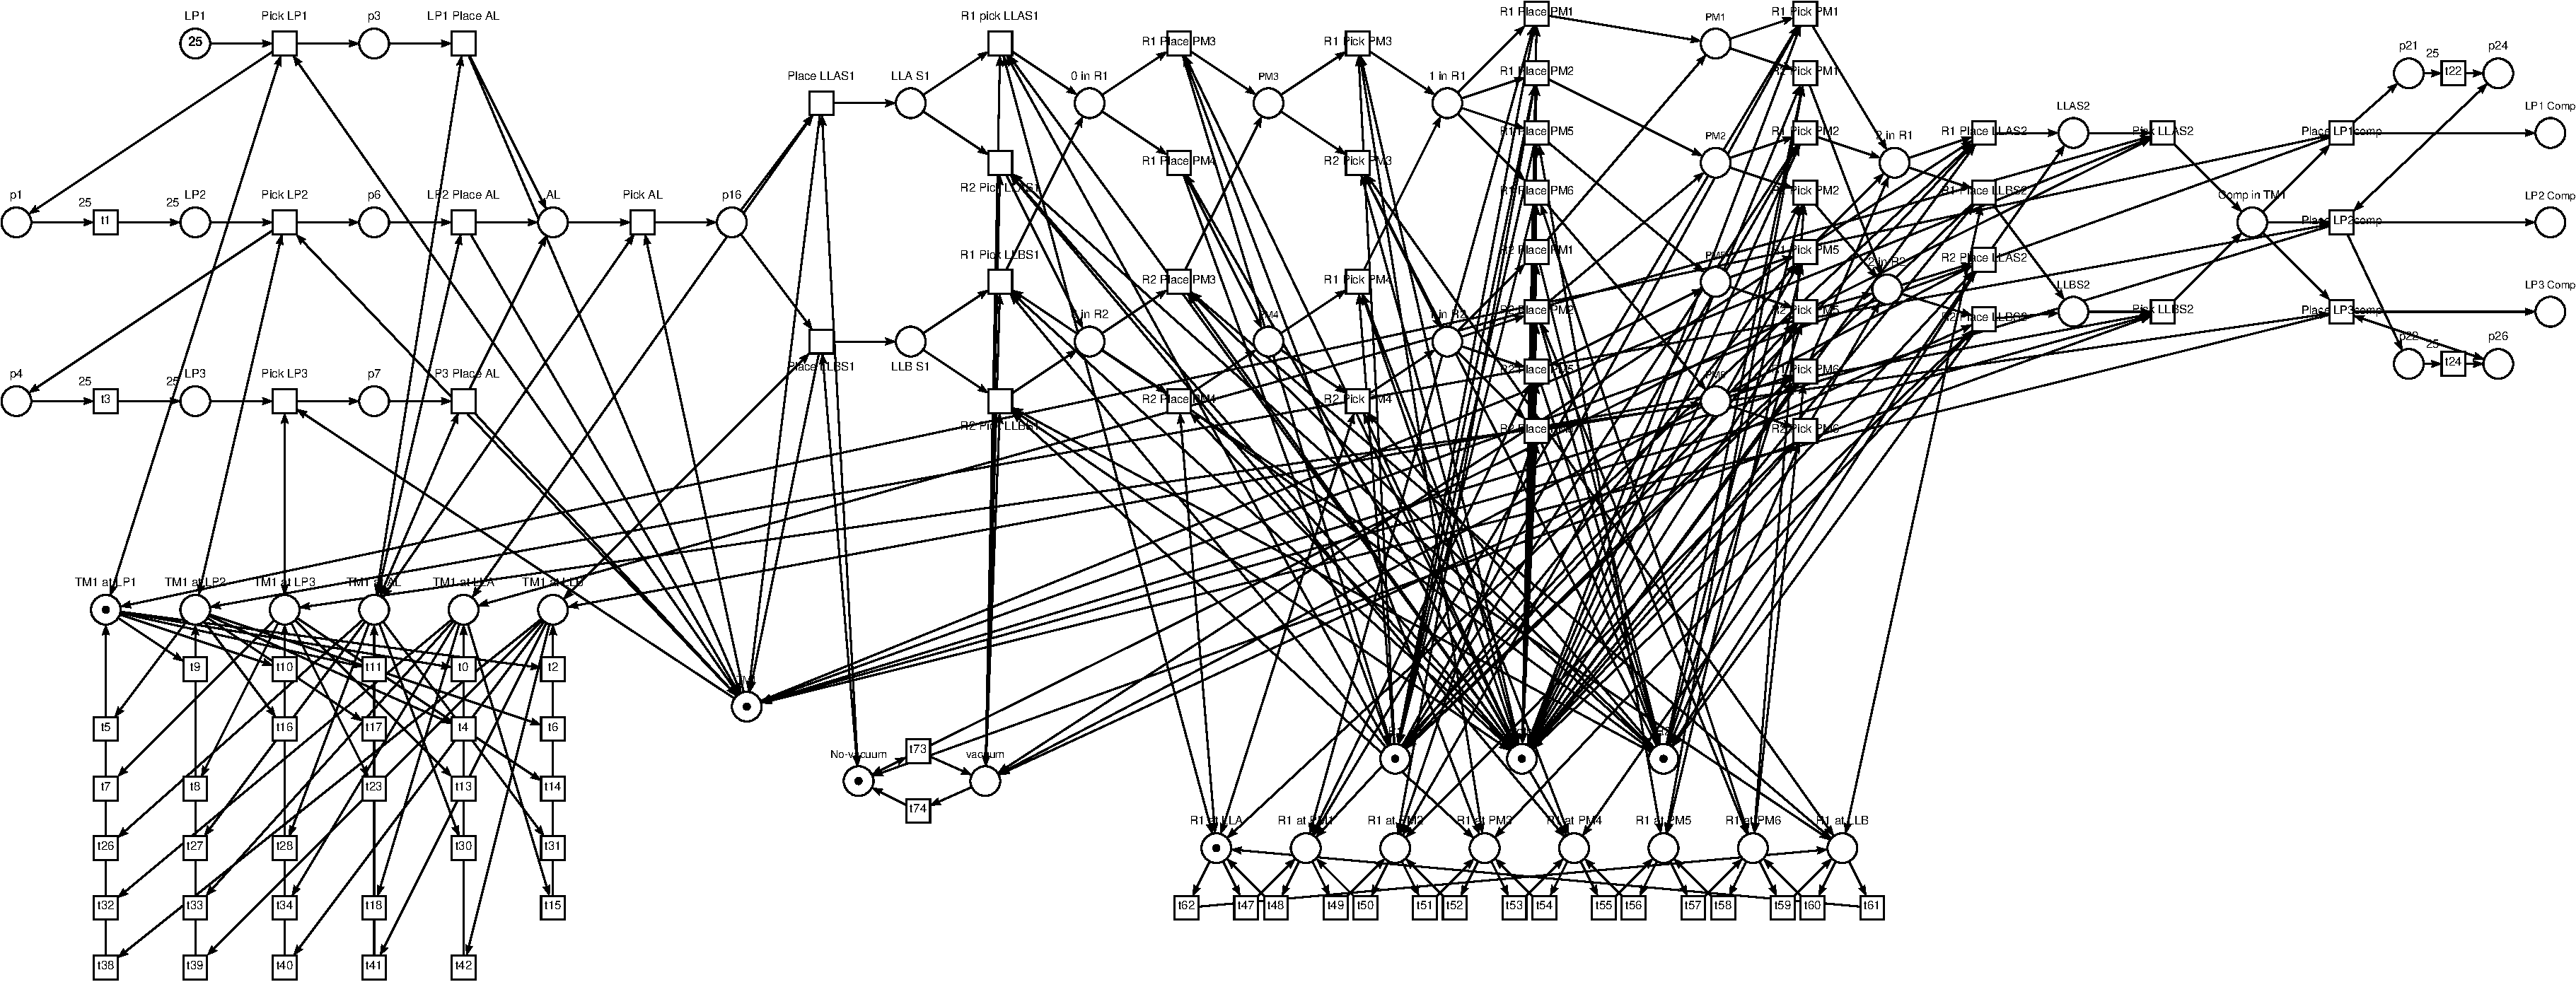
\includegraphics[width=\linewidth]{figures/国赛问题一完全.pdf}\\
	\caption{实际晶圆制造系统}
\end{figure}

本文第四章将使用蚁群算法对此模型进行调度。
\section{本章小结}
本章在上一章的基础上,将库所时间网和变迁时间网结合起来,提出了一种新的时间网子类:库所变迁时间网(TTPPN);
设计了一套TTPPN发射变迁的流程,供下一章的调度算法使用;
设计了一种计算各种Petri网模型的程序架构;
最后使用TTPPN对一个实际的晶圆制造系统进行建模。
% \chapter{基于库所变迁时延网的蚁群算法研究}
第二章介绍了一系列的时间Petri网,第三章提出了一种称为TTPPN的时间网子类,
并基于TTPPN对一个实际的半导体晶圆生产系统进行了建模。

本章将基于上章建立的TTPPN模型,使用算法计算出一条变迁序列。
TTPPN发射此变迁序列,会到达一个规定好的终止标识。
在实际的半导体晶圆生产系统中,最开始,晶圆会堆放在一个腔体中。
随着加工过程的运行,晶圆会被带离初始的腔体,经过一系列的环节,最终被放入到另一个腔体中。
在TTPPN中,这些腔体可被建模为库所。
因此算法的任务即为寻找一条能将一个库所中所有托肯转移到另一个库所中的变迁序列。

另外,按上一章的变迁发射逻辑,每个变迁发射都会有一个具体的时刻,将此时刻作为一个属性存入TTPPN的标识中,称为全局时刻。
TTPPN发射变迁序列生成的最终标识的全局时刻即为此系统完成晶圆加工的总耗时,称为完工时间。
实际情况下,需要完工时间越短越好。这个值将用来衡量算法的解质量。
算法从开始到找到终止标识所消耗的时间称为程序运行时间。这个值将用来衡量算法的速度。
对于启发式算法、群体智能算法来说,时间复杂度的分析十分困难。另外程序运行时间还会受操作系统进程调度策略的影响,未必能如实反映算法速度。
因此本章将记录Petri网的发射次数,用以作为分析算法速度的补充数据。
当Petri网的库所、变迁数确定时,发射变迁产生新标识的时间开销也是确定的。
而对于蚁群算法,其大部分时间开销是发射变迁带来的,因此用发射次数来表征算法的速度。
\section{基于TTPPN的基本蚁群算法}
蚁群算法(Ant Clony Optimization, ACO)是一种群智能算法,
它是由一群无智能或有轻微智能的个体(Agent)通过相互协作而表现出智能行为,
从而为求解复杂问题提供了一个新的可能性。
蚁群算法最早是由意大利学者Colorni A., Dorigo M. 等于1991年提出。
算法运行时蚂蚁会以更高的概率选择信息素浓度高的路,
而蚂蚁会为长度短的路留下更多的信息素。
因此选路机制与信息素添加机制构成了一个正反馈的逻辑,
随着程序的持续运行,正反馈会将解往更优的方向引导\cite{blum2003metaheuristics}\cite{li2015survey}\cite{colorni1992distributed}\cite{kennedy1995particle}\cite{dorigo2004ant}。

TTPPN为时间网,其托肯和变迁上均有时钟,
如果要完整的表示TTPPN,需要记录每一个托肯和变迁上的时钟。
即便两标识中所有库所中的托肯数都相同,但只要托肯上的时钟计时不同,
依然要视为不同的标识。
因此TTPPN与其不加时间的网相比,可达图会异常庞大。

但是在蚁群算法中,即便不存储TTPPN的完整信息,依然可以保证上述正反馈逻辑。
当区分标识仅考虑标识的库所向量时,可达图便可看作是一个边上权值可变的有向图。
\begin{figure}[H]
	\centering
	% Requires \usepackage{graphicx}
	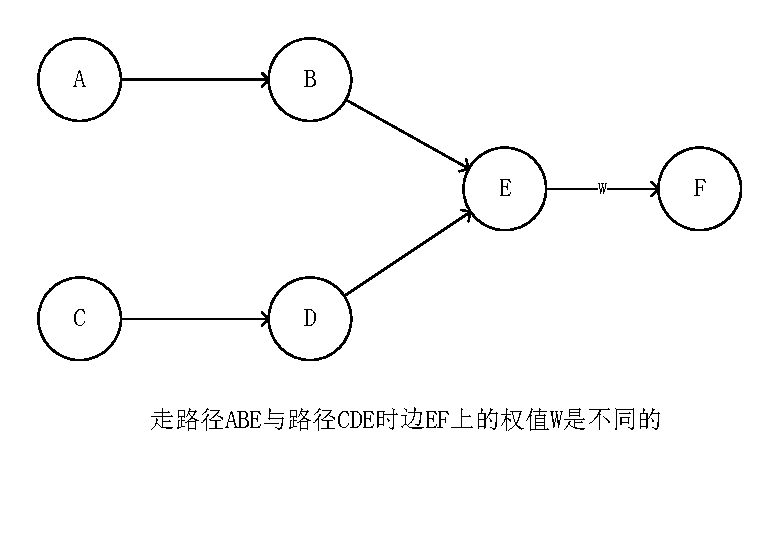
\includegraphics[scale=0.7,angle=0]{figures/可变权值图.pdf}\\
	\caption{可变权值图}
\end{figure}
边上权值会受到初始标识到此标识路径的影响。
选路机制与信息素添加机制构成的正反馈逻辑并不会被破坏,
因此即便不区分时钟计时不同的标识,依然可以使用蚁群算法。

基于TTPPN的基本蚁群算法可分为三个阶段:蚂蚁循迹阶段、信息素稀释阶段和信息素添加阶段。

\begin{algorithm}[H]
    \caption{基于TTPPN的基本蚁群算法}
    \hspace*{0.02in} {\bf 输入:} 
    变迁库所时间网$TTPPN$,变迁库所时间网的初始标识$initMarking$,蚂蚁只数$antCount$,算法迭代轮数$round$\\
    \hspace*{0.02in} {\bf 输出:}
	变迁序列$trans$
    \begin{algorithmic}[1]
		\For {$i \leftarrow 1, round$}
			\State $Ants \leftarrow$初始化$antCount$只蚂蚁放入蚂蚁集合
			\State $RG \leftarrow$初始化一个空的可达图
			\State $antsTravel(Ants,RG,TTPPN,initMarking)$ //蚂蚁循迹阶段
			\State $dilute(RG)$ //信息素稀释阶段
			\State $putPheromone(RG,Ants)$ //信息素添加阶段
		\EndFor
		\State 返回找到的最优变迁序列$trans$
    \end{algorithmic}
\end{algorithm}

蚂蚁循迹阶段是算法的主要流程,本阶段中每只蚂蚁都会独立地在可达图中进行搜索。

\begin{algorithm}[H]
	\caption{蚂蚁循迹阶段}
	\label{alg4-2}
	\begin{algorithmic}
		\Procedure {antsTravel}{$Ants$,$RG$,$TTPPN$,$initMarking$}
		\ForAll{$ant \in Ants$} //$Ants$为蚂蚁的集合
			\State $antTravel(ant,RG,TTPPN,initMarking)$ //单只蚂蚁循迹
		\EndFor
		\EndProcedure
	\end{algorithmic}
\end{algorithm}

每只蚂蚁都有一个禁忌表,蚂蚁每次会选择发射一个变迁,并把发射变迁生成的标识存入此禁忌表中,之后的搜索过程会禁止发射到禁忌表中已经有的标识,
避免蚂蚁走重复的路。
此蚂蚁共有两种结局:1、蚂蚁走到终点标识;2、蚂蚁无路可走。

\begin{algorithm}[H]
	\caption{单只蚂蚁循迹}
	\label{alg4-3}
	\begin{algorithmic}
		\Procedure {antTravel}{$ant$,$RG$}
		\State $tabu \leftarrow$ 初始化蚁群禁忌表
		\State $log \leftarrow$ 初始化蚂蚁日志
		\While {蚂蚁未到达终点并且未走到死路} 
			\State $next(ant,RG,TTPPN,initMarking,tabu,log)$ //为蚂蚁选择变迁并发射的逻辑
		\EndWhile
		\EndProcedure
	\end{algorithmic}
\end{algorithm}

蚂蚁无路可走既可能是因为蚂蚁走上了死锁标识,没有使能变迁可以发射,也可能是此标识的所有使能变迁发射后的标识均在禁忌表中出现过了。
蚂蚁会一直搜索下去直到走到终点,蚂蚁在搜索过程中会记录发射的变迁序列,用以更新可达图上的信息素和输出最后的解。
因为每只蚂蚁的搜索过程相互独立,所以每只蚂蚁搜索过程可由独立的线程并发执行,以提升效率。
蚁群算法的可达图是不带有时间信息的,仅由标识与标识通过使能变迁连接,标识为图的节点,变迁为图的有向弧。
变迁上有一个权值,称为信息素浓度,蚂蚁会根据信息素浓度,并综合考虑到禁忌表,随机选择一个使能变迁发射。
如果蚂蚁到达的标识之前未被添加进可达图,则默认这个标识的所有使能变迁上的信息素浓度是相同的。

\begin{algorithm}[H]
	\caption{蚂蚁选择变迁并发射的逻辑}
	\label{alg4-4}
	\begin{algorithmic}
		\Procedure {next}{$Ants$,$RG$,$TTPPN$,$initMarking$,$ant$,$RG$}
		\State $t=chose(RG,initMarking)$
		\State $initMarking=lanuch(TTPPN,initMarking,t)$
		\State 将当前标识添加进禁忌表$tabu$中
		\State 将发射的变迁$t$记录在蚂蚁日志$log$中
		\EndProcedure
	\end{algorithmic}
\end{algorithm}

\textbf{定义4.1}\textbf{:}
记$P_{Mt}$为可达图中标识$M$的变迁$t$上的信息素浓度,$P_{Mt}\in \mathbb{R}$。
处于标识$M$的蚂蚁选择发射变迁$t$的概率为
$
	\frac{P_{Mt}}{\sum_{i \in T} P_{Mi} }
$。
蚂蚁随机选择变迁发射的算法为轮盘赌算法。
如果有n个待选择的元素,此算法会生成n个彼此相邻的区间,区间的长度与此元素被选择的概率成正比。
算法会随机生成一个大于0,小于区间长度的数值。
这个数值落在哪个区间内,算法就会选择哪个数。

\begin{algorithm}[H]
	\caption{蚁群算法中的轮盘赌算法}
	\label{alg4-5}
	\begin{algorithmic}
		\Procedure {chose}{$RG$,$initMarking$}
		\State $total \leftarrow 0$
		\State $probability \leftarrow $ 用于存储变迁和变迁上信息素浓度的键值对集合
		\State 
		\ForAll{$t \in T$}
			\If{$t^{-} \le m$}
				\State $next \leftarrow lanuch(TTPPN,initMarking,t)$
				\If{$next \in tabu$}
					\State continue
				\EndIf
				\State $value \leftarrow$ 变迁$t$上的信息素浓度
				\State $total=total+value$
				\State $put(probability,t,value)$ //$put(probability,t,value)$指在键值对集合probability中添加键值对$(t,value)$
			\EndIf
		\EndFor
		\State $random \leftarrow $随机生成一个大于0,小于$total$的数
		\State $total=0$
		\ForAll{$t \in keys(probability)$} //$keys(probability)$表示键值对集合$probability$中键的集合
			\State $value \leftarrow get(probability,t)$ //$get(probability,t)$表示从键值对集合$probability$中取键$t$的值
			\State $total=total+value$
			\If{$total \ge random$}
				\State return true
			\EndIf
		\EndFor
		\EndProcedure
	\end{algorithmic}
\end{algorithm}

蚂蚁会根据可达图变迁上的信息素浓度的大小,随机选择一个变迁发射,并在走到终点后,为可达图增加信息素。
随着蚁群算法不断运行下去,可达图中的信息素浓度会越来越高,导致之后蚂蚁添加的信息素占总信息素浓度的比重越来越低。
在这种情况下,后期蚂蚁对解的影响将会减少。
而前期可达图中信息素尚少,蚂蚁循迹几乎是随机的,所以后期的蚂蚁比前期的蚂蚁更为重要。
因此应该加入信息素稀释机制。

\textbf{定义4.2}\textbf{:}
记$\alpha $为信息素稀释率,$\alpha \in \mathbb{R}$,$P_{Mt}^{i}$为蚁群算法第$i$轮中$P_{Mt}$的值。
记$A_{Mt}^{ji}$为第$j$只蚂蚁第$i$轮要在标识$m$上添加的信息素浓度。
$P_{Mt}^{i+1}=\alpha P_{Mt}^{i}+A_{Mt}^{ji}$

每轮可达图上的信息素都会按比例被稀释掉。
\begin{algorithm}[H]
	\caption{信息素稀释阶段}
	\label{alg4-6}
	\begin{algorithmic}
		\Procedure {dilute}{$RG$}
			\ForAll{$M \in RG$}
				\ForAll{$t \in T$}
					\State $P_{Mt}=\alpha P_{Mt}$
				\EndFor
			\EndFor
		\EndProcedure
	\end{algorithmic}
\end{algorithm}

蚁群在循迹过程中,会将到达终点标识的变迁标识序列保存起来,称为蚂蚁日志(log),并在添加信息素阶段根据蚂蚁日志,更新信息素。
如果蚂蚁日志中的标识已经在可达图中存在,则直接更新其上的信息素。
如果此标识之前从未被放入可达图,则在此时放入可达图。
因此蚁群算法的可达图是随着算法运行,逐渐扩展出来的,并不需要一开始就提供。
信息素的添加量要和路径长度成反比,在我们时间网的场景下,蚂蚁日志中的变迁标识序列中最后一个标识记录的时刻是完成调度的总耗时。
因此信息素的添加量应与这一时刻成反比。

\textbf{定义4.3}\textbf{:}
记$T_{ji}$为第$j$只蚂蚁第$i$日志的变迁标识序列中最后一个标识记录的时刻,此蚂蚁要在标识$m$上添加的信息素浓度$A_{Mt}^{ji}=\frac{C}{T_{ji}} $。

\begin{algorithm}[H]
	\caption{信息素添加阶段}
	\label{alg4-7}
	\begin{algorithmic}
		\Procedure {putPheromone}{$RG$,$Ants$}
			\ForAll{$ant \in Ants$}
				\ForAll{$M \in Markings(log)$} \\$Markings(log)$为蚂蚁日志log中的标识序列
					\If{$M \in RG$}
						\State $P_{Mt}=A_{Mt}$
					\Else
						\State 将$M$放入$RG$中
						\State $value \leftarrow 默认值$
						\State $P_{Mt}=value$
					\EndIf
				\EndFor
			\EndFor
		\EndProcedure
	\end{algorithmic}
\end{algorithm}
上述流程如果以单只蚂蚁为粒度,进行并发计算,无线程安全问题容易解决。
因为每只蚂蚁所需要的资源仅有两种:可达图、蚂蚁日志。
其中日志为每只蚂蚁私有资源,其他蚂蚁无权操作,因此无线程冲突。
而蚂蚁对于可达图有两种操作:读、写。
写操作只发生在稀释和更新信息素阶段。
而读操作发生在蚂蚁循迹阶段。
读写操作是分离的。
因此读操作不存在线程冲突。

对于写操作,有线程安全问题,因此需要加锁,并发度不如其他流程。
但通过合理选择可达图的数据结构,可以尽可能提升并发度。

\section{蚁群可达图使用的数据结构}
蚂蚁在循迹阶段,需从可达图上得出当前标识上各个使能变迁的信息素浓度。
因此蚂蚁对可达图有查询操作。

在信息素浓度稀释阶段,可达图上各个变迁的信息素浓度需按比例稀释。
因此可达图需支持修改数据的操作。

在添加信息素阶段,蚂蚁有可能探索到从未被发现的标识。
需要将这个标识的信息加入可达图中。
因此蚂蚁对可达图有添加信息的操作。

随着算法的一轮轮迭代,某些标识上的使能变迁的信息素已经被稀释到很低了。
蚂蚁走上此标识的概率极小,即便走上了,其使能变迁上信息素浓度也近乎均匀。
因此应该从可达图中删除这类标识,以节约内存。

基于以上的分析,蚁群算法的可达图需支持增、删、改、查四种操作。
所以应该选择增、删、改、查复杂度均为$O(1)$的哈希表作为数据结构实现。

可达图在算法流程中需写入数据,此操作有线程安全问题,因此需要对其加锁。
一下两种为哈希表的常规加锁方式。
\subsection{对操作方法加锁}
当算法中有线程要对可达图进行写入操作时,
需尝试取得写入操作的锁,
并在写入完成后释放锁。
锁的数量只有一个。
对于取得锁和释放锁的逻辑,均调用操作系统自带的原语以保证原子性。
如果某流程具有原子性,则此流程只有两种状态:未开始状态、已完成状态。
因此可以使用CAS原语实现加锁。
CAS的功能是将某地址的值与给定值比较并交换,并根据比较结果返回特定值。
CAS方法具有原子性,利用CAS方法的特点可以设计互斥锁。
互斥锁实现方法如下:

1、判断CAS操作是否成功,如果不是则重复此步;

2、执行写可达图的操作;

3、使用CAS将特定地址的值置回初值。


使用此逻辑,保证了不可能有两个线程同时修改可达图,从根本上解决了线程安全问题。
但是这种加锁逻辑,过于粗糙,大大降低了并发度。

使用CAS锁,如果某线程未取得锁,它会一直尝试取得锁。
可以使用信号量机制,直接让处理机暂停执行此线程,从而执行其他线程,来提高效率。
\subsection{对数据加锁}
即便是对可达图进行修改,如果修改的不是同一个标识的数据,也是不会有线程安全问题的。
而同时对同一个标识进行写操作,完全是小概率事件。
所以对具体标识进行加锁是更为高效的选择。

基于哈希表的底层原理,实际上是对哈希表内部数组的各个地址进行加锁,锁的数量最多为内部数组长度。
当写操作需要处理某地址的数据,先尝试取得此地址上的锁,并在写入完成后释放锁。

锁的数量增加会带来额外的内存开销。
如果需减少这部分的内存开销可以将锁加在地址的区间上,以减少锁的数量。
\section{备份可达图提高算法并发度}
本算法分为三个阶段:蚂蚁循迹阶段、信息素稀释阶段、信息素添加阶段。
原算法中三阶段是串行的。
蚂蚁需要先循迹,得到解后才能添加信息素,因此第一阶段和第三阶段存在依赖关系,必然是串行的。
然而第二阶段和一、三阶段的依赖关系并不明确。
理论上第二阶段和第三阶段可看作是一个大阶段,
即更新信息素阶段。
而第一阶段和第三阶段本质上并没有依赖关系,
只因为第一阶段蚂蚁循迹需要读可达图,第二阶段可达图稀释需要写可达图,
因此为保证线程安全,将其分为两个阶段。

如果将可达图备份一份,这两个阶段是可以并发执行的。

现将可达图分为两份,主可达图($RG$)与副可达图($RGCopy$)。
这两份可达图互为副本,在之后蚁群算法一轮轮迭代中会交替充当主可达图供蚁群使用。

在蚂蚁循迹阶段另外加入一个线程,专门用于完成可达图备份与稀释。

主可达图因为上一轮被修改了信息,这部分信息未被加入副可达图中,
副可达图也需要同步这部分修改。

修改的内容分为三部分:对原标识的信息素更新、添加新标识、删除信息素浓度过低的标识。
因此需遍历原可达图,并基于此修改副可达图的信息。
再遍历副可达图,删除原可达图中不存在的标识。

完成蚂蚁循迹流程后,交换原副可达图。

\begin{algorithm}[H]
	\caption{备份可达图}
	\label{alg4-9}
	\begin{algorithmic}
		\Procedure {copy}{$RG$,$RGCopy$}
			\ForAll{$m\in RG$}
				\If{$m \in RGCopy$}
					\State 同步$m$上的信息素浓度
				\Else
					\State 将$m$添加入$RGCopy$中
				\EndIf
			\EndFor
				\ForAll{$m \notin  RGCopy$}
				\If{$m \in RG$}
					\State 从$RGCopy$中删除$m$
				\EndIf
			\EndFor
		\EndProcedure
	\end{algorithmic}
\end{algorithm}

\section{蚁群求解实际问题}
本节将使用蚁群算法求解第四章对实际晶圆生成系统建立的模型。
为衡量蚁群算法解的质量,需要知道模型的最优调度策略。
本节将使用迪杰斯特拉算法求解Petri网模型的最优变迁序列。
\subsection{基于迪杰斯特拉算法求解Petri网最优变迁序列}
迪杰斯特拉算法用于求取图的最短路径。
如果图的节点数为n,此算法可以在$O(nlog(n))$的时间复杂度下得出各节点到起点的最短路径。

基于时间网的背景,设计迪杰斯特拉算法。

\subsubsection{存放将要扩展的标识的集合}
设计一个集合,此集合专门用于存放接下来将要扩展的标识,命名为$OPEN$集合。
Petri网的可达图是随算法运行动态添加进内存中的,所以$OPEN$中一开始只有初始标识,
随着程序的运行,如果遇到有扩展价值的标识,此标识会被放入$OPEN$中。

$OPEN$会被取出标识进行扩展,也会被放入标识。
但基于迪杰斯特拉算法的机制,取出的标识应该是集合中离原点最近的标识,
也就是全局时间最短的标识。

如果遍历这个集合寻找全局时间最短的标识,当集合大小为$n$时,其时间复杂度为$O(n)$。
但是如果使用小根堆去实现,其时间复杂度为$O(log(n))$。
因此本算法将使用小根堆作为此集合的实现。

\subsubsection{已经扩展的标识的集合}
此集合专门用于存放已经扩展的标识,命名为$CLOSE$集合。
当一个标识从$OPEN$取出,并且它的所有变迁均被处理过,就会放入此集合中。
因为每次处理的标识都是$OPEN$中全局时间最短的标识,
所以当此标识进入$CLOSE$中,如果之后再扩展到它,如果时间网可达图路径上的时间间隔是确定的,其全局时间必然更长。
所以当标识已经在$CLOSE$中了,是没有扩展的意义的。

但实际上时间网可达图路径上的权值是可变的,所以$CLOSE$表中存储的为键值对,键为标识,值为目前到达此标识的最短时间。
此后判断标识是否值得扩展,应该判断到达此标识的全局时间是否比$CLOSE$表中记录的最短时间短,
如果此时间确实更短,才去扩展此标识。

$CLOSE$涉及到两种操作:将已完成扩展的标识存入此集合中、查询标识是否在此集合中。
因此本算法选取哈希表作为此集合的数据结构实现。哈希表存与查的时间复杂度均为$O(1)$。
使用哈希表实现的$CLOSE$其底层是一个固定长度的数组。
标识需要得到$CLOSE$底层数组的一个元素索引,才能进入$CLOSE$表。
进入$CLOSE$表的标识会被存放在特定索引上。
此索引是根据哈希值得出的,哈希值是使用哈希函数得出的,哈希函数的输入是标识向量。
对于哈希值相同的标识,本$CLOSE$表会将其统一存放在一棵红黑树中。
如果红黑树的节点数为$n$,其增删改查的时间复杂度是$log(n)$。

\subsection{算法流程}
迪杰斯特拉算法每次会从$CLOSE$中取一个全局时间最短的标识$curr$,如果此标识就是终点标识,则找到终点。
如果$CLOSE$集合取空都未找到终点,则说明终点不可达。
对$curr$的所有使能变迁均发射一次,如果发射产生的新标识$next$已经在$OPEN$中存在,并且其全局时间更短,则将其取出,更新其全局时间后再放入。
在$OPEN$中查询标识的时间复杂度为$O(log(n))$,往其放入标识的时间复杂度为$O(log(n))$。
如果$next$的全局时间已经高于$CLOSE$中对于标识处记录的最短时间,则没有必要扩展此标识,如果不存在,之前查找时也没在$OPEN$中找到就将此标识放入$OPEN$中。
当$curr$的所有使能变迁均处理完成,将其放入$CLOSE$中。

迪杰斯特拉算法流程如下所示:

\begin{algorithm}[H]
    \caption{基于时间网的迪杰斯特拉算法}
    \hspace*{0.02in} {\bf 输入:} 
    变迁库所时间网$TTPPN$,变迁库所时间网的初始标识$initMarking$,终点标识$endMarking$\\
    \hspace*{0.02in} {\bf 输出:}
	变迁序列$trans$
    \begin{algorithmic}[1]
		\For {$i \leftarrow 1, round$}
			\State 往$OPEN$放入初始标识$initMarking$
			\While{$OPEN$不为空}
				\State $curr \leftarrow$从$OPEN$中取出全局时间最小的标识
				\ForAll{$t\in curr$的使能变迁}
					\State $next \leftarrow launch(TTPPN,curr,t)$
					\If{$next$在$OPEN$中且全局时间更短}
						\State 更新$OPEN$中$next$的全局时间
					\EndIf
					\If{$next$值得扩展}
					\State 将$next$放入$OPEN$
					\EndIf
				\EndFor
				\State 将$curr$放入$CLOSE$中
			\EndWhile
		\EndFor
		\State 返回找到的最优变迁序列$trans$
    \end{algorithmic}
\end{algorithm}

\subsection{实验和结果分析}
在处理器为i5-1130G7,最大内存为8GB的设备上,排除文件读入、结果输出的耗时,仅在调用算法前后记录系统时间戳,
分别使用迪杰斯特拉算法和蚁群算法求解第五章建立的晶圆制造系统的模型。

\subsubsection{迪杰斯特拉算法的实验结果分析}
以下是使用6GB内存,迪杰斯特拉算法的结果。

变迁序列为:$t_{1}$->$t_{7}$->$t_{1}$->$t_{2}$->$t_{1}$->$t_{17}$->$t_{3}$->$t_{7}$->$t_{16}$->$t_{1}$->$t_{23}$->$t_{2}$->$t_{1}$->$t_{17}$->
$t_{27}$->$t_{7}$->$t_{16}$->	$t_{1}$->$t_{2}$->$t_{1}$->$t_{4}$->$t_{14}$->$t_{24}$->$t_{12}$->$t_{22}$->$t_{1}$->
$t_{13}$->$t_{29}$->$t_{11}$->$t_{22}$->$t_{1}$->$t_{14}$->$t_{12}$->$t_{22}$->$t_{20}$->$t_{18}$->$t_{1}$->$t_{4}$->$t_{14}$->
$t_{24}$->$t_{12}$->$t_{22}$->$t_{20}$->$t_{18}$->$t_{13}$->$t_{1}$->$t_{29}$->$t_{11}$->$t_{22}$->$t_{20}$->$t_{18}$->$t_{14}$->
$t_{1}$->$t_{12}$->$t_{22}$->$t_{20}$->$t_{18}$->$t_{1}$->$t_{4}$->$t_{14}$->$t_{24}$->$t_{12}$->$t_{22}$->$t_{20}$->$t_{18}$->
$t_{13}$->$t_{20}$->$t_{18}$->$t_{8}$->$t_{29}$->$t_{22}$->$t_{14}$->$t_{20}$->$t_{18}$->$t_{9}$->$t_{22}$->$t_{20}$->$t_{18}$->
$t_{20}$->$t_{18}$->$t_{4}$->$t_{10}$->$t_{9}$->$t_{24}$->$t_{22}$->$t_{6}$->$t_{8}$->$t_{22}$->$t_{28}$->$t_{10}$->$t_{20}$->
$t_{18}$->$t_{9}$->$t_{22}$->$t_{20}$->$t_{18}$->$t_{20}$->$t_{18}$->$t_{4}$->$t_{10}$->$t_{9}$->$t_{22}$->$t_{20}$->$t_{18}$

完工时间为:1600.8s

程序运行时间为:8.972s

迪杰斯特拉算法每次都会选取离起点最近的节点进行扩展,因此扩展过程为一层层推进,其扩展过的可达标识数与可达图成比例。
本算法在使用变迁发射方法$launch$时会使用到标识的时钟信息,
而时间网的标识数巨大,为节约内存开销,本算法仅将标识向量存入$CLOSE$中。
因此在扩展过程中会产生大量的垃圾信息,需要被垃圾回收。
内存大小影响垃圾回收的次数,内存越大,垃圾回收次数越少。

分别测试从1GB内存到6GB内存迪杰斯特拉算法的程序运行时间。

\begin{table}[H]
	\centering
	\caption{内存与程序运行时间关系}
	\resizebox{!}{!}{
		\begin{tabular}{l|lllllllll}
			\toprule
			内存(GB) & 1 & 2 & 3 & 4 & 5 & 6 \\ \hline
			程序运行时间(s) & 12.695 & 10.930 & 9.031 & 8.752 & 8.803 & 8.972 \\
			\bottomrule
		\end{tabular}
	}
\end{table}

\begin{figure}[H]
	\centering
	% Requires \usepackage{graphicx}
	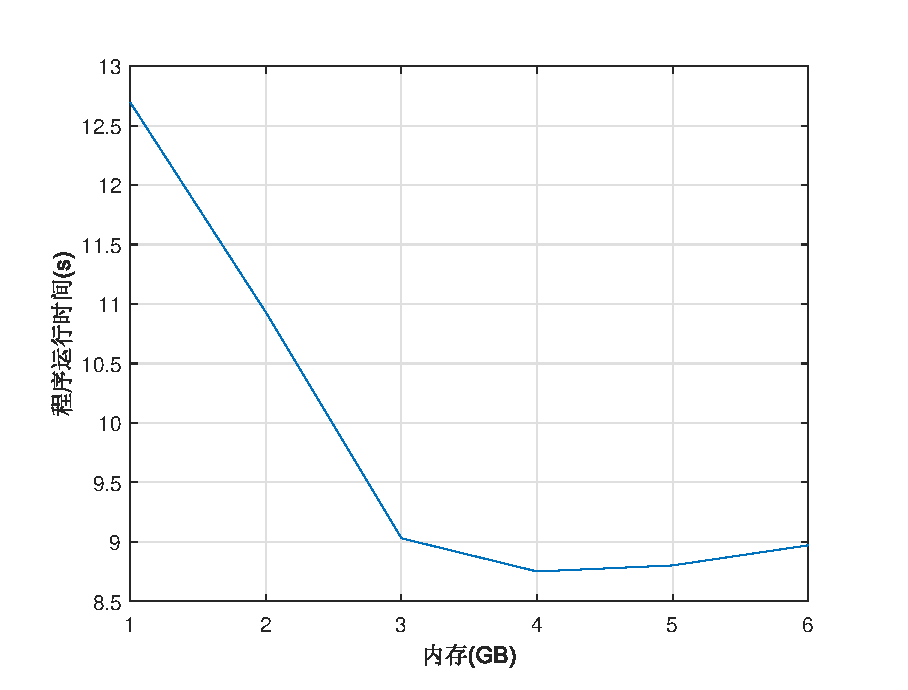
\includegraphics[scale=1.00,angle=0]{figures/mem_t.eps}\\
	\caption{迪杰斯特拉算法内存与程序运行时间关系}
\end{figure}

如上图所示,随着内存的增加,程序运行时间有下降的趋势,当内存增加到3GB时,程序运行时间稳定在9s左右。

\subsubsection{蚁群算法的实验结果分析}
以下是使用6GB内存,蚁群算法100只蚂蚁迭代100轮的结果。

变迁序列:$t_{1}$->$t_{2}$->$t_{1}$->$t_{7}$->$t_{17}$->$t_{3}$->$t_{16}$->$t_{23}$->$t_{1}$->$t_{2}$->$t_{1}$->$t_{4}$->$t_{13}$->$t_{24}$->$t_{7}$->$t_{14}$->$t_{3}$->$t_{4}$->$t_{9}$->$t_{10}$->$t_{24}$->$t_{22}$->$t_{1}$->$t_{11}$->$t_{13}$->$t_{23}$->$t_{21}$->$t_{19}$->$t_{12}$->$t_{21}$->$t_{18}$->$t_{17}$->$t_{20}$->$t_{18}$->$t_{1}$->$t_{27}$->$t_{24}$->$t_{10}$->$t_{28}$->$t_{12}$->$t_{14}$->$t_{23}$->$t_{22}$->$t_{8}$->$t_{21}$->$t_{24}$->$t_{6}$->$t_{19}$->$t_{12}$->$t_{22}$->$t_{17}$->$t_{8}$->$t_{27}$->$t_{22}$->$t_{1}$->$t_{7}$->$t_{1}$->$t_{17}$->$t_{7}$->$t_{20}$->$t_{18}$->$t_{23}$->$t_{1}$->$t_{2}$->$t_{1}$->$t_{17}$->$t_{7}$->$t_{20}$->$t_{19}$->$t_{3}$->$t_{28}$->$t_{14}$->$t_{27}$->$t_{12}$->$t_{21}$->$t_{16}$->$t_{18}$->$t_{24}$->$t_{14}$->$t_{4}$->$t_{9}$->$t_{21}$->$t_{18}$->$t_{6}$->$t_{28}$->$t_{8}$->$t_{6}$->$t_{24}$->$t_{10}$->$t_{22}$->$t_{4}$->$t_{9}$->$t_{10}$->$t_{21}$->$t_{18}$->$t_{9}$->$t_{22}$->$t_{20}$->$t_{18}$->$t_{8}$->$t_{21}$->$t_{18}$->$t_{20}$->$t_{18}$->$t_{20}$->$t_{18}$

完工时间:2554.7s

程序运行时间:23.374s

此结果无论是完工时间还是程序运行时间,均要长于迪杰斯特拉算法的解。

导致此结果的可能原因有3个:算法不能收敛、算法收敛到较差解、算法收敛慢。

基于以上的分析,设计实验。
依次提高迭代轮数,观察完工时间,如果随迭代轮数增加,完工时间分布随机,则说明算法未收敛。
如果随迭代轮数增加,完工时间区域稳定值,并且稳定值接近迪杰斯特拉算法的解,说明算法收敛慢,如果稳定值显著高于迪杰斯特拉的解,
说明算法收敛到较差解。

另外,在计算机CPU有限的情况下,提高蚂蚁只数会时程序频繁进行线程切换,增大程序运行时间。
使用需要探寻蚂蚁只数与算法效率的关系。

将迭代轮数从10轮每次递增10轮直到100轮,统计完工时间,观察蚁群算法是否有收敛趋势。

\begin{table}[H]
	\centering
	\caption{蚁群算法迭代轮数与完工时间的关系}
	\resizebox{\linewidth}{!}{
		\begin{tabular}{l|lllllllllllll}
			\toprule
				轮数 & 10 & 20 & 30 & 40 & 50 & 60 & 70 & 80 & 90 & 100 \\ 
				\hline
				完工时间(s) & 2554.7 & 2254.1 & 1956.1 & 1921.7 & 2223.8 & 2494.7 & 2513.5 & 2487.9 & 2393.8 & 2554.7 \\
				\bottomrule
			\end{tabular}
	}
\end{table}

如图所示,蚁群算法在本场景下并没有收敛,迭代轮数在30轮之前,完工时间有下降趋势,但随着轮数的增加,完工时间也增加,最终有稳定在2500.0s的趋势。

从这个结果可以看出,此蚁群算法收敛到一个较差的解上,而且并不是收敛到局部最优解,因为随着迭代轮数增加,算法曾到达了较优的解,但依然有向差解接近的趋势。

为证明前30轮确实有下降趋势,而非是偶然现象,将迭代轮数从1轮每次递增10轮直到10轮,统计完工时间。

\begin{table}[H]
	\centering
	\caption{蚁群算法迭代轮数与完工时间的关系(小轮数)}
	\resizebox{\linewidth}{!}{
		\begin{tabular}{l|lllllllllllll}
			\toprule
			轮数 & 1 & 2 & 3 & 4 & 5 & 6 & 7 & 8 & 9 & 10 \\ \hline
			完工时间(s) & 3274.6 & 3136.1 & 3153.8 & 3024.6 & 2952.2 & 2840.0 & 2708.3 & 2630.0 & 2600.5 & 2554.7 \\
			\bottomrule
		\end{tabular}
	}
\end{table}

\begin{figure}[H]
	\centering
	% Requires \usepackage{graphicx}
	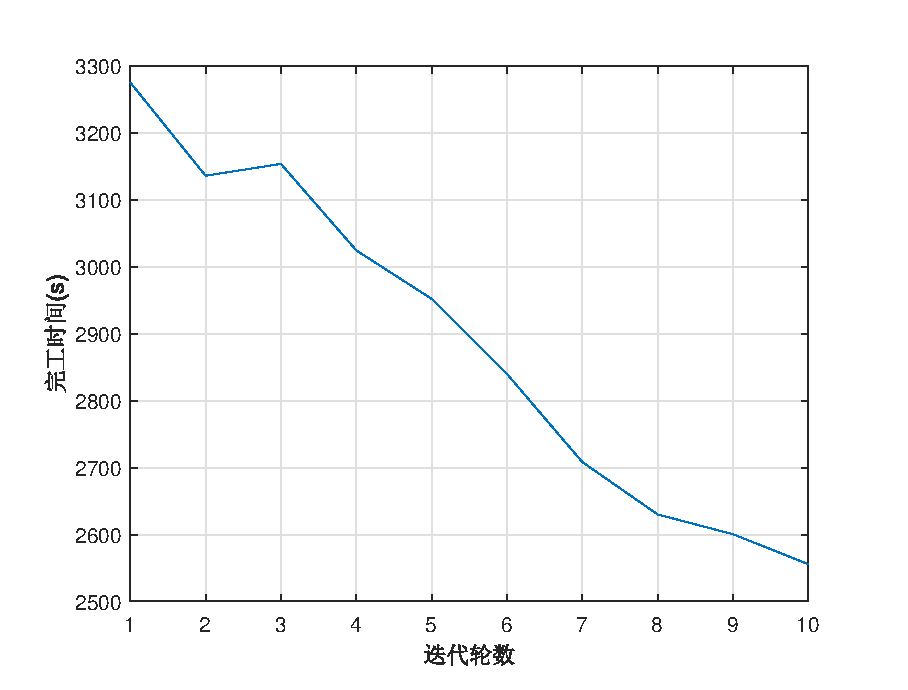
\includegraphics[scale=1.00,angle=0]{figures/round_t_small.eps}\\
	\caption{蚁群算法迭代轮数与完工时间关系(1到10轮)}
\end{figure}

如上图所示,低轮数时蚁群算法确实有收敛趋势。

本程序中每只蚂蚁都是一个线程,如果线程数量小于CPU数量,各个线程能并行指向,彼此互不影响。
而如果线程数量高于CPU数量,CPU就需要不断第切换到不同的线程,以实现程序并发地执行。
如果两线程竞争一个CPU,必然会导致其中一个线程等待。
因此随蚂蚁只数增加,程序运行时间会增加。
此外线程切换本身也是有开销的。
所以需要探寻蚁群算法蚂蚁只数对完工时间的影响,得出一个恰当的蚂蚁只数,并以此合理配置CPU数量。

为了观察蚂蚁只数对算法收敛性的影响,固定迭代轮数为10轮,从10只蚂蚁每次递增10只直到100只对此模型进行求解,观察完工时间。

\begin{table}[H]
	\centering
	\caption{蚁群算法蚂蚁只数与完工时间的关系}
	\resizebox{\linewidth}{!}{
		\begin{tabular}{l|lllllllllllll}
			\toprule
				蚂蚁只数 & 10 & 20 & 30 & 40 & 50 & 60 & 70 & 80 & 90 & 100 \\ \hline
				完工时间(s) & 2799.9 & 2404.6 & 3184.9 & 2314.9 & 2637.2 & 2718.6 & 2599.7 & 2596.0 & 2894.7 & 2554.7 \\
			\bottomrule	
		\end{tabular}
	}
\end{table}

\begin{figure}[H]
	\centering
	% Requires \usepackage{graphicx}
	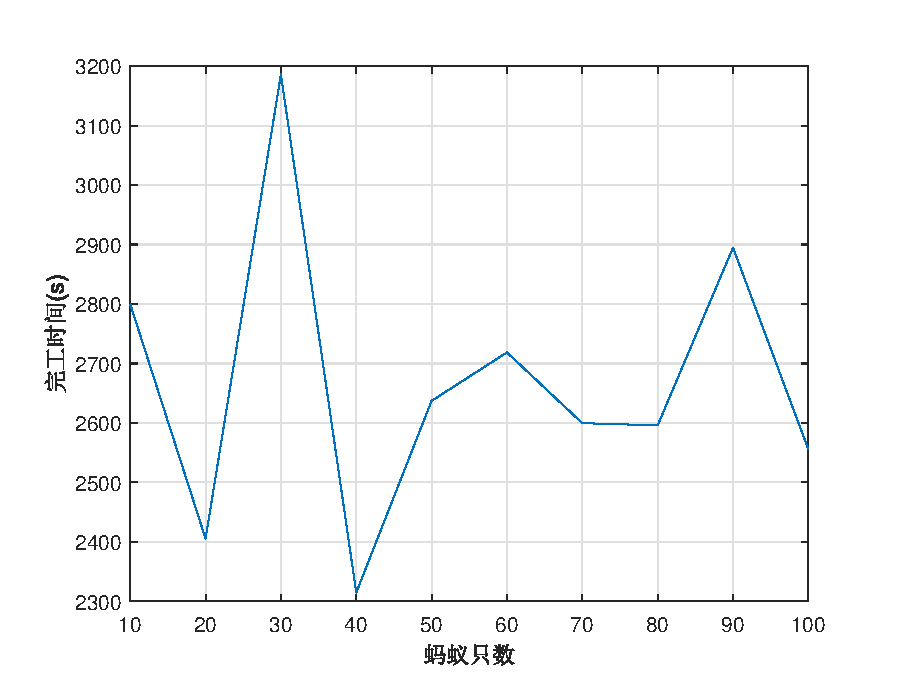
\includegraphics[scale=1.00,angle=0]{figures/count_t.eps}\\
	\caption{蚁群算法迭代轮数与完工时间关系(1到10轮)}
\end{figure}

如上图所示,随着蚂蚁只数的增加,完工时间是随机的,这意味着可能10只蚂蚁以后,蚂蚁只数就对算法收敛性影响不大了。

为表明低蚂蚁只数时,蚂蚁只数对算法收敛是有影响的,固定迭代轮数为10轮,从1只蚂蚁每次递增1只直到10只对此模型进行求解,观察完工时间。

如果蚂蚁只数在增加到一定值后,对解质量影响不大,则应该让蚁群算法运行在CPU数量高于此蚂蚁只数的机器上,
以避免线程切换与等待的开销,提升算法运行效率。

但是如果蚂蚁只数较高,应该选择处理器更多的GPU来运行蚁群算法。
本蚁群算法的可达图是动态扩展的,因此存在大量内存申请与清理的操作,此操作不适合在GPU上使用,
所以本文的代码是为CPU编写的。

\begin{table}[H]
	\centering
	\caption{蚁群算法蚂蚁只数与完工时间的关系(小只数)}
	\resizebox{\linewidth}{!}{
		\begin{tabular}{l|lllllllllllll}
			\toprule
			蚂蚁只数 & 1 & 2 & 3 & 4 & 5 & 6 & 7 & 8 & 9 & 10 \\ \hline
			完工时间(s) & 3640.5 & 3760.5 & 3262.0 & 3362.1 & 3256.0 & 3008.7 & 2651.0 & 2684.5 & 2752.9 & 2799.9 \\
			\bottomrule	
		\end{tabular}
	}
\end{table}

\begin{figure}[H]
	\centering
	% Requires \usepackage{graphicx}
	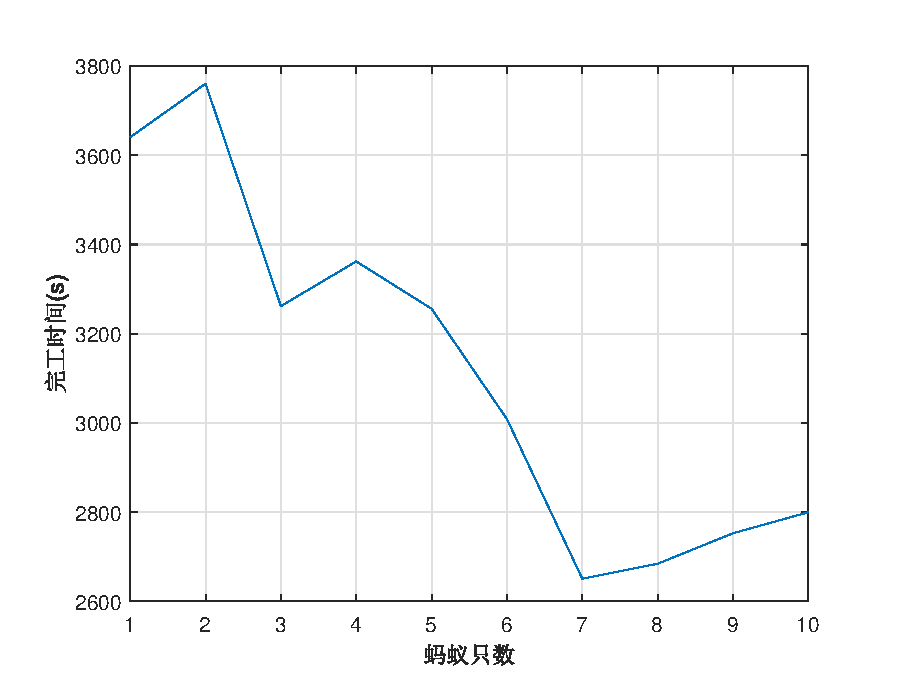
\includegraphics[scale=1.00,angle=0]{figures/count_t_small.eps}\\
	\caption{蚁群算法迭代轮数与完工时间关系(1到10轮)}
\end{figure}

如上图所示,在蚂蚁数量较少时,蚂蚁只数越大,完工时间越小。

综上,提升蚁群算法蚂蚁只数、和算法迭代次数,在一开始会对算法收敛性有较大贡献。随着蚂蚁只数增加到10只后,再增加蚂蚁只数对算法影响不大。
当迭代轮数增加到30轮以后,蚁群算法的解有恶化的趋势,再继续增加迭代轮数会使算法稳定在一个较差的解。

但是无论如何配置蚂蚁只数和迭代轮数,都无法使解向迪杰斯特拉算法求出的解靠近。下一节将继续分析蚁群算法解的情况,并且尝试了一系列优化方案。
\section{改进的蚁群算法}
基于上一小节的数据进行分析,原始的蚁群算法存在求解特定时间网的变迁序列时存在缺陷。
如果某时间Petri网的最优变迁序列上的使能变迁很少,
而完工时间较差的变迁序列彼此又互相连通,
原始蚁群算法便无法收敛。
其原因为走上最优解的蚂蚁有更高的概率走入死锁标识,失去添加信息素的资格。
而走向较差解的蚂蚁会有更高的概率走向终点标识,并在可达图上留下信息素。
原始蚁群算法的正反馈机制被打破,使算法无法收敛。
为修复这一异常,本文对原始蚁群算法进行了如下改进。
\subsection{超级蚂蚁机制}
如果此蚂蚁的解比目前的最优解还优,则赋予它添加更多信息素的权利,能添加的额外的信
息素和对解优化的贡献相关。
这么做是为了削弱之前非最优解的蚂蚁对流程的影响。当某蚂蚁运气好,得出的解远好于目
前的解,便可迅速提升这个解上的信息素,从而将误入歧途的蚂蚁重新引入正轨。

\textbf{定义4.5}\textbf{:}
记$MinTime$为蚁群算法运行时,当前得到的最短完工时间。
$CurrTime$为当前蚂蚁完成循迹后得出的完工时间。
$\beta$为此蚂蚁添加信息素的增益。
\begin{equation}
	\beta=\left\{
		\begin{aligned}
			1 \quad MinTime-CurrTime \leqslant 0\\
			MinTime-CurrTime \quad MinTime-CurrTime > 0\\
		\end{aligned}
		\right.
		\nonumber 
\end{equation}
此蚂蚁添加的信息素应乘上此增益。
因此第$j$只蚂蚁第$i$轮要在标识$m$上添加的信息素浓度$A_{Mt}^{ji}$应修改为
$$
A_{Mt}^{ji}=\beta A_{Mt}^{ji}
$$
当此蚂蚁循迹得出的解好于目前找到的最优解,它添加的信息素会被增益$\beta$放大。
当得出的解的完工时间越短,增益越大。
蚁群算法出现局部收敛时,
使用此机制,蚂蚁只要以小概率探索到了局部以外的更优解,
此解便会被添加大量信息素,
引导其他蚂蚁探索新解,
跳出局部收敛。

此蚂蚁需将找到的解更新为新的最优解。
因此在每只蚂蚁的添加信息素逻辑中需添加一段更新最优解流程。
\begin{algorithm}[H]
	\caption{更新最优解}
	\label{alg4-10}
	\begin{algorithmic}
		\Procedure {renNewMinTime}{}
			\If{$\beta>1$}
			\State $MinTime=CurrTime$
			\EndIf
		\EndProcedure
	\end{algorithmic}
\end{algorithm}

此流程中需修改$MinTime$这一全局变量。
而添加信息素逻辑是并发执行的,因此此处$MinTime$有可能同时被多个线程写入。
但因为此处即便有线程安全问题,也不影响算法执行,因此为提高并发度,不进行加锁。
\subsection{贪心选取初始信息素}
原算法蚂蚁遇到从未走过的地点(没有一只蚂蚁去过的地点),会以平均的概率选取下一步。
如果蚂蚁所在标识的各使能变迁是等价的,并不知道哪个变迁更优,蚂蚁在首次经过此标识时确实应该以平均的概率选择一条变迁。
但结合实际背景,这些变迁并不等价。
加工腔中的晶圆如果加工完毕,应该尽早取走。
基于此特点,
现将蚂蚁初次选路的策略修改为以更大的概率选择近的路。

将原算法中遇到新标识时构建新信息素对象的逻辑修改为以下逻辑。
\begin{algorithm}[H]
	\caption{贪心选取初始信息素}
	\label{alg4-11}
	\begin{algorithmic}
		\Procedure {greedyInitPheromone}{}
			\ForAll{$t\in T$}
				\If{$t^{-} \le m$}
					\State $nextMarking \leftarrow lanuch(currMarking,t)$
					\State 将变迁$t$上的信息素浓度设置为$time(nextMarking)-time(currMarking)$
					\\$time(marking)$为取得标识$marking$全局时间的方法
				\EndIf
			\EndFor
		\EndProcedure
	\end{algorithmic}
\end{algorithm}
对于此标识的所有使能变迁,均发射一次得出此标识的后继标识。
按这些后继标识的全局时间对这些变迁分配初始信息素。
时间越短初始信息素浓度越高。

这是一种贪心的思想。
发射使后继标识全局时间最短的变迁,意味着寻求单步最优的变迁发射。
实际生产系统中单步最优构成的解往往质量不差,因此这种逻辑在某些场景下,效果不错。
但如果模型最优解远离贪心解,此机制探寻新路径时依然会使用贪心的逻辑,会影响算法的收敛效率。
因此下一节将提出一种约束较弱的贪心策略。
\subsection{使用贪心算法预添加信息素}
与上一节使用的思想类似,使用贪心的思想优化算法。
具体逻辑为:
先使用贪心算法求解出一个解,在此解的变迁标识序列上添加一部分信息素。
再使用蚁群算法在此基础上继续求解。

贪心算法会不断地发射使后继标识全局时间最短的变迁,直到找到终点。
因为可达图中存在死锁标识,需为算法加入回溯机制,
遇到死锁标识时,回溯,并发射使后继标识的全局时间次大的变迁。

因此定义一个函数$find(marking)$,
此函数的功能为判断以标识$marking$为初始标识,判断是否能探索到与终点标识连通的路径。
\begin{algorithm}[H]
	\caption{贪心算法}
	\label{alg4-12}
	\begin{algorithmic}
		\Procedure {find}{$marking$}
			\If{$marking$为终点标识}
				\State return true
			\EndIf
			\State 对$marking$的使能变迁按全局时间进行排序,并装入$enableTrans$中
			\ForAll{$t \in enableTrans$}
				\State $nextMarking \leftarrow lanuch(t,currMarking)$
				\If{$nextMarking$被扩展过}
					\State continue
				\EndIf
				\If{$find(nextMarking)$}
					\State return true
				\EndIf
			\EndFor
			\State return false
		\EndProcedure
	\end{algorithmic}
\end{algorithm}
此函数使用递归实现了回溯功能。

在函数运行时一并记录发射的变迁,如果发生回溯,删除回溯的变迁,便得到一条变迁序列。
基于此序列预先为可达图分配信息素。

\subsection{复活蚂蚁}
当蚂蚁走到死锁标识时循迹结束,此时得到的变迁序列并不能到达终点标识,因此无法基于此序列添加信息素。
如果最优解附近存在大量死锁,那么大部分最优解附近的蚂蚁将失去添加信息素的资格,反而使得差解信息素浓度过高。
本节设计了一种机制,可以为使走上死锁的蚂蚁复活。

\textbf{定义4.6}\textbf{:}
记$similarity(s_{1},s_{2})$为标识序列$s_{1},s_{2}$的相似度。\\
$sameMarkingCount(s_{1},s_{2})$为标识序列$s_{1},s_{2}$中相同标识的数量。
$length(s_{1})$为$s_{1}$中标识的数量。\\
计算方法为:
$$
	similarity(s_{1},s_{2})=\frac{sameMarkingCount(s_{1},s_{2})}{length(s_{1})} 
$$

如果此蚂蚁死亡,则将其替换为活蚂蚁中与其相似度最高的蚂蚁。
\subsection{蚁群算法与模拟退火算法结合}
如果蚁群算法真的如预期,应该是会随着迭代次数的增加,收敛到一个最优解。这意味着最
优解实际上是出现在后期的。因此前期解的重要性不如后期。尽管本蚁群算法每轮都会去稀释信息素,但是是对信息素浓度总体进行成比例稀释。而信息素浓度分为两部分:初始信息
素+添加信息素。在前期解的重要性较弱的情况下,应该让蚂蚁更为随机地选择路径。所以前期应该降低添加信息素所占比例。
基于此思路,设计模拟退火机制:对添加信息素添加限制,随着轮数增加,逐步放开此限制。

\textbf{定义4.6}\textbf{:}
记$\varepsilon $为蚂蚁添加信息素的增益,
$i$为蚁群算法当前迭代轮数,
$round$为蚁群算法的总轮数。
$$
	\varepsilon=\frac{i}{round}
$$
将第$j$只蚂蚁第$i$轮要在标识$m$上添加的信息素浓度$A_{Mt}^{ji}$应修改为
$$
A_{Mt}^{ji}=\varepsilon A_{Mt}^{ji}
$$
随着轮数增加,增益$\varepsilon $会逐渐增加,加大了后期蚂蚁的重要性。

先前代码中为了加速收敛,提升了对解有贡献蚂蚁的地位。
这种蚂蚁出现在前期会让期待解变得很苛刻,以至于后期难有蚂蚁成为对解有贡献蚂蚁。
而模拟退火机制会削弱前期蚂蚁的地位。
两种机制实际上是矛盾的。

\subsection{蚂蚁回溯}
基于对本测试用例的解的分析,未避免走上最优解的蚂蚁重新走上岔路而死亡,
最为直观的策略为使蚂蚁拥有回溯的功能。
直接添加回溯功能会使蚂蚁不能死去,
以至于所有蚂蚁都要等待最后一只蚂蚁走到终点才能进行添加信息素的流程。
这无疑会极大地增加算法的时间开销。
所以应该设置蚂蚁寿命上限,
来提前结束对解优化意义不大的蚂蚁流程。
基于以上的分析,此寿命上限理应是当前最优解的全局时间。
但如果使用全局时间,
意味着其他蚂蚁依然会搜索以此全局时间为半径的部分可达图,
时间复杂度过大。
所以本算法倾向于使用最长跳数为蚂蚁寿命上限。

在原蚁群算法当蚂蚁循迹时,所有的后继标识均已在禁忌表中存在,以为着蚂蚁死亡。
在蚂蚁死亡时,将蚂蚁的当前标识替换为蚂蚁日志中倒数第二个标识,
再删除日志的最后一个标识,
便完成了回溯。

\begin{algorithm}[H]
	\caption{蚂蚁回溯}
	\label{alg4-13}
	\begin{algorithmic}
		\Procedure {antTraceBack}{}
			\State $currMarking \leftarrow log[length(log)-2]$
			\State 删除$log$中最后一个标识
		\EndProcedure
	\end{algorithmic}
\end{algorithm}

在执行回溯操作时,不能从禁忌表中删除回溯的标识。
回溯完成后,因为回溯掉的标识依然存在于禁忌表中,因此蚂蚁再次出发时,不会走向被回溯的标识。

使用蚂蚁跳数作为寿命,需要在单只蚂蚁循迹流程执行$next$方法后对此蚂蚁寿命加1。
将这种策略定义为最小步数策略(Min Step Strategy)。
\begin{algorithm}[H]
	\caption{最小步数策略}
	\label{alg16}
	\begin{algorithmic}
		\Procedure {minStepStrategy}{}
			\While{蚂蚁未到达终点且蚂蚁未到达寿命上限}
				\While{蚂蚁死亡}
					\State $antTraceBack()$
				\EndWhile
				\State $next()$
				\State 蚂蚁寿命加1
			\EndWhile
		\EndProcedure
	\end{algorithmic}
\end{algorithm}
此策略中蚂蚁寿命将由两部分组成:解的长度、蚂蚁回溯次数。

\textbf{定义4.7}\textbf{:}
记蚂蚁寿命为$life$,解的长度为$length$,蚂蚁回溯次数为$back$。
$$
	life=length+back
$$
本质上蚂蚁寿命上限的大小表示着蚂蚁的循迹能力。
寿命上限越大,循迹能力越强。
因此如果要保证最终解的质量需要较大的蚂蚁寿命上限。
而在此机制下,蚂蚁寿命上限会受到解长度的影响。
如果将解分为优解与差解,比较其长度,有两种区别的形式:
优解长差解短、差解长优解短。

当差解长优解短时,一旦寿命上限收敛到优解时,蚂蚁将失去探寻差解的能力。
这对于解质量无不良影响。
但是当情况为优解长差解短时,一旦寿命上限收敛到差解时,蚂蚁将失去探寻优解的能力。
会使解质量变差。

因此应该将解长度对蚂蚁寿命的影响剔除,这样蚂蚁寿命只与回溯次数有关。
$$
	life=back
$$
为实现此机制,需要将蚂蚁寿命加1的逻辑移动至蚂蚁回溯之后。
将这种机制定义为最小失败策略(Min Fall Strategy)。
\begin{algorithm}[H]
	\caption{最小失败策略}
	\label{alg4-14}
	\begin{algorithmic}
		\Procedure {minFallStrategy}{}
			\While{蚂蚁未到达终点且蚂蚁未到达寿命上限}
				\While{蚂蚁死亡}
					\State $antTraceBack()$
					\State 蚂蚁寿命加1
				\EndWhile
				\State $next()$
			\EndWhile
		\EndProcedure
	\end{algorithmic}
\end{algorithm}

回溯蚂蚁有两种终止条件:找到终点标识、寿命超过上限。
因此蚂蚁寿命的配置会影响到算法效率。

\subsubsection{静态蚂蚁寿命}
外部设置一个值作为蚂蚁寿命,在程序运行时,此值不会发生改变。
在此策略下,程序的最大耗时是容易估计的。
悲观的情况下,每一轮所有蚂蚁均无法找到终点,走完了最大寿命。
记蚂蚁的个数为$a$,迭代轮数为$b$,寿命上限为$c$,
此策略下时间复杂度为$O(abc)$

但是静态配置寿命上限不能很契合实际情况。
寿命上限过低会使得大量蚂蚁无法找到终点,
相当于减少了种群数量,
使收敛性大大下降。
而寿命上限配置过高,所有的蚂蚁都需等待最后一只蚂蚁完成循迹,
延长程序运行时间。
\subsubsection{最小蚂蚁寿命}
此机制下,蚂蚁有权刷新寿命上限,
当此蚂蚁走到终点时,寿命比寿命上限还低,
可更新寿命上限为自己的寿命。

蚂蚁的寿命上限会随着程序运行不断降低。
后期蚁群循迹速度会越来越快。
而且只有蚂蚁走到终点才会更新寿命上限,
因此总会有可行解上被添加信息素。
之后的蚂蚁会依靠这些信息素,
相对于静态寿命上限,
此策略获得可行解的概率更高。

但是此策略有两个缺陷。
1、变迁序列短的解未必完工时间短。
更新寿命上限后,可能会排除最优解。
2、此策略会使局部收敛更为严重。
在最优解周围存在大量死锁标识时,
蚂蚁一旦走上最优解,意味着大量的回溯,
这消耗了蚂蚁寿命。
因此使用此机制,不能很好地发挥出回溯蚁群的优化效果。
\subsubsection{统计平均寿命}
如果蚂蚁的寿命服从正态分布,那么极少数蚂蚁将拥有极长的寿命。
如果放弃这部分蚂蚁将大大提高程序运行速度,
而这部分蚂蚁所占的比例很少,
即便放弃也不会对解造成很大的影响。

\textbf{定义4.8}\textbf{:}
记$\mu$为蚂蚁平均寿命,记$\sigma^{2}$为蚂蚁寿命的方差,蚂蚁寿命上限$maxLife$为
$$
maxLife=\mu+3\sigma
$$

蚂蚁的平均寿命无法直接得出,需要设计统计量估计。

\textbf{定义4.9}\textbf{:}
记$\widehat{\mu}$为蚂蚁平均寿命$\mu$的统计量,$\mu_{i}$表示第$i$只蚂蚁的寿命,$n$为蚂蚁数量。
一般来说为蚂蚁平均寿命的统计量计算公式为:
$$
	\widehat{\mu}=\frac{1}{n} \sum_{i = 1}^{n}  \mu_{i}
$$

如果使用此方式估计蚂蚁平均寿命,需要等待一轮蚁群循迹完全结束。
如果初始值配置不合理,首轮蚁群循迹效果将不理想。
如果初始值配置过大,首轮蚁群中最后一只蚂蚁迟迟无法结束循迹,
其余蚂蚁将等待最后一只蚂蚁,
大大增加程序运行时间。
如果初始值配置过小,首轮循迹的蚂蚁容易提前结束循迹,
样本数量将大大减少,以至于蚂蚁平均寿命将长时间无法被有效更新,
之后的蚁群循迹将重复首轮的情况。
因此需要设计一种新的统计量,统计蚂蚁平均寿命。

新的统计量将使用迭代的定义方式。

\textbf{定义4.10}\textbf{:}
记$\widehat{\mu}_{i}$为蚂蚁平均寿命$\mu$第$i$代的统计量,$\mu_{i}$表示第$i$只蚂蚁的寿命,$\rho \in (0,1)$为系数
蚂蚁平均寿命的统计量计算公式为:
$$
	\widehat{\mu}_{i+1}=\rho \widehat{\mu}_{i}+(1-\rho)\mu_{i}
$$
并且$\widehat{\mu}_{1}=\mu_{1}$。

此统计量是无偏的,可用数学归纳法证明。
\begin{proof}
	$E(\widehat{\mu}_{1})=E(\mu_{1})=\mu$\\
	假设$E(\widehat{\mu}_{i})=\mu$\\
	$E(\widehat{\mu}_{i+1})=E(\rho \widehat{\mu}_{i}+(1-\rho)\mu_{i})=\rho E(\widehat{\mu}_{i})+(1-\rho) E(\mu_{i})=\mu$\\
	因此此统计量是无偏的。
\end{proof}

对$\widehat{\mu}_{i}$求方差,并令$i \rightarrow \infty$,以$\rho$为变量求最小值。
得出$\rho=0.5707$。

使用此统计量使,只要蚂蚁一旦走到终点,即可更新平均寿命从而解决了上述问题。
使用相同的方式设计蚂蚁寿命的方差的统计量为:
$$
	\widehat{\sigma}_{i+1}^{2}=\rho \widehat{\sigma}_{i}^{2}+(1-\rho)(\widehat{\mu}_{i}-\mu_{i})^{2}
$$
使用此估计方式,尽可能准确地估计蚂蚁寿命上限。
\section{实验数据及其分析}
上一节为了修复在求解第四章给出的晶圆制造系统模型时蚁群算法无法收敛到最优解的问题,
提出了超级蚂蚁、贪心选取初始信息素、贪心预添加信息素、复活蚂蚁、蚁群与模拟退火结合、回溯蚁群6种优化思路。
本节将对上述思路进行实验并分析结果。

分别对上述6种优化思路,使用100只蚂蚁的蚁群算法分别从10轮每次递增10轮直到80轮进行测试,观察完工时间。

\begin{table}[H]
	\centering
	\caption{各优化思路完工时间与迭代轮数关系}
	\resizebox{\linewidth}{!}{
		\begin{tabular}{c|cccccccccc}
			\toprule
			\diagbox{优化思路}{完工时间(s)}{迭代轮数} & 10 & 20 & 30 & 40 & 50 & 60 & 70 & 80  \\
			\hline
			超级蚂蚁 & 2023.5 & 1931.2 & 1924.3 & 1911.5 & 1830.2 & 1911.5 & 1973.7 & 2024.1  \\
			贪心选取初始信息素 & 1629.0 & 1600.8 & 1612.8 & 1657.3 & 1612.5 & 1600.8 & 1788.9 & 1600.8  \\
			贪心预添加信息素 & 1600.8 & 1600.8 & 1600.8 & 1600.8 & 1600.8 & 1600.8 & 1600.8 & 1600.8  \\
			复活蚂蚁 & 2124.5 & 2000.5 & 2024.5 & 1911.5 & 1880.5 & 1920.7 & 1920.5 & 2040.5  \\
			蚁群与模拟退火结合 & 2554.7 & 1921.7 & 1956.1 & 1990.1 & 2393.8 & 2554.7 & 2494.7 & 2023.5  \\
			回溯蚁群 & 1763.5 & 1662.4 & 1600.8 & 1606.2 & 1600.8 & 1600.8 & 1600.8 & 1600.8  \\
			\bottomrule
		\end{tabular}
	}
\end{table}

\begin{figure}[H]
	\centering
	% Requires \usepackage{graphicx}
	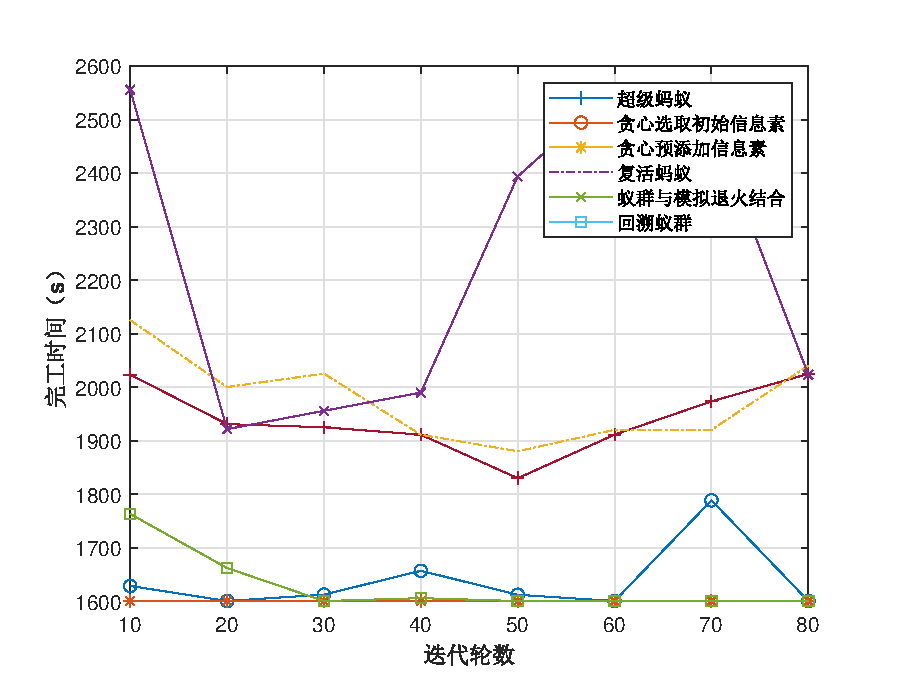
\includegraphics[scale=1.00,angle=0]{figures/test1.eps}\\
	\caption{蚁群算法各个优化思路迭代轮数与完工时间关系(10到80轮)}
\end{figure}

如上图所示,按迭代轮数与完工时间关系曲线的运动趋势可将6种优化思路分为3类:随迭代轮数增加,完工时间先递减后在较高值处振荡、完工时间始终在迪杰斯特拉解附近、随迭代轮数增加完工时间有收敛到迪杰斯特拉解的趋势。

关系曲线符合随迭代轮数增加,完工时间先递减后在较高值处振荡的优化思路有:超级蚂蚁、复活蚂蚁、蚁群与模拟退火结合

关系曲线符合完工时间始终在迪杰斯特拉解附近的优化思路有:贪心选取初始信息素、贪心预添加信息素

关系曲线符合随迭代轮数增加完工时间有收敛到迪杰斯特拉解的趋势的优化思路有:回溯蚁群

各种优化思路均对解产生了效果,单纯从解质量来看贪心选取初始信息素、贪心预添加信息素、回溯蚁群均能求解出接近迪杰斯特拉算法的解。
接下来将对各优化思路的类别进行分析。

\subsection{对随迭代轮数增加,完工时间先递减后在较高值处振荡的优化思路进行分析}
超级蚂蚁、复活蚂蚁、蚁群与模拟退火结合这三种思路随迭代轮数增加,完工时间先递减后在较高值处振荡。
将其与原始蚁群相比较,可以发现这三种优化思路都能够加快低迭代轮数时完工时间下降的速度。
复活蚂蚁机制的完工时间下降速度低于超级蚂蚁机制。
但是随着迭代轮数的继续增加,完工时间下降的趋势明显减缓,最终会在一个较高值附近振荡。
加入模拟退火机制的算法的振荡幅度显著高于其他两种机制,并且前期完工时间是从较高值快数下降的。

对于超级蚂蚁来说,如果发现更优的解,更优解会被添加上远高于其他解的信息素,前期几乎所有蚂蚁都会被引导上某条更优解。
但是基于上一节对第四章模型解分布的分析,最优解附近存在大量死锁,有走向最优解的蚂蚁很容易遇到死锁提前结束循迹。
因此即便使用超级蚂蚁,最优解上积累的信息素也会很快被其他互通的较差解超过。
算法无法收敛到最优解。

对于复活蚂蚁来说,前期完工时间下降快是因为提前结束循迹的蚂蚁被其他蚂蚁替代复活后,有效蚂蚁的数量大大增加,
实际上相当于增加了蚂蚁数量。
但是因为走向最优解并遇到死锁提前结束循迹蚂蚁会被走向较差解的蚂蚁替代,算法依然无法收敛到最优解。

对于模拟退火来说,在还未探索到较优解时,逐步提高后期蚂蚁,将避免算法局部收敛,因此算法前期波动会更大。
后期受第四章模型特殊的解分布的影响,拥有更高地位的蚂蚁反而会更剧烈地把解引导到互通的差解区域。
因此后期的解依然波动很大。

综上这三种机制并不适合求解类似第四章模型的时间Petri网。

\subsection{对完工时间始终在迪杰斯特拉解附近的优化思路进行分析}
贪心选取初始信息素、贪心预添加信息素这两种优化思路完工时间始终在迪杰斯特拉解附近。
这两种思路都和贪心的思想紧密相关。
有可能第四章模型本身适合使用贪心算法求解,因此需要排除贪心算法本身对解的影响才能分析蚁群算法效果。

使用贪心算法对第四章模型进行求解,结果如下:

变迁序列为:$t_{1}$->$t_{7}$->$t_{1}$->$t_{2}$->$t_{1}$->$t_{17}$->$t_{3}$->$t_{7}$->$t_{16}$->$t_{1}$->$t_{23}$->$t_{2}$->$t_{1}$->$t_{17}$->$t_{27}$->$t_{7}$->$t_{16}$->$t_{1}$->$t_{2}$->$t_{1}$->$t_{4}$->$t_{14}$->$t_{24}$->$t_{12}$->$t_{22}$->$t_{1}$->$t_{13}$->$t_{29}$->$t_{11}$->$t_{22}$->$t_{1}$->$t_{14}$->$t_{12}$->$t_{22}$->$t_{20}$->$t_{18}$->$t_{1}$->$t_{4}$->$t_{14}$->$t_{24}$->$t_{12}$->$t_{22}$->$t_{20}$->$t_{18}$->$t_{13}$->$t_{1}$->$t_{29}$->$t_{11}$->$t_{22}$->$t_{20}$->$t_{18}$->$t_{14}$->$t_{1}$->$t_{12}$->$t_{22}$->$t_{20}$->$t_{18}$->$t_{1}$->$t_{4}$->$t_{14}$->$t_{24}$->$t_{12}$->$t_{22}$->$t_{20}$->$t_{18}$->$t_{13}$->$t_{20}$->$t_{18}$->$t_{8}$->$t_{29}$->$t_{22}$->$t_{14}$->$t_{20}$->$t_{18}$->$t_{9}$->$t_{22}$->$t_{20}$->$t_{18}$->$t_{20}$->$t_{18}$->$t_{4}$->$t_{10}$->$t_{9}$->$t_{24}$->$t_{22}$->$t_{6}$->$t_{8}$->$t_{22}$->$t_{28}$->$t_{10}$->$t_{20}$->$t_{18}$->$t_{9}$->$t_{22}$->$t_{20}$->$t_{18}$->$t_{20}$->$t_{18}$->$t_{4}$->$t_{10}$->$t_{9}$->$t_{22}$->$t_{20}$->$t_{18}$

完工时间为:1600.8s

程序运行时间为:0.065s

变迁序列和完工时间均与迪杰斯特拉解一样,因此此网的贪心解就是最优解。

原模型为S3PR模型,本就适合最早加工策略的调度,因此使用贪心算法就能求出最优解。
破坏原模型的顺序结构,使其加工腔的晶圆可以重入得到网1 。

基于上文的分析,算法收敛到差解的主要原因是此模型存在死锁,因此需要研究算法在无死锁模型下的情况。
网1存在大量死锁,对网1进行死锁控制形成网2 。
对网1、网2使用100只蚂蚁的蚁群算法分别从10轮每次递增10轮直到80轮进行测试两种优化思路,观察完工时间。

网1的测试结果如下:

\begin{table}[H]
	\centering
	\caption{网1各优化思路完工时间与迭代轮数关系}
	\resizebox{!}{!}{
		\begin{tabular}{c|cccccccccc}
			\toprule
			\diagbox{优化思路}{完工时间(s)}{迭代轮数} & 10 & 20 & 30 & 40 & 50 & 60 & 70 & 80  \\
			\hline
			贪心选取初始信息素 & 2554.7 & 2124.5 & 2024.1 & 1973.7 & 1921.1 & 1973.7 & 1990.0 & 1973.7  \\
			贪心预添加信息素 & 2393.8 & 2024.5 & 2024.5 & 2024.1 & 1973.7 & 1920.7 & 1973.1 & 1921.1  \\
			\bottomrule
		\end{tabular}
	}
\end{table}

网2的测试结果如下:

\begin{table}[H]
	\centering
	\caption{网2各优化思路完工时间与迭代轮数关系}
	\resizebox{\linewidth}{!}{
		\begin{tabular}{c|cccccccccc}
			\toprule
			\diagbox{优化思路}{完工时间(s)}{迭代轮数} & 10 & 20 & 30 & 40 & 50 & 60 & 70 & 80  \\
			\hline
			贪心选取初始信息素 & 2040.5 & 2034.5 & 1911.5 & 1820.3 & 1788.9 & 1763.5 & 1662.4 & 1600.8  \\
			贪心预添加信息素 & 2554.7 & 2120.1 & 1973.7 & 1900.5 & 1820.3 & 1788.9 & 1700.5 & 1606.2  \\
			\bottomrule
		\end{tabular}
	}
\end{table}

\begin{figure}[H]
	\centering
	% Requires \usepackage{graphicx}
	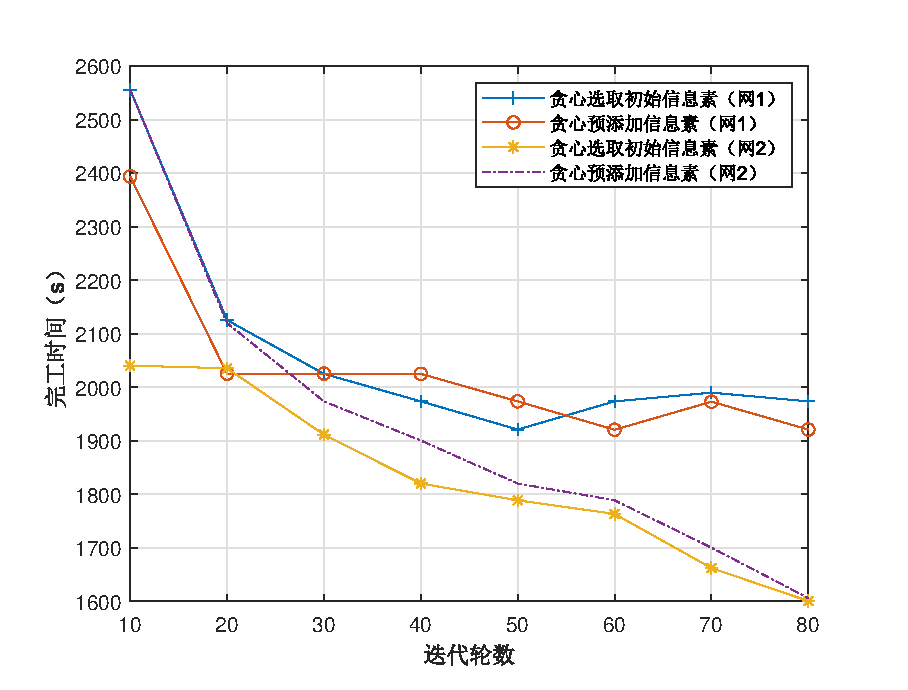
\includegraphics[scale=1.00,angle=0]{figures/test2.eps}\\
	\caption{贪心优化思路迭代轮数与完工时间关系(10到80轮)}
\end{figure}

如上图所示,如果不做死锁控制,加入贪心机制的蚁群算法依然无法收敛到最优解。
因此对于最优解附近有大量死锁的时间Petri网,这两种优化思路效果有限。但是如果在使用蚁群求解前,预先消除Petri网死锁,算法将会有很好的收敛效果。

\subsection{对随迭代轮数增加完工时间有收敛到迪杰斯特拉解的趋势的优化思路进行分析}
只有回溯蚁群机制一种优化思路能让算法随迭代轮数增加完工时间有收敛到迪杰斯特拉解的趋势。

本次测试回溯蚁群时蚂蚁寿命上限是使用统计平均寿命的方法实现的。
对静态蚂蚁寿命和最小蚂蚁寿命也在相同条件下进行实验,静态蚂蚁寿命设置为100 。

\begin{table}[H]
	\centering
	\caption{各寿命上限机制与完工时间与迭代轮数关系}
	\resizebox{!}{!}{
		\begin{tabular}{c|cccccccccc}
			\toprule
			\diagbox{蚂蚁寿命上限机制}{完工时间(s)}{迭代轮数} & 10 & 20 & 30 & 40 & 50 & 60 & 70 & 80  \\
			\hline
			静态蚂蚁寿命 & 2359.2 & 2120.1 & 1983.1 & 1900.5 & 1880.4 & 1780.5 & 1730.5 & 1616.2  \\
			最小蚂蚁寿命 & 2492.3 & 2020.4 & 2123.1 & 2124.7 & 2374.2 & 2522.5 & 2473.3 & 2554.7  \\
			\bottomrule
		\end{tabular}
	}
\end{table}

\begin{figure}[H]
	\centering
	% Requires \usepackage{graphicx}
	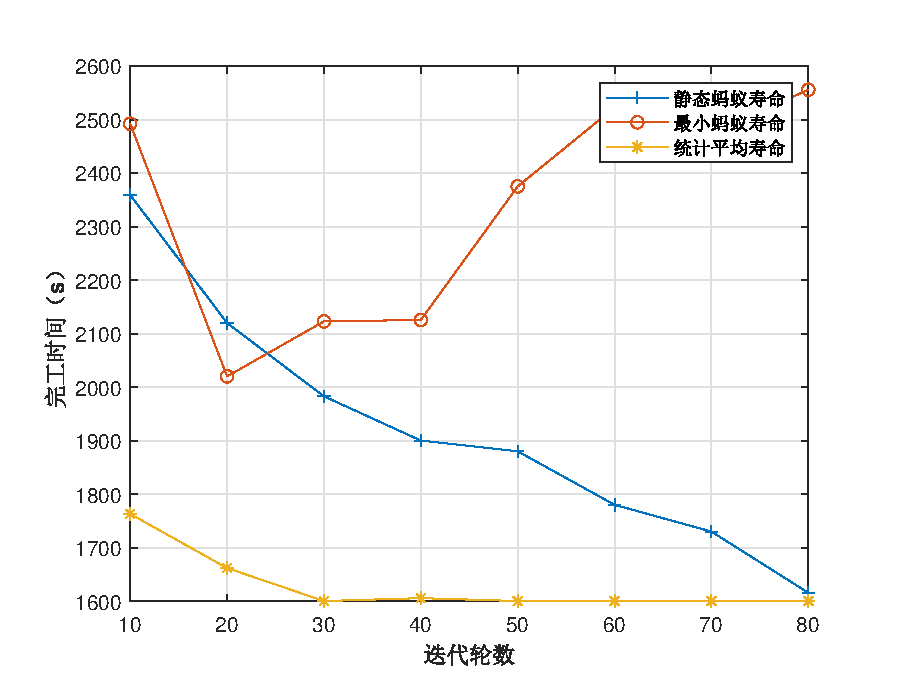
\includegraphics[scale=1.00,angle=0]{figures/test3.eps}\\
	\caption{不同蚂蚁寿命上限机制与完工时间关系(10到80轮)}
\end{figure}

如上图所示,静态蚂蚁寿命与统计平均寿命能够使算法收敛到最优解,但是最小蚂蚁寿命机制随着迭代轮数的增加,解的质量会恶化。

其原因可能是使用最小蚂蚁寿命机制时,算法后期的蚂蚁寿命上限过低,以至于蚂蚁失去回溯能力,无法走上死锁过多的路径。

统计使用最小蚂蚁寿命机制与统计平均寿命时,蚂蚁寿命上限与迭代轮数的关系。

\begin{table}[H]
	\centering
	\caption{各寿命上限机制与寿命上限与迭代轮数关系}
	\resizebox{!}{!}{
		\begin{tabular}{c|cccccccccc}
			\toprule
			\diagbox{寿命机制}{寿命上限}{迭代轮数} & 10 & 20 & 30 & 40 & 50 & 60 & 70 & 80  \\
			\hline
			静态蚂蚁寿命 & 83 & 24 & 10 & 1 & 1 & 1 & 1 & 1  \\
			统计平均寿命 & 167 & 201 & 123 & 25 & 12 & 15 & 10 & 13  \\
			\bottomrule
		\end{tabular}
	}
\end{table}

\begin{figure}[H]
	\centering
	% Requires \usepackage{graphicx}
	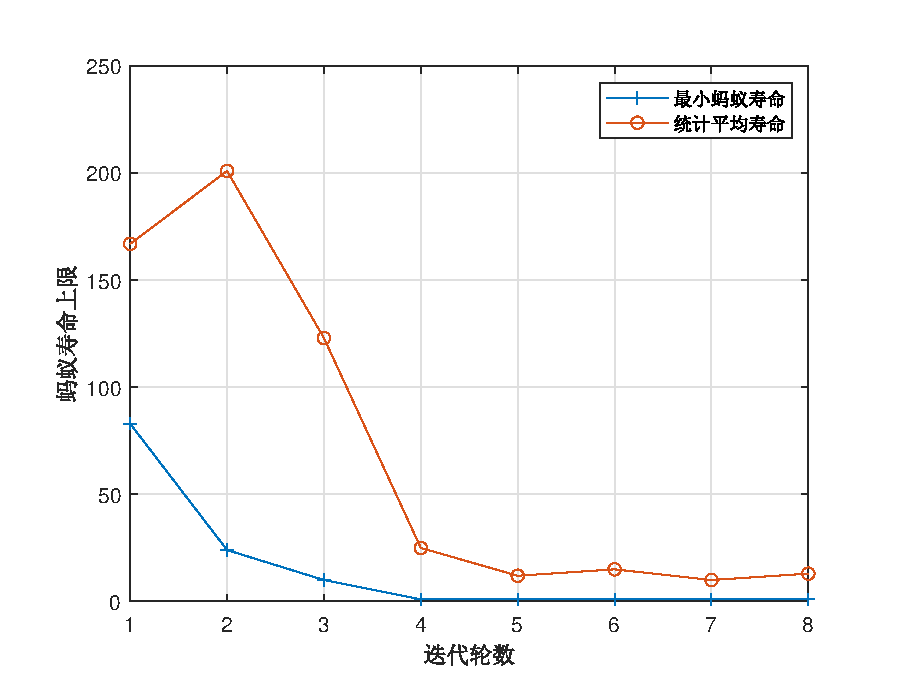
\includegraphics[scale=1.00,angle=0]{figures/test4.eps}\\
	\caption{不同蚂蚁寿命上限机制蚂蚁寿命上限与迭代轮数的关系(10到80轮)}
\end{figure}

如上图所示,使用最小蚂蚁寿命时,蚂蚁寿命上限很快降低到最小值,以至于后期蚂蚁几乎没有回溯能力。
但使用统计平均寿命时蚂蚁寿命上限最终收敛于12左右,依然具备一定的回溯能力,并且远小于直接配置静态寿命100,大大节约了程序运行时间。

\subsection{CPU数量对回溯蚁群算法速度的影响}
基于本章第1节对本蚁群算法流程的描述,本文所使用的蚁群算法为多线程算法。
所有蚂蚁均可并行地探索可达图,蚂蚁数量越多,在CPU数量不做限制时,算法将寻找到更多的解。
因此不论从解质量还是程序运行时间的角度看蚂蚁数量越多越好。

但是根据4.4.3.2节的实验数据,当蚂蚁数量在10以上时,再增加蚂蚁数量对解贡献就不大了。
而实际情况下CPU数量是有限的,线程切换时会有额外的CPU资源的开销,因此不宜设置过高的蚂蚁数量。

迪杰斯特拉算法是单线程算法,不会受到CPU数量影响,因此提升CPU数量无法减小程序运行时间。
在使用了m1 ultra的Mac Studio上使用迪杰斯特拉算法计算第四章建立的时间Petri网模型,程序运行时间为7.232s。
以此为基准,使用100只蚂蚁的蚁群算法迭代100轮,统计不同CPU数量下程序运行时间。

\begin{table}[H]
	\centering
	\caption{各寿命上限机制与寿命上限与迭代轮数关系}
	\resizebox{\linewidth}{!}{
		\begin{tabular}{c|cccccccccccc}
			\toprule
			CPU数量 & 11 & 12 & 13 & 14 & 15 & 16 & 17 & 18 & 19 & 20 \\ \hline
			程序运行时间(s) & 23.525 & 14.312 & 8.753 & 6.624 & 4.231 & 4.441 & 3.001 & 2.121 & 1.361 & 1.214 \\
			\bottomrule
		\end{tabular}
	}
\end{table}

\begin{figure}[H]
	\centering
	% Requires \usepackage{graphicx}
	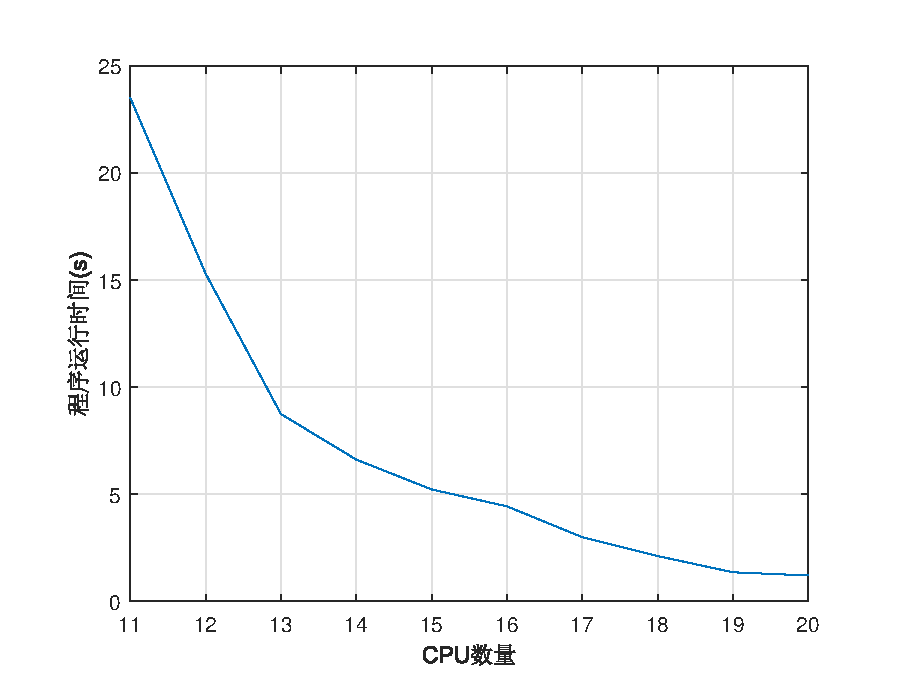
\includegraphics[scale=1.00,angle=0]{figures/test5.eps}\\
	\caption{蚁群算法不同CPU数量下程序运行时间}
\end{figure}

如上图所示,当开启14个CPU时,程序运行时间就已经优于迪杰斯特拉算法了,继续增加CPU数量能显著提升算法效果。

\section{本章小结}
本章提出了一种基于时间Petri网的蚁群算法,使用此算法求解上一章模型的调度策略,并与迪杰斯特拉算法相比较。
发现蚁群算法的解明显劣于迪杰斯特拉算法,
而且随迭代轮数增加,算法不能收敛。
于是基于实际情况,设计了6种优化方案,最终回溯蚁群策略效果明显。
% \chapter{总结与展望}
\section{总结}
晶圆制造系统是用于生产半导体芯片的设备和工艺的集合体。
它由多个工艺步骤组成,包括晶圆清洗、切割、涂覆、曝光、蚀刻、离子注入、金属沉积等。
晶圆制造系统通常由多个设备组成,包括晶圆清洗机、曝光机、蚀刻机、离子注入机、金属沉积机等。
这些设备通常由自动化系统控制,以确保工艺步骤的准确性和一致性。
本文使用Petri网对实际的晶圆制造系统进行建模,并设计蚁群算法求此系统进行调度。

本文第二章介绍了Petri网的基本理论,总结了各种调度算法。
并且梳理了一系列时间Petri网的相关知识。

第三章根据晶圆制造系统的特点,结合了第二章介绍的变迁时间网可库所时间网,提出了一种新的时间网子类,变迁库所时间网。
并且设计了一种此时间网变迁发射的时间计算流程,以保证变迁发射后系统时间尽可能短,以及一个用于计算各种Petri网模型的程序架构,供后续调度算法使用。
之后使用变迁库所时间网对一个实际的晶圆制造系统进行建模。

第四章使用蚁群算法对第三章建立的模型进行调度。
但发现调度结果不能收敛到最优解,通过对解的分析,从不同角度提出了6种优化思路,
最终回溯蚁群算法效果显著。
\section{展望}
\subsection{变迁库所时间网的进一步优化思路}
如果晶圆需要进入一系列的加工腔加工,并且规定此晶圆从进入第一个加工腔开始,必须在规定时间内完成加工,最直观的做法是有某套机制能够跟踪晶圆。
晶圆由托肯表示,各托肯在Petri网中是无法区分的。
因此之后可以设计并开发一套托肯编号机制。

实际的Petri网系统中,既有托肯表示晶圆,也有表示逻辑值,这类托肯在被变迁移动时所进入的库所是不同的,
并且实际系统中存在多个晶圆交换操作。
因此应该设计一套托肯移动的规则,以保证上述逻辑的正确。
\subsection{蚁群算法的进一步优化思路}
对于蚁群算法的进一步优化,可以从时间和空间两个方面入手。
减少算法的时间开销可以通过阻止蚂蚁探索无意义的标识实现;
减少空间开销可以设计更高效的数据结构来实现。
\subsubsection{全局时间禁忌表}
本文结合Petri网的实际情况,提出了回溯蚁群算法并取得了不错的成果。
蚂蚁能够回溯后便拥有了发现不可行解的能力。
如果将这批不可行解记录下来,下一轮蚁群循迹时提前禁止蚂蚁走上不可行解,将大大提高蚁群算法收敛速度。
不可行解由标识组成,因此可以使用一个新的集合存储这些标识。
此集合用于避免蚂蚁走上无意义的标识,功能与禁忌表相似,
因此将其命名为全局禁忌表。

而本算法是基于时间Petri网的,
此Petri网超过时间约束也会引发死锁,
此类死锁受时间因素影响不能简单的判定为不可行解。

综上全局禁忌表存储的应该为一系列的键值对,键为不可行解中的标识向量,
值应为一系列的充分条件。
如果蚂蚁探索到的标识满足这一系列的条件,则意味着继续探索不可能到达终点标识。
这一系列的充分条件会随着蚁群的探索一步步细化,逼近充要条件。
\subsubsection{实现禁忌表新的数据结构}
如果将Petri网的标识向量编码为二进制串,有一种比哈希表更高效的数据结构,二元决策图可以以更低的空间开销存储二进制信息。
蚁群算法为多线程算法,更为适合在GPU上运行,GPU的显存带宽远高于内存带宽,但通常来说显存大小不如内存,并且显存与内存通信需要消耗时间。
因此可以使用布隆过滤器在显存和内存间做一层中间层,把显存中长期未处理过的标识转移入内存中。
内存与硬盘间也可以使用相似的逻辑,这样可以极大提升存储标识的数量。
\chapter{绪论}
\section{研究背景和意义}

\section{国内外研究现状}
\chapter{相关技术概述}
\section{相关算法}
\subsection{RFM模型}
RFM分析模型\cite{hughes2005strategic}是一种基于客户行为数据的分析方法。该模型站在企业的视角,通过综合考量客户的一般购买行为,帮助企业评估和理解客户的价值。RFM模型主要依据三个关键维度来评价客户价值:近度(Recency, R)、频度(Frequency, F)和额度(Monetary, M)。

近度(Recency, R):此维度衡量的是自客户最后一次消费行为至样本采集时间点的间隔长度。这个间隔时间越短,表示客户最近对产品或服务的兴趣越高,相应地,这类客户的价值就更高。在具体的业务场景中,近度指标需要根据企业的特点和市场环境加以调整和解释。

频度(Frequency, F):该维度反映的是在特定时间段内客户消费行为的总次数。频率更高的客户表明他们与企业的交互更为频繁,通常意味着更高的客户忠诚度和更大的价值。企业需要基于历史交易数据来分析客户的消费频次,以识别出忠实用户群体,并制定策略以增强客户粘性和防止客户流失。

额度(Monetary, M):此指标是指在一个确定的时间段内客户的总消费额。一般而言,消费额度越高的客户被认为对企业更为重要,因为他们为企业带来了更多的收入。基于用户的累计消费额,企业可以识别出高价值客户,并通过制定VIP机制或者其他形式的客户回馈机制来提升这些客户的体验和满意度。

通过对近度、频度和额度三个维度的综合考量,企业能够更精准地理解和满足客户的需求,从而促进客户忠诚度的提升和企业收益的增长。
\subsection{核密度估计}
核密度估计\cite{10.1214/aoms/1177728190}(Kernel Density Estimation,简称KDE)是一种用于估算随机变量的概率密度函数的非参数方法。相对于传统的直方图估计,核密度估计能提供更为平滑的概率分布估计。该方法对于探索数据的潜在分布特征尤为重要,尤其是当我们缺乏关于数据分布先验知识时。

在核密度估计中,每个样本点都被视为一个“核”,这个核可以被理解为围绕样本点的一种平滑的概率质量分布。核函数通常选择满足一定条件的函数,如非负性、积分为一(确保整体是概率分布)等,常见的核函数有高斯核、均匀核、三角核等。

核密度估计的公式如式\eqref{eq:KDE}所示。
\begin{equation}
    f(x) = \frac{1}{n}\sum_{i=1}^{n} \frac{1}{h}K\left(\frac{x-x_i}{h}\right)
    \label{eq:KDE}
\end{equation}
其中,\(f(x)\) 是估计的密度函数,\(n\) 是样本数量,\(x_i\) 是单个样本点,\(K(\cdot)\) 是核函数,\(h\) 是带宽参数,控制核的宽度,即平滑参数。带宽的选择对核密度估计的结果影响显著:带宽过小会导致估计结果过于崎岖,呈现过多的波动,即过拟合;而带宽过大则会导致估计过于平滑,无法准确反映数据的分布特性,即欠拟合。

在实际应用中,核密度估计广泛用于数据科学和统计学中,用于数据可视化、概率分布估计、异常点检测以及作为其他统计方法的基础。在进行核密度估计时,合理选择核函数和带宽参数对于获得准确、可靠的估计结果至关重要。通过核密度估计,研究者可以更加直观地理解数据集的分布特征,为后续的数据分析和决策提供支持。

\subsection{门控循环单元}
门控循环单元(Gated Recurrent Unit, GRU)是循环神经网络(Recurrent Neural
Network, RNN)的变体。循环神经网络(RNN)是一种专门用于处理序列数据的神经网络。它的内部结构包括一个循环单元,用于存储过去的信息,使网络能够利用之前的信息来处理当前的输入。这种结构允许信息随时间传递,使得RNN特别适用于时间序列数据或任何形式的有序数据。在RNN中,每个节点都接收前一个时间步的输出和当前时间步的输入作为其输入,创建了一个在时间上循环的网络。
原始的RNN在处理长期依赖问题时表现不佳,容易出现梯度消失和梯度爆炸的问题,这使得模型难以从长序列中有效地学习信息。为了解决这个问题,研究者们提出了LSTM(长短期记忆)和GRU(门控循环单元)两种变体,通过加入门控的方式选择性地保留长期依赖。
与传统的RNN相比,LSTM的独特之处在于其内部结构,它包含有三个重要的门控机制:忘记门、输入门和输出门,以及一个持久的细胞状态,这些共同工作以保持和调节信息流。其中忘记门负责决定哪些信息应从细胞状态中移除,这通过观察当前输入和上一个时间步的隐藏状态来决定,帮助网络忘记那些不再重要的信息。
输入门决定哪些新信息将被存储在细胞状态中,使网络能够更新其存储的信息以反映新接收到的重要数据。输出门控制从细胞状态到隐藏状态的信息流,确定下一个时间步的输出应该包含哪些内容。
细胞状态则像一条传送带,横贯整个LSTM结构,只有通过门控制的微小调整,允许信息无阻碍地流过整个链。这种设计使得LSTM能够在长时间间隔内保存状态和记忆,有效避免了传统RNN中常见的梯度消失问题。
GRU是一种与LSTM相似的RNN架构,但结构上更为简化。其旨在解决传统RNN无法有效处理长期依赖问题的同时,减少计算复杂度和模型参数量,从而加快训练速度并减少计算资源需求。
GRU的关键在于它将LSTM中的三个门(忘记门、输入门和输出门)简化为两个门:更新门(Update Grate)和重置门(Reset Grate)。其中更新门决定了从一个状态到另一个状态有多少信息是需要更新的。更新门帮助模型决定在当前状态的信息中保留多少旧信息和加入多少新信息。它类似于LSTM中的忘记门和输入门的结合。
重置门用来决定在计算新状态时应该忽略多少之前的信息。通过这种方式,重置门允许模型抛弃和忘记不重要的信息,有助于捕捉数据中的短期依赖特征。
除了门控机制,GRU中还有一个重要的概念是隐藏状态(Hidden State),它类似于LSTM中的细胞状态和隐藏状态的结合体,但更加简化。隐藏状态在每个时间步被更新,并用于捕获并传递序列中的信息。
与LSTM相比,GRU的优势在于模型结构更简单,这意味着它们需要更少的参数,从而减少了内存消耗,加快了训练速度。LSTM和GRU的结构如图\ref{fig:lstmandgru}所示。
\begin{figure}[H]
    \centering
    \caption{LSTM/GRU结构示意图}
    \label{fig:lstmandgru}
\end{figure}
\subsection{Transformer模型}
在神经网络发展过程中,面对计算性能的限制和模型复杂度的增加,信息过载成为了一个突出问题。为应对这一挑战,业界借鉴人脑处理信息的策略,提出了注意力机制(Attention)。这一机制通过集中关注对当前任务更为关键的信息,同时忽略不相关的数据,从而提高神经网络的处理效率和性能。

注意力机制的核心原理是对信息进行加权处理,增加关键信息的重量,减少无关信息的影响。这一机制通过三种向量实现:查询向量$\mathbf{Q}$(Query)、关键向量$\mathbf{K}$(Key)和值向量$\mathbf{V}$(Value)。其中,查询向量代表与当前任务相关的需求,关键向量代表数据的关键属性,两者相互作用生成一个注意力分布,进而决定值向量中哪些信息是当前步骤需要关注的。

Transformer模型是一种完全基于注意力机制的架构,由Google公司开发\cite{vaswani2023attention}。它能够进行并行计算,有效捕捉长距离的依赖关系。该模型采用了编码器-解码器(Encoder-Decoder)结构,整个流程包括数据输入、编码处理、解码处理和最终输出四个主要部分,能够处理各种序列到序列的任务。

(1)数据输入

序列数据首先通过输入嵌入(Input Embedding)转换为嵌入向量,以此表示数据中的每个元素。随后,为了让模型能够识别序列中每个元素的位置,会为每个嵌入向量增加位置编码PE(Positional Encoding)。这样可以保持序列的顺序信息。
PE的计算过程如公式\eqref{pos2i}和公式\eqref{posi}所示。
\begin{equation}
    PE(pos, 2i) = \sin\left(\frac{pos}{10000^{2i/d_{\text{model}}}}\right)
    \label{pos2i}
\end{equation}
\begin{equation}
    PE(pos, 2i+1) = \cos\left(\frac{pos}{10000^{2i/d_{\text{model}}}}\right)
    \label{posi}
\end{equation}
式中,\textit{pos} 代表序列中某一数据点在整个序列中的绝对位置,\(d_{\text{model}}\) 代表数据的嵌入向量维度,而 \textit{i} 表示向量中的具体维度位置。此外,\(2i\) 和 \(2i + 1\) 分别代表向量中的偶数和奇数位置维度。这种表示方法有助于在位置编码过程中区分不同位置的数据点。

(2)Encoder

在Transformer模型的编码器中,已处理的输入数据以向量形式通过多头注意力机制,随后结合残差连接和层归一化操作(统称为Add\&Norm),以及通过前馈神经网络进行进一步处理。这一系列步骤旨在增强模型对不同输入数据间关系的理解,并提高模型的学习能力及其对序列数据的处理效率。
其中注意力机制的计算过程如公式\eqref{tranatten}所示。
\begin{equation}
    \text{Attention}(Q,K,V) = \text{softmax}\left(\frac{QK^T}{\sqrt{d_k}}\right)V
    \label{tranatten}
\end{equation}
在该文中,\(\mathbf{Q}\)、\(\mathbf{K}\)和\(\mathbf{V}\)分别是输入数据\(\mathbf{X}\)与相应的权重矩阵\(\mathbf{W^Q}\)、\(\mathbf{W^K}\)和\(\mathbf{W^V}\)相乘后得到的向量。这里,\(d_k\)表示向量\(\mathbf{K}\)的维度。softmax归一化指数函数被应用于这些向量的乘积,以将它们映射到一个概率分布上,其值位于区间[0,1]之内,并且所有数值的和为1。
多头自注意力层(MHSA)通过将查询、键和值向量分割成h个较小的子向量组,每组进行独立的自注意力计算,然后将这些结果拼接起来。这种方法不仅减少了计算量,还允许模型在不同的表示子空间中捕捉信息,增强了模型理解全局特征互相关性的能力。
其表达式如式\eqref{trasmuti}所示。
\begin{equation}
    \begin{aligned}
        \text{MultiHead}(Q, K, V) = \text{Concat}(head_1, \ldots, head_h)W^Q \\
        \text{where } head_i = \text{Attention}(QW_i^Q, KW_i^K, VW_i^V)
        \label{trasmuti}
    \end{aligned}
\end{equation}
通过使用一组不同的权重矩阵\(W^Q\)、\(W^K\)和\(W^V\)来生成多组查询向量\(\mathbf{Q}\)、键向量\(\mathbf{K}\)和值向量\(\mathbf{V}\)。每一组的这些向量相互作用,分别产生一个输出矩阵\(\mathbf{Z}\)。最终,这些输出矩阵\(\mathbf{Z}\)被拼接成一个更大的矩阵,以获得综合的信息表达。   
Add\&Norm操作包括两个步骤:首先是残差连接,它将多头注意力的输出\(\mathbf{Z}\)矩阵与输入\(\mathbf{X}\)矩阵相加;其次是归一化,使用层归一化(Layer Normalization)技术对加和后的结果进行标准化,确保数据在一个合理的范围内。
前馈神经网络的计算过程如式\eqref{ffn}所示。
\begin{equation}
    \text{FFN}(x) = \max(0, xW_1 + b_1)W_2 + b_2
    \label{ffn}
\end{equation}
x代表从多头注意力机制得到的输出\(\mathbf{Z}\)矩阵。这个矩阵首先通过一个线性变换过程,然后应用ReLU激活函数进行非线性转换,筛选重要的信号。最后,这个过程通过另一个线性变换完成,产生最终的输出。

(3)Decoder 

Decoder和Encoder的计算原理基本相同,但Decoder增加了掩码多头注意力机制,这一机制通过引入掩码(mask)来修改多头注意力计算过程。其中,padding mask用于处理不同长度的序列,保证数据对齐,而sequence mask防止Decoder提前看到未来的信息,确保每个位置只能依赖于它之前的位置,从而保护序列数据的时序完整性。

(4)输出

从Decoder接收的输入数据首先经历一次线性变换,然后通过softmax函数进行处理,最终输出预测结果。

\section{数据存储}
\subsection{数据湖架构与 Apache Hudi}
为了克服数据管理领域中存在的特定缺陷,Dixon 引入了“数据湖”这一概念。此概念应对了传统数据仓库存在的两大核心问题:首先,现行的元数据管理方案缺乏统一性,导致数据孤岛现象,妨碍了数据集之间的互通;其次,对原始数据缺乏适当存储,结果是重要的初始数据经常被遗失。数据湖理念的提出,旨在通过提供一个集中式、灵活的数据存储解决方案,解决上述问题。

随后,数据湖的架构随着云计算技术的快速发展而演进。特别是在2015年,各大企业开始利用云存储的大规模、高可用性和低成本优势,逐步替代传统的HDFS存储方案。这一新型架构支持不同格式的数据存储,并采用分离计算与存储的架构,使其能够与多种计算引擎协同工作。

进入2019年,Hudi 数据格式的推出进一步推动了数据湖技术的发展。Hudi 提供了一种特殊的存储格式,并引入了一种增量处理框架,它可以与 Apache Spark 等计算平台协同工作,并支持ACID事务以及增量更新,使得数据的更新和写入更加高效。

Hudi 的架构包括三个主要组件:索引(通过索引机制优化写入和更新速度,维护文件ID与Hoodie键的映射关系)、数据文件(存放实际数据)以及时序元数据(相似于数据库的事务日志)。Hudi 支持两种类型的数据表:写时复制(COW)表和读时合并(MOR)表。COW表优化了读取操作,适合读取密集型应用;而MOR表优化了写入操作,适合写入密集型应用。

在数据查询方面,Hudi 支持快照查询、增量查询和读取优化查询。这些查询类型为用户提供了灵活的数据访问方法,允许他们根据需要选择最合适的查询模式。尽管MOR表在进行快照查询时可能会有延迟,但它们为写入密集的应用场景提供了优化方案。
\subsection{ClickHouse}
ClickHouse 是一种专为列式存储而设计的数据库管理系统,特别适用于实时分析场景。最初,它被应用于网络分析服务,后来转为开源项目。它的特点包括不存储元数据和最小化非必要数据,从而最大化数据处理的吞吐量,这使得ClickHouse非常适合于OLAP(在线分析处理)应用场景。

与传统的行式数据库相比,在列式存储数据库中数据是按列序列化存储的,这样在查询或处理跨多行的大量数据时更加高效,因为它只针对相关的数据列进行搜索和处理。而行式存储的数据库在添加数据时必须逐一定义每行的全部属性,导致在选择单行的多列时效率较高,但在大量数据处理方面则显得不足。

ClickHouse 的架构主要基于“列”和“字段”的概念。在这种基于列的存储结构中,一组数据被封装在一个“列”对象中,而“字段”则表示列中的某个特定值。在ClickHouse中,数据操作通常以列为单位进行,当需要处理特定的值时,则需使用“字段”对象。此外,“数据类型”用于执行来自“列”或“字段”的数据的序列化操作。而“数据块”是ClickHouse中进行数据操作的基本单位,包含上述三种对象。

在功能方面,ClickHouse 区分了“普通函数”和“聚合函数”。普通函数,通过 IFunction 接口实现,提供了许多实用函数,并以数据块为单位进行操作,而不是单独处理每行数据。与此相反,聚合函数则由 IAggregateFunction 接口定义,它们是有状态的,并且它们的状态可以进行序列化,因此能够在分布式节点之间进行增量计算。

在数据表设计中,ClickHouse 没有使用“表”对象,而是采用 IStorage 接口来代表数据表,该接口定义了数据定义、读取和写入的方法。这允许 IStorage 根据查询语句的抽象语法树需求,返回查询列的原始数据。

ClickHouse 服务器为多种客户端交互提供了接口,包括用于前后端交互的 HTTP 接口、用于本地客户端交互和执行分布式查询的 TCP 接口,以及用于复制传输信息的接口。服务器的作用是接收客户端提交的 SQL 语句并进行数据查询处理。其中,Parser 负责创建抽象语法树,Intercepter 负责解释抽象语法树,结合 IStorage 可以完成整个数据查询过程。因此,整个数据查询流程是在数据块上进行的,首先通过解析器将查询语句解析成抽象语法树,然后通过解释器对生成的抽象语法树进行解析,并创建查询通道。最终,IStorage 根据抽象语法树的指导返回查询列的数据。
\chapter{结合RFM与核密度估计的气井分类算法}
在气井开采初期,气井一经投入使用就会打破气藏的静态平衡,诸如产量、压力和产物性质等关键参数便会随之变动。随着开采活动的进行,气水关系会愈加错综复杂。产水量将持续攀升,
低压井和产水井的数量不断增长,不同气井之间的差异会日益增大。这些因素会进一步增加气井的生产管理难度。为提高管理效能,企业需利用历史产量数据对气井进行有效分类。将
表现出相似生产特性的气井进行归类和分析,以帮助揭示它们的共同生产模式。使得企业能够迅速评估气井的生产状况,掌握关键生产特征,进而及时规划出针对性强的管理策略和治
理行动,以确保气井的顺畅运作。本章使用了结合RFM与核密度估计的气井分类算法,根据根据气井的数据特征,对气井进行分类。首先对企业提供的报表数据进行整理和清洗,去除掉
报表中的冗余数据并将需要的信息批量提取出来。在获取了相应的气井信息后,使用结合RFM与核密度估计的气井分类算法来对气井进行分类,并在第四章通过实验验证经过分类后再对气井
进行预测效果会更好。
\section{问题分析}
企业气田的地质条件十分复杂,是典型的“低渗透、低压力、低丰度”气田。其单井产量小、压降速率快,随着气田不断进行规模开发,单井井数逐年增加,集气站也在不断的增大。
随着开采活动的不断进行,间歇井(气井按照固定的开关制度进行生产的气井)数量的也在逐步递增。气井在开采过程中,产量会随着井底污染、地层压力、地层渗透率、地层有效厚度
等的变化。不同气井之间的特征差异较大,需要通过合理的方式对气井进行分类。本文中初步想法是根据企业所提供报表数据,使用普通聚类算法如KMeans或者时间序列聚类算法如K-Shpae等对气井进行无监督分类。然而使用
这类聚类算法后发现该方法不具有稳定性,每次分类结果都不尽相同,无法达到向企业交付的标准。同时,对数据分布进行可视化展示以后,发现数据不是成团分布
,数据之间差异不大,不能简单地使用普通聚类算法。而采用K-Shpae进行时间序列聚类之后,发现不同类别之间无法提取出比较相似的特征,同一类别较为凌乱,
不能作为企业对气井分类的标准。经过分析发现普通的时间序列聚类算法大多是对过去时间序列的形状进行聚类,通过对K-Shape实验的数据结果\cite{Kshapeexperiment}
分析可以发现,其对于具有相似形状或模式的时间序列会有更好的分类效果,例如心跳、交通等具有相似周期性、趋势或季节性模式的时间序列。本文气井的时间序列没有
明显规律,因此其聚类效果较差。经过探索并依赖企业专家的领域知识,本文启发式的采用基于RFM\cite{birant2011data}评价参数结合核密度估计的方式来对气井进行分类。RFM模型是一种用于分析
客户价值和客户创收能力的方法,常用于数据库营销和直接营销中。将RFM模型应用于气井分类,可以充分挖掘气井的潜在价值。通过RFM模型来选取相应的参数,再根据数据的密度特征
选取相应的阈值,通过特征二值化的方法来对气井进行分类。
\section{问题描述}
在气井分类的问题的目标是将具有相似特征的气井分为一组,以帮助企业根据气井的特征更好地进行管理。此研究问题是提供某一气井相关数据,
确定其所属类别。问题的输入是气井的相关信息,单个数据可以表示为$x_i = \{x_{i1}, x_{i2}, \ldots, x_{iN}\}$,N表示特征数,输入数据集
$\mathbf{X} = \{X_{1}, X_{2}, \ldots, X_{m}\}$,m表示数据量的大小,输出是气井类别,将气井输出集表示为$\mathbf{Y}$,问题可以形式化为
求$\mathbf{X}$到$\mathbf{Y}$的一个映射$f$:$X \rightarrow Y$。
\section{算法框架}
\subsection{算法流程}\
\label{sec:K-Shapeprocess}
根据前文所述,传统的聚类方法以及基于时间的聚类方法在气井分类问题中效果较差,需要探寻一种合适的分类方法来对气井进行科学的分类。这其中的难点主要是
如何选取合适的分类模型以及合适的特征来对气井进行分类。本文采用在营销分析时常用的数据挖掘工具RFM模型来评估气井的价值。具体流程如图\ref{fig:wellcla}所示。
\begin{figure}
    \centering
    % Requires \usepackage{graphicx}
    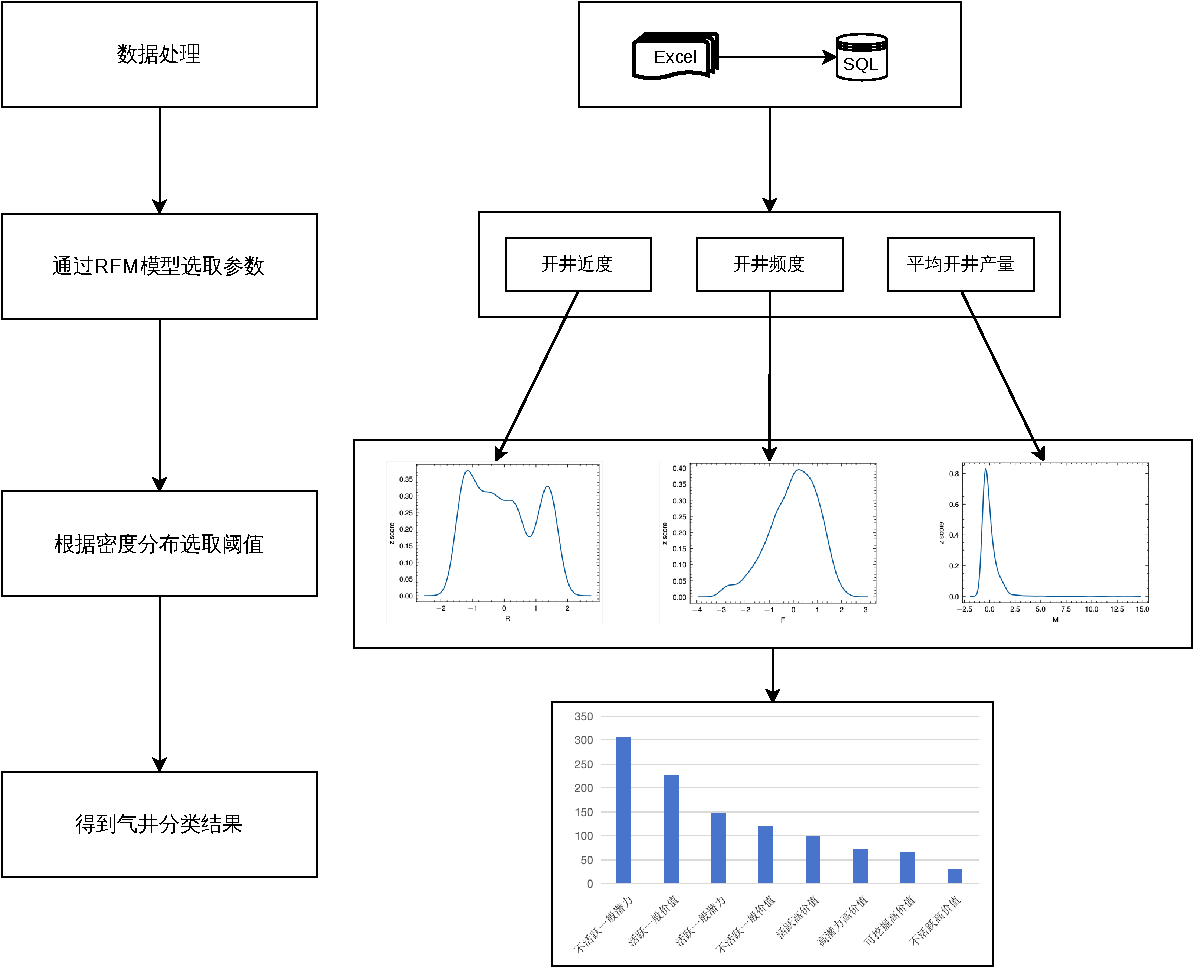
\includegraphics[width=.8\linewidth]{figure/气井分类框架图.pdf}
    \caption{结合RFM与核密度估计的气井分类算法框架图}
    \label{fig:wellcla}
\end{figure}
在进行气井数据分析的初始阶段,难题在于如何从原始报表中提取准确信息,该报表数据错综复杂且杂乱无章。为了将这些数据转化为一份规范化的报表,首先需要对原始数据进行细致的清理和整理工作。这一过程不仅涉及去除无关或重复的数据,还包括标准化数据格式和校正数据不一致性,以确保最终报表的数据质量和可靠性。

在构建规范化的数据框架之后,本文进一步利用RFM(Recency, Frequency, Monetary)模型作为分析工具来评估气井的生产性能特征。在本研究场景中,RFM模型的参数需要根据气井的生产数据特性进行相应的调整和定义。这些参数的选取和优化对于后续分析的准确性和实用性至关重要。

紧接着,本文需要对选定的参数进行密度分布分析,以根据其分布来选取合理的划分阈值。通过核密度估计(KDE)方法,可以对气井参数的分布情况进行可视化解读,从而识别出关键的数据特征和潜在的生产趋势。

最终本文利用得到的密度分布信息进行特征二值化处理。通过这种方法,本文可以有效地将气井划分为四类,为进一步的分析和决策提供支持。通过这一系列系统的数据处理和分析步骤,能够深入理解并分类气井的生产效率,为后续的资源分配和优化策略提供坚实的数据基础。
\subsection{数据处理}
\label{cha:data}
原始数据集由单井日报文件组成,涵盖了从2012年8月3日至2022年8月15日的时间跨度。这些数据以Excel格式存储,其中一个月的数据被归纳于一张多工作表的Excel文件中,一年由12张此类文件构成。每张多工作表文件包括了该月内每天的数据,每天的数据记录在单独的Excel工作表中。

每张工作表中的信息包括所属井丛、井号、配产、生产时间(包括日累和月累,月累数据自2014年4月起引入)、油压、套压(自2016年9月起引入)、井口温度、注醇量(以井丛计)、产气量(包括日产、月累、年累及历年年累)、投产日期及备注(包括开关井信息等)。

在进行数据的批量读取和处理前,需要对这些报表按照不同的格式进行分类,考虑的因素包括不同的表头、报表的组织形式、日期记录的格式,以及剔除一些非必要的表格,例如某些含有总结性信息的表格,这些信息可能会干扰批量处理。以2012年的数据为例,其格式相对杂乱,8月和9月的
数据以单独的Excel文件记录每一口井的日报,而10月至12月的数据则分别存储在三个不同的Excel文件中,每个文件包含相应月份的数据。
如表\ref{tab:examplewell}展示了气井包含信息示例。
% \begin{table}[H]
%     \renewcommand{\arraystretch}{1.5}
%     \centering
%     \caption{气井信息示例表}
%     \label{tab:examplewell}
%     \begin{tabularx}{\textwidth}{|l|Y|Y|Y|Y|}
%         \hline
%         名称 & 序号 & 丛式井 & 井号 & 配产($10^4 m^3/d$) \\
%         \hline
%         样例 & 1 & 013井丛 & AA26EF-01 & 2.3 \\
%         \hline
%         \multirow{2}{*}{名称} & \multicolumn{2}{c|}{生产时间(h)} & \multirow{2}{*}{井口压力 ($MPa$)} & \multirow{2}{*}{井口套压 ($MPa$)} \\
%         \cline{2-3} & 日产时间 & 月累 & & \\
%         \hline
%         样例 & 16.00 & 600.00 & 1.73 & 4.09 \\
%         \hline
%         \multirow{2}{*}{名称} & \multirow{2}{*}{井口温度($^\circ$C)} & \multicolumn{3}{c|}{注醇量(L)} \\
%         \cline{3-5} & & 日注醇 & 月累 & 年累 \\
%         \hline
%         样例 & 12.20 & 720 & 18000 & 39700 \\
%         \hline
%         \multirow{2}{*}{名称} & \multicolumn{4}{c|}{产气量($10^4 m^3$)} \\
%         \cline{2-5} & 日产 & 月累 & 年累 & 历年年累 \\
%         \hline
%         样例 & 1.0754 & 31.2484 & 104.4155 & 2253.7500 \\
%         \hline
%         名称 & 投产日期 & 生产方式 & 备注 & 井口油压 ($MPa$) \\
%         \hline
%         样例 & 2020/11/16 & VS & 低压\_调峰井 & 3.44 \\
%         \hline
%     \end{tabularx}
% \end{table}

\begin{table}[H]
    \centering
    \caption{气井信息示例表}
    \label{tab:examplewell}
    \begin{tblr}{
        width = \textwidth,
        colspec = {|X[l]|X[c]|X[c]|X[c]|X[c]|},
        hlines, vlines,
        columns = {valign=m},
        rows    = {halign=c, font=\renewcommand{\arraystretch}{1.5}},
        cell{3}{1} = {r=2}{c},
        cell{3}{2} = {c=2}{},
        cell{6}{1} = {r=2}{c},
        cell{6}{2} = {r=2}{c},
        cell{6}{3} = {c=3}{},
        cell{9}{2} = {c=4}{},
        cell{9}{1} = {r=2}{c},
    }
        名称 & 序号 & 丛式井 & 井号 & 配产($10^4 m^3/d$) \\
        样例 & 1 & 013井丛 & AA26EF-01 & 2.3 \\
        名称 & 生产时间(h) & & 井口压力 ($MPa$) & 井口套压 ($MPa$) \\
        & 日产时间 & 月累 & & \\
        样例 & 16.00 & 600.00 & 1.73 & 4.09 \\
        名称 & 井口温度($^\circ$C) & 注醇量(L) & & \\
        & & 日注醇 & 月累 & 年累 \\
        样例 & 12.20 & 720 & 18000 & 39700 \\
        名称 & 产气量($10^4 m^3$) & & & \\
        & 日产 & 月累 & 年累 & 历年年累 \\
        样例 & 1.0754 & 31.2484 & 104.4155 & 2253.7500 \\
        名称 & 投产日期 & 生产方式 & 备注 & 井口油压 ($MPa$) \\
        样例 & 2020/11/16 & VS & 低压\_调峰井 & 3.44 \\
    \end{tblr}
\end{table}


经过与企业专家沟通,本文选取了日期、集气站号、井序号、日产时间、井口压力(油压)、套压、井口温度、日产量和投产时间等关键指标。其中套压数据的记录是从2016年9月开始的,这个时间点之前的数据中不包括套压信息。

在批量处理和读取原始数据的过程中,首先要去除每张Excel表中的冗余信息,这包括无关的汇总信息、非结构化的备注或者其他非目标数据列。随后,从每张表中提取出所需的关键列,这一步骤将会生成每个单井每日的数据记录,每天的记录将被整理并存储在一个单独的CSV格式文
件中。处理完整个时间范围后,生成了3664个此类文件,每个文件代表一个日报的数据集,覆盖从2012年8月3日至2022年8月15日的时间段。

接下来,将这些单日数据集进行统一处理以建立一个完整的数据集,该过程包括填充空值、进行数据格式转换,并确保所有数据均以CSV格式表示。数据覆盖从2012年8月3日至2022年8月15日的时间范围。

数据合并后,接着进行数据清洗工作。这包括挑选关键列、重新命名列以确保一致性,并按时间顺序排列数据。接下来是数据类型统一化工作,包括将所有日期格式统一转换为标准格式,如“2022-08-15”,并进一步转化为标准的时间戳格式;同时,将所有数字类型统一为浮点数格式。
此外,还需处理数据中的异常值,例如,存在一些记录显示日产量极低(如0.0008),而日产时间却记录为24小时,这类数据显然不合理,因此需对这些记录进行修正。最后,对数据集中的重复值进行检查并去除,以确保数据集的准确性和完整性。最终将得到的结果保存在数据库中。

本文在进行智能分析时,从所有油井中剔除了那些生产日期小于60天的井,确保了分析的数据质量和可靠性。然后,对剩余井的历年累积产量、平均产量和峰值产量进行了统计分析。分析的统计项包括了计数(即数据的数量)、平均值、标准差(反映数据的离散程度)、
最小值、25\%分位数(第一四分位数,表示所有数据中有25\%的数据小于此值)、中位数(数据的中间值)、75\%分位数(第三四分位数,表示所有数据中有75\%的数据小于此值)以及最大值。整个分析覆盖了共910项数据,为研究人员提供了全面的统计信息,帮助他们理解油
井的生产性能和历史产量情况。具体如表\ref{tab:productionData}所示。
\begin{table}[H]
    \renewcommand{\arraystretch}{1.5} % Increase row height
    \centering
    \caption{产量统计数据表}
    \label{tab:productionData}
    \resizebox{\textwidth}{!}{
        \begin{tabular}{lrrr}
            \hline
            & \multicolumn{1}{c}{总年产量 (TotalYearly)} & \multicolumn{1}{c}{平均产量 (Average production)} & \multicolumn{1}{c}{最大产量 (Maximum production)} \\ \hline
            计数 (count) & 910 & 910 & 910 \\
            均值 (mean) & 2255.58798 & 1.409243 & 7.631090 \\
            标准差 (std) & 2304.31763 & 1.241984 & 3.793141 \\
            最小值 (min) & 1.02960 & 0.00000 & 0.00000 \\
            25\% & 796.81390 & 0.514347 & 4.905600 \\
            50\% & 1604.74685 & 1.043528 & 6.910450 \\
            75\% & 3013.33105 & 1.924211 & 9.149850 \\
            最大值 (max) & 17910.26970 & 8.884964 & 23.493800 \\ \hline
        \end{tabular}
    }
\end{table}

为了便于分析和对比各气井的产量变化趋势及其随时间的动态变化,以及观察不同气井之间的时间序列曲线是否存在交叉点,本文计划制作一套交互式折线图。这些折线图将详细展示所有井的产气量随时间变化的趋势。

在这套交互式图表中,用户将有能力选择特定的井来查看其产量变化,这使得用户能够专注于分析特定井的性能,同时也可以轻松切换查看其他井的产量数据。此外,这种交互式设计还允许用户检查曲线上每个点的具体值,从而获得详细的日产量信息。

通过这种交互式的数据可视化方法,用户不仅可以直观地观察每口气井随时间的产量变化,还可以有效比较不同井之间的产量差异,以及识别任何可能的异常或显著的趋势变化。这种分析工具将大大增强数据的可访问性和可理解性,为气井的管理和优化提供有价值的洞察。

\begin{figure}[H]
    \centering
    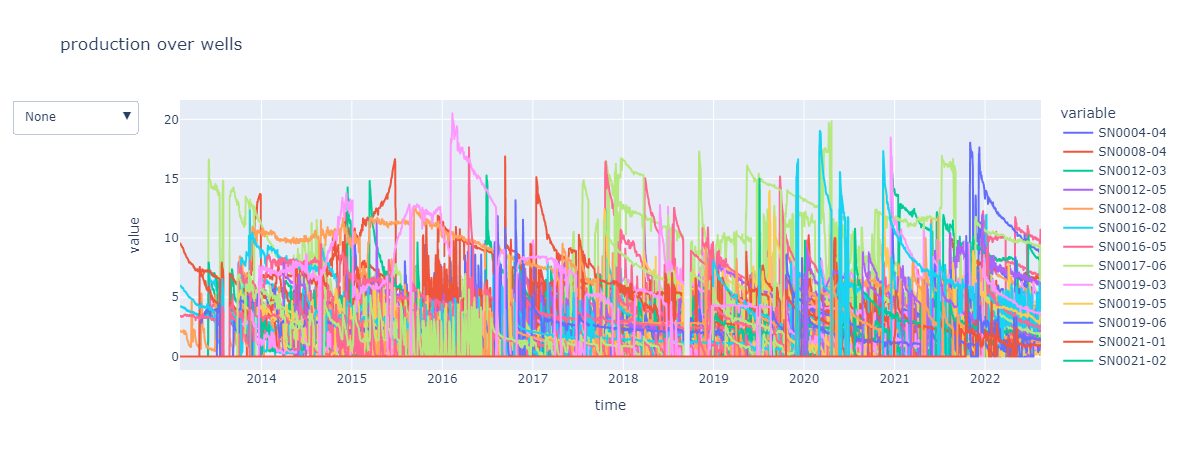
\includegraphics[scale=0.3,angle=0]{figure/productiongraph.png}
    \caption{在一张图上同时绘制多口井产量随时间的变化曲线}
    \label{fig:productionchange}
\end{figure}
\begin{figure}[H]
    \centering
    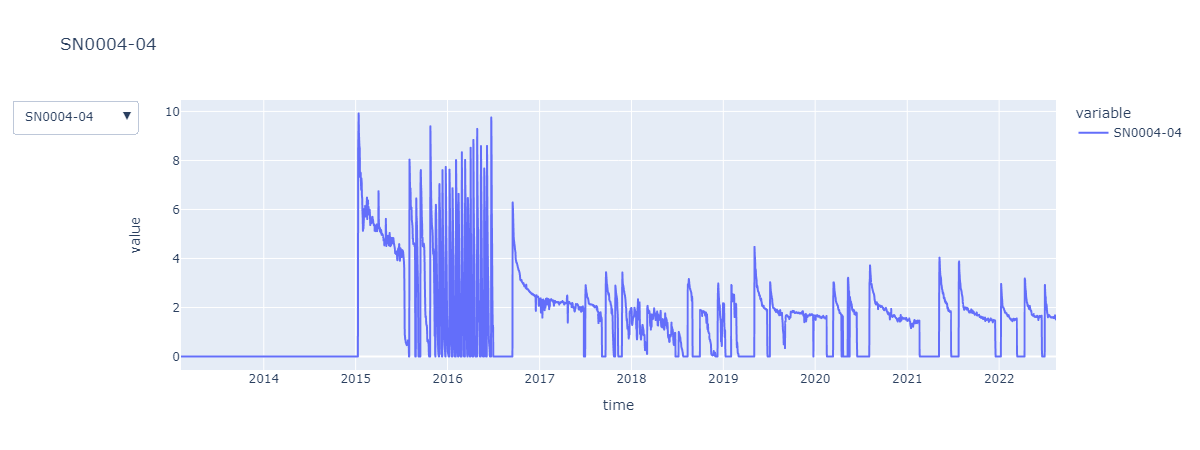
\includegraphics[scale=0.3,angle=0]{figure/awellgraph.png}
    \caption{井SN0004-04的产量随时间的变化曲线}
\end{figure}
\subsection{RFM参数选取}
RFM模型对应的各组件为最近一次购买或交互(Recency)、购买或交互的频率(Frequency)、购买的货币价值(Monetary),是一种常用于客户价值分析的方法。
尽管它最初是为零售业和直接营销设计的,用于评估客户的购买行为,但其核心概念可以被扩展和应用于各种不同领域,包括能源产业等。在气井的背景
下,RFM模型可以被重新解释和调整,以评估气井的生产特性,具体如下:

Recency (R):最小开井近度。此指标反映了自气井上一次开井以来的时间跨度。在气井的运营过程中,最小开井近度作为衡量气井活跃度和响应速度的关键
指标。其公式如\eqref{eq:R}所示。
\begin{equation}
    R_i = t_{laset} - t_{i\_last}
    \label{eq:R}
\end{equation}
式中$t_{laset}$为用户定义的最后的截止日期,$t_{i\_last}$为气井最近一次的开井时间。i表示第i个气井。

Frequency (F):开井频度。该维度代表在特定时期内气井开井的频次。其公式如\eqref{eq:F}所示。
\begin{equation}
    F_i=\frac{N_{i\_days\_opend}}{N_{days\_sampled}}
    \label{eq:F}
\end{equation}
在这个公式中,如果备注中包含“open”一词,我们就计为1,否则计为0,然后将所有的1加起来,计算的到开井的日期。最后用开井日期除以样本总日期得到
最终的开井频度。

Monetary (M):平均开井产量。在传统RFM模型中代表消费金额,在气井场景中,这可以被理解为气井的生产量或产值,高产值的气井可能更具商业价值。其公式如
\eqref{eq:M}所示。
\begin{equation}
    M_i = \frac{mean(P_i)}{N_{i\_days\_opend}}
    \label{eq:M}
\end{equation}
其计算方式是将每个井i所有的日产气加起来,得到总的产气量$P_i$,然后除以开井时间。

通过综合考虑最小开井近度、开井时间和平均开井产量这三个维度,本文采用RFM模型对气井进行分类,旨在识别不同性能和潜力的气井群体。该方法不仅为气
井的综合评估提供了一种新的视角,而且通过量化分析支持了更为精准和个性化的气井管理策略的制定。此外,RFM模型的应用促进了对气井生产特性的深入理
解,为实现资源优化配置、提升生产效率以及最大化经济回报提供了坚实的分析基础。
\subsection{核密度估计}
使用RFM模型,并选定了合适的参数进行评估后。接下来需要通过基于核密度估计(KDE)方法来确定用于分类的阈值。核密度估计是一种估计概率密度函数的非参数方式,它可以从给定数据集出发,找到其概率分布的平滑估计。

本文选取的核函数为高斯核函数,具体如式\eqref{eq:gauss}所示。
\begin{equation}
    K(u) = \frac{1}{\sqrt{2\pi}} \exp\left(-\frac{1}{2} u^2\right)
    \label{eq:gauss}
\end{equation}
采用基于Silverman的规则(Silverman's rule of thumb)来计算带宽。具体公式如式\eqref{eq:silverman}所示。
\begin{equation}
    h = \left(\frac{4\hat{\sigma}^5}{3n}\right)^{\frac{1}{5}} \approx 1.06 \hat{\sigma} n^{-1/5}
    \label{eq:silverman}
\end{equation}
这里,\( n \) 表示样本大小,而 \( \hat{\sigma} \) 是样本的标准偏差。该公式为高斯核密度估计中带宽的选择提供了经验方法。

在确定了合适的核函数和带宽后,本文通过核密度估计,获得了一个连续的密度函数。得到的核密度函数归一化后如图\ref{fig:KDE}所示。
\begin{figure}[H]
    \centering
    \subfloat[开井近度]{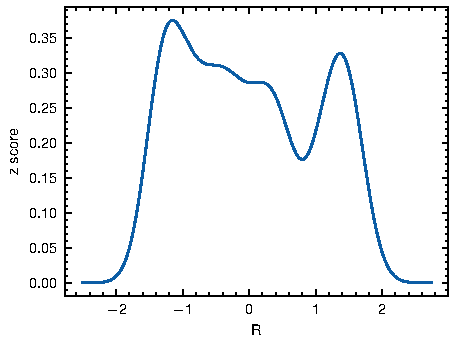
\includegraphics[width=.3\linewidth]{figure/R_z_kde.pdf}%
    \label{R}}
    \hfil
    \subfloat[开井频度]{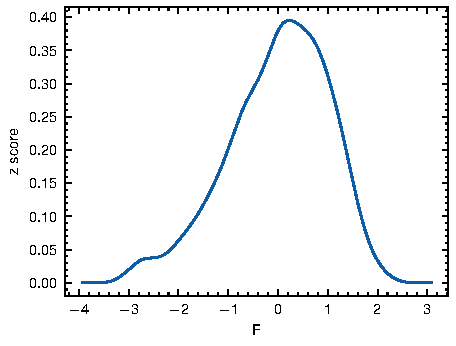
\includegraphics[width=.3\linewidth]{figure/F_z_kde.pdf}%
    \label{F}}
    \hfil
    \subfloat[平均开井产量]{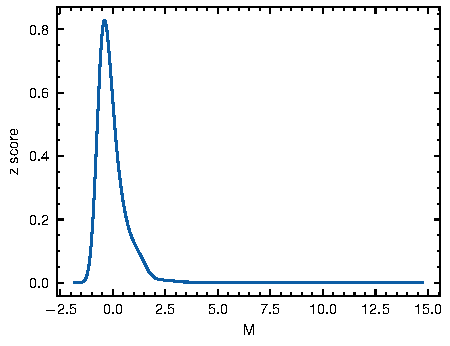
\includegraphics[width=.3\linewidth]{figure/M_z_kde.pdf}%
    \label{M}}
    \caption{核密度函数结果}
    \label{fig:KDE}
\end{figure}
\par
对于开井近度(R),由于其核密度估计结果呈现出两个明显的波峰,可以合理推断出有两种不同的工作状态。由于波谷处的开井近度较少见,可以作为两种不同工作模式的分界点,本文选取了两个波峰之间的波谷作为分类的阈值。位于左侧波峰的井被认为是近期频繁开井的,即开井
近度高;而位于右侧波峰的井则被视为近期较少开井,即开井近度低。这种分类有助于我们根据近期开井活动的频繁程度进行分析和管理。

开井频度(F)的分布呈现出接近正态分布的形态,表明大多数气井的开井频次集中在某个中间值附近,两端较少。这种分布反映了一个均衡的现象:既不频繁开关也不长时间不动作,维持了生产的稳定性和有效性。因此,对于开井频度,我们不设定特定的分类阈值,认为它遵循一种
普遍适用的操作规范。这种分布在企业的生产中也可以得到解释,如果开关频率过高,可能会造成气井反复积排液、增加摩阻损失、降低生产效率;但是如果开关频率过低,又导致底部水锥突破、增加水含率、降低天然气质量。因此其开关井频度会处于一种接近正态分布的形态。

最后,对于平均开井产量(M),其核密度估计结果显示在左侧有一个明显的峰值,而后向右平稳下降。这表明有一部分气井具有较高的平均开井产量,而其他气井的产量较低。据此,本文根据核密度估计的结果,以峰值右侧的起始下降点作为分类阈值,将平均开井产量的分布分为两类:高产量和低产量。
\begin{table}[H]
    \renewcommand{\arraystretch}{1.5}
    \centering
    \caption{气井分类模型及类型定义}
    \begin{tblr}{hlines, vlines,
        columns = {valign=m,co=-1},
        rows    = {halign=c},}
        开井近度 R  & 开井产量 M & 分类标准       & 生产价值类别   \\ 
        近         & 高        & 近高          & 活跃高价值 \\ 
        远         & 高        & 远高          & 不活跃高价值 \\ 
        近         & 低        & 近低          & 活跃一般价值 \\ 
        远         & 低        & 远低          & 不活跃一般价值 \\ 
    \end{tblr}
    % \begin{tabular}{|c|c|c|c|}
    % \hline
    % 开井近度 R  & 开井产量 M & 分类标准       & 生产价值类别   \\ \hline
    % 近         & 高        & 近高          & 活跃高价值 \\ \hline
    % 远         & 高        & 远高          & 不活跃高价值 \\ \hline
    % 近         & 低        & 近低          & 活跃一般价值 \\ \hline
    % 远         & 低        & 远低          & 不活跃一般价值 \\ \hline
    % \end{tabular}
    \label{table:KDE}
\end{table}

通过对开井近度和平均开井产量设定分类阈值,结合开井频度的分布特点,我们可以将气井分为四类,这样的分类有助于更精细地管理和调整生产策略,以提高整体生产效率和资源的有效利用。
具体如表\ref{table:KDE}所示。

通过以上步骤,将气井数据分为4类,每类气井具有不同的生产价值类型和KPI战术意义。对分类结果进行分析和评估,可以为气井的运营管理提供有针对性的建议。
例如,活跃高价值气井(近高)可以适当提高开井频度以充分发挥其生产潜力。活跃一般价值气井(近低)可通过实施工艺措施来提高开井产量等。

\section{本章小结}
本章介绍了对气井分类的必要性,同时分析了其不能使用普通聚类或者时间序列聚类的原因,引入了结合RFM与核密度估计的气井分类算法。展示了算法的框架,并展示了数据处理过程和具体对气井分类的阈值选取方式,并给出了分类后的物理解释。

% \section{分类结果}
% 最终对1000余口气井进行分类的结果如表\ref{fig:classtable}所示。
% \begin{table}[h]
%     \renewcommand{\arraystretch}{1.5}
%     \centering
%     \caption{每类气井类别数}
%     \label{fig:classtable}
%     \begin{tabular}{|c|c|}
%     \hline
%     分类 & 数量 \\ \hline
%     不活跃一般潜力    & 306 \\ \hline
%     活跃一般价值    & 228 \\ \hline
%     活跃一般潜力    & 149 \\ \hline
%     不活跃一般价值    & 122 \\ \hline
%     活跃高价值    & 99  \\ \hline
%     高潜力高价值    & 73  \\ \hline
%     可挖掘高价值  & 66  \\ \hline
%     不活跃高价值  & 31  \\ \hline
%     \end{tabular}
% \end{table}
    
\chapter{气井产气量预测算法}
在气井的全生命周期任务中,气井产量预测可以帮助企业有效规划气井的开发和生产过程,确定最佳的生产速率,以避免资源浪费和确保气井的长期稳定产出。同时,
准确的产气量预测有助于企业评估气井的经济价值,从而做出更加明智的投资决策,比如决定是否继续开发新的气田或是对现有气井进行增产操作。过去比较广泛
的进行产量预测的方法为预测气井的绝对无阻流量或者通过下降曲线分析的快速方法来匹配生产率-时间历史数据。但是这些现有的用于非常规储量估算的产量递减评估技术
具有潜在的局限性和一些特定假设,如对于间歇生产气井难以进行预测,这可能导致估计错误。本文采用时间序列预测的方式,目前油气产量时间序列预测的研究大多是同步
时间序列预测,应用场景有限。例如:不能实现使用井的静态参数及已知生产曲线预测未来生产曲线,也不能结合训练好的模型来优化生产设计。基于这些痛点,本章根据
企业的专家经验设计了基于transformer的气井产量预测算法,完成了气井产气量的时间序列预测任务。并根据企业的不同需要,又实现了基于LightGBM的产气量预测算法,让企业可以在进行预测任务时根据要求对算法选择。
\section{问题分析}
气井会因为它们的地理位置、地质构造、开采历史和技术等因素而表现出不同的产量特性。直接在所有气井数据上建立预测模型的话,模型就会过于复杂,难以捕捉到每一种类型气井的特点。而分类后,为每一类气
井建立模型可以简化问题,使得模型更容易泛化,减少过拟合的风险。本章将在第三章的基础上,根据不同的气井类别对气井进行时间序列预测。

在时间序列预测中,协变
量(covariates)是指与时间序列相关的其他变量。这些变量可以影响时间序列的行为和变化,因此在时间序列预测中使用协变量可以提高预测的准确性。
在本文的气井产气量预测问题中,使用协变量包括静态协变量(气井号WellNo,井丛号Cluster,集气站号Station),随时间变化的协变量
(Time-dependent Inputs),可以细分为过去可知,未来不可知的协变量(Past-observed Inputs),如油压\( \delta \)、套压\( \rho \)、
井口温度\( \sigma \)和日产量$\varphi $,以及过去和未来都可知的协变量
(Apriori-known Future Inputs),如如投产天数\( \tau \)、每日开井时间$h$等。此处,每日开井时间是一个影响产气量的重要因素,因为若开井时间为0,则产气量必定
为0。未来时刻的开关井时间受人工调控开关井的影响,是可知的,因此可以设置为过去和未来都可知的协变量。
\section{问题描述}
\subsection{单井产气量预测问题描述}
对于单个气井,其输入是气井一段时间的产量数据及对应的气井动态数据。对于单井一段时间内的数据,将其记为
\begin{equation}
    \left\{ (x_{\delta}^i, x_{\rho}^i, x_{\sigma}^i, x_{\tau}^i, x_{h}^i, y^i_{\varphi }) \mid i = 1, 2, \ldots, T \right\}
    \label{eq:singlewell}
\end{equation}
其中\( T \)表示气井数据的总时间长度,其中上标$i$表示时刻$i$,下标表示不同的特征,分别如下所示:油压\( \delta \)、套压\( \rho \)、
井口温度\( \sigma \)、投产天数\( \tau \)、每日开井时间$h$、日产量$\varphi $。则问题可以定义为:基于气井过去一段时间内的油压\( \delta \)等数据来预测气井未来一段时间内的产量,记要预测的未来时间步长$t$。形式化
地描述其输入如公式\eqref{eq:sinpredic}所示。
\begin{equation}
    \left\{
    \begin{array}{ll}
    (x_{\tau}^i, x_{\rho}^i, x_{\sigma}^i, x_{\tau}^i, x_{h}^i, y_{\varphi }^i) &  i = 1, 2, ..., T \\
    (x_{\tau}^{T+j}, x_{h}^{T+j}) & j = 1, 2, ..., t
    \end{array}
    \right.
    \label{eq:sinpredic}
\end{equation}    
输出为$\left\{ y^{T+1}_{\varphi}, y^{T+2}_{\varphi}, \ldots, y^{T+t}_{\varphi} \right\}$。

对于时序数据预测问题,需要将一整条数据依据时间点划分为训练数据和测试数据,然后需要设置训练数据步长与滑动步长,从而生成多个样本。因此为将问题转换为时间
序列问题,需设置新的符合并对问题作进一步地定义。需要将记训练数据输入步长为$T$,$T$通常大于等于要预测的时间步长$t$,记滑动步长为$s$,记训练数据和测试数
据的划分时间点为$N_0$,记$\mathbf{X_i} = \{x^i_\delta, x^i_\rho, x^i_\sigma, x^i_\tau, x^i_h\}, \quad \mathbf{Y_i} = y^i_\varphi$,则训练数据可以用式\eqref{eq:traindata}表示。
\begin{equation}
    \begin{aligned}
    x_{\text{train}}^{(1)} &: \{ (X_1, Y_1), ..., (X_{T}, Y_{T}), (x^{T+1}_{\tau }, x^{T+1}_{h }), ..., (x^{T+t}_{\tau }, x^{T+t}_{h}) \}, \\
    y_{\text{train}}^{(1)} &: \{Y_{T+1}, ... ,Y_{T+t}\}, \\
    x_{\text{train}}^{(2)} &: \{ (X_{1+s}, Y_{1+s}), ..., (X_{T+s}, Y_{T+s}), (x^{T+s+1}_\tau , x^{T+s+1}_h ), ..., (x^{T+s+t}_{\tau }, x^{T+s+t}_{h}) \}, \\
    y_{\text{train}}^{(2)} &: \{Y_{T+s+1}, ... ,Y_{T+s+t}\}, \\
    & \vdots
    \end{aligned}
    \label{eq:traindata}
\end{equation}
测试数据可以用式\eqref{eq:testdata}来表示。
\begin{equation}
    \begin{aligned}
    x_{\text{test}}^{(1)} &: \{ (X_{N_0}, Y_{N_0}), ..., (X_{N_0 + T}, Y_{N_0 + T}), (x^{N_0 + T+1}_{\tau }, x^{N_0 + T+1}_{h }), ..., (x^{N_0 + T+t}_{\tau }, x^{N_0 + T+t}_{h}) \}, \\
    y_{\text{test}}^{(1)} &: \{Y_{N_0 + T+1}, ... ,Y_{N_0 + T+t}\}, \\
    & \vdots
    \end{aligned}
    \label{eq:testdata}
\end{equation}
最终,问题定义为构建机器学习/深度学习预测器$f_{ML }$,根据一段连续生产的历史数据预测未来时间长度$t$内的流量,即
\begin{equation}
    (Y_{n+1}, \ldots, Y_{n+t}) = f_{ML}(X_n, Y_n, X_{n-1}, Y_{n-1}, \ldots, X_{n-T+1}, Y_{n-T+1}, X^{n+1}_{\tau}, X^{n+1}_{h}, X^{n+t}_{\tau}, X^{n+t}_{h})
\end{equation}
    
\subsection{多井产气量预测问题描述}
现有产气量预测方法多为针对某一单一气井的建模,应用价值有限。每个气井的产量主控因素可能有较大差别,且很多参数是无法量化的,无法加入到机器学习中,带来了
较大的不确定性。因此,通过某一单一气井时间序列数据训练出的机器学习模型往往无法针对其他气井使用。

同时,对于本企业提供的气井数据集而言,一共包含1000余口气井的时间序列数据。一方面,要针对单一气井构建不同的时间序列模型是不现实的,单井的数据量是有限的,且部分气井仅具
有极少量数据,无法据此构建机器学习/深度学习模型,且模型过多会导致通用性差,难以管理等问题。另一方面,使用所有气井的数据集进行训练可以捕捉到不同气井之
间具有的相似的生产规律,提高了模型泛化性,实现了对多气井产气量预测的统一建模。

本文的多气井产气量预测在单井产气量预测的基础上添加一系列静态协变量(包括气井号,井丛号和集气站号),并针对第三章得到的不同类别的气井生成特定类别的预测结果。因此多气井产量预测模型在
考虑了气井预测模型的泛化性的基础上又不失特殊性,从而实现了气井产量的高效预测。
\section{算法框架}
根据上文所述内容,需要根据气井的历史数据信息来预测气井的未来产量。本章具体的框架图如图\ref{fig:TFTprogess}所示。

本章提出的气井产量预测算法具体分为以下几个步骤:

(1)获取气井类别:根据第三章的方式对气井进行分类,以根据气井不同的类别分别进行预测。

(2)气井数据提取:本章使用企业提供的气井数据,并在第\ref{cha:data}章中对气井数据进行了数据清洗,使得其可以直接在接下来进行数据处理。

(3)气井数据预处理:使用滑动窗口对气井数据进行处理,接下来对数据进行无量纲化处理,将所有特征缩放至$[0,1]$之间。最终把得到数据集用于后续模型的训练、验证和测试。

(4)使用气井分类算法分别对每类气井进行预测:根据企业的需要对选择合适的算法对产气量进行时间序列预测。
\begin{figure}[h]
    \centering
    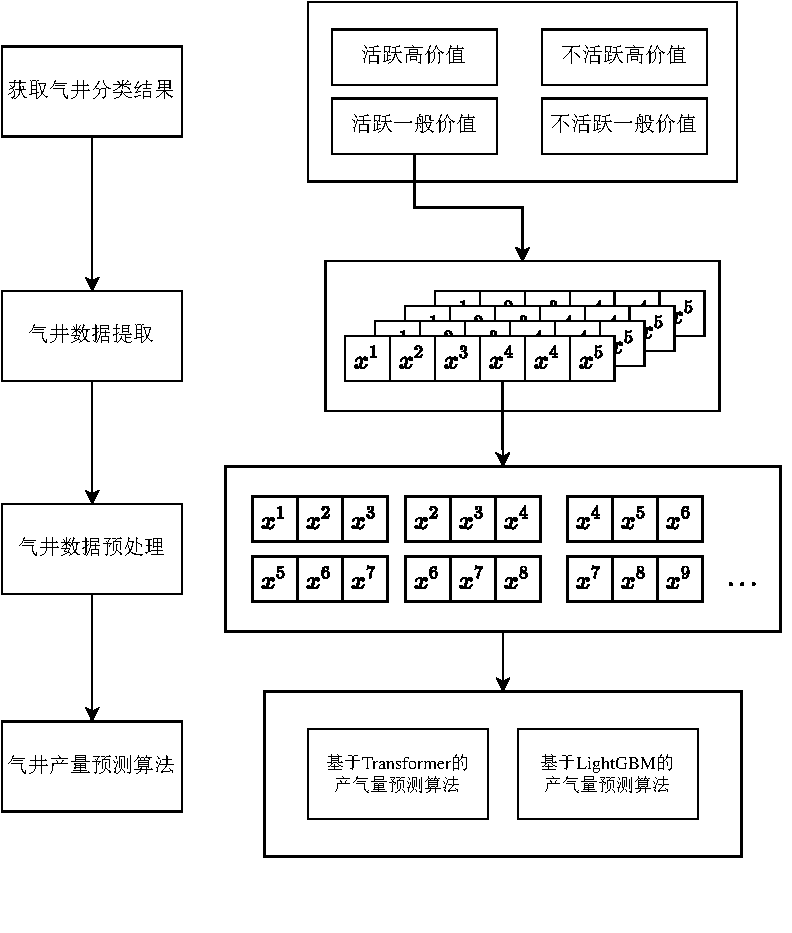
\includegraphics{figure/第四章框架图.vision.pdf}
    \caption{基于transformer的气井产量预测算法框架示意图}
    \label{fig:TFTprogess}
\end{figure}

\section{基于transformer的气井产量预测算法}

\subsection{数据处理及分类}
\label{sec:datafoc}
气井的数据为第\ref{cha:data}章进行处理后的数据。

为了统一输入输出格式,
降低模型复杂度和计算开销,本文使用滑动窗口技术将
训练数据切割为固定长度。滑动窗口模式是进行序列预测问题处理的最常用的方式,通过控制窗口的大小,可以调整参与预测的历史数据的数量。其模型如
图\ref{fig:slidewindow}所示。
\begin{figure}[H]
    \centering
    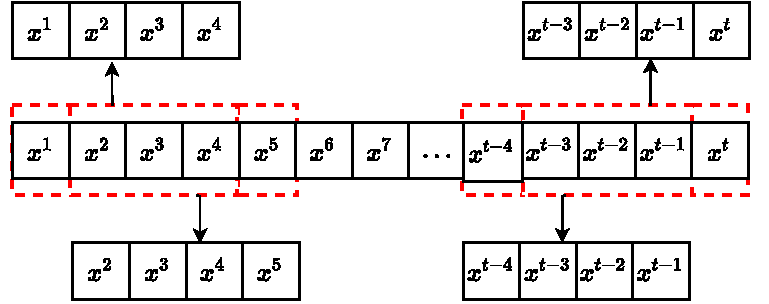
\includegraphics{figure/滑动窗口.vision.pdf}
    \caption{滑动窗口数据分段示意图}
    \label{fig:slidewindow}
\end{figure}
如图\ref{fig:slidewindow}所示,本文将预测步长设置为$\varDelta$, 将滑动窗口长度设置为$s$,用户在训练过程中,可以根据自己的需要对气井的时间序列进行划分。在取出样本序列后,每个样本分段的数据差异大且复杂,
未经标准化处理的样本分段会导致机器学习模型的学习速度十分缓慢,甚至无法更新模型参数,需要对每个样本分段进行无量纲化处理,将所有特征放缩至$[0,1]$之间,即
\begin{equation}
    x'_i = \frac{x_i - \mu}{\sigma}
\end{equation}
其中$x'_i$为标准化后的分段,$\mu$为该分段的均值,$\sigma$为该分段的标准差。
\subsection{算法主要设计策略}
如图\ref{fig:TFT}所示,为基于Transformer的气井产量预测算法的模型结构图。

本文借鉴了TFT对变量处理的思路,根据气井不同的协变量,将输入的历史时刻和未来时刻的特征经过一系列变换,得到一个抽象的
表征,然后分别输入到Encoder和Decoder中。Encoder部分使用GRU网络来编码历史时刻的信息,输出一个固定长度的向量,表示整个历史序列的含义。
Decoder部分使用自注意力机制来解码未来时刻的预测值,每个预测值都是根据之前所有时刻的加权结果得到的。

由于输入与目标之间的关系是未知的,对于预测结果而言,到底需要什么程度的非线性处理是一项巨大的挑战。非线性层过多会出现梯度消失或梯度爆炸的问题,因此,有时
需要简化模型来处理问题。为了让模型只在需要的时候才灵活地应用非线性地方式处理数据,本文采用了门控残差网络(GRN)来处理数据。

在时间序列的数据中,重要的点例如异常、变化点或者周期性模式一般都是根据他们周围的值来识别的。通过编码时间序列能够在序列中记忆和使用先前的信息,增强局
部上下文,从而提高基于注意力架构模型的性能。本文将采用时间特征处理层GRU来进行时间序列编码,
相较于LSTM,其具有更简单的结构,它合并了LSTM的遗忘门和输入门,因此参数数量较少,在训练和推理过程中的计算效率更高,且其有更快的训练速度,。在本文数据集规模较大的情况下进行实验和调整参数时更加高效。

在进行GRU编码后,本文采用自注意力来学习不同时间步之间的长期关系。最终借鉴MQRNN框架\cite{wen2018multihorizon}的思路,本文采用分位数回归预测作为模型的输出方式。

\begin{figure}[H]
    \centering
    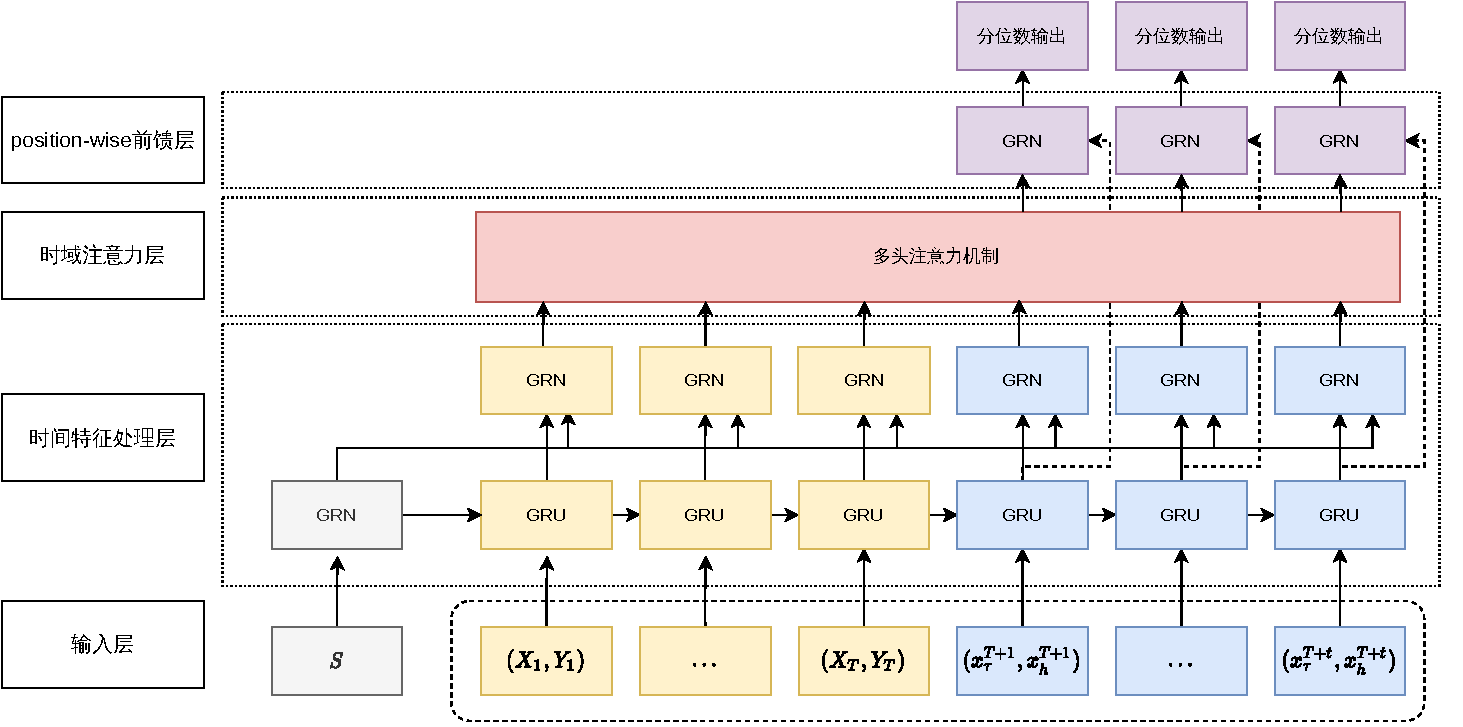
\includegraphics[width=.99\linewidth]{figure/基于Transformer的算法.vision.pdf}
    \caption{基于transformer的气井产量预测算法的模型结构图}
    \label{fig:TFT}
\end{figure}

综上所述,网络模型主要由门控残差网络、输入层、时间特征处理层、时域注意力层、position-wise前馈层以及分位数预测层组成具体如下:

(1) 输入层

本模型根据企业专家经验选取了多种数据并将他们融合。具体地由图中可知:输入层包括三种类型的变量。最左侧的$S$是静态变量,包括气井号$WellNO$、井丛号$cluster$和集气站号$Station$。从$(X_1, Y_1)$到$(X_{T}, Y_{T})$代表的是从过去时刻已知
,但未来不可知的随时间变化的变量,包括油压\( \delta \)、套压\( \rho \)、
井口温度\( \sigma \)和日产量$\varphi $。最右侧的$(x^{T+1}_{\tau }, x^{T+1}_{h })$到$(x^{T+t}_{\tau }, x^{T+t}_{h})$代表的是从过去$t-k$到未来$t+\tau_{max}$时刻
都可知的随时间变化的变量,包括已经如投产天数\( \tau \)、每日开井时间$h$等。

其中静态变量$S$需要经过静态协变量编码器来整合来自静态元数据的信息。具体地,本文使用上文采用的门控残差网络来编码产生上下文向量$\mathbf{c}_h$,$\mathbf{c}_e$
,$\mathbf{c}_h$将传入时间特征的局部处理层作为GRU的初始输入,$\mathbf{c}_e$可与进行时间特征编码后的动态变量一起进入GRN,流入多头注意力。

(2)门控残差网络

门控残差网络的输入为主输入$\mathbf{a}$
和一个可选的上下文向量$\mathbf{c}$。
其示意图如\ref{fig:GRN}所示。
\begin{figure}[H]
    \centering
    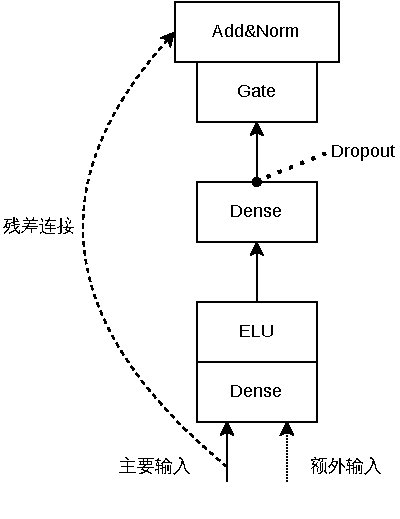
\includegraphics{figure/残差连接.vision.pdf}
    \caption{门控残差网络(GRN)示意图}
    \label{fig:GRN}
\end{figure}
具体操作如下所示:
\begin{equation}
    GRN_{\omega}(\mathbf{a}, \mathbf{c}) = \text{LayerNorm}(\mathbf{a} + GLU_{\omega}(\boldsymbol{\eta}_1))
\end{equation}
其中:
\begin{equation}
    \boldsymbol{\eta}_1 = \mathbf{W}_{1,\omega} \boldsymbol{\eta}_2 + \mathbf{b}_{1,\omega}
\end{equation}
\begin{equation}
    \boldsymbol{\eta}_2 = \text{ELU}(\mathbf{W}_{2,\omega} \mathbf{a} + \mathbf{W}_{3,\omega} \mathbf{c} + \mathbf{b}_{2,\omega})
    \label{eq:eta2}
\end{equation}
上式中,ELU是指线性激活函数,$\eta_1 \in \mathbb{R}^{d_{\text{model}}}$, $\eta_2 \in \mathbb{R}^{d_{\text{model}}}$ 是中间层,
LayerNorm是标准归一化,$\omega$ 是表示权重共享的索引。本文使用基于门控线性单元 (GLUs)的组件门控层来
控制非线性贡献的程度。假设 $\boldsymbol{\gamma } \in \mathbb{R}^{d_{\text{model}}}$ 是输入,GLU的形式为:
\begin{equation}
    GLU_{\omega}(\boldsymbol{\gamma }) = \sigma(\mathbf{W}_{4,\omega} \mathbf{\boldsymbol{\gamma }} + \mathbf{b}_{4,\omega}) \odot (\mathbf{W}_{5,\omega} \mathbf{\boldsymbol{\gamma }} + \mathbf{b}_{5,\omega}),
\end{equation}
其中 $\sigma(\cdot)$ 是sigmoid激活函数,$\mathbf{W}_{(\cdot)} \in \mathbb{R}^{d_{\text{model}} \times d_{\text{model}}}$ 是权重,$\mathbf{b}_{(\cdot)} \in \mathbb{R}^{d_{\text{model}}}$ 是偏置,
$\odot $ 是元素的Hadamard乘积。GLU允许模型控制GRN对原始输入$\mathbf{a}$的贡献程度:在必要的情况下,GLU的输出可以都接近于0,以便抑制模型非线性
的贡献。对于没有上下文向量$\mathbf{c}$的实例,GRN简单地将上下文输入视为0(即在\eqref{eq:eta2}中,$\mathbf{c}=0$)。

(3)局部时间特征处理

我们将过去的输入序列$\bm{\xi}_{1:T}$提供给编码器,将未来的输入序列$\bm{\xi}_{T+1:T+t}$
提供给解码器。使用GRU生成一组均匀的时间特征,作为下一阶段的输入,用$\phi (t,n)$来表示,
其中$\phi(t,n) \in {\phi(t, 1), \ldots, \phi(t, T+t)}$,$n$是位置指标。这种方式也可以完美处理观测到的过去和未来的输入不同而
存在的差异。同时,为了让静态数据也参与到时间序列变量的编码中,我们使用$\mathbf{c_h}$上下文向量初始化第一个GRU的隐藏状态。在此处也使用门控跳跃链接:
\begin{equation}
    \tilde{\bm{\phi}}(t, n) = \text{LayerNorm}\left(\tilde{\bm{\xi}}_{t+n} + \text{GLU}_{\phi}(\bm{\phi}(t, n))\right)
\end{equation}
其中$n \in [ -k, \tau_{\max}]$是位置指标。

为了让静态变量在模型中充分发挥作用,将静态变量和动态变量都经过GRN编码再送入时域注意力层,公式如\eqref{eq:staticencoder}层。
\begin{equation}
    \theta(t, n) = GRN_{\phi}(\hat{\phi}(t, n), c_e),
    \label{eq:staticencoder}
\end{equation}
其中$GRN_{\phi}$的权重在整个层中是共享的,$\mathbf{c}_e$是来自静态协变量得到的向量。

(4)时域注意力层

传统的多头注意力每个头使用不同的值,仅通过权重注意力本身并不能指示特定特征的重要性,此处
在传统多头注意力的基础上共享V。具体如下:
一般来说,注意力机制基于键矩阵\( K \in \mathbb{R}^{N \times d_{\text{attn}}} \)和查询矩阵\( Q \in \mathbb{R}^{N \times d_{\text{attn}}} \)
之间的关系对值\( V \in \mathbb{R}^{N \times d_v} \)进行缩放:
\begin{equation}
    \text{Attention}(Q, K, V) = A(Q,K)V
\end{equation}
其中$A()$是一个归一化函数,\( N \) 是进入注意力层的时间步数(即 \( k + t_{\text{max}} \))。常用的选择是缩放点积注意力:
\begin{equation}
    A(Q, K) = \text{Softmax}\left(\frac{QK^T}{\sqrt{d_{\text{attn}}}}\right)
\end{equation}
为了提高注意力机制的学习能力,Vaswani于2017年提出了多头注意力,使用不同的头针对不同的表示子空间:
\begin{equation}
    \text{MultiHead}(Q, K, V) = [H_1, \ldots, H_m]W_H
\end{equation}
\begin{equation}
    H_h = \text{Attention}(QW^Q_{(h)}, KW^K_{(h)}, VW^V_{(h)})
\end{equation}
其中\( W^K_{(h)} \in \mathbb{R}^{d_{\text{model}} \times d_{\text{attn}}} \), \( W^Q_{(h)} \in \mathbb{R}^{d_{\text{model}} \times d_{\text{attn}}} \), \( W^V_{(h)} \in \mathbb{R}^{d_{\text{model}} \times d_v} \) 
是针对键、查询和值的头特定权重 \( W_H \in \mathbb{R}^{m \cdot h \times d_{\text{model}}} \) 用于将所有头输出合并。
为了展示特定特征的重要性,做出的修改如下:
\begin{equation}
    \text{InterpretableMultiHead}(\mathbf{Q}, \mathbf{K}, \mathbf{V}) = \tilde{\mathbf{H}} \mathbf{W}_h
\end{equation}
\begin{equation}
    \begin{aligned}
        \mathbf{\tilde{H}} &= \tilde{A}(\mathbf{Q}, \mathbf{K}) \mathbf{V} \mathbf{W}_v, \\
        &= \left\{ \frac{1}{m_H} \sum_{h=1}^{m_H} A(\mathbf{Q} \mathbf{W}_Q^{(h)}, \mathbf{K} \mathbf{W}_K^{(h)}) \right\} \mathbf{V} \mathbf{W}_v, \\
        &= \frac{1}{m_H} \sum_{h=1}^{m_H} \text{Attention}(\mathbf{Q} \mathbf{W}_Q^{(h)}, \mathbf{K} \mathbf{W}_K^{(h)}, \mathbf{V} \mathbf{W}_v),
    \end{aligned}        
\end{equation}
式中:$\mathbf{W}_v \in \mathbb{R}^{d_{\text{model}} \times d_v}$是跨所有头共享的值的权重,$\mathbf{W}_h \in \mathbb{R}^{d_{\text{attn}} \times d_{\text{model}}}$
用于最终的线性映射。$\tilde{A}(\mathbf{Q}, \mathbf{K})$允许我们通过分析一组注意力权重来进行简单的可解释性研究。

在进行了时间特征处理层之后,我们应用注意力层。将所有的时间特征组合成单一的矩阵即$\bm{\varPhi }(t) = \left[ \bm{\theta} (t, -k), \ldots, \bm{theta }(t, \tau_{\text{max}}) \right]^T$
并在每个时间点($N = \tau _{max} + k + 1$)应用时域注意力:
\begin{equation}
    \mathbf{B}(t) = \text{InterpretableMultiHead}(\mathbf{\theta }(t), \mathbf{\theta }(t), \mathbf{\theta }(t)),
\end{equation}
生成了$\mathbf{B}(t) = \left[ \mathbf{\beta }(t, -k), \ldots, \mathbf{\beta }(t, \tau_{\max}) \right]$。在自注意力层之后,增加了一个额外
的门控层来促进训练:
\begin{equation}
    \boldsymbol{\delta}(t, n) = \text{LayerNorm}(\boldsymbol{\theta }(t, n)) + \text{GLU}_{\boldsymbol{\delta}}(\boldsymbol{\beta}(t, n)).
\end{equation}

(5)position-wise前馈层

对自注意力层应用额外的非线性处理,此处依然使用门控残差网络:
\begin{equation}
    \boldsymbol{\psi}(t, n) = \text{GRN}_{\boldsymbol{\psi}}(\boldsymbol{\delta}(t, n))
\end{equation}
其中$ \text{GRN}_{\boldsymbol{\psi}}$的权重在整个层中共享。此处还应用了一个跳过整个transformer块的残差连接,为序列到序列层提供了直接的路径。
倘若不需要额外的复杂性,就可以得到一个更简单的模型。如下所示:
\begin{equation}
    \tilde{\boldsymbol{\psi}}(t, n) = \text{LayerNorm}(\tilde{\boldsymbol{\delta}}(t, n)) + \text{GLU}_{\tilde{\boldsymbol{\psi}}}({\boldsymbol{\psi}}(t, n))
\end{equation}

\subsection{损失函数}

本文使用了分位数损失预测的方式。具体来说就是回归模型在对目标产量进行预测的时候不只预测$y$的一个期望值$\hat{y}$,
而是预测出$y$的概率分布中不同百分位数(如25\%,50\%,75\%)的值。分位数预测是根据上一步输出的线性变换生成的:
\begin{equation}
    \hat{\boldsymbol{y_i}}(q, t, \tau) = f_q (\tau, y_{i,1:T}, Z_{i,1:T}, X_{i,T:T+t}, S_i)
\end{equation}
其中,$\hat{\boldsymbol{y_i}}(q, t, \tau)$表示在时刻t,对未来$\tau$步进行预测的q分位数,$f_q(\cdot)$为预测模型,$ y_{i,1:T}$表示历史目标变量,$Z_{i,1:T}$表示过去已知,未来不可知的动态协变量,$X_{i,T:T+t}$表示过去未来都可知的动态协变量,$S_i$表示静态协变量。
本文采用联合最小化分位数损失来训练模型,并将所有的分位数方法相加,具体如式\eqref{eq:loss}所示。
\begin{equation}
    \mathcal{L}(\Omega, \mathbf{W}) = \sum_{y_t \in \Omega} \sum_{q \in \mathcal{Q} } \sum_{\tau=1}^{\tau_{\max}} \frac{\text{QL}(y_t, \hat{\boldsymbol{y}}(q, t - \tau, t), q)}{M_{\tau_{\max}}}
    \label{eq:loss}
\end{equation}
其中$\text{QL}(y,\hat{y},q)$为分位数损失,具体定义如下:
\begin{equation}
    \text{QL}(y, \hat{y}, q) = q(y - \hat{y})_+ + (1 - q)(\hat{y} - y)_+,
\end{equation}
在式\eqref{eq:loss}中,$\Omega$是包含M个样本的训练数据,$W$表示模型的权重,$\mathcal{Q}$是分位数的集合(用户可自行指定,本文使用$\mathcal{Q} = \{0.25,0.5,0.75\}$)。$\mathcal{L}(\Omega, \mathbf{W})$是平均单挑时序且平均预测点下的分位数损失。
由于$(\cdot)_+ = \max(0, \cdot)$,且$y-\hat{y}$与$\hat{y}-y$一定是一正一负,因此第二个公式可以转换为
\begin{equation}
    \text{QL}(y, \hat{y}, q) =  \max(q(y - \hat{y} ), (1 - q)(\hat{y} - y))
\end{equation}
假设拟合分位数0.75的目标值,代入公式即如式\eqref{eq:0.75}所示。
\begin{equation}
    \text{QL}(y, \hat{y}, q=0.75) =  \max(0.75(y - \hat{y} ), 0.25(\hat{y} - y))
    \label{eq:0.75}
\end{equation}
此时会有两种情况,若$(y - \hat{y} )$,即模型预测偏小,Loss增加会更多,否则模型预测偏大,Loss增加会更少。由于权重是3:1,所以训练时,模型会越来越趋向于预测出大的数字,这样Loss下降的更快,则模型的整个拟合的超平面会向上移动,
这样便能很好的拟合出目标变量的75分位数值。为了避免不同预测点下的预测量纲不一致问题,本文对随时函数进行了正则化处理。
\section{算法实现}
\subsection{基于transformer的气井产量预测算法}
\subsection{基于LightGBM的气井预测算法}
根据前文所述,本问题需要同时对1000余口气井构建时间序列预测模型,且问题包含多种类型的协变量,由第一章的国内外研究现状可知,机器学习模型中,当前对于时间序列预测问题的主流选择是特征工程+LightGBM模型的方法,这也是当前各大时间序列竞赛中大多数获胜方案所采用的策略。
下面将对LightGBM模型的设计做具体介绍。

决策树模型可以用于回归预测任务,其基本原理是将输入变量空间划分成多个子空间,并在每个子空间内拟合一个简单的回归模型。在预测时,将输入数据映射到对应的子空间,并用该子空间内的回归模型来进行预测,从而得到最终的预测结果。

集成树模型的原理是将多个弱学习器(例如决策树)组合成一个强学习器,从而提高预测的准确性和稳定性。在具体的实现中,集成树模型通常采用Bagging或Boosting的方法进行集成。其中Boosting是一种迭代式的方法,通过序列化训练多个决策树模型,每次训练的模型都会针对前一轮的错误进行优化,从而逐步提升模型的准确性。在Boosting中,还有一种著名的算法叫做梯度提升树(Gradient Boosting Tree),它通过在每轮迭代中拟合负梯度来进行模型训练。LightGBM(Light Gradient Boosting Machine)是一种基于决策树的梯度提升框架,是由微软亚洲研究院开发的。它具有高效性和准确性,尤其适用于处理大规模数据集。相较于其他梯度提升框架,LightGBM 在训练速度和内存使用方面具有优势。

多步时间序列预测是指根据历史数据来预测未来多个时刻的数据,例如预测未来一周的天气或销量。要使LightGBM模型适应于多步时间序列预测,需要进行以下几个步骤:

数据准备:对于本问题,需要将历史产气量数据按照气井号和时间顺序进行排序,并且将数据集划分为训练集,验证集和测试集。同时,需要对静态协变量和随时间变化的协变量进行特征工程处理。
数据准备过程分为数据清洗和数据划分,数据清洗如\ref{cha:data}所述,数据划分部分选取每口井最后一段forecast horizon长度的气井产量数据作为测试集(forecast horizon指要预测的长度,如对未来45天的每日产气量进行
预测),选取倒数第二个forecast horizon长度的气井产量数据作为验证集,验证集用来调整lightGBM模型的超参数,其余数据用作测试集。

对时间序列数据进行特征工程,抽取延迟特征、滑动窗口特征等。在该问题中,所选取的静态特征包括,集气站号Station,井丛号Cluster,气井号WellNo,配产量Allocation,其余特征包括表示时间的整数Elapsed,这个整数值通过当前日
期与数据集第一天的日期差计算得到,表示气井生产时长的整数值ElapsedProduction,通过当前日期与气井投产日期的日期差计算得到,当日开井时间DailyHour,延迟特征Lag1到Lag30,其中延迟特征Lagi表示当前日期前i天的产气量,即使
用过去的产气量数据预测未来产气量(这里以预测未来7天的产气量为例,使用过去30天的数据预测未来7天的产气量),滑动特征RollingMean7,RollingStd7,……,RollingMean180, RollingStd180,其中RollingMeani和RollingStdi分
别表示过去i天产气量数据的均值和方差,i取{7,15,30,60,180},通过Rolling特征提取历史产气量数据的数值信息。这里具体使用过去多长时间的历史数据对未来进行预测通常根据经验选取,通常这个长度在forecast horizon到2*forecast horizon之间。
进行特征工程后,构造训练数据,将每个时刻的产气量作为目标值和对应的特征作为一条样本,具体如表\ref{tab:asamplefeature}所示。
\begin{table}[H]
    \renewcommand{\arraystretch}{1.5}
    \centering
    \caption{一条样本所包含的特征}
    \label{tab:asamplefeature}
    \begin{tabular}{|c|c|c|c|c|c|c|c|}
        \hline
        名称 & 集气站号 & 井丛号 & 气井号 & 配产量 & 所有时间长度 & 投产时长 & 当日开井时间 \\
        \hline
        特征 & Station & Cluster & WellNo & Allocation & Elapsed & ElapsedProduction & DailyHour\\
        \hline
        名称 & \multicolumn{2}{c|}{前i天产气量} & \multicolumn{5}{c|}{滑动特征}     \\
        \hline
        特征 & \multicolumn{2}{c|}{Lag{i}} & \multicolumn{5}{c|}{RollingMean{i}, RollingStd{i}}\\
        \hline
    \end{tabular}
\end{table}
表\ref{tab:singlesamp}表示一条训练样本(再加上进行特征工程Lag和Rolling特征),DailyProduction表示当日产气量,为目标值。
\begin{table}[H]
    \renewcommand{\arraystretch}{1.5}
    \centering
    \caption{单条样本示意表}
    \label{tab:singlesamp}
    \begin{tabular}{|c|c|c|c|c|c|c|c|}
        \hline
        Station & Cluster & WellNO & Elapsed & ElapsedProduction &Allocation & DailyHour & DailyProduction \\
        \hline
        X5 & 997 & XE2213-HU9 & 1 & 1& 10.0000 & 3.60000 & 1.40000 \\
        \hline
    \end{tabular}
\end{table}
调整LightGBM模型的参数,根据不同
的目标函数、评价指标、学习率、树的深度、叶子节点数等进行手动或自动调优。最终模型选择超参数如表\ref{tab:LightGBMSuper}所示,使用huber损失函数,MAE作为指标来对模型预测效果拟合效果进行评价。
\begin{table}[H]
    \renewcommand{\arraystretch}{1.5}
    \centering
    \caption{基于LightGBM的气井预测算法超参数}
    \label{tab:LightGBMSuper}
    \begin{tabular}{|c|c|c|c|c|c|c|}
        \hline
        Name & boosting\_type & objective & metric & min\_data\_in\_leaf & max\_depth & subsample \\
        \hline
        Value & gbdt & huber & mae & 20 &8 & 0.8 \\
        \hline
        Name & colsample\_bytree & learning\_rate & max\_bin & n\_estimators & boost\_from\_average & verbose \\
        \hline
        Value & 0.8 & 0.05 & 1000 & 3000 & True & -1 \\
        \hline
    \end{tabular}
\end{table}
其中huber损失函数的定义如式\eqref{eq:huber}所示。
\begin{equation}
    L_{\delta}(y, f(x)) = 
        \begin{cases} 
        \frac{1}{2}(y - f(x))^2, & \text{if } |y - f(x)| \leq \delta \\
        \delta|y - f(x)| - \frac{1}{2}\delta^2, & \text{if } |y - f(x)| > \delta
        \end{cases}
    \label{eq:huber}
\end{equation}
在中,\(f(x)\)为预测值,δ为Huber损失函数的参数,δ接近0时,
Huber损失趋向于MAE。δ越大时,Huber损失趋向于MSE,在梯度下降时 MSE较MAE更为准确。而在异常值出现时 MAE较MSE更加鲁棒。Huber损失函数集中了两者的优势。这里MAE损失的定义如式\eqref{eq:Maeloss}所示。
\begin{equation}
    MAE = |y - f(x)|
    \label{eq:Maeloss}
\end{equation}

MSE损失的定义如式\eqref{eq:mseloss}所示。
\begin{equation}
    MSE = (y - f(x))^2
    \label{eq:mseloss}
\end{equation}

确定训练样本和模型超参数后,即可进行LightGBM模型的训练过程。在推理阶段,使用训练好的模型对于任一指定气井未来一段时间内的单日产气量做出预测。

在训练好的模型中,通过递归预测的方式,预测未来若干天的产气量。具体地,从当前时刻开始,先用模型预测未来第一天的产气量,然后将预测结果作为已知量(未来第二天地Lag1特征)输入到模型中,再预测未来第二天的产气量,以此类推。
\section{实验对比分析}
\subsection{数据集描述与环境说明}
基于transformer的气井产量预测算法会在第\ref{sec:datafoc}节提供的数据集上进行验证。本次实验的硬件环境为处理器Inter(R) Xeon(R) Silver 4261 cpu @ 2.10Hz,
显卡GeForce RTX 3090,内存256G,磁盘1T,操作系统采用Windows 10,开发环境为Pycharm,Python环境为Anaconda-4.12.0 python=3.9。
\subsection{评估指标}
为了验证本章所提出的基于transformer的气井产量预测算法的有效性,使用两个指标用于评估。其中一个是平均绝对误差(Mean Absolute Error, MAE),其可以衡量
预测值与实际值之间的平均绝对偏差。公式如式\eqref{eq:MAE}所示。
\begin{equation}
    MAE(y, y') = \frac{1}{n} \sum_{i=1}^{n} |y_i - y'_i|
    \label{eq:MAE}
\end{equation}
另一个常用误差指标为累计产量的相对误差,公式如式\eqref{eq:RCPE}所示。
\begin{equation}
    RCPE = \frac{\sum_{i=1}^{n} |y_i| - \sum_{i=1}^{n} |y'_i|}{\sum_{i=1}^{n} |y_i|}
    \label{eq:RCPE}
\end{equation}
上面两式中,$i$表示索引,用于遍历数据集中的每一个数据点。例如,如果我们有一个包含多个观测值的数据集,$i$就用来表示这些观测值的序号,从第一个观测值
到第$n$个观测值。$y$表示真实值,也就是实际产量,$\hat{y}$表示预测值,也就是通过模型预测得到的产量。
\subsection{对比实验}
(1) 对比模型选择
根据前文所述,本问题需要同时对1000余口气井构建时间序列预测模型,且问题包含多种类型的协变量,因此初步选取基于注意力机制的seq2seq模型,lightGBM模型、TFT模型以及本文的模型这四个可以解决这类问题的模型进行实验。

经过对手头的单井日报数据进行处理,累计10年,1000余口气井约有总共约有160多万条数据。为了展示各算法的预测性能,选出3口井的产量数据作为测试集进行测试,分别是:SN0016-05, SN0004-04,SN0012-10。这3口井的近期
平均产量分别位于大于2,1到2之间,小于1区间(单位:$10^4m^3$).如表\ref{fig:modelselection}所示,基于注意力机制的seq2seq模型,由于模型结构限制,无法包含未来时刻的开关井信息,导致预测效果显著劣于其余三个模型。
lightGBM模型、TFT模型及本模型,预测准确率相近,本文算法略优于TFT和lightGBM模型,预测时间本文模型优于TFT和lightGBM模型。但是在模型训练阶段,lightGBM模型(10min)显著快于TFT模型(4h)及本文(2.5h)。故最终保留
本文中的模型和lightGBM模型。
\begin{table}[H]
    \renewcommand{\arraystretch}{1.5}
    \caption{模型选择实验结果}
    \label{fig:modelselection}
    \centering
    \begin{tabular}{|c|c|c|c|c|}
        \hline
        \textbf{测试对象} & \textbf{模型} & \textbf{MAE($10^4 \ m^3$)} & \textbf{RCPE(\%)} & \textbf{预测时间(s)} \\ \hline
        \multirow{4}{*}{SN0016-05}  & TFT          & 0.241                       & 3.14              & 8.369                \\ \cline{2-5}
                                    & LightGBM     & 0.262                       & 3.80              & 0.89                 \\ \cline{2-5}
                                    & Seq2seq      & 0.512                       & 10.25             & 5.25                 \\ \cline{2-5}
                                    & Ours         & 0.225                       & 3.02              & 7.29                 \\ \hline
        \multirow{4}{*}{SN0004-04}  & TFT          & 0.041                       & 1.39              & 12.9                 \\ \cline{2-5}
                                    & LightGBM     & 0.043                       & 1.40              & 0.92                 \\ \cline{2-5}
                                    & Seq2seq      & 0.132                       & 7.89              & 6.22                 \\ \cline{2-5}
                                    & Ours         & 0.036                       & 1.36              & 12.1                 \\ \hline
        \multirow{4}{*}{SN0012-10}  & TFT          & 0.103                       & 24.8              & 13.52                \\ \cline{2-5}
                                    & LightGBM     & 0.112                       & 27.0              & 1.03                 \\ \cline{2-5}
                                    & Seq2seq      & 0.153                       & 30.1              & 6.34                 \\ \cline{2-5}
                                    & Ours         & 0.095                       & 24.1              & 13.16                \\ \hline
    \end{tabular}
\end{table}
结合图中可以看出,本文的模型在MAE和RCPE指标上的表现均优于其他三种模型,TFT由于参数量太复杂训练和预测时间都较久,效果也稍次于本模型。相对而言,LightGBM模型预测时间较短且也可以取得相对较好的预测结果。
这表明在实时性要求较高的场景中,LightGBM模型可能是一个较好的选择。Seq2seq模型在这三个测试对象上的表现相对较差,可能需要进一步优化模型结构或参数。根据实验结果,可以得出结论:在这三个测试对象上,本模型的预测性能最佳,
但预测时间较长。当实时性要求较高时,可以考虑使用LightGBM模型。

(2)使用部分数据进行预测

本次实验的动机为:由于早期数据缺乏套压记录,这可能会影响预测模型的准确性。近期数据包含了所有重要特征,包括套压数据,并且能够代表整个时间序列的主要趋势和模式,那么只使用近期数据进行预测可能是一个合理的选择。
\begin{table}[h]
    \renewcommand{\arraystretch}{1.5}
    \centering
    \caption{使用部分数据集训练和使用全数据集训练的对比}
    \label{tab:alldatacomparison}
    \begin{tabular}{|c|c|c|c|c|}
    \hline
    \textbf{气井产量区间($10^4 \ m^3$)} & \multicolumn{2}{c|}{\textbf{MAE}} & \multicolumn{2}{c|}{\textbf{RCPE}} \\ 
    \cline{2-5} 
    \textbf{(}$10^4 m^3$\textbf{)} & 使用部分数据 & 使用全部数据 & 使用部分数据 & 使用全部数据 \\ 
    \hline
    大于4               & 0.267        & 0.367        & 0.022        & 0.051        \\ 
    \hline
    3至4               & 0.193        & 0.249        & 0.028        & 0.048        \\ 
    \hline
    2至3               & 0.136        & 0.130        & 0.042        & 0.042        \\ 
    \hline
    1至2               & 0.101        & 0.103        & 0.047        & 0.042        \\ 
    \hline
    小于1               & 0.120        & 0.122        & 0.165        & 0.163        \\ 
    \hline
    \end{tabular}
\end{table}
为对比预测效果,使用本文模型针对未来7天的产气量构建预测模型,分别使用所有数据和使用2017-01-01之后的数据构建两个不同的模型。根据近期平均产量将所有井划分为大于4,3到4之间,2到3之间,1到2之间,小于1这五类,每类类
别数分别为23,41,85,198,620.使用两种模型对这5类型的气井分别进行预测,要计算的预测准确性指标包括MAE(平均绝对误差)和RCPE(相对百分比误差)。对每类型井的预测指标进行统计,使用预测指标在每类型气井的中位数作为对
该类预测效果的近似表示。在测试过程中,存在部分井由于开井时间较晚,数据数小于时间序列预测的时间窗口,需对这部分井进行排除,此外,一些井在预测时间段内由于均处于关井状态,产气量为0,这部分井的预测缺乏统计学意义,同样予
以排除。
    
通过对每类型气井的预测指标进行统计,可以得出以下结论:

对于产量大于4的气井,使用2017-01-01之后的数据预测的MAE为0.267,而使用所有数据的MAE为0.367。同时,RCPE分别为0.022和0.051。这说明基于2017-01-01之后的数据构建的模型预测效果较好。对于产量在3到4之间的气井,使
用2017-01-01之后的数据预测的MAE为0.193,而使用所有数据的MAE为0.249。同时,RCPE分别为0.028和0.048。这同样说明基于2017-01-01之后的数据构建的模型预测效果较好。对于产量在2到3之间的气井,MAE和RCPE分别
为0.136、0.130和0.042、0.042。在这个区间,两个模型的预测效果相当。对于产量在1到2之间的气井,使用2017-01-01之后的数据预测的MAE为0.101,而使用所有数据的MAE为0.103。同时,RCPE分别为0.047和0.042。在这个区间,两个
模型的预测效果相当,但基于2017-01-01之后的数据构建的模型在MAE上略好。对于产量小于1的气井,使用2017-01-01之后的数据预测的MAE为0.120,而使用所有数据的MAE为0.122。同时,RCPE分别为0.165和0.163。在这个区间,两个模
型的预测效果相当,但基于所有数据构建的模型在RCPE上略好。

综上所述,在大部分产量区间中,基于2017-01-01之后的数据构建的模型预测效果都较好,但在产量较低的区间中,两个模型的预测效果相当。

(3)本模型和LightGBM模型对比

实验基本设置: 在这个实验中,我们选用本模型和LightGBM(一种基于梯度提升决策树的机器学习模型)对未来7天的产气量进行预测。实验结果是对属于该日均产气量范围内的所有气井进行预测并计算其指标的中位数统计值得到的。
\begin{table}[H]
    \renewcommand{\arraystretch}{1.5}
    \centering
    \caption{本文模型和LightGBM模型预测结果对比}
    \label{tab:prediction_comparison}
    \begin{tabular}{|c|c|c|c|}
    \hline
    模型     & 预测时间区间 & MAE($10^4 m^3$) & RCPE(\%) \\ \hline
    LightGBM & 小于 1      & 0.128           & 0.228    \\ \hline
    LightGBM & 1 到 2      & 0.136           & 0.093    \\ \hline
    LightGBM & 大于 2      & 0.149           & 0.043    \\ \hline
    Ours      & 小于 1      & 0.122           & 0.163    \\ \hline
    Ours      & 1 到 2      & 0.102           & 0.047    \\ \hline
    Ours      & 大于 2      & 0.163           & 0.035    \\ \hline
    \end{tabular}
\end{table}
实验结果对比与分析: 根据上述统计结果表格,可以看出:

对于日均产气量小于1的气井,本文模型的MAE和RCPE分别为0.122和0.163,而LightGBM模型分别为0.128和0.228。在这种情况下,本文模型的预测性能更好。

对于日均产气量在1到2之间的气井,本文模型的MAE和RCPE分别为0.102和0.047,而LightGBM模型分别为0.136和0.093。在这种情况下,本文模型的预测性能也更好。

对于日均产气量大于2的气井,本文模型的MAE和RCPE分别为0.163和0.035,而LightGBM模型分别为0.149和0.043。在这种情况下,尽管本文模型在RCPE上的表现更好,但在MAE上,LightGBM模型的表现更优。

实验中对于日产量大于2的气井,选取123口井的测试结果作为有效数据,对于日产气量在1到2之间的气井,选取184口井的测试结果作为有效数据,对于日产气量小于1的气井,选取459口井的测试结果作为有效数据。

从预测性能上看,本文模型在各种情况下都表现出较好的预测性能。然而,从实用性的角度来看,LightGBM模型的训练和预测时间要远远低于本文模型。具体来说,LightGBM模型的重训练时间为5分钟,而本文模型为1.5小时;LightGBM模型
的预测时间平均约为1.2秒,而本文模型平均约为7.5秒。这意味着,在实际应用中,使用LightGBM模型会更加节省时间和计算资源。

总结:从实验结果来看,本文模型在预测性能上具有优势,但在实用性方面,LightGBM模型具有更好的表现。因此,在实际应用中,需要根据实际需求的精度和计算资源进行权衡,选择合适的模型。
\subsection{实验结果统计值展示}
为完整展示实验结果,分别列出两种预测模型分别在预测步长为7天和45天时的预测结果统计指标,统计指标不仅包括中位数,还包括平均数,\%25分位数,75\%分位数,标准差。
产量区间小于1、1到2、大于2三种类型测试气井数量分别为123、184、459。预测步长7天的MAE结果如表\ref{tab:MAE7}所示。
\begin{table}[H]
    \renewcommand{\arraystretch}{1.5}
    \centering
    \caption{本文模型和LightGBM模型预测未来7天内产气量预测结果的MAE指标对比}
    \label{tab:MAE7}
    \begin{tabular}{|c|c|c|c|c|c|c|}
    \hline
    模型     & 预测时间区间 & MAE mean & MAE std & MAE 25\% & MAE 50\% & MAE 75\% \\ \hline
    LightGBM & 小于 1      & 0.199    & 0.221   & 0.055    & 0.128    & 0.277    \\ \hline
    LightGBM & 1 到 2      & 0.180    & 0.179   & 0.069    & 0.136    & 0.211    \\ \hline
    LightGBM & 大于 2      & 0.249    & 0.286   & 0.087    & 0.149    & 0.297    \\ \hline
    Ours      & 小于 1      & 0.174    & 0.274   & 0.067    & 0.122    & 0.205    \\ \hline
    Ours      & 1 到 2      & 0.170    & 0.220   & 0.061    & 0.102    & 0.186    \\ \hline
    Ours      & 大于 2      & 0.300    & 0.454   & 0.089    & 0.163    & 0.298    \\ \hline
    \end{tabular}
\end{table}
预测步长7天的RCPE结果如表\ref{tab:RCPE7}所示。
\begin{table}[H]
    \renewcommand{\arraystretch}{1.5}
    \centering
    \caption{本文模型和LightGBM模型预测未来7天内产气量预测结果的RCPE指标对比}
    \label{tab:RCPE7}
    \begin{tabular}{|c|c|c|c|c|c|c|} % Change 'l' to 'c' for center alignment
    \hline
    模型     & 预测时间区间 & RCPE mean & RCPE std & RCPE 25\% & RCPE 50\% & RCPE 75\% \\ \hline
    LightGBM & 小于 1      & 0.433     & 0.845    & 0.097     & 0.228     & 0.477     \\ \hline
    LightGBM & 1 到 2      & 0.131     & 0.147    & 0.038     & 0.093     & 0.167     \\ \hline
    LightGBM & 大于 2      & 0.085     & 0.125    & 0.020     & 0.043     & 0.094     \\ \hline
    Ours      & 小于 1      & 0.363     & 0.757    & 0.066     & 0.163     & 0.358     \\ \hline
    Ours      & 1 到 2      & 0.112     & 0.187    & 0.016     & 0.047     & 0.098     \\ \hline
    Ours      & 大于 2      & 0.086     & 0.147    & 0.015     & 0.035     & 0.080     \\ \hline
    \end{tabular}
\end{table}
预测步长45天的MAE结果如表\ref{tab:MAE45}所示。
\begin{table}[H]
    \renewcommand{\arraystretch}{1.5}
    \centering
    \caption{本文模型和LightGBM模型预测未来45天内产气量预测结果的MAE指标对比}
    \label{tab:MAE45}
    \begin{tabular}{|c|c|c|c|c|c|c|}
    \hline
    模型       & 预测时间区间 & MAE mean & MAE std & MAE 25\% & MAE 50\% & MAE 75\% \\ \hline
    LightGBM  & 小于 1      & 0.198    & 0.151   & 0.091    & 0.159    & 0.273    \\ \hline
    LightGBM  & 1 到 2      & 0.245    & 0.191   & 0.106    & 0.186    & 0.306    \\ \hline
    LightGBM  & 大于 2      & 0.360    & 0.329   & 0.151    & 0.253    & 0.418    \\ \hline
    Ours       & 小于 1      & 0.132    & 0.113   & 0.058    & 0.110    & 0.181    \\ \hline
    Ours       & 1 到 2      & 0.217    & 0.207   & 0.077    & 0.130    & 0.272    \\ \hline
    Ours       & 大于 2      & 0.346    & 0.319   & 0.111    & 0.245    & 0.459    \\ \hline
    \end{tabular}
\end{table}
预测步长45天的RCPE结果如表\ref{tab:RCPE45}所示。 
\begin{table}[H]
    \renewcommand{\arraystretch}{1.5}
    \centering
    \caption{本文模型和LightGBM模型预测未来45天内产气量预测结果的RCPE指标对比}
    \label{tab:RCPE45}
    \begin{tabular}{|c|c|c|c|c|c|c|}
    \hline
    模型       & 预测时间区间 & RCPE mean & RCPE std & RCPE 25\% & RCPE 50\% & RCPE 75\% \\ \hline
    LightGBM  & 小于 1      & 0.384     & 0.750    & 0.089     & 0.201     & 0.396     \\ \hline
    LightGBM  & 1 到 2      & 0.117     & 0.121    & 0.029     & 0.074     & 0.160     \\ \hline
    LightGBM  & 大于 2      & 0.091     & 0.107    & 0.028     & 0.056     & 0.114     \\ \hline
    Ours       & 小于 1      & 0.361     & 1.731    & 0.071     & 0.146     & 0.319     \\ \hline
    Ours       & 1 到 2      & 0.112     & 0.128    & 0.026     & 0.072     & 0.146     \\ \hline
    Ours       & 大于 2      & 0.087     & 0.094    & 0.019     & 0.047     & 0.120     \\ \hline
    \end{tabular}
\end{table}
为直观展示预测结果,随机选择5口气井的预测结果如下文所示。
\section{开关井推荐}
本小节将介绍开关井策略推荐实际问题的解决办法。首先收集数据,包括井口产气量、井底压力、温度、环境温度、气价、能源成本等相关参数。同时也需
要采集各个气井的位置和特征等信息,以便进行搜索和选择。其次,根据实际情况和目标函数,选择合适的搜索算法。常见的搜索算法包括深度优先搜索、蚁群算法等。
不同算法有不同的优缺点,需要根据实际情况进行评估和选择。然后确定搜索空间,搜索空间即可选取的所有井的集合,需要考虑到可行性和搜索效率的平衡。通常可
以根据实际条件和目标函数,设置一些限制条件来缩小搜索空间,以提高搜索效率。接下来要执行搜索算法,根据设定的搜索算法,对搜索空间进行搜索。在搜索过程
中,需要按照目标函数的要求,评估不同井进行开关的效果,并记录每次开关井的结果和成本。在搜索完成后,需要对所有开关井的结果进行评估,选取最优的开关井方案。
评估时需要考虑到产量、成本、环境、管网模型等多方面因素,并综合权衡不同因素的影响,以选取最优的开关井方案。最后根据最优的开关井方案,实施相应的开关井策略。

气井开采过程中,通常会产生一定量的液体,包括水和油。产液量的增加会影响气井的产气量,因为液体在井筒中的积累会增加井筒的阻力,使气流的速度降低,
从而影响气井的产气量。当气井处于低压低产阶段时,气相不能有效地携带液体,会导致积液现象。此时,如采用间歇生产方式(即周期性地开关井),可以利用
关闭期间积累的压力差,在开启时将积聚在底部或中部的液体迅速排出。
但如果开关频率过高或关闭时间过短,则可能造成反复积排液、增加摩阻损失、降低生产效率。可若是开关频率过低或关闭时间过长,则可能导致底部水锥突
破、增加水含率、降低天然气质量。
\subsection{数据}
本小节使用过去三十天的井口温度、压力、开关井时间、产气量值并借助前文训练的产气量模型来预测未来七天内每口井的预计产气量;本文使用前一天的井口温度、压力以
及井丛的拓扑关系图等数据构建管网模型,计算压力差;通过对过去一段时间历史数据的总结得到每口井的开关井周期。
\subsection{算法设计}

(1)管网模型

在处理复杂的地下流体动力学问题时,精确的解析解往往难以获得。在某些情况下,特别是考虑到地层的渗透性、流体的粘度以及井筒和储层之间的压力交互作用时,压力沿
井深的变化近似于二次曲线。此处在计算平均压力时根据此理论采用了一个简化的假设,即压力分布沿井深呈二次曲线分布。在这个假设下,可以通过连接干管井丛的井口压
力平均值(P1)和管道出口压力,即集气站进站压力(P2)计算出平均压力(avgPressure)。具体公式如式\eqref{eq:avgPressure}所示。
\begin{equation}
    \text{avgPressure} = \frac{2.0 \times (P1^3 - P2^3)}{3.0 \times (P1^2 - P2^2)}
    \label{eq:avgPressure}
\end{equation}
式中,P1 和 P2 分别代表两个不同深度的压力值。

本文使用了一种经验模型来计算临界温度(Tpc)和临界压力(Ppc)。这个模型是基于大量实验数据得出的,它将气体相对密度($\delta$ )作为输入参数。
\begin{equation}
    T_{pc} = 93.3 + 181 \times \delta - 7 \times \delta^2
\end{equation}
\begin{equation}
    P_{pc} = 4.668 + 0.103 \times \delta - 0.259 \times \delta^2
\end{equation}
式中的气体相对密度$\delta$的默认取值为0.5962(无量纲)。

将实际温度(K)和平均压力(avgPressure)分别除以临界温度(Tpc)和临界压力(Ppc),得到温度和压力的缩减值(即相对于临界温度和临界压力的温度和压力)Tr和Pr。
\begin{equation}
    T_r = \frac{K}{T_{pc}}
\end{equation}
\begin{equation}
    P_r = \frac{\text{avgPressure}}{P_{pc}}
\end{equation}
式中K为开尔文温度$K = C + 273.15$。

压缩因子(Z-factor)是一个描述气体实际体积与理论(理想气体状态下的)体积之比的参数,是用于石油和天然气工程中评估气体的压缩性质的重要工具。压缩因子的值表明了实际气体与理想气体状态方程之间的偏离程度。

赞达尔方程\cite{Dranchuk1975CalculationOZ}(也称为Dranchuk-Aboukassem方程),是一种基于实验数据得出的经验公式,用于计算特定条件下的气体压缩因子。这个方程考虑了温度和压力的缩减值。具体公式如式\eqref{eq:Z-factor}所示。
\begin{equation}
    Z = 1 - \frac{3.52 \times P_r}{10^{0.9813T_r}} + \frac{0.274 \times P_r \times P_r}{10^{0.8157T_r}}
    \label{eq:Z-factor}
\end{equation}
通过使用该方程,可以在已知缩减温度和缩减压力的情况下,估计出天然气在特定温度和压力条件下的压缩因子,进而帮助工程师们更准确地预测和计算气体的行为和性能。
本式对于理解和计算实际天然气在地下储藏和输送过程中的物理行为至关重要。它使工程师能够更好地设计和优化天然气的提取、处理和运输系统。

最后,可以使用Darcy-Weisbach方程\cite{brown2002history}来计算压力。这个方程描述了气体在管道中流动时,由于摩擦损失而引起的压力降。在这里,需要考虑到气体的压缩性,因此使用压缩因子(Z)来修正方程。
\begin{equation}
    \text{calP1} = \left(P2^2 + 3.948 \times 10^{-8} \times Q \times Q \times \delta \times K \times \frac{L}{d^{1.6}}\right)^{0.5}
\end{equation}
此处Q代表产气量,单位为万方/日,在计算中需要进行单位换算。d是气井的管径,单位为毫米,默认取值为20。
当应用场景为气井传输管道(从井丛传输至集气站)时,$calP1$和$P1 - calP1$具有以下实际意义。

$calP1$:这个值表示计算得到的管道起点(如单口气井)的压力。它反映了在给定的生产条件(温度、产气量等)以及管道参数(长度、直径等)下,为了克服管道摩擦损失所需要的起始压力。 

$P1 - calP1$:这个值表示实际管道起点压力(P1)与计算得到的起点压力($calP1$)之间的差值。这个差值可以用来评估管道的性能和系统效率。以下是几种可能的情况:

当$P1 - calP1$接近于零时,表示实际压力和计算压力非常接近,说明管道系统运行良好,摩擦损失在可接受范围内。 

当$P1 - calP1$为正值时,表示实际起点压力高于计算压力。这可能意味着管道系统存在过高的摩擦损失或是管道中存在堵塞等异常现象。 

当$P1 - calP1$为负值时,表示实际起点压力低于计算压力。这可能意味着管道系统效率较高,但也可能导致管道中的气体流量不足,从而影响到集气站的运行。 

通过分析$calP1$和$P1 - calP1$这两个值,可以为气井生产提供有用信息,有助于对生产参数进行调整和优化,提高气井生产效率和安全性。同时,这些信息也可以用于诊断管道系统是否存在异常,以便及时采取纠正措施。

(2)搜索算法

基于对实际问题的分析,借助FOA算法来完成搜索。
主要对FOA算法中的距离进行了自定义:

当目前产量$current\_amount>target$(预计想要达到的总产量),系统需要从开着的井中选择一口井关闭,这时认为距离函数与压力差$delta\_pressure$和已经开井时间$open\_time$高度相关,因此距离函数定义如\eqref{eq:closewell}所示。
\begin{equation}
    \text{Dist}_i = \frac{1}{\sqrt{{\text{delta\_pressure}_i}^2 + {\text{open\_time}_i}^2}}
    \label{eq:closewell}
\end{equation}
当目前产量$current\_amount<target$时,系统需要从可以开的井中选择一口井打开,本文认为压力差越小越好,产气量越大越好,因此距离函数与产气量、压力差有关,距离函数的定义如如\eqref{eq:openwell}
\begin{equation}
    \text{Dist}_i = \frac{\sqrt{{\text{delta\_pressure}_i}^2}}{\sqrt{{\text{pre\_production}_i}^2}}
    \label{eq:openwell}
\end{equation}
将当前问题代入到果蝇优化算法具体的步骤如\ref{al:openwell}所示。
\begin{algorithm}[H]
    \caption{基于果蝇优化的开关井推荐算法}
    \begin{algorithmic}[1]
       \Require 目标产气量target区间,前一天的开关井情况
       \Ensure  新的开关井策略
       \State 初始化,以第一天的开关井情况作为初始值 init()
       \While{true}
            \If{current\_amount $>$ target}
                \State 随机分配方向、距离,搜索出一定数量可以关的井 update()
            \ElsIf{current\_amount $<$ target}
                \State 随机分配方向、距离,搜索出一定数量可以开的井 update()
            \Else
                \State \Return 最终开关井策略
            \EndIf
            \State 计算自定义的种群适应度
            \State 果蝇位置更新
        \EndWhile
    \end{algorithmic}
    \label{al:openwell}
\end{algorithm}

(3)搜索空间

在实际生产过程中,不是所有的关着井都可以开,需要动态的挑出这些可以开的井。根据分析,本文排除下面这些井,在这个周期不投入生产。

1.去除用户前端自定义输入的尚不参与生产的井;

2.根据历史数据计算开关井周期,如果某口井当前已经开井时间大于最大开井时间,则排除这口井;

3.基于管网模型计算压力差,并根据用户输入阈值去除压力差过大的井;

4.单口井的生产能力太低的井。
(4)

\chapter{实验结果及应用}
本章将展示气井分类和产气量预测的实验结果,并根据未来七天的产气量预测的结果,结合企业专家提供的开关井经验,对井的开关井策略进行推荐。
\section{数据集描述与环境说明}
算法会在会在第\ref{cha:data}节提供的数据集上进行验证。实验的环境如表\ref{tab:predicEnHard}所示。
% 软件环境如表\ref{tab:preicEnSO}所示。
\begin{table}[H]
    \caption{产气量预测实验环境}
    \label{tab:predicEnHard}
    \begin{tblr}{hlines,vlines,
        columns = {valign=m,co=-1},
        rows    = {halign=c},
        cell{1}{1}={r=2}{c},
        cell{3}{1} ={r=2}{c}
        }
        硬件环境 & 处理器 & 显卡 & 内存 & 硬盘 \\
        & Inter(R) Xeon(R) Silver 4261 cpu @ 2.10Hz & GeForce RTX 3090 & 256G & 1T \\
        软件环境& 操作系统 & 开发环境 & Anaconda & Python \\
        & Windows 10 & Pycharm & 4.12.0 & 3.9 \\
    \end{tblr}
\end{table}
% \begin{table}
%     \caption{产气量预测实验软件环境}
%     \label{tab:preicEnSO}
%     \begin{tblr}{hlines,vlines,
%         columns = {valign=m,co=-1},
%         rows    = {halign=c},}
%         操作系统 & 开发环境 & Anaconda & Python \\
%         Windows 10 & Pycharm & 4.12.0 & 3.9 \\
%     \end{tblr}
% \end{table}
\section{气井分类实验结果}
由第三章可知,根据结合RFM与核密度的气井分类算法,气井将被分为四类,每一类的结果如表\ref{tab:everyclassnumber}所示。图\ref{fig:classResusca}为分类结果的展示。
\begin{figure}[H]
    \centering
    \subfloat[数值结果]{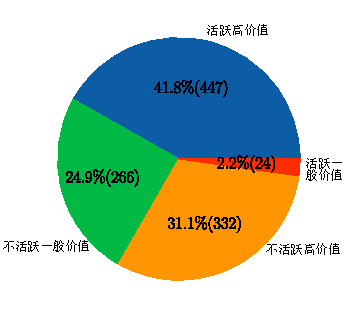
\includegraphics[width=.45\linewidth]{figure/RFM_count_pie.pdf}%
    \label{fig:wellclassbar}}
    \hfil
    \subfloat[RFM维度图]{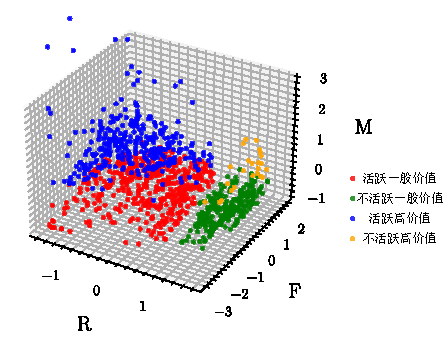
\includegraphics[width=.45\linewidth]{figure/RFM_scatter.pdf}%
    \label{fig:wellclasssca}}
    \caption{气井分类结果}
    \label{fig:classResusca}
\end{figure}
\begin{table}[H]
    \caption{气井分类结果展示表}
    \label{tab:everyclassnumber}
    \begin{tblr}{hlines,vlines,
        columns = {valign=m,co=-1},
        rows    = {halign=c},}
        气井类别 & 数量 \\
        活跃高价值 & 447 \\
        不活跃高价值 & 332 \\
        活跃一般价值 & 24 \\
        不活跃一般价值 & 266 \\
    \end{tblr}
\end{table}

\section{产气量预测实验结果}
\subsection{评估指标}
为了验证本章所提出的基于transformer的气井产量预测算法的有效性,使用两个指标用于评估。其中一个是平均绝对误差(Mean Absolute Error, MAE),其可以衡量
预测值与实际值之间的平均绝对偏差。公式如式\eqref{eq:MAE}所示。
\begin{equation}
    MAE(y, y') = \frac{1}{n} \sum_{i=1}^{n} |y_i - y'_i|
    \label{eq:MAE}
\end{equation}
另一个常用误差指标为累计产量的相对误差,公式如式\eqref{eq:RCPE}所示。
\begin{equation}
    RCPE = \frac{\sum_{i=1}^{n} |y_i| - \sum_{i=1}^{n} |y'_i|}{\sum_{i=1}^{n} |y_i|}
    \label{eq:RCPE}
\end{equation}
上面两式中,$i$表示索引,用于遍历数据集中的每一个数据点。例如,有一个包含多个观测值的数据集,$i$就用来表示这些观测值的序号,从第一个观测值
到第$n$个观测值。$y$表示真实值,也就是实际产量,$\hat{y}$表示预测值,也就是通过模型预测得到的产量。

\subsection{对比实验}
(1)分类预测与不分类预测对比

本次实验将气井分类之后再预测和不分类直接预测进行对比,其对比结果如表\ref{tab:classvalid}所示。为对比是否分类对预测结果的影响,使用本文模型针对未来7天的产气量构建预测模型,分别对每类型井的预测指标和不分类直接进行预测的结果进行统计,使用每类型气井预测结果的中位数作为对
该类预测效果的近似表示。
\begin{table}[H]
    \caption{分类预测与不分类预测结果对比}
    \label{tab:classvalid}
    \begin{tblr}{hlines,vlines,
        columns = {valign=m,co=-1},
        rows    = {halign=c},
        cell{1}{1} = {r=2}{c},
        cell{1}{2} = {c=2}{c},
        cell{1}{4} = {c=2}{c},
        cell{3}{2} = {r=4}{c},
        cell{3}{3} = {r=4}{c}
        }
        气井类别 & 不分类 & & 分类 & \\
          & MAE & RCPE & MAE & RCPE \\
        活跃高价值 & 0.477 & 0.058 & 0.225 & 0.030 \\
        不活跃高价值 & & & 0.367 & 0.051 \\
        活跃一般价值 & & & 0.103 & 0.042  \\
        不活跃一般价值 & & & 0.122 & 0.163  \\
    \end{tblr}
\end{table}
由表中可以看出,在不分类的情况下,预测结果的平均绝对误差(MAE)是0.477,相对百分比误差(RCPE)是0.058。除了不活跃一般价值的RCPE值高于不分类情况下的RCPE以外,这两个值在其他情况下均大于对每一类气井分别进行预测的结果。说明在进行气井产量预测时,先对气井进行分类再进行产气量预测在一定情况下时会达到比较好的效果的。

(2)消融实验

为了验证文中提出的基于Transformer模型中加入时间特征处理层和时域注意力层的有效性,本文对该算法设置消融实验来进行验证。将只加入时间特征处理层、只加入时域注意力层、两者都没有加的模型以及两者都加的模型(本文)在文中数据集上进行训练,
使用其针对未来七天的产气量进行预测,用结果指标的中位值来近视表示其预测结果。本文所得到的实验结果为对所有气井分类后,再按照气井的数量加权得到的。最终结果如表\ref{tab:ablation}所示。
\begin{table}[H]
    \caption{消融实验结果表}
    \label{tab:ablation}
    \begin{tblr}{hlines,vlines,
        columns = {valign=m,co=-1},
        rows    = {halign=c},}
        算法 & MAE & RCPE \\
        两者都无 & 0.736 & 0.377 \\
        仅无时域注意力层 & 0.436 & 0.113 \\
        仅无时间特征处理层 & 0.534 & 0.266 \\
        本文模型 & 0.220 & 0.042 \\
    \end{tblr}
\end{table}
由表中可知,将两个模块都去掉以后,模型的预测结果将显著下降,时间特征处理层对模型准确率的影响大于时域注意力层,这可能是由于气井产气量数据不具备明显的周期性,十分依赖过去的数据导致的。

(3) 对比模型选择

根据前文所述,本问题需要同时对1000余口气井构建时间序列预测模型,且问题包含多种类型的协变量,因此初步选取基于注意力机制的seq2seq模型,lightGBM模型、TFT模型以及本文的模型这四个可以解决这类问题的模型进行实验。

经过对手头的单井日报数据进行处理,累计10年,1000余口气井约有总共约有160多万条数据。为了展示各算法的预测性能,选取数量最多的一类井活跃高价值的产量数据作为测试集进行测试。如表\ref{fig:modelselection}所示,基于注意力机制的seq2seq模型,
由于模型结构限制,无法包含未来时刻的开关井信息,导致预测效果显著劣于其余三个模型。
lightGBM模型、TFT模型及本模型,预测准确率相近,本文算法略优于TFT和lightGBM模型,预测时间本文模型优于TFT和lightGBM模型。但是在模型训练阶段,lightGBM模型(10min)显著快于TFT模型(4h)及本文(1.5h)。故最终保留
本文中的模型和lightGBM模型。
\begin{table}[H]
    \caption{模型选择实验结果}
    \label{fig:modelselection}
    \begin{tblr}{hlines,vlines,
        columns = {valign=m,co=-1},
        rows    = {halign=c},
        cell{2}{1} = {r=4}{c}}
        测试对象 & 模型 & MAE($10^4 \ m^3$) & RCPE(\%)& 预测时间(s)\\ 
        活跃高价值气井& TFT          & 0.241                       & 3.14              & 8.369         \\       
                                    & LightGBM     & 0.334                       & 4.50              & 0.89     \\            
                                    & Seq2seq      & 0.512                       & 10.25             & 5.25   \\             
                                    & Ours         & 0.225                       & 3.02              & 7.29 \\               
    \end{tblr}
    % \centering
    % \begin{tabular}{|c|c|c|c|c|}
    %     \hline
    %     \textbf{测试对象} & \textbf{模型} & \textbf{MAE($10^4 \ m^3$)} & \textbf{RCPE(\%)} & \textbf{预测时间(s)} \\ \hline
    %     \multirow{4}{*}{活跃高价值气井}  & TFT          & 0.241                       & 3.14              & 8.369                \\ \cline{2-5}
    %                                 & LightGBM     & 0.262                       & 3.80              & 0.89                 \\ \cline{2-5}
    %                                 & Seq2seq      & 0.512                       & 10.25             & 5.25                 \\ \cline{2-5}
    %                                 & Ours         & 0.225                       & 3.02              & 7.29                 \\ \hline
    % \end{tabular}
\end{table}
结合图中可以看出,本文的模型在MAE和RCPE指标上的表现均优于其他三种模型,TFT由于参数量太复杂训练和预测时间都较久,效果也稍次于本模型。相对而言,LightGBM模型预测时间较短且也可以取得相对较好的预测结果。
这表明在实时性要求较高的场景中,LightGBM模型可能是一个较好的选择。Seq2seq模型在这三个测试对象上的表现相对较差,可能需要进一步优化模型结构或参数。根据实验结果,可以得出结论:在这三个测试对象上,本模型的预测性能最佳,
但预测时间较长。当实时性要求较高时,可以考虑使用LightGBM模型。

(4)使用部分数据进行预测

本次实验的动机为:由于早期数据缺乏套压记录,这可能会影响预测模型的准确性。近期数据包含了所有重要特征,包括套压数据,并且能够代表整个时间序列的主要趋势和模式,那么只使用近期数据进行预测可能是一个合理的选择。
\begin{table}[h]
    \caption{使用部分数据集训练和使用全数据集训练的对比}
    \label{tab:alldatacomparison}
    \begin{tblr}{hlines,vlines,
        columns = {valign=m,co=-1},
        rows    = {halign=c},
        cell{1}{1} = {r=2}{c},
        cell{1}{2} = {c=2}{},
        cell{1}{4} = {c=2}{},
        }
        气井类别 & MAE& & RCPE & \\ 
        & 使用部分数据 & 使用全部数据 & 使用部分数据 & 使用全部数据 \\ 
        活跃高价值               & 0.193        & 0.225       & 0.023        & 0.030        \\ 
        不活跃高价值               & 0.267        & 0.367        & 0.022        & 0.051        \\ 
        活跃一般价值               & 0.101        & 0.103        & 0.047        & 0.042        \\
        不活跃一般价值               & 0.120        & 0.122        & 0.165        & 0.163        \\ 
    \end{tblr}
\end{table}
为对比预测效果,使用本文模型针对未来7天的产气量构建预测模型,分别使用所有数据和使用2017-01-01之后的数据构建两个不同的模型。根据分类结果将模型划分为四类,使用上文选定的两种模型对这5类型的气井分别进行预测。

    
通过对每类型气井的预测指标进行统计,可以得出以下结论:

对于活跃高价值的气井,使
用2017-01-01之后的数据预测的MAE为0.193,而使用所有数据的MAE为0.225。其RCPE分别为0.028和0.030。这说明基于2017-01-01之后的数据构建的模型预测效果较好。对于不活跃高价值的气井,使用2017-01-01之后的数据预测的MAE为0.267,使用所有数据的MAE为0.367。其RCPE分别为0.022和0.051。这说明对不活跃高价值气井而言,基于2017-01-01之后的数据构建的模型预测效果较好。
对于活跃一般价值的气井,使用2017-01-01之后的数据预测的MAE为0.101,而使用所有数据的MAE为0.103。其RCPE分别为0.047和0.042。对这类气井而言,基于2017-01-01之后的数据构建的模型在MAE上略好,总体来看,这两个模型的预测效果相当。
对于不活跃一般价值的气井,使用2017-01-01之后的数据预测的MAE为0.120,而使用所有数据的MAE为0.122。同时,RCPE分别为0.165和0.163。对于这类气井而言,基于所有数据构建的模型在RCPE上略好,但综合两个指标来看,两个模
型的预测效果相当。

综上所述,在大部分气井类别中,基于2017-01-01之后的数据构建的模型预测效果都较好。

(5)本模型和LightGBM模型对比

实验基本设置: 在这个实验中,本文选用本模型和LightGBM对未来7天的产气量进行预测。实验结果是对属于该日均产气量范围内的所有气井进行预测并计算其指标的中位数统计值得到的。
\begin{table}[H]
    \renewcommand{\arraystretch}{1.5}
    \centering
    \caption{本文模型和LightGBM模型预测结果对比}
    \label{tab:prediction_comparison}
    \begin{tabular}{|c|c|c|c|}
    \hline
    模型     & 气井种类 & MAE & RCPE \\ \hline
    LightGBM & 活跃高价值       &0.334            & 0.072 \\ \hline
    LightGBM & 不活跃高价值     & 0.441           & 0.096    \\ \hline
    LightGBM & 活跃一般价值      & 0.236           & 0.103    \\ \hline
    LightGBM & 不活跃一般价值      & 0.228           & 0.328    \\ \hline
    Ours      & 活跃高价值        &0.225            &0.030      \\ \hline
    Ours      & 不活跃高价值      & 0.367           & 0.051   \\ \hline
    Ours      & 活跃一般价值      & 0.103           & 0.042    \\ \hline
    Ours      &不活跃一般价值      & 0.122           & 0.163    \\ \hline
    \end{tabular}
\end{table}

实验结果对比与分析: 根据上述统计结果表格,可以看出:

从预测性能上看,本文模型在各种情况下都表现出较好的预测性能。然而,从时间角度来看,LightGBM模型的训练和预测时间要远远低于本文模型。具体来说,LightGBM模型的重训练时间为5分钟,而本文模型为半小时;LightGBM模型
的预测时间平均约为1.2秒,而本文模型平均约为7.5秒。这意味着,在实际应用中,使用LightGBM模型会更加节省时间和计算资源。

总结:从实验结果来看,本文模型在预测性能上具有优势,但在时间方面,LightGBM模型具有更好的表现。因此,在实际应用中,企业可以根据实际需求的精度和计算资源进行权衡,选择合适的模型。
\subsection{实验结果统计值展示}
为完整展示实验结果,分别列出两种预测模型分别在预测步长为7天和45天时的预测结果统计指标。
\begin{table}[H]
    \renewcommand{\arraystretch}{1.5}
    \centering
    \caption{本文模型和LightGBM模型预测未来7天内产气量预测结果的MAE指标对比}
    \label{tab:MAE7}
    \begin{tabular}{|c|c|c|c|c|c|c|}
    \hline
    模型     & 气井类别 & MAE mean & MAE std & MAE 25\% & MAE 50\% & MAE 75\% \\ \hline
    LightGBM  &活跃高价值       &0.303     & 0.348   & 0.093    & 0.231     &0.344 \\ \hline 
    LightGBM & 不活跃高价值      & 0.379    & 0.466   & 0.127    & 0.263    & 0.397    \\ \hline
    LightGBM & 活跃一般价值     & 0.280    & 0.279   & 0.099    & 0.236    & 0.311    \\ \hline
    LightGBM & 不活跃一般价值      & 0.299    & 0.369   & 0.095    & 0.228    & 0.377    \\ \hline
    Ours      & 活跃高价值         & 0.189    &0.227    &0.059     & 0.134     &1.239  \\ \hline
    Ours       & 不活跃高价值      & 0.287    & 0.309   & 0.089    & 0.149    & 0.298    \\ \hline
    Ours      & 活跃一般价值     & 0.170    & 0.220   & 0.061    & 0.102    & 0.186    \\ \hline
    Ours     & 不活跃一般价值     & 0.174    & 0.236   & 0.053    & 0.122    & 0.205    \\ \hline
    \end{tabular}
\end{table}
\begin{table}[H]
    \renewcommand{\arraystretch}{1.5}
    \centering
    \caption{本文模型和LightGBM模型预测未来7天内产气量预测结果的RCPE指标对比}
    \label{tab:RCPE7}
    \begin{tabular}{|c|c|c|c|c|c|c|} % Change 'l' to 'c' for center alignment
    \hline
    模型     & 气井类别 & RCPE mean & RCPE std & RCPE 25\% & RCPE 50\% & RCPE 75\% \\ \hline
    LightGBM & 活跃高价值        &0.205     & 0.239     &0.089      &0.153       &0.213 \\ \hline
    LightGBM & 不活跃高价值      & 0.185     & 0.225    & 0.070     & 0.143     & 0.194     \\ \hline
    LightGBM & 活跃一般价值     & 0.231     & 0.247    & 0.068     & 0.193     & 0.267     \\ \hline
    LightGBM & 不活跃一般价值      & 0.533     & 0.945    & 0.097     & 0.228     & 0.577     \\ \hline
    Ours      &活跃高价值         &0.093     & 0.128     &0.022      & 0.031      &0.103 \\ \hline
    Ours      & 不活跃高价值      & 0.086     & 0.119    & 0.015     & 0.035     & 0.080     \\ \hline
    Ours      & 活跃一般价值     & 0.112     & 0.187    & 0.016     & 0.047     & 0.098     \\ \hline
    Ours      & 不活跃一般价值      & 0.363     & 0.757    & 0.066     & 0.163     & 0.358     \\ \hline
    \end{tabular}
\end{table}
统计指标不仅包括中位数,还包括平均数,\%25分位数,75\%分位数,标准差。此处取所有分类结果的均值。其中预测步长7天的MAE结果如表\ref{tab:MAE7}所示。预测步长7天的RCPE结果如表\ref{tab:RCPE7}所示。
预测步长45天的MAE结果如表\ref{tab:MAE45}所示。预测步长45天的RCPE结果如表\ref{tab:RCPE45}所示。
\begin{table}[H]
    \renewcommand{\arraystretch}{1.5}
    \centering
    \caption{本文模型和LightGBM模型预测未来45天内产气量预测结果的MAE指标对比}
    \label{tab:MAE45}
    \begin{tabular}{|c|c|c|c|c|c|c|}
    \hline
    模型       & 气井类别 & MAE mean & MAE std & MAE 25\% & MAE 50\% & MAE 75\% \\ \hline
    LightGBM  & 活跃高价值        & 0.303   & 0.274    &0.098    & 0.278     & 0.398 \\ \hline
    LightGBM  & 不活跃高价值      & 0.460    & 0.429   & 0.151    & 0.353    & 0.518    \\ \hline
    LightGBM  & 活跃一般价值     & 0.345    & 0.291   & 0.108    & 0.286    & 0.406    \\ \hline
    LightGBM  & 不活跃一般价值      & 0.298    & 0.251   & 0.114    & 0.259    & 0.373    \\ \hline
    Ours       & 活跃高价值        &0.153     & 0.188   & 0.069     & 0.128   & 0.233   \\ \hline
    Ours       & 不活跃高价值      & 0.346    & 0.319   & 0.111    & 0.245    & 0.459    \\ \hline
    Ours       & 活跃一般价值     & 0.217    & 0.207   & 0.077    & 0.130    & 0.272    \\ \hline
    Ours       & 不活跃一般价值      & 0.132    & 0.113   & 0.058    & 0.110    & 0.181    \\ \hline
    \end{tabular}
\end{table} 
\begin{table}[H]
    \renewcommand{\arraystretch}{1.5}
    \centering
    \caption{本文模型和LightGBM模型预测未来45天内产气量预测结果的RCPE指标对比}
    \label{tab:RCPE45}
    \begin{tabular}{|c|c|c|c|c|c|c|}
    \hline
    模型       & 气井类别 & RCPE mean & RCPE std & RCPE 25\% & RCPE 50\% & RCPE 75\% \\ \hline
    LightGBM  & 活跃高价值       & 0.185      &0.123    &0.065      &0.151      & 0.204 \\ \hline
    LightGBM  & 不活跃高价值      & 0.191     & 0.207    & 0.069     & 0.156     & 0.214     \\ \hline
    LightGBM  & 活跃一般价值     & 0.217     & 0.221    & 0.087     & 0.174     & 0.260     \\ \hline
    LightGBM  & 不活跃一般价值      & 0.484     & 0.750    & 0.112     & 0.301     & 0.496     \\ \hline
    Ours       &活跃高价值          & 0.073    &0.089      & 0.017     & 0.042     & 0.109 \\ \hline
    Ours       & 不活跃高价值      & 0.087     & 0.094    & 0.019     & 0.047     & 0.120     \\ \hline
    Ours       & 活跃一般价值     & 0.112     & 0.128    & 0.026     & 0.072     & 0.146     \\ \hline
    Ours       & 不活跃一般价值      & 0.361     & 0.431    & 0.071     & 0.146     & 0.319     \\ \hline
    \end{tabular}
\end{table}
% 
\begin{figure}[H]
    \centering
    \subfloat[井XE8867-HU预测结果]{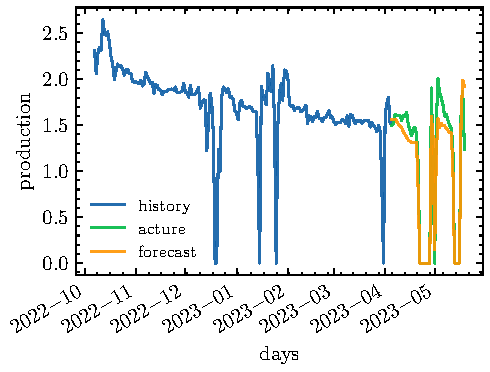
\includegraphics[width=.45\linewidth]{figure/forecast_SN0018-03.pdf}}
    \hfil
    \subfloat[井XE3878-RE预测结果]{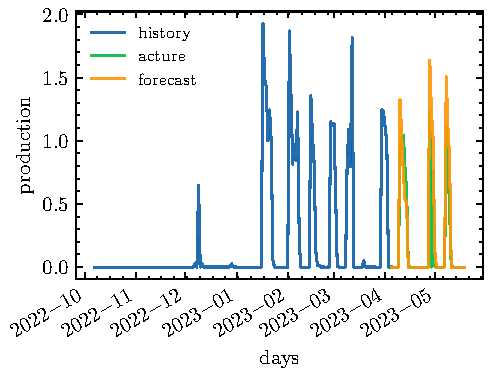
\includegraphics[width=.45\linewidth]{figure/forecast_SN0037-01.pdf}}
    \caption{气井预测结果展示(第一部分)}
    \label{fig:6predicre_part1}
\end{figure}

\begin{figure}[H]
    \ContinuedFloat
    \centering
    \subfloat[井LR7359-BR预测结果]{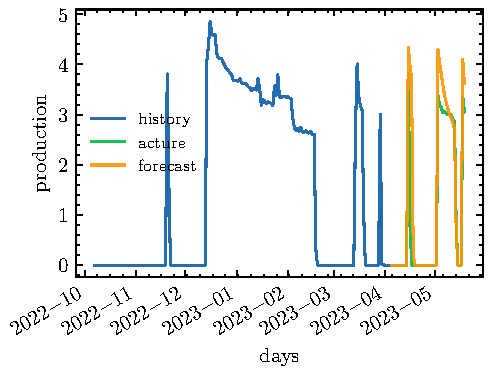
\includegraphics[width=.45\linewidth]{figure/forecast_SN0087-03i.pdf}}
    \hfil
    \subfloat[井RC8375-BN预测结果]{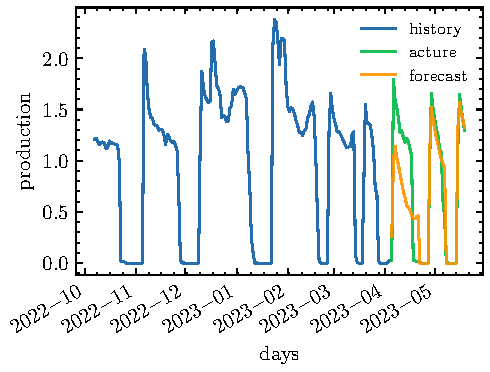
\includegraphics[width=.45\linewidth]{figure/forecast_SN0095-06.pdf}}
    \hfil
    \subfloat[井SI2938-KI预测结果]{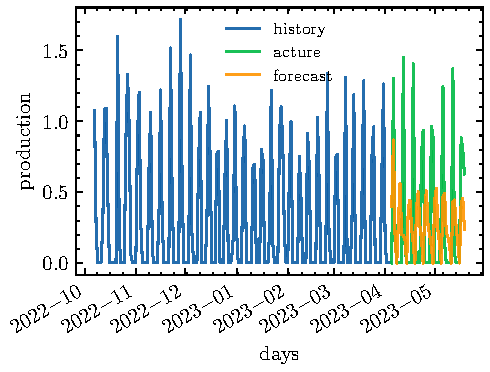
\includegraphics[width=.45\linewidth]{figure/forecast_SN0049-08.pdf}}
    \hfil
    \subfloat[井SI2938-KI预测结果]{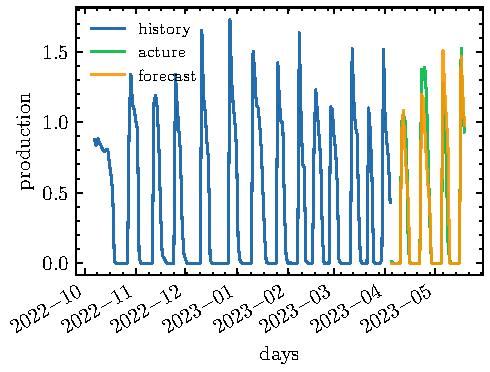
\includegraphics[width=.45\linewidth]{figure/forecast_SN0075-04ST.pdf}}
    \caption{气井预测结果展示(第二部分)}
    \label{fig:6predicre_part2}
\end{figure}
为直观展示预测结果,选择6口气井的预测结果如\ref{fig:6predicre_part2}所示。
\section{开关井推荐}
本小节将应用产气量预测的结果,根据企业日常开关井的规则进行开关井的策略推荐。
\subsection{算法设计}
气井开采过程中,通常会产生一定量的液体,包括水和油。产液量的增加会影响气井的产气量,因为液体在井筒中的积累会增加井筒的阻力,使气流的速度降低,
从而影响气井的产气量。当气井处于低压低产阶段时,气相不能有效地携带液体,会导致积液现象。此时,如采用间歇生产方式(即周期性地开关井),可以利用
关闭期间积累的压力差,在开启时将积聚在底部或中部的液体迅速排出。

但如果开关频率过高或关闭时间过短,则可能造成反复积排液、增加摩阻损失、降低生产效率。可若是开关频率过低或关闭时间过长,则可能导致底部水锥突
破、增加水含率、降低天然气质量。
\begin{algorithm}[H]
    \baselineskip=20pt
    \caption{开关井策略}
    \label{al:openclose}
    \begin{algorithmic}[1]
    \Require $df$: Dataset, $all\_forecasts$: 未来7天的预测结果, $auto\_well$: 自动切换井号, $target$: 目标值, $well\_no\_disable$: 不投入生产的井, $threshold$: 停产门槛, $pressure\_threshold$: 压力门槛,
    \Ensure $close\_wells$: 需要关闭的井列表, $open\_wells$: 需要开启的井列表, $close2open\_wells$: 从关闭状态切换到开启状态的井列表, $open2close\_wells$: 从开启状态切换到关闭状态的井列表
    
    \State 初始化 $close\_wells$, $open\_wells$, $close2open\_wells$, $open2close\_wells$
    \State 获取当前日期为 $dates\_time$
    \State 确定因压差过大需要临时关闭的井为 $need\_close\_by\_pressure$
    \State 获取当前开启和关闭井的信息为 $df\_open\_0$, $df\_close\_0$
    
    \For{$i = 1$ \textbf{至} $7$}
        \State 确定尚未达到开启时间的井为 $still\_need\_close\_no$
        \State 确定产量低于门槛需要关闭的井为 $need\_close\_by\_threshold$
        \State 确定在第$i$天需要关闭的井为 $need\_close\_no_i$ 
        \State 确定在第$i$天仍然可以开启的井为 $still\_can\_open\_no_i$ 
        \State 确定在第$i$天可以从关闭状态切换到开启状态的井为 $can\_close2open\_no_i$ 
        \State 确定在第$i$天可以从开启状态切换到关闭状态的井为 $can\_open2close\_no_i$ 
        \State 计算第$i$天的当前产量为 $cur\_production_i$
        \State 计算关闭井后的产量差值为 $delta_i$ 
        \If{$delta_i > 0$}
            \State 依次关闭开启时间较长的井来更新 $open2close\_wells_i$
        \Else
            \State 依次选择开启产量较高的井来更新 $close2open\_wells_i$
        \EndIf
        
        \State 更新第$i$天关闭的井列表为 $df\_close_i$
        \State 更新第$i$天开启的井列表为 $df\_open_i$
    \EndFor
    
    \State \Return $close\_wells$, $open\_wells$, $close2open\_wells$, $open2close\_wells$
    
    \end{algorithmic}
  \end{algorithm}

在此背景之下,本节基于第\ref{cha:data}节提供的数据,并借鉴专家经验,对开关井策略提出了建议。具体的推荐流程如算法\ref{al:openclose}所述。首先,进行产气量的预测,以估算第i天的产气量。然后,以企业设定的目标产气量$target$、不参与投入生产的井列表$well\_no\_disable$、根据经验规则自动进行开关控制的井列表$auto\_well$、以及设定的停产和压力门槛值$threshold$和$pressure\_threshold$为依据,进行开关井策略的制定。

策略制定的具体步骤包括:首先,排除因当日压力差异过大而暂时关闭的井,这些井在关闭后通常需要较长的时间进行调整。接着,获取当前的开关井状态信息。对于未来的第i天,需要排除那些根据企业规定尚未达到开井时间的井,并根据设定的停产门槛识别出产量低于阈值且需要关闭的井。

随后,综合考虑达到停产门槛、压力门槛的井、不投入生产的井以及企业规定第i天需保持关闭状态的井,来确定第i天所有需要关闭的井。其次,从已经关闭的井中,除了那些已经标记为不再投入生产的井之外,识别出尚未达到停产门槛和压力门槛的井,这些井是可以被重新开启的。

最后,计算当前产量,并在可开启和可关闭的井中进行选择,执行开关井操作。通过比较操作前后的产量差值,如果差值大于零,则应进一步关闭开启时间较长的井;如果差值小于零,则应优先开启产量较高的井。通过这一流程,最终确定开关井的结果。

\subsection{结果展示}
选取目标产气量为1000($10^4m^3$),压力阈值为2.0($MPa$),最终的得到的开关井推荐结果如图\ref{fig:openclosereco}所示。更详细的开井关井的具体信息将在第六章系统实现中展示。
\begin{figure}[H]
    \centering
    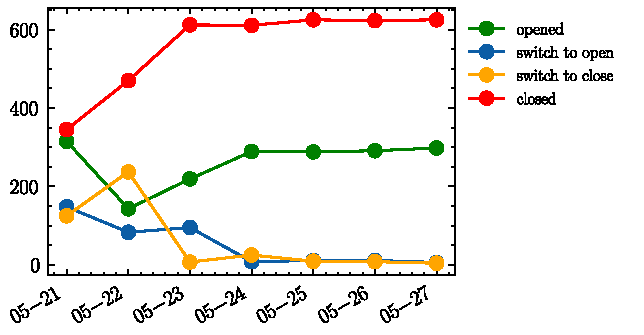
\includegraphics[width=.8\linewidth]{figure/reco.pdf}
    \caption{开关井推荐结果}
    \label{fig:openclosereco}
\end{figure}

  \section{本章小节}
  本章对前文提出的气井分类算法和气井产气量预测算法的结果进行了展示。气井被分为四类,通过对比实验发现,先分类再进行预测的准确率高于直接对气井进行预测的准确率。并通过消融实验证明了第四章基于Transformer的产气量预测算法模块的有效性。通过对实验结果树枝对比,发现GRU对模型准确性的
  影响大于Transformer。随后,本文通过实验选取了LightGBM作为本文算法的对比算法,经过实验得出本文算法在预测准确率上高于LightGBM算法,但在预测时间上慢于LightGBM算法,因此保留两种模型以供企业在需要进行产气量预测时根据不同的需要挑选模型。最后,本文应用了对产气量预测后的预测结果,
  根据企业的专家知识结合预测结果提出了开关井策略推荐算法,展示了算法流程,以及最后的推荐结果。
\chapter{系统设计与实现}
本章根据企业的的痛点需求,设计并实现了一个气井智能管控系统,系统包含了第三章的
结合RFM与核密度估计的气井分类算法和第四章的基于transformer的气井产量预测算法及开关井推荐算法。
主要功能有数据连接,数据管理和智能分析等模块。
\section{系统需求分析}
\subsection{总体需求分析}
某油田企业作为行业的重要参与者,面临着诸多数字化建设方面的挑战。随着气井数量的增多以及老井的管理难度加大,需要按照气井全生命周期管理理念,引入机器学习、大数据分析等前沿技术,提升气井生产管理的研究决策质量和效率。其在数字化建设中主要遇到下列问题:

首先,过去企业缺乏对数据的智能分析,主要依赖于传统的、基于经验的决策方式,这种做法未能充分利用现有数据资源,从而导致生产计划不稳定、资源利用效率低下等一系列问题。此外,尽管企业过去积累了大量的数据,但由于缺乏有效的智能分析工具,这些宝贵的数据资源并未被充分利用,造成了资源的极大浪费。

其次,随着智能分析需求的不断深入,需要引入地质、钻探、环境等数据等时,该企业发现其所涉及的气井数据呈现出高度的多样性和复杂性。地质数据和钻探数据的来源及格式多样,加之企业内部是按职能划分的垂直部门结构,导致不同部门间存在较大的生产数据格式差异。同时,企业在软
件应用上高度分散,各业务单元采用
不同的软件系统存储数据,这极大地增加了在智能分析过程中进行数据处理的难度。

针对以上问题,该企业迫切需要建立一个软件结构合理的气井管控系统。该系统应能够对气井数据进行智能分析,利用机器学习的方式科学地指导未来决策。
同时可以有效地整合、存储和管理各类数据,包括来自不同软件和不同格式的数据。
通过建立这样一个系统,该油田企业能够通过数据的高效共享与分析,来为企业的决策提供科学依据和参考。

本系统面向的是油田企业的员工,他们的计算机基础较为薄弱,期望使用简单易懂的界面,通过简单的操作加载数据并获取所需结果。具体包含了以下需求:

(1)拥有智能分析功能:可以对数据进行智能分析。系统可以对气井数据进行分类、产气量预测和开关井推荐,提升气井及生产管理的研究决策质量和效率。

(2)可以对多元异构数据对接和导入:可以从不同来源采集数据并统一存储在数据湖中,保留原始数据信息。可以处理来自不同系统、不同格式的数据,可以进一步的智能分析提供更加全面的数据资源。

(3)具有数据管理的功能:可以对导入到数据湖的数据进行持久化保存。此外,系统支持数据集定时和周期任务的调用,使数据处理过程更加自动化和高效。

通过对系统进行总体的需求分析,对气井智能管控系统进行模块划分。
具体包括以下三个模块:数据连接、数据管理和智能分析。其模块划分图
如图\ref{fig:allmodules}所示。
\begin{figure}[H]
    \centering
    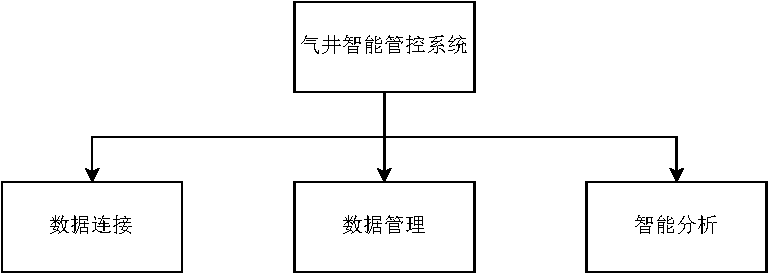
\includegraphics[width=.5\linewidth]{figure/systemincludemodles.pdf}
    \label{fig:allmodules}
    \caption{气井智能管控系统模块划分图}
\end{figure}
\subsection{系统功能性需求}
(1)智能分析

智能分析是系统最重要的部分,目前的模块包括第二章和第三章的气井分类、产气量预测和开关井推荐操作。其中产气量预测可以让用户选择气井号,选择预测步长和开始预测日期,同时还提供模型效果检验功能。开关井推荐可以根据用户想要达到的产量目标、压力差阈值和用户想要
排除的不参与生产的井来进行开关井的推荐。
\begin{figure}[H]
    \centering
    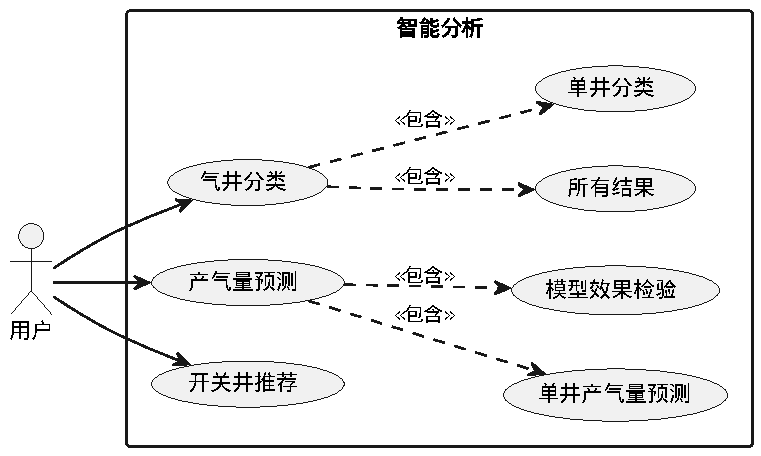
\includegraphics[width=.7\linewidth]{figure/智能分析用例图.pdf}
    \caption{智能分析用例图}
    \label{fig:analyusecase}
\end{figure}

(2)数据连接

在气井智能管理系统中,数据连接模块负责从多种数据源中采集和导入数据。油田企业的数据通常存储在关系型数据库(如MySQL、SQL Server)中,也可能以CSV文件的形式存储。此外,油田数据还涉及到非关系型数据库(如HBase)和流式消息中间件(如Kafka)等数据源。
数据连接管理模块设计具有良好的扩展性,能够根据需要灵活添加新的数据源。在油田数据连接管理中,用户首先选择目标数据源,然后创建相应类型的数据连接,并填写相关的连接信息,如数据库地址、用户名、密码等。完成连接信息后,用户可以将连接信息持久化保存,以便后续使用。
其用例图如图\ref{fig:dataconnectionusecase}所示。
\begin{figure}[H]
    \centering
    \label{fig:dataconnectionusecase}
    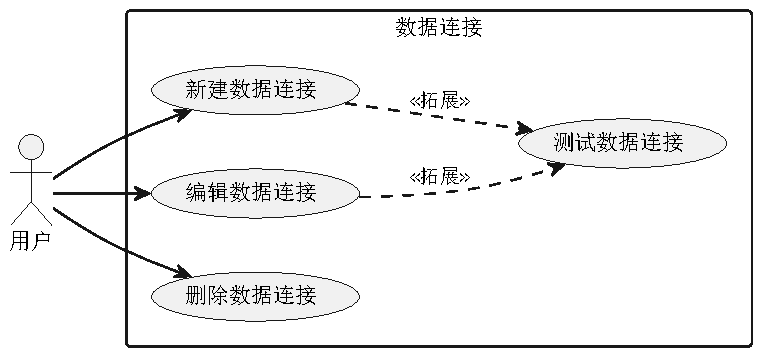
\includegraphics[width=.7\linewidth]{figure/数据连接用例图.pdf}
    \caption{数据连接用例图}
\end{figure}

(2)数据管理 

数据管理包括对数据集进行目录管理、数据集管理以及对数据集更新。其中数据集管理包括新建数据集、浏览数据集等。
\begin{figure}[h]
    \centering
    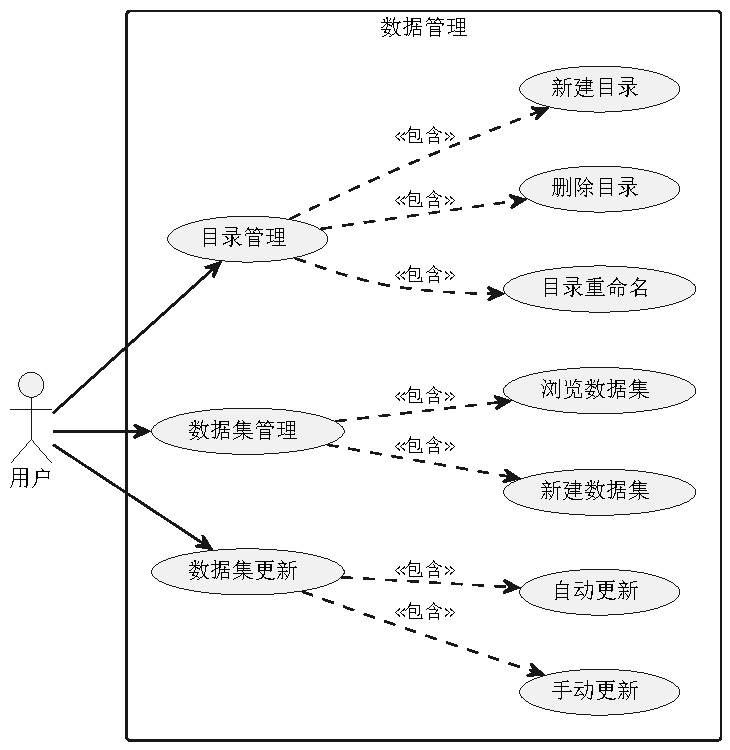
\includegraphics[width=.6\linewidth]{figure/数据管理用例图 .pdf}
    \caption{数据管理用例图}
    \label{fig:datamaucase}
\end{figure}
新建数据集可以通过数据库数据集,SQL数据集,文件数据集,上传文件等方式创建。其中数据库数据集是直接从已有的数据连接中选择的数据库中的表作为数据集。
SQL数据集可以通过SQL语句和从已有的数据连接中获取返回结果作为数据集。
文件数据集表示用户导入本地Excel文件,上传为数据集。数据集更新主要包括对数据集手动更新或者通过定时/周期任务来更新。
上传文件表示用户导入本地其他类型的文件,上传为数据集。目录管理可以查看数据的各种结构关系。具体如\ref{fig:datamaucase}所示。

上文中对系统进行了总体需求分析和功能需求分析,但除了对必要的功能进行需求分析之外,气井智能管控系统还需要在响应时间、易用性等非功能的需求方面保障用户的使用体验。

(1)响应时间

在实际开发中,一般要求系统处理请求并返回结果的总耗时在一定时间内。对于系统的响应时间,通常会要求在3000毫秒内完成。此处要求一般任务可以在500ms内完成。
本项目最耗时的部分为数据导入、更新和智能分析部分。此处要求单个数据集的导入时间不超过0.5h,并可允许同时有5个气井数据进行导入/更新;智能分析模块中,气井预测可能耗时相对较久,此处要求气井预测时间不超过10s,

(3)易用性

系统的易用性是指用户在使用系统时的感受和体验,主要体现在用户能够轻松地学习、理解、操作系统,以及完成任务的效率和满意度。企业员工大多数计算机基础薄弱,因此系统提供了简洁明了的前端界面让用户进行数据管理和数据分析操作,可以让他们在不了解数据库、算法的前提下也能较快进行自己想要的操作。
同时提供了友好的反馈机制,能够及时给予用户反馈,包括操作结果、错误提示、进度指示等,让用户清楚地了解当前状态和下一步行动。
\section{系统总体设计}
根据前文的系统需求分析,系统主要分为三个模块:智能分析、数据连接和数据管理。

为了描述清楚系统内部各模块和组件之间的相互关系,此处将系统分为多个层次,通过系统架构图的方式,图形化地展示系统的实现模式
和工作模式。具体如图\ref{fig:sysstruc}所示。

由图中可以看出,系统采用分层的架构设计,这些层相对独立,各自专注于实现自身的功能,而不会直接依赖于其他层次的实现细节。层与层之间通过暴露的接口进行交互,实现数据和控制流的传递。有助于降低系统内部的耦合度,即各个组件之间的依赖关系较弱,提高了系统的灵活性和可维护性。
系统由底向上主要分为数据接入层,数据存储层、业务层和可视化层。下面是各个层的详细介绍。
\begin{figure}[H]
    \centering
    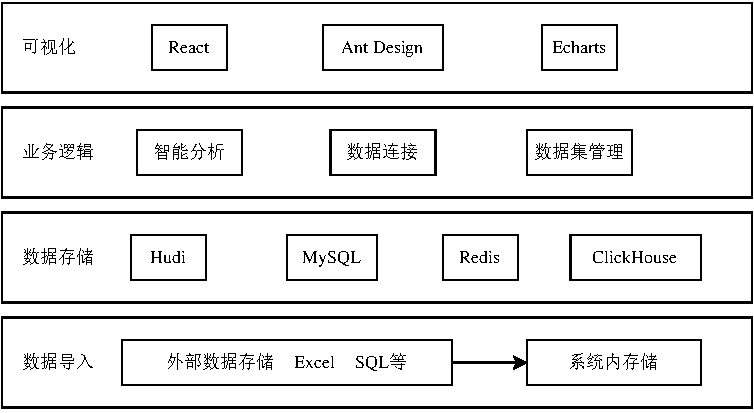
\includegraphics[width=.9\linewidth]{figure/系统架构图.pdf}
    \caption{气井智能管控系统架构图}
    \label{fig:sysstruc}
\end{figure}
(1)数据接入层

数据接入层负责将外部的异构数据导入到系统中,其中外部的异构数据源包括数据库数据(关系型数据库如SQL Server、MySQL;非关系型数据库HBase;外部文件数据CSV、XML、JSON等)。这些数据将通过Spark来导入到数据湖Apache Hudi中。
Spark提供了多种接口来对应不同的文件类型数据的导入。

(2)数据存储层

数据存储层主要是对系统中所有数据进行持久化的存储。其中包括大数据存储、业务数据存储和数据缓存。其中大数据存储主要通过数据湖框架Apache Hudi来对原始数据进行持久化存储,前面数据接入层的多源异构数据主要存储在这里。
业务数据主要存储在MySQL中,业务数据主要是针对系统提供服务,保证系统的正常运行。Redis和ClickHouse主要负责数据的缓存,其中Redis缓存的是业务数据,例如用户会话信息、登录状态、用户配置等。clickHouse主要是用于数据分析
过程,进行数据计算和中间结果的存储。

(3)业务层 

业务层负责处理业务逻辑和功能实现。它包含了系统的核心功能模块,通过提供访问接口来解析用户的行为,并将其转化为系统内部的各种调用。在业务层中,不同的功能模块专注于各自的业务规则和业务对象之间的交互,执行完毕后将结果返回给可视化层。
业务层采用高内聚、低耦合的系统设计思路,确保各个功能模块之间的独立性和可维护性,同时按照对扩展开放的原则进行设计,以保证整体业务的可扩展性。
业务层具体包含了数据连接、数据管理、智能分析、可视化展示和用户权限几个模块。

(4)可视化层

可视化层是用户与系统的桥梁,用户通过在前端进行操作来完成自己的一系列业务需求。系统使用React作为可视化框架,采用Ant Design作为前端的UI组件库,使用Echarts来创建丰富、交互式的数据可视化图表,并通过Axios和WebSocket来
实现钱后端的通信。

\section{系统业务模块设计与实现}
本节根据前文中提出的系统的业务模块,通过对重要的数据连接、数据管理和智能分析模块的实现类图进行详细的描述,介绍系统业务模块的设计。
\subsection{数据连接模块}
数据连接用于将目标数据源连接到系统中,接入系统中的目标数据源可以在后续的进行数据管理、数据分析等一系列操作。数据连接类型的类图如图\ref{fig:dataconneclass}所示。
\begin{figure}[H]
    \centering
    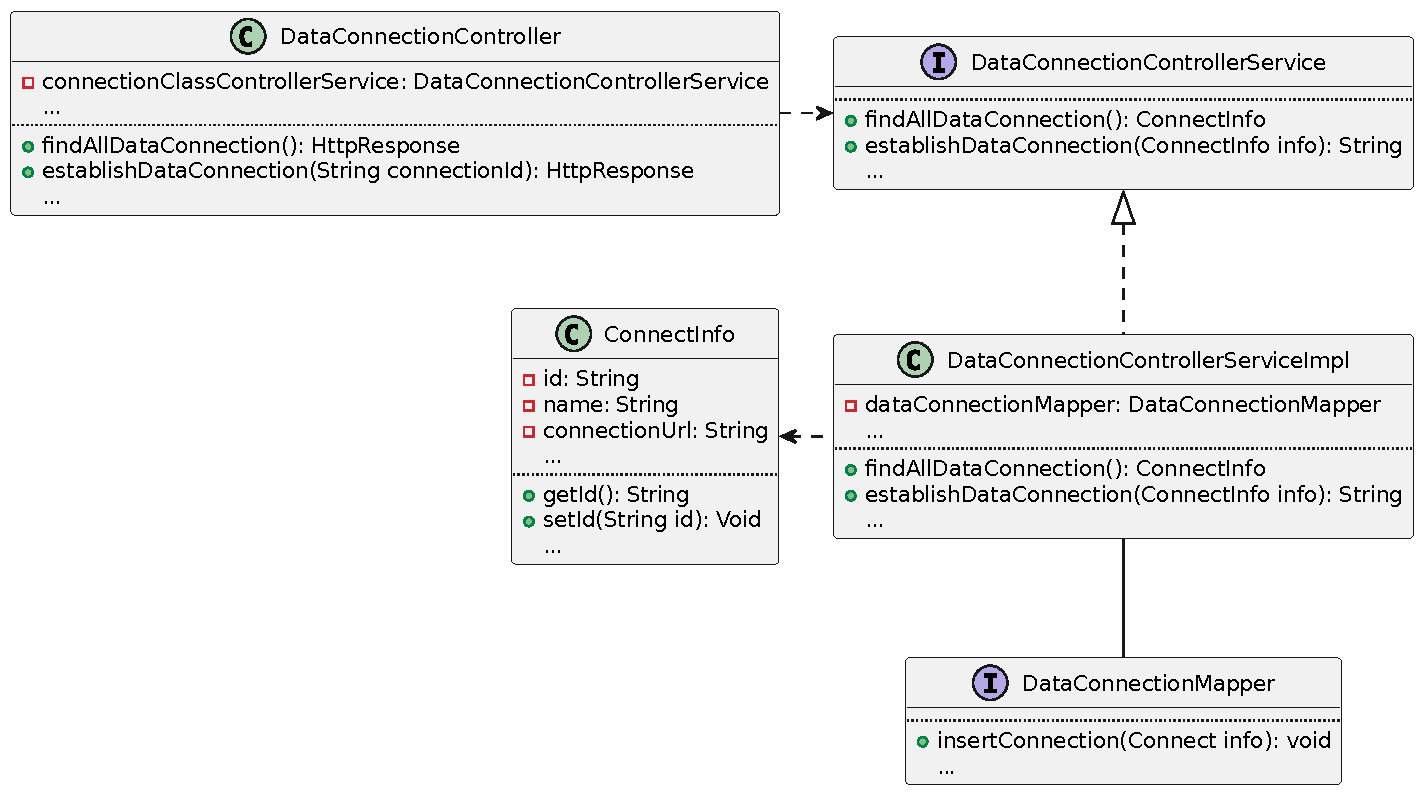
\includegraphics[width=.9\linewidth]{figure/数据连接类图.pdf}
    \caption{数据连接类图}
    \label{fig:dataconneclass}
\end{figure}
当系统用户发起一个请求时,DataConnectionController负责接收这个请求并解
析其中的参数。它随后会调用DataConnectionControllerService中定义的方法来执行具体的操作。DataConnectionControllerServiceImpl类实现了DataConnectionControllerService接口,它包含了系统
的主要业务逻辑。用户访问数据连接页面时,系统会调用 findAllDataConnection()
方法来检索系统中所有已建立的数据连接实例。在这个页面上,用户可以通过执行
establishInstance() 方法来创建一个新的数据连接实例,通过执行 testConnection() 方法
来测试现有数据连接是否正常工作,通过调用 deleteDataConnection() 方法来删除
一个数据连接实例,通过调用 modifyDataConnection() 方法来更新数据连接的信
息,以及通过调用 findDataConnectionInfo() 方法来查看已存在的数据连接配置信
息。DataDataConnection类是数据连接
实例的实体类,存储了平台中数据连接实例的信息,包括连接名称、连接 URL、连接
实例信息(用户名、密码等)等。DataDataConnectionMapper是用于与
数据库中数据连接实例信息表交互的接口。
\subsection{数据管理模块}
数据管理模块主要包括三个部分:目录管理、数据集管理和数据集更新。在目录管理中,主要任务是整理数据集的存储位置,确保它们正确归档在特定文件夹内。目录由不同的节点组成,包括文件夹和数据集本身,它们在目录中以不同的方式标记以便区分。保持这些节点之间的层次结构有助于形成一个有层次的目录结构。
在数据集管理方面,可以创建、删除、复制和查看数据集,以便有效地管理它们。

对于数据集更新,它允许数据集按计划或周期性地更新。更新可以是自动的,也可以是手动的。每个数据集都有一个关于如何更新的设置,如果用户未做设置,则使用默认配置。根据这些设置,平台会定期或按需更新数据集,并记录更新任务的详细信息和状态。
更新时,系统确保每个数据集同时只能有一个更新任务在进行。这是通过检查一个特殊的Map实现的,该Map确保每个数据集同时只有一个关联的更新任务正在运行。更新任务的执行是多线程的,使用了一个特定的线程池,该线程池可以调度周期性任务。对于一次性的手动更新,任务会直接提交给线程池执行。
数据管理模块的类图如图\ref{fig:datamanageclass}所示。

当前端发出请求时,DataManagementController将充当主要接口来处理并分析这些请求。目录和数据集的管理任务都通过DataSourceService接口完成,而数据集的具体动作则是由DatasetUpdateServiceImpl接口负责。在这种设置下,文件夹和数据集被看作是目录结构的元素,它们虽然共处一个层级,但通过不同的方式标记以区分。
在实现方面,DirectoryServiceImpl和DatasetImpl分别实现了DataSourceService接口的具体职责,处理不同的数据管理需求。当用户进入数据管理页面时,系统首先会调用getTotalCatalog()方法来获得全部资源目录结构。通过makeRootDir()方法可以创建在根目录创建新的文件夹,此外,还可以对文件夹进行移动、删除、重命名等操作。
通过文件夹进入到具体的数据集后,DatasetImpl的previewData()方法会将得到数据集的具体内容,前端通过与controller通信读取内容后经过处理,可以将预览数据集的结果显示在用户界面上。该处还支持用户通过establishDIYDataset()等方法上传自己的数据集、Excel文件、删除数据集等。
在数据模型方面,本文区分了两种类型的信息实体:DirectoryInfo 代表目录节点,而 DatasetInfo 代表数据集节点。DatasetUpdateServiceImpl是对DatasetUpdateService接口的实现,当进入数据集的更新设置页面后,会先调用getDatasetUpdateInfo()方法来查看
数据集已有的更新设置。随后可以通过setDatasetUpdateInfo()或setAllDatasetUpdateInfo()来修改一个或多个数据集的更新设置。修改完更新设置后,可以通过startDatasetUpdateTask()方法来启动一个更新任务,目前系统近支持
全量更新。随后可以关闭更新任务。同时getAllDatasetUpdateInfo()方法也可以查看用户的所有数据集更新信息。
\begin{figure}[H]
    \centering
    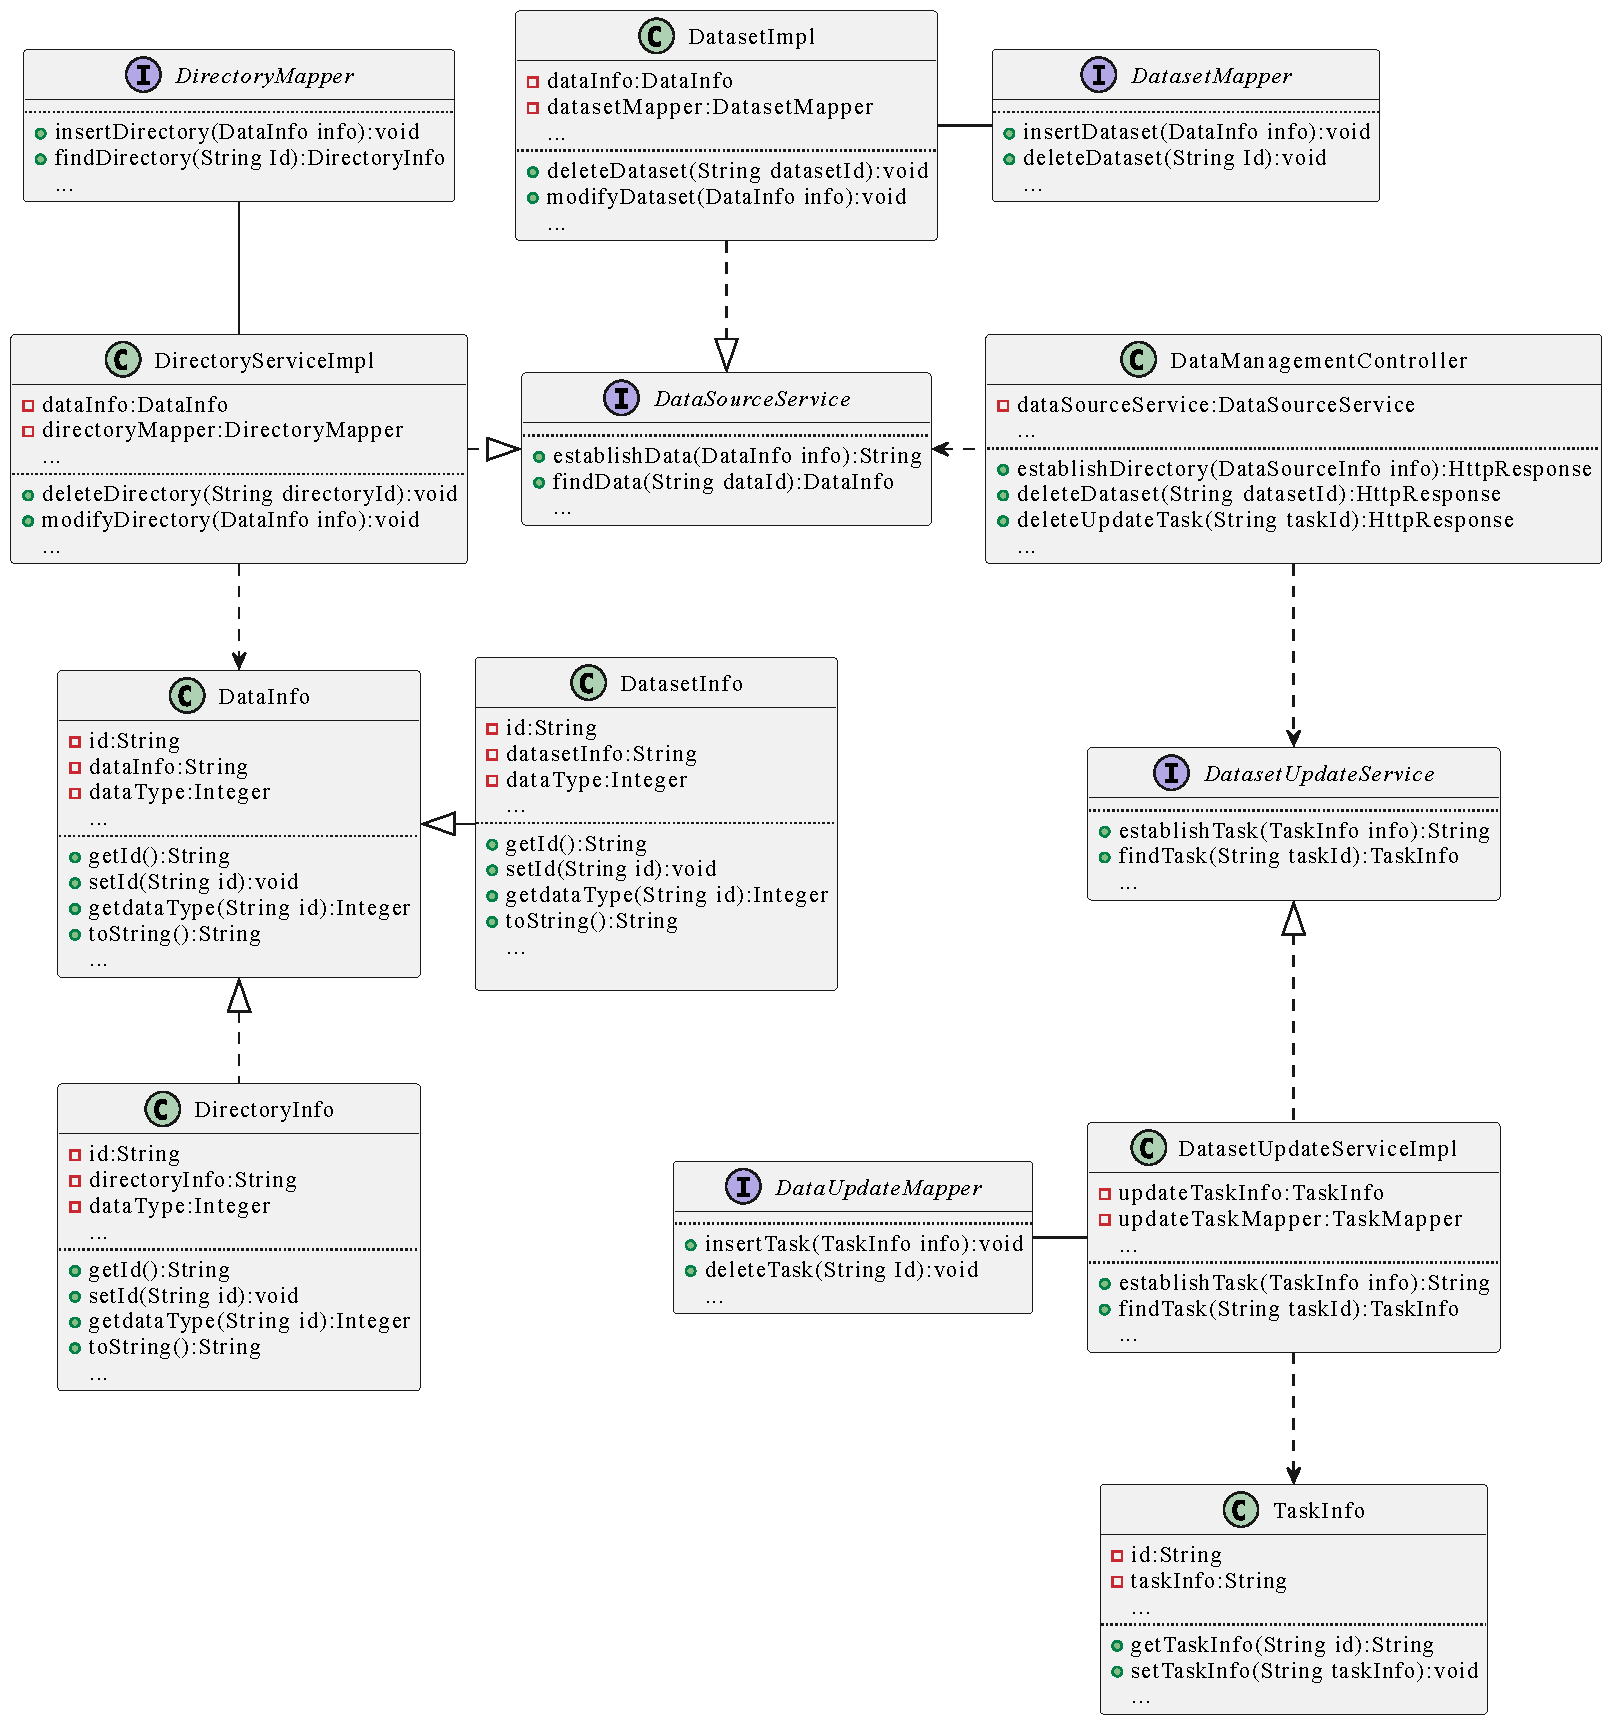
\includegraphics[width=.9\linewidth]{figure/数据管理类图.pdf}
    \caption{数据管理类图}
    \label{fig:datamanageclass}
\end{figure}
最后,为了实现数据的持久化,系统设计了三个映射类:DirectoryMapper、DatasetMapper 和 DatasetUpdateMapper,它们分别对应于目录管理、数据集管理和数据操作功能,确保所有相关数据都能被持久化存储并管理。
系统的架构遵循Controller-Service-Mapper-Model模式,以上提及的各个类相互配合,一起完成数据连接模块的全部功能。
\subsection{智能分析模块}
智能分析模块主要包括气井分类、产气量预测、开关井推荐。其中气井分类为第三章通过时间序列聚类对气井聚类之后的结果,用于企业对气井的精细化管理。产气量预测为第四章产气量预测的结果,企业可以根据预测结果完成进行
策略制定。开关井推荐也在第四章做过介绍,企业可以根据开关井推荐的结果来进行相应的开关井操作。
智能分析模块的类图如图\ref{fig:analyclass}所示。
\begin{figure}[H]
    \centering
    \includegraphics[width=.9\linewidth]{figure/智能分析类图.pdf}
    \caption{智能分析类图}
    \label{fig:analyclass}
\end{figure}
由于智能分析多是用Python进行算法实现,具体实现算法已经在前文进行了介绍。因此当前端进入智能分析页面后,IntelligentAnalysisController接口会分析findAllCluster()的参数,然后在IntelligentAnalysisServiceImpl类中调用Python结果,通过WellMapper查询气井信息,最后将结果展示在首页。
产气量预测与开关井推荐等也类似该方法。
\section{系统测试}
\subsection{测试环境说明}
气井智能管控系统的测试环境分为硬件环境和软件环境,表\ref{tab:systesthaen}所示为气井智能管控系统的硬件测试环境。其中硬件环境包括数据库服务器、业务服务器和Hudi集群。

数据库服务器包括存储业务数据的MySQL及业务数据的缓存ClickHouse。业务服务器主要包括钱后端以及Python的部署,可以用来执行操作逻辑处理业务需求。Hudi集群采用三节点配置,包括一个主节点和两个从节点,此分布式设置增强了数据持久化存储的稳定性与安全性。
\begin{table}
    \caption{硬件测试环境信息}
    \label{tab:systesthaen}
    \begin{tblr}{hlines,vlines,
        columns = {valign=m,co=-1},
        rows    = {halign=c},
        cell{3}{1} = {r=3}{c}
        }
        服务器类型 & CPU& 内存 & 磁盘 & 操作系统 \\ 
        数据库服务器    & Intel(R) Xeon(R) CPU E5-2683 v3 & 16G       & 500G      & Centos7    \\ 
        Hudi集群 & Intel(R) Xeon(R) CPU E5-2683 v3 & 8G        & 2TB       & Centos7   \\ 
        & Intel(R) Xeon(R) CPU E5-2683 v3 & 4G        & 1TB       & Centos7  \\
        & Intel(R) Xeon(R) CPU E5-2683 v3 & 4G        & 1TB       & Centos7  \\ 
        业务服务器      & Intel(R) Xeon(R) CPU E5-2683 v3 & 8G        & 500G      & Centos7   \\ 
    \end{tblr}
    % \begin{tabular}{|l|c|c|c|c|} % CPU列水平和垂直居中
    %     \hline
    %     \textbf{服务器类型} & \textbf{CPU}& \textbf{内存} & \textbf{磁盘} & \textbf{操作系统} \\ 
    %     \hline
    %     数据库服务器    & Intel(R) Xeon(R) CPU E5-2683 v3 & 16G       & 500G      & Centos7    \\ 
    %     \hline
    %     \multirow{3}{*}{Hudi集群} & Intel(R) Xeon(R) CPU E5-2683 v3 & 8G        & 2TB       & Centos7   \\ 
    %     \cline{2-5} & Intel(R) Xeon(R) CPU E5-2683 v3 & 4G        & 1TB       & Centos7  \\
    %     \cline{2-5} & Intel(R) Xeon(R) CPU E5-2683 v3 & 4G        & 1TB       & Centos7  \\ 
    %     \hline
    %     业务服务器      & Intel(R) Xeon(R) CPU E5-2683 v3 & 8G        & 500G      & Centos7   \\ 
    %     \hline
    % \end{tabular}
\end{table}
表\ref{tab:systestsoen}
所示为气井智能管控系统的软件测试环境。
\begin{table}
    \caption{软件测试环境信息}
    \label{tab:systestsoen}
    \begin{tblr}{width = \textwidth,
        colspec = {|X[c]|X[c]|X[c]|X[c]|},
        hlines, vlines,
        columns = {valign=m},
        cell{4}{1} = {r=4}{c} }
        模块名称 & 软件名称 & 版本号 \\ 
        Java开发 & JDK &1.5 \\
        算法开发 & Python & 3.9 \\
        数据存储 & MySQL & 5.6 \\
        & Redis &4.0 \\
         & ClickHouse & 21.10 \\
         & Hudi & 0.11.0 \\
    \end{tblr}
\end{table}
\subsection{系统功能性测试}
本小节从系统功能性需求出发,为每个模块设计测试用例和场景并记录结果。

(1)数据连接

数据连接管理模块主要包括新建数据连接、删除数据连接、编辑数据连接和测试
连接四个功能,其测试用例如表\ref{tab:testcon}所示。
\begin{table}[H]
    \caption{数据连接测试用例}
    \label{tab:testcon}
    \begin{tblr}
    {
    hlines,vlines,
    columns = {valign=m,co=-1},
    rows    = {halign=c},
    row{1}  = {font=\bfseries\boldmath},
    }
    编号 & 用例说明     & 测试步骤                                               & 预期结果                             \\
    1    & 创建数据连接 & {选择新建数据连接,输入数据库\\配置参数,完成数据连接} & 新建数据连接成功                     \\
    2    & 删除数据连接 & 选择一个数据连接,点击删除按钮                         & 删除数据连接成功                     \\
    3    & 编辑数据连接 & 选择一个数据连接,修改其参数配置并提交                 & 编辑数据连接成功                     \\
    4    & 测试数据连接 & 选择一个数据连接,选择测试按钮                         & {测试这个数据连接\\当前是否是成功的} \\
    \end{tblr}
\end{table}

根据表\ref{tab:testcon}的测试内容,可以在数据连接页面进行创建、删除、编辑和测试连接等操作。图\ref{fig:login}为系统的登陆界面。图\ref{fig:dataconre}为数据连接的界面。

\begin{figure}[H]
    \centering
    \includegraphics[width=.99\linewidth]{figure/login.pdf}
    \caption{气井智能管控系统登陆界面}
    \label{fig:login}
\end{figure}
\begin{figure}[H]
    \centering
    \includegraphics[width=.99\linewidth]{figure/数据连接.pdf}
    \caption{数据连接界面}
    \label{fig:dataconre}
\end{figure}

(2) 数据管理

由前文可知数据管理分为目录管理、数据集管理和数据集更新。其中目录管理测试用例如表\ref{tab:direte}所示。
\begin{table}[H]
    \caption{目录管理测试用例}
    \label{tab:direte}
    \begin{tblr}{hlines, vlines,
        columns = {valign=m,co=-1},
        rows    = {halign=c},
        row{1}  = {font=\bfseries\boldmath},
        }
        编号 & 用例说明 & 测试步骤 & 预期结果 \\
        5 & 新建目录 & 点击新建目录并命名 & 新建目录成功 \\
        6 & 重命名目录 & 选择现有的一个目录并将其改成一个新名字 & 目录改名成功 \\
        7 & 删除目录 & 选择一个目录并将其删除 & 目录及其下面的数据集等都被删除 \\
    \end{tblr}
\end{table}
目录管理的实现如图\ref{fig:dirre}所示。

\begin{figure}[H]
    \renewcommand{\arraystretch}{1.5}
    \centering
    \includegraphics[width=.99\linewidth]{figure/目录管理.pdf}
    \caption{目录管理界面}
    \label{fig:dirre}
\end{figure}

数据集管理分为新建数据集、浏览数据集和复制数据集,其测试用例如表\ref{tab:dasette}所示。
\begin{table}[H]
    \caption{数据集管理测试用例}
    \label{tab:dasette}
    \begin{tblr}{hlines, vlines,
        columns = {valign=m,co=-1},
        rows    = {halign=c},
        row{1}  = {font=\bfseries\boldmath},}
        编号 & 用例说明 & 测试步骤 &预期结果 \\
        8 & 新建数据集 & 点击新建数据集按钮,选择要创建的数据集种类,并根据种类配置参数 & 创建数据集成功 \\
        9 & 浏览数据集 & 点进具体的数据集,浏览里面的数据 & 数据集里面的数据成功显示在前端 \\
        10 & 复制数据集 & 选择数据集,将数据集复制到新的目录下面 & 数据集复制成功 \\
    \end{tblr}
\end{table}

数据集管理的实现结果如图\ref{fig:dasetre}所示。

\begin{figure}[h]
    \centering
    \includegraphics[width=.99\linewidth]{figure/数据集管理.pdf}
    \caption{数据集管理界面}
    \label{fig:dasetre}
\end{figure}

数据集更新分为新建、修改、删除定时/周期任务,其测试用例如表\ref{tab:updatete}所示。

\begin{table}[H]
    \caption{数据集更新测试用例}
    \label{tab:updatete}
    \begin{tblr}{hlines, vlines,
        columns = {valign=m,co=-1},
        rows    = {halign=c},
        row{1}  = {font=\bfseries\boldmath},}
        编号 & 用例说明 &测试步骤 & 预期结果 \\
        11 & 新建定时/周期任务 & 点击新建定时/周期任务并选取相应的参数创建任务 & 新建任务成功 \\
        12 & 修改定时/周期任务 & 选择某一任务,对其参数包括时间等修改 & 修改任务成功 \\
        13 & 删除定时/周期任务 & 选择某一任务,点击删除任务按钮将其删除 & 删除成功 \\
    \end{tblr}
\end{table}

数据集更新的实现如图\ref{fig:updatere}所示。

\begin{figure}[h]
    \centering
    \includegraphics[width=.99\linewidth]{figure/数据集操作.pdf}
    \caption{数据集更新界面}
    \label{fig:updatere}
\end{figure}

(3)智能分析

智能分析包括气井分类、产气量预测和开关井推荐,其中气井分类测试用例如表\ref{tab:clusterte}所示。

\begin{table}[H]
    \caption{气井分类测试用例}
    \label{tab:clusterte}
    \begin{tblr}{hlines, vlines,
        columns = {valign=m,co=-1},
        rows    = {halign=c},
        row{1}  = {font=\bfseries\boldmath},}
        编号 & 用例说明 & 测试步骤 & 预期结果 \\
        14 & 获取所有气井分类结果 & 进入气井分类页面,获取所有气井分类结果,并可以在三维坐标上展示 & 获取结果成功 \\
        15 & 获取单个气井分类结果 & 选择气井号,提交以后获得分类结果 & 获取结果成功 \\
    \end{tblr}
\end{table}

气井分类的界面如图\ref{fig:clusterre}所示。

\begin{figure}[H]
    \centering
    \includegraphics[width=.99\linewidth]{figure/气井分类.jpg}
    \caption{气井分类界面}
    \label{fig:clusterre}
\end{figure}

产气量预测的测试用例如表\ref{tab:predite}所示。

\begin{table}[H]
    \caption{产气量预测测试用例}
    \label{tab:predite}
    \begin{tblr}{hlines, vlines,
        columns = {valign=m,co=-1},
        rows    = {halign=c},
        row{1}  = {font=\bfseries\boldmath},}
        编号 & 用例说明 & 测试步骤 & 预期结果 \\
        16 & 预测产气量 & 选取气井号,并选择想要预测的步长,得到最终预测结果 & 成功预测产气量 \\
        17 & 模型效果检验 & 选择气井号以及预测步长,得到其真实值与预测值曲线之间的差异 & 检验成功 \\
    \end{tblr}
\end{table}

产气量预测的界面如\ref{fig:prere}所示。

\begin{figure}[H]
    \centering
    \subfloat[预测产气量]{\includegraphics[width=.99\linewidth]{figure/产气量预测_预测.pdf}%
    \label{pre}}
    \hfil
    \subfloat[模型效果]{\includegraphics[width=.99\linewidth]{figure/产气量预测_模型效果检验.pdf}%
    \label{model}}
    \caption{产气量预测界面}
    \label{fig:prere}
\end{figure}

开关井推荐的测试用例如表\ref{tab:opente}所示。

\begin{table}[H]
    \caption{开关井推荐测试用例}
    \label{tab:opente}
    \begin{tblr}{hlines, vlines,
        columns = {valign=m,co=-1},
        rows    = {halign=c},
        row{1}  = {font=\bfseries\boldmath},}
        编号 & 用例说明 &测试步骤 &结果预期 \\
        18 & 开关井推荐 & 用户输入目标产量及压力阈值,并根据选定的不能开的等条件作出开关井推荐 & 获得开关井推果,并具体展示集气站产量以及每天需要开关的井等 \\
    \end{tblr}
\end{table}

开关井推荐的界面如图\ref{fig:openre}所示。

%     \subcaptionbox{b01\label{可视化展示}}{\includegraphics[width=.3\linewidth]{figure/开关井预测-图片.pdf}}\hfill
%     \subcaptionbox{b02\label{分别到集气站的产量}}{\includegraphics[width=.3\linewidth]{figure/开关井推荐-各集气站产量.pdf}}\hfill
% \end{figure}
% \begin{figure}\ContinuedFloat
%     \subcaptionbox{b03\label{每日需开关的井}}{\includegraphics[width=.3\linewidth]{figure/开关井推荐-每日变化展示.pdf}}\hfill
%     \caption{开关井推荐界面}
%     \label{fig:openre}
% \end{figure}
% \end{figure}
\begin{figure}[H]
    \centering
    \includegraphics[width=.99\linewidth]{figure/开关井预测-图片.pdf}
    \caption{可视化展示}
    \label{fig:openre}
\end{figure}
\begin{figure}[H]
    \centering
    \includegraphics[width=.99\linewidth]{figure/开关井推荐-各集气站产量.pdf}
    \caption{分别到每个集气站的产量}
    \label{fig:stationprog}
\end{figure}
\begin{figure}[H]
    \centering
    \includegraphics[width=.99\linewidth]{figure/开关井推荐-每日变化展示.pdf}
    \caption{开关井推荐界面}
    \label{fig:openre}
\end{figure}
% \begin{figure}[H]
%     \centering
%     \subfloat[可视化展示]{\includegraphics[width=.99\linewidth]{figure/开关井预测-图片.pdf}%
%     \label{open}}
%     \hfil
%     \subfloat[分别到集气站的产量]{\includegraphics[width=.99\linewidth]{figure/开关井推荐-各集气站产量.pdf}%
%     \label{station}}
%     \hfil
%     \subfloat[每日需开关的井]{\includegraphics[width=.99\linewidth]{figure/开关井推荐-每日变化展示.pdf}%
%     \label{dailyopen}}
%     \caption{开关井推荐界面}
%     \label{fig:openre}
% \end{figure}
\subsection{系统非功能性测试}
\begin{table}[H]
    \caption{系统响应时间测试}
    \label{tab:timte}
    \begin{tblr}{hlines, vlines,
        columns = {valign=m,co=-1},
        rows    = {halign=c},
        row{1}  = {font=\bfseries\boldmath},}
        操作内容& 操作类型 & 响应结果1 & 响应结果2 & 响应结果3 \\
       登陆 & 用户输入账号密码登陆系统 & 144ms & 132ms & 129ms \\
       数据连接 & 用户进入数据连接界面,新建、删除、编辑、测试数据连接 & 288ms & 279ms &293ms \\
       目录管理 & 用户进入数据管理页面,对目录进行新建、重命名、删除操作 & 233ms & 249ms & 251ms \\
       数据集管理 & 用户进入数据集页面,对数据集进行新建、浏览、复制等操作 & 322ms & 334ms & 319ms \\
        气井分类 & 用户获得所有气井和单个气井分类的结果 & 151ms & 147ms & 138ms\\ 
        产气量预测 & 用户进行产气量预测和模型检验 & 7.2s & 9.5s & 8.3s \\
        开关井推荐 & 系统根据用户的目标产量及压力阈值生成开关井策略 & 0.93min & 1.24s & 1.09s \\
    \end{tblr}
\end{table}
功能性测试关注于验证实现的功能是否满足用户需求。与之相对地,本节将进行系统的非功能性测试,旨在评估系统的可靠性和安全性。本节主要对系统中的部分功能模块进行响应时间的测试。根据系统的功能模块划分,通过进行多轮测试实验并计算其平均值,确保了测试结果的准确性与
可靠性。

系统主要功能的响应时间测试结果将展示在表\ref{tab:timte}中。
由表可知,一些基础操作的响应时间都在400ms以内,产气量预测和开关井算法由于算法的复杂性会需要一定的时间,但依然在用户可接受范围内。
\subsection{本章小节}
本章对系统需求进行了详细梳理,并结合先前讨论的算法以及油田企业对数据的具体需求,设计并实现一套系统。首先企业需要对气井分类管理,然后要对气井未来的产气量进行预测预测。因此系统设计了智能分析模块,具体包括气井分类、产气量预测,并利用预测结果进行开关井策略推荐。
在处理企业新的智能分析需求时,发现了企业数据孤岛的问题,为了引入企业不同平台上的数据,本文设计了数据连接、数据管理模块。接下来本文给出了系统的详细设计类图,并在最后给出了实现结果以及功能测试和非功能测试结果,结果证明系统满足企业需求。




\chapter{总结与展望}
\section{论文工作总结}
陕西某油田企业作为气井行业的重要参与者,随着气井数量的增多及老井管理难度的提升,正面临着日益严峻的数字化建设挑战。企业历来依赖传统经验进行生产管理和决策制定,但随着技术的发展和市场的变化,此种做法已不再适应当前的行业发展需求。
此外,由于早期对数据管理缺乏足够的重视,导致大量宝贵的数据信息散布在各个不同的平台上,造成数据孤岛现象,同时很多员工手握大量线下数据,这不仅加大了信息整合的难度,也影响了企业的决策效率和精确度。

在这样的背景下,本文提出了一个创新的解决方案——气井智能管控系统。该系统旨在通过引入机器学习、大数据分析等先进技术,实现对气井全生命周期的智能管理,以此来提高气井生产管理和决策制定的质量与效率。

本文的主要研究工作可以概括为以下几个方面:

(1)鉴于不同气井显示出不同的生产特性,本文提出了将营销分析中的RFM模型应用于气井分类的创新方法。RFM模型原本用于分析客户价值和进行客户细分,但本文巧妙地将其运用于气井分类,通过结合RFM模型和核密度估计技术,成功开发出一种新型的气井分类算法。
相较于传统的聚类算法和时间聚类算法,这种新方法在结果更加稳定,同时自带物理意义可以帮助企业对气井进行分类管理。同时,该分类方法在下文需要进行产气量预测时也能显著提高预测效果。

(2)本文针对企业在决策制定上的盲目性和经验依赖问题,需要对气井产量进行预测的需求,提出了一种基于transformer算法的产气量预测模型。该模型能够综合利用混合输入,包括气井号这类静态信息、每日产量这类过去已知未来不可知信息和气井已生产天数等过去未来都已知的历史数据,
采用GRU来学习局部特征,并利用自注意力机制学习不同时间步之间的长期依赖关系。通过这种方式,模型能够更准确地预测未来的产气量,为企业提供更科学、更精确的数据支持,以优化生产管理和决策过程。同时通过实验证明先对气井分类再进行产气量预测可以提升预测准确率。

(3)在进一步的智能分析过程中,该陕西油田企业出现了的软件应用分散和数据孤岛问题,针对该问题,本文进行了详细的需求分析,在此基础上设计了包括数据连接、数据管理和智能分析三大模块的气井智能管控系统。该系统不仅能有效整合分散在不同平台的数据资源,解决信息孤岛问题,
还能通过其智能分析模块提供
气井分类、产气量预测和开关井推荐等功能,极大地提升了数据的有效利用率和企业的决策质量。
\section{后续工作展望}
尽管本文提出的气井智能管控系统在一定程度上缓解了企业当前面临的若干问题,但企业在智能分析领域仍有广泛的探索和发展空间。具体而言,企业的智能分析工作可分为以下几个重点领域:

(1)目前系统中的开关井推荐机制主要基于企业过去的经验制定的一系列规则,尚未充分考虑到开关井与气井积液之间的密切相关性。因此,下一步工作需着重于气井产液量的精确预测。开发一种综合算法,该算法不仅要考虑产液量,还要将其他例如地质等相关因素纳入考量,以制定出更加符合企业实际需求的开关井策略。

(2)在通过数据连接获取了气井储层的关键参数(例如储层压力和温度)以及一些技术操作数据(例如钻井和完井情况)之后,可以进一步利用这些数据来构建更加精确和细致的地质及储层模型。这些模型将有助于深入理解储层的结构和流体的分布情况。
同时,借助三维可视化技术,对储层的孔隙度、渗透率和油气饱和度进行系统的详细分析,这不仅能为钻井位置的选择提供科学依据,也能显著提高开采效率。

(3)企业应将储层和生产数据应用于预测性维护的实践中,从而及时识别出可能需要干预或修井的气井。通过深入的智能分析,可以确定最佳的干预时机和方法,这不仅能有效降低停机时间,还能大幅减少维护成本。
\begin{appendixes}
% \chapter{插图示例}
西安电子科技大学是以信息与电子学科为主,
工、理、管、文多学科协调发展的全国重点大学,
直属教育部,是国家“优势学科创新平台”项目和“211工程”项目重点建设高校之一、
国家双创示范基地之一、首批35所示范性软件学院、首批9所示范性微电子学院、
首批9所获批设立集成电路人才培养基地和首批一流网络安全学院建设示范项目的高校之一。
2017年学校信息与通信工程、计算机科学与技术入选国家“双一流”建设学科。
\section{子图}
学校前身是1931年诞生于江西瑞金的中央军委无线电学校,
是毛泽东等老一辈革命家亲手创建的第一所工程技术学校。
1958年学校迁址西安,1966年转为地方建制,1988年定为现名。
\begin{figure}
\centering
\subfloat[计算开销]{\includegraphics[width=.3\linewidth]{fig}%
\label{fig1}}
\hfil
\subfloat[通信开销]{\includegraphics[width=.3\linewidth]{fig}%
\label{fig2}}
\caption{方案开销}
\label{fig3}
\end{figure}
\par
建校90年来,学校始终得到了党和国家的高度重视,
是我国“一五”重点建设的项目之一,
也是1959年中央批准的全国20所重点大学之一。
20世纪60年代,学校就以“西军电”之称蜚声海内外。
毛泽东同志曾先后两次为学校题词:“全心全意为人民服务”、
“艰苦朴素”。
\par
学校现建设有南北两个校区,总占地面积约270公顷,校舍建筑面积130多万平方米。
图书馆馆藏文献约1817万册,其中纸质文献约304万册,电子文献约1513万册,
内容覆盖了学校各个学科或专业。
\par
截至2020年11月底,学校共有全日制在校生36543人,其中本科生22439人,
硕士生11448人,博士生2407人;有在籍网络和函授教育本科生43207人,
网络和函授教育专科生53959人。设有研究生院。
设有通信工程学院、电子工程学院、计算机科学与技术学院(示范性软件学院)、
机电工程学院、物理与光电工程学院、经济与管理学院、数学与统计学院、
人文学院、外国语学院、微电子学院、生命科学技术学院、空间科学与技术学院、
先进材料与纳米科技学院、网络与信息安全学院、马克思主义学院、人工智能学院、
网络与继续教育学院等17个学院。
\begin{figure}
\centering
\subfloat[计算开销]{\includegraphics[width=.3\linewidth]{fig}%
\label{fig4}}
\hfil
\subfloat[通信开销]{\includegraphics[width=.3\linewidth]{fig}%
\label{fig5}}
\hfil
\subfloat[通信开销]{\includegraphics[width=.3\linewidth]{fig}%
\label{fig6}}
\hfil
\subfloat[通信开销]{\includegraphics[width=.3\linewidth]{fig}%
\label{fig7}}
\hfil
\subfloat[通信开销]{\includegraphics[width=.3\linewidth]{fig}%
\label{fig8}}
\caption{方案开销}
\label{fig9}
\end{figure}
\par
学校是国内最早建立信息论、信息系统工程、雷达、微波天线、电子机械、
电子对抗等专业的高校之一,开辟了我国IT学科的先河,
形成了鲜明的电子与信息学科特色与优势。
“十三五”期间,学校获批8个国防特色学科。
学校现有2个国家“双一流”重点建设学科群(包含信息与通信工程、电子科学与技术、
计算机科学与技术、网络空间安全、控制科学与工程5个一级学科),
2个国家一级重点学科(覆盖6个二级学科),1个国家二级重点学科,34个省部级重点学科,
14个博士学位授权一级学科,26个硕士学位授权一级学科,10个博士后科研流动站,
65个本科专业。全国第四轮一级学科评估结果中,3个学科获评A类:
电子科学与技术学科评估结果为A+档,并列全国第1;
信息与通信工程学科位于A档;计算机科学与技术学科评估结果为A-档,
学校电子信息类学科继续保持国内领先水平。
根据ESI公布数据,学校工程学和计算机科学均位列全球排名前1‰。
\par
学校树立了以人为本、教师是大学核心竞争力的理念,
锻造了一支结构合理、富有创新精神的教师队伍。
现有专任教师2300余名,其中,博士生导师700余人,硕士生导师1500余人。
学校有院士3人,“万人计划”入选者28人,长江学者36人,
国家自然科学基金创新研究群体2个,科技部重点创新团队5个,
教育部创新团队6个,国家级教学名师4人,国家级教学团队6个,973项目首席科学家3人,
教育部新世纪优秀人才51人,“何梁何利”科学与技术奖获得者4人,
教育部教学指导委员会委员19人,享受政府特殊津贴165人。
\par
学校不断地创新教育理念,深化教学内容、课程体系与实践教学改革,
大力推进素质教育,取得了显着成果。现有国家级特色专业14个,
国家级精品课程13门,国家级精品资源共享课11门,
国家级视频公开课3门,国家精品在线开放课程9门,国家级一流本科课程13门,
建设有3个国家人才培养及教学基地、6个国家级实验教学示范中心、
3个国家级虚拟仿真实验中心,以及3个国家级人才培养模式创新实验区。
学校人才培养素以理论基础扎实、工程实践能力突出、
创新意识强等特色在全国高校中形成了“品牌”。
学校坚持“因材施教、分类培养”的教育理念,
积极探索实施“卓越工程师教育培养计划”、
“钱学森空间科学实验班”和“科教结合协同育人行动计划”等一系列创新型人才培养模式改革。
近五年来,学校本科生参与课外科技活动的普及率高,
获得各类省级、国家级学科和科技竞赛奖3600余项。
研究生和本科毕业生总体就业率一直保持在96\%以上,位居全国高校前列。
2006年,学校顺利通过教育部本科教学工作水平评估并获得“优秀”;
2020年,学校获中国高校“就业最佳典范奖”。
\section{单个图片}
多年来,学校致力于电子信息技术领域的系统研制、科技攻关、工程研发等,
创造了我国电子与信息技术领域等多项第一,
包括第一台气象雷达、第一套流星余迹通讯系统、第一台可编程雷达信号处理机、
第一台毫米波通讯机,以及我军通信装备史上第一部“塞绳电报互换机”、
第一台“塔型管空腔振荡器”、第一套“三坐标相控阵雷达”等,
为我国信息化、国防现代化做出了重要的贡献。
学校现有9个国家级科技创新基地、1个科工局科技创新基地,10个教育部科技创新基地、
29个陕西省科技创新基地,2013年入选国家级创新人才培养示范基地。
先后牵头承担了“973”、“863”、重大专项、国家重点研发计划、国家自然科学重大项目、
国家重大项目科研仪器研制项目等重大、重点项目,产生了一批标志性的研究成果。
2013年以来,学校科研指标稳步提升,在认知雷达、移动通讯、网络信息安全、
高功率微波集成器件、智能计算、大型天线机电耦合等方面取得了卓有成效的成果,
2012年以来学校获国家科技奖励21项。
2014年,学校牵头的“信息感知技术协同创新中心”通过国家“2011计划”认定,
位列行业产业类第一,进一步奠定了学校在全国高校中突出的国防科研特色优势地位。
\begin{figure}
\centering
\includegraphics[width=.3\linewidth]{fig}
\caption{方案开销}
\label{fig10}
\end{figure}
\par
学校大力加强产学研相结合,不断增强科技创新能力。
建设有中国西部军民融合创新谷暨西安电子谷、陕西工业研究院、国家大学科技园,
同时与国内大型知名企事业单位联合建立股份制公司,
成立战略联盟、设立企业基金、建立联合实验室及研究生实习基地,
有力促进了科技成果的转化。
学校积极开展国际国内的交流与合作,拓展外部发展空间。
学校先后与35个国家和地区的155所大学及研究机构建立友好关系,
与10余个研究所、研究中心、企业集团建立了长期战略合作伙伴关系,
与西安、广州、青岛、重庆等地方政府开展深入合作,
共建研究院所、研究中心、新型研发机构,
与跨国公司建立66个联合实验室,
基本形成多方位、多层次、宽领域的对外合作创新发展格局。
\section{多个图片非子图}
建校90年来,学校先后为国家输送了31万余名电子信息领域的高级人才,
产生了120多位解放军将领,成长起了24位院士
(1977年恢复高考以后院士校友20位,位列全国前茅),
10余位国家副部级以上领导,培养了联想创始人柳传志,
国际GSM奖获得者李默芳,欧洲科学院院士、著名的纳米技术专家王中林,
“天宫一号”目标飞行器总设计师杨宏等一大批IT行业领军人物和技术骨干、
科研院所所长和大学校长等,为国家建设和社会进步做出了重要贡献。
\begin{figure}
\centering
\includegraphics[width=.2\linewidth]{fig}\hfil
\includegraphics[width=.2\linewidth]{fig}\hfil
\includegraphics[width=.2\linewidth]{fig}
\caption{方案开销}
\label{fig11}
\end{figure}
\par
在全面建设社会主义现代化国家新征程中,
西安电子科技大学将继续坚持走内涵式发展道路,
秉承“全心全意为人民服务”的办学宗旨,
坚持“立足西部、育人育才、强军拓民、服务引领、团结实干”的发展思路,
坚持立德树人根本任务,全面提升教育质量,
为把学校建设成为电子信息特色鲜明的一流大学而不懈奋斗!

% \chapter{表格示例}
\section{tabular}
tabular示例如\tableref{tab1}和\tableref{tab2}所示。
\par
西安电子科技大学是以信息与电子学科为主,
工、理、管、文多学科协调发展的全国重点大学,
直属教育部,是国家“优势学科创新平台”项目和“211工程”项目重点建设高校之一、
国家双创示范基地之一、首批35所示范性软件学院、首批9所示范性微电子学院、
首批9所获批设立集成电路人才培养基地和首批一流网络安全学院建设示范项目的高校之一。
2017年学校信息与通信工程、计算机科学与技术入选国家“双一流”建设学科。
\par
学校前身是1931年诞生于江西瑞金的中央军委无线电学校,
是毛泽东等老一辈革命家亲手创建的第一所工程技术学校。
1958年学校迁址西安,1966年转为地方建制,1988年定为现名。
\begin{table}
\renewcommand{\arraystretch}{1.5}
\caption{表格示例1}
\label{tab1}
\centering
\begin{tabular}{cccc}
\toprule & \multicolumn{3}{c}{Numbers} \\
\cmidrule{2-4} & 1 & 2 & 3 \\
\midrule
Alphabet & A & B & C \\
Roman & I & II & III \\
\bottomrule
\end{tabular}
\end{table}
\par
建校90年来,学校始终得到了党和国家的高度重视,
是我国“一五”重点建设的项目之一,
也是1959年中央批准的全国20所重点大学之一。
20世纪60年代,学校就以“西军电”之称蜚声海内外。
毛泽东同志曾先后两次为学校题词:“全心全意为人民服务”、
“艰苦朴素”。
\par
学校现建设有南北两个校区,总占地面积约270公顷,校舍建筑面积130多万平方米。
图书馆馆藏文献约1817万册,其中纸质文献约304万册,电子文献约1513万册,
内容覆盖了学校各个学科或专业。
\par
截至2020年11月底,学校共有全日制在校生36543人,其中本科生22439人,
硕士生11448人,博士生2407人;有在籍网络和函授教育本科生43207人,
网络和函授教育专科生53959人。设有研究生院。
设有通信工程学院、电子工程学院、计算机科学与技术学院(示范性软件学院)、
机电工程学院、物理与光电工程学院、经济与管理学院、数学与统计学院、
人文学院、外国语学院、微电子学院、生命科学技术学院、空间科学与技术学院、
先进材料与纳米科技学院、网络与信息安全学院、马克思主义学院、人工智能学院、
网络与继续教育学院等17个学院。
\begin{table}
\renewcommand{\arraystretch}{1.5}
\caption{表格示例2}
\label{tab2}
\centering
\begin{tabular}{|c|c|c|}
\hline
a & b & c \\ \hline
a & \multicolumn{1}{@{}c@{}|}
{\begin{tabular}{c|c}
e & f \\ \hline
e & f \\
\end{tabular}}
& c \\ \hline
a & b & c \\ \hline
\end{tabular}
\end{table}
\par
学校是国内最早建立信息论、信息系统工程、雷达、微波天线、电子机械、
电子对抗等专业的高校之一,开辟了我国IT学科的先河,
形成了鲜明的电子与信息学科特色与优势。
“十三五”期间,学校获批8个国防特色学科。
学校现有2个国家“双一流”重点建设学科群(包含信息与通信工程、电子科学与技术、
计算机科学与技术、网络空间安全、控制科学与工程5个一级学科),
2个国家一级重点学科(覆盖6个二级学科),1个国家二级重点学科,34个省部级重点学科,
14个博士学位授权一级学科,26个硕士学位授权一级学科,10个博士后科研流动站,
65个本科专业。全国第四轮一级学科评估结果中,3个学科获评A类:
电子科学与技术学科评估结果为A+档,并列全国第1;
信息与通信工程学科位于A档;计算机科学与技术学科评估结果为A-档,
学校电子信息类学科继续保持国内领先水平。
根据ESI公布数据,学校工程学和计算机科学均位列全球排名前1‰。
\par
学校树立了以人为本、教师是大学核心竞争力的理念,
锻造了一支结构合理、富有创新精神的教师队伍。
现有专任教师2300余名,其中,博士生导师700余人,硕士生导师1500余人。
学校有院士3人,“万人计划”入选者28人,长江学者36人,
国家自然科学基金创新研究群体2个,科技部重点创新团队5个,
教育部创新团队6个,国家级教学名师4人,国家级教学团队6个,973项目首席科学家3人,
教育部新世纪优秀人才51人,“何梁何利”科学与技术奖获得者4人,
教育部教学指导委员会委员19人,享受政府特殊津贴165人。
\section{tabularx}
tabularx示例如\tableref{tab3}所示。
\par
学校不断地创新教育理念,深化教学内容、课程体系与实践教学改革,
大力推进素质教育,取得了显着成果。现有国家级特色专业14个,
国家级精品课程13门,国家级精品资源共享课11门,
国家级视频公开课3门,国家精品在线开放课程9门,国家级一流本科课程13门,
建设有3个国家人才培养及教学基地、6个国家级实验教学示范中心、
3个国家级虚拟仿真实验中心,以及3个国家级人才培养模式创新实验区。
学校人才培养素以理论基础扎实、工程实践能力突出、
创新意识强等特色在全国高校中形成了“品牌”。
学校坚持“因材施教、分类培养”的教育理念,
积极探索实施“卓越工程师教育培养计划”、
“钱学森空间科学实验班”和“科教结合协同育人行动计划”等一系列创新型人才培养模式改革。
近五年来,学校本科生参与课外科技活动的普及率高,
获得各类省级、国家级学科和科技竞赛奖3600余项。
研究生和本科毕业生总体就业率一直保持在96\%以上,位居全国高校前列。
2006年,学校顺利通过教育部本科教学工作水平评估并获得“优秀”;
2020年,学校获中国高校“就业最佳典范奖”。
\begin{table}
\renewcommand{\arraystretch}{1.5}
\caption{表格示例3}
\label{tab3}
\centering
\begin{tabularx}{\linewidth}{lXlX}
\toprule
表格测试数据 & 表格测试数据表格测试数据表格测试数据 & 表格测试数据 & 表格测试数据表格测试数据表格测试数据 \\ \hline
表格测试 & 表格测试数据表格测试数据表格测试数据 & 表格测试数据 & 表格测试数据表格测试数据表格测试数据 \\ \hline
表格测试数据 & 表格测试数据表格测试数据 & 表格测试 & 表格测试数据表格测试数据表格测试数据 \\ \hline
\bottomrule
\end{tabularx}
\end{table}
\par
多年来,学校致力于电子信息技术领域的系统研制、科技攻关、工程研发等,
创造了我国电子与信息技术领域等多项第一,
包括第一台气象雷达、第一套流星余迹通讯系统、第一台可编程雷达信号处理机、
第一台毫米波通讯机,以及我军通信装备史上第一部“塞绳电报互换机”、
第一台“塔型管空腔振荡器”、第一套“三坐标相控阵雷达”等,
为我国信息化、国防现代化做出了重要的贡献。
学校现有9个国家级科技创新基地、1个科工局科技创新基地,10个教育部科技创新基地、
29个陕西省科技创新基地,2013年入选国家级创新人才培养示范基地。
先后牵头承担了“973”、“863”、重大专项、国家重点研发计划、国家自然科学重大项目、
国家重大项目科研仪器研制项目等重大、重点项目,产生了一批标志性的研究成果。
2013年以来,学校科研指标稳步提升,在认知雷达、移动通讯、网络信息安全、
高功率微波集成器件、智能计算、大型天线机电耦合等方面取得了卓有成效的成果,
2012年以来学校获国家科技奖励21项。
2014年,学校牵头的“信息感知技术协同创新中心”通过国家“2011计划”认定,
位列行业产业类第一,进一步奠定了学校在全国高校中突出的国防科研特色优势地位。
\par
学校大力加强产学研相结合,不断增强科技创新能力。
建设有中国西部军民融合创新谷暨西安电子谷、陕西工业研究院、国家大学科技园,
同时与国内大型知名企事业单位联合建立股份制公司,
成立战略联盟、设立企业基金、建立联合实验室及研究生实习基地,
有力促进了科技成果的转化。
学校积极开展国际国内的交流与合作,拓展外部发展空间。
学校先后与35个国家和地区的155所大学及研究机构建立友好关系,
与10余个研究所、研究中心、企业集团建立了长期战略合作伙伴关系,
与西安、广州、青岛、重庆等地方政府开展深入合作,
共建研究院所、研究中心、新型研发机构,
与跨国公司建立66个联合实验室,
基本形成多方位、多层次、宽领域的对外合作创新发展格局。
\section{tabulary}
tabulary示例如\tableref{tab4}所示。
\par
建校90年来,学校先后为国家输送了31万余名电子信息领域的高级人才,
产生了120多位解放军将领,成长起了24位院士
(1977年恢复高考以后院士校友20位,位列全国前茅),
10余位国家副部级以上领导,培养了联想创始人柳传志,
国际GSM奖获得者李默芳,欧洲科学院院士、著名的纳米技术专家王中林,
“天宫一号”目标飞行器总设计师杨宏等一大批IT行业领军人物和技术骨干、
科研院所所长和大学校长等,为国家建设和社会进步做出了重要贡献。
\begin{table}
\renewcommand{\arraystretch}{1.5}
\caption{表格示例4}
\label{tab4}
\centering
\begin{tabulary}{\linewidth}{cCcC}
\toprule
表格测试数据 & 表格测试数据表格测试数据表格测试数据 & 表格测试数据 & 表格测试数据表格测试数据表格测试数据 \\ \hline
表格测试 & 表格测试数据表格测试数据表格测试数据 & 表格测试数据 & 表格测试数据表格测试数据表格测试数据 \\ \hline
表格测试数据 & 表格测试数据表格测试数据 & 表格测试 & 表格测试数据表格测试数据表格测试数据 \\ \hline
\bottomrule
\end{tabulary}
\end{table}
\par
在全面建设社会主义现代化国家新征程中,
西安电子科技大学将继续坚持走内涵式发展道路,
秉承“全心全意为人民服务”的办学宗旨,
坚持“立足西部、育人育才、强军拓民、服务引领、团结实干”的发展思路,
坚持立德树人根本任务,全面提升教育质量,
为把学校建设成为电子信息特色鲜明的一流大学而不懈奋斗!

% \chapter{算法示例}
西安电子科技大学是以信息与电子学科为主,
工、理、管、文多学科协调发展的全国重点大学,
直属教育部,是国家“优势学科创新平台”项目和“211工程”项目重点建设高校之一、
国家双创示范基地之一、首批35所示范性软件学院、首批9所示范性微电子学院、
首批9所获批设立集成电路人才培养基地和首批一流网络安全学院建设示范项目的高校之一。
2017年学校信息与通信工程、计算机科学与技术入选国家“双一流”建设学科。
\section{示例1}
学校前身是1931年诞生于江西瑞金的中央军委无线电学校,
是毛泽东等老一辈革命家亲手创建的第一所工程技术学校。
1958年学校迁址西安,1966年转为地方建制,1988年定为现名。
\par
建校90年来,学校始终得到了党和国家的高度重视,
是我国“一五”重点建设的项目之一,
也是1959年中央批准的全国20所重点大学之一。
20世纪60年代,学校就以“西军电”之称蜚声海内外。
毛泽东同志曾先后两次为学校题词:“全心全意为人民服务”、
“艰苦朴素”。
\par
学校现建设有南北两个校区,总占地面积约270公顷,校舍建筑面积130多万平方米。
图书馆馆藏文献约1817万册,其中纸质文献约304万册,电子文献约1513万册,
内容覆盖了学校各个学科或专业。
\par
截至2020年11月底,学校共有全日制在校生36543人,其中本科生22439人,
硕士生11448人,博士生2407人;有在籍网络和函授教育本科生43207人,
网络和函授教育专科生53959人。设有研究生院。
设有通信工程学院、电子工程学院、计算机科学与技术学院(示范性软件学院)、
机电工程学院、物理与光电工程学院、经济与管理学院、数学与统计学院、
人文学院、外国语学院、微电子学院、生命科学技术学院、空间科学与技术学院、
先进材料与纳米科技学院、网络与信息安全学院、马克思主义学院、人工智能学院、
网络与继续教育学院等17个学院。
\par
具体的内容如\algorithmref{alg1}中\lineref{line1}所示。
具体的内容如\algorithmref{alg1}中\lineref{line2}至\lineref{line3}所示。
\begin{algorithm}
\caption{The Bellman-Kalaba algorithm}
\label{alg1}
\begin{algorithmic}[1]
\Procedure {BellmanKalaba}{$G$, $u$, $l$, $p$}
\ForAll {$v \in V(G)$}
\State $l(v) \leftarrow \infty$\label{line1}
\EndFor
\State $l(u) \leftarrow 0$
\Repeat
\For {$i \leftarrow 1, n$}
\State $min \leftarrow l(v_i)$
\For {$j \leftarrow 1, n$}\label{line2}
\If {$min > e(v_i, v_j) + l(v_j)$}
\State $min \leftarrow e(v_i, v_j) + l(v_j)$
\State $p(i) \leftarrow v_j$
\EndIf
\EndFor\label{line3}
\State $l'(i) \leftarrow min$
\EndFor
\State $changed \leftarrow l \not= l'$
\State $l \leftarrow l'$
\Until{$\neg changed$}
\EndProcedure
\Statex
\Procedure {FindPathBK}{$v$, $u$, $p$}
\If {$v = u$}
\State \textbf{Write} $v$
\Else
\State $w \leftarrow v$
\While {$w \not= u$}
\State \textbf{Write} $w$
\State $w \leftarrow p(w)$
\EndWhile
\EndIf
\EndProcedure
\end{algorithmic}
\end{algorithm}
\par
学校是国内最早建立信息论、信息系统工程、雷达、微波天线、电子机械、
电子对抗等专业的高校之一,开辟了我国IT学科的先河,
形成了鲜明的电子与信息学科特色与优势。
“十三五”期间,学校获批8个国防特色学科。
学校现有2个国家“双一流”重点建设学科群(包含信息与通信工程、电子科学与技术、
计算机科学与技术、网络空间安全、控制科学与工程5个一级学科),
2个国家一级重点学科(覆盖6个二级学科),1个国家二级重点学科,34个省部级重点学科,
14个博士学位授权一级学科,26个硕士学位授权一级学科,10个博士后科研流动站,
65个本科专业。全国第四轮一级学科评估结果中,3个学科获评A类:
电子科学与技术学科评估结果为A+档,并列全国第1;
信息与通信工程学科位于A档;计算机科学与技术学科评估结果为A-档,
学校电子信息类学科继续保持国内领先水平。
根据ESI公布数据,学校工程学和计算机科学均位列全球排名前1‰。
\par
学校树立了以人为本、教师是大学核心竞争力的理念,
锻造了一支结构合理、富有创新精神的教师队伍。
现有专任教师2300余名,其中,博士生导师700余人,硕士生导师1500余人。
学校有院士3人,“万人计划”入选者28人,长江学者36人,
国家自然科学基金创新研究群体2个,科技部重点创新团队5个,
教育部创新团队6个,国家级教学名师4人,国家级教学团队6个,973项目首席科学家3人,
教育部新世纪优秀人才51人,“何梁何利”科学与技术奖获得者4人,
教育部教学指导委员会委员19人,享受政府特殊津贴165人。
\begin{algorithm}[H]
    \caption{}
    \label{}
    \hspace*{0.02in} {\bf 输入:} 
    
    \hspace*{0.02in} {\bf 输出:}
    $\rho(S)$.
    \begin{algorithmic}[1]
    \end{algorithmic}
   \end{algorithm}
\par
学校不断地创新教育理念,深化教学内容、课程体系与实践教学改革,
大力推进素质教育,取得了显着成果。现有国家级特色专业14个,
国家级精品课程13门,国家级精品资源共享课11门,
国家级视频公开课3门,国家精品在线开放课程9门,国家级一流本科课程13门,
建设有3个国家人才培养及教学基地、6个国家级实验教学示范中心、
3个国家级虚拟仿真实验中心,以及3个国家级人才培养模式创新实验区。
学校人才培养素以理论基础扎实、工程实践能力突出、
创新意识强等特色在全国高校中形成了“品牌”。
学校坚持“因材施教、分类培养”的教育理念,
积极探索实施“卓越工程师教育培养计划”、
“钱学森空间科学实验班”和“科教结合协同育人行动计划”等一系列创新型人才培养模式改革。
近五年来,学校本科生参与课外科技活动的普及率高,
获得各类省级、国家级学科和科技竞赛奖3600余项。
研究生和本科毕业生总体就业率一直保持在96\%以上,位居全国高校前列。
2006年,学校顺利通过教育部本科教学工作水平评估并获得“优秀”;
2020年,学校获中国高校“就业最佳典范奖”。
\section{示例2}
多年来,学校致力于电子信息技术领域的系统研制、科技攻关、工程研发等,
创造了我国电子与信息技术领域等多项第一,
包括第一台气象雷达、第一套流星余迹通讯系统、第一台可编程雷达信号处理机、
第一台毫米波通讯机,以及我军通信装备史上第一部“塞绳电报互换机”、
第一台“塔型管空腔振荡器”、第一套“三坐标相控阵雷达”等,
为我国信息化、国防现代化做出了重要的贡献。
学校现有9个国家级科技创新基地、1个科工局科技创新基地,10个教育部科技创新基地、
29个陕西省科技创新基地,2013年入选国家级创新人才培养示范基地。
先后牵头承担了“973”、“863”、重大专项、国家重点研发计划、国家自然科学重大项目、
国家重大项目科研仪器研制项目等重大、重点项目,产生了一批标志性的研究成果。
2013年以来,学校科研指标稳步提升,在认知雷达、移动通讯、网络信息安全、
高功率微波集成器件、智能计算、大型天线机电耦合等方面取得了卓有成效的成果,
2012年以来学校获国家科技奖励21项。
2014年,学校牵头的“信息感知技术协同创新中心”通过国家“2011计划”认定,
位列行业产业类第一,进一步奠定了学校在全国高校中突出的国防科研特色优势地位。
\begin{algorithm}
\caption{Euclid's algorithm}\label{euclid}
\begin{algorithmic}[1]
\Procedure{Euclid}{$a,b$}\Comment{The g.c.d. of a and b}
\State $r\gets a\bmod b$
\While{$r\not=0$}\Comment{We have the answer if r is 0}
\State $a\gets b$
\State $b\gets r$
\State $r\gets a\bmod b$
\EndWhile\label{euclidendwhile}
\State \textbf{return} $b$\Comment{The gcd is b}
\EndProcedure
\end{algorithmic}
\end{algorithm}
\par
学校大力加强产学研相结合,不断增强科技创新能力。
建设有中国西部军民融合创新谷暨西安电子谷、陕西工业研究院、国家大学科技园,
同时与国内大型知名企事业单位联合建立股份制公司,
成立战略联盟、设立企业基金、建立联合实验室及研究生实习基地,
有力促进了科技成果的转化。
学校积极开展国际国内的交流与合作,拓展外部发展空间。
学校先后与35个国家和地区的155所大学及研究机构建立友好关系,
与10余个研究所、研究中心、企业集团建立了长期战略合作伙伴关系,
与西安、广州、青岛、重庆等地方政府开展深入合作,
共建研究院所、研究中心、新型研发机构,
与跨国公司建立66个联合实验室,
基本形成多方位、多层次、宽领域的对外合作创新发展格局。
\par
建校90年来,学校先后为国家输送了31万余名电子信息领域的高级人才,
产生了120多位解放军将领,成长起了24位院士
(1977年恢复高考以后院士校友20位,位列全国前茅),
10余位国家副部级以上领导,培养了联想创始人柳传志,
国际GSM奖获得者李默芳,欧洲科学院院士、著名的纳米技术专家王中林,
“天宫一号”目标飞行器总设计师杨宏等一大批IT行业领军人物和技术骨干、
科研院所所长和大学校长等,为国家建设和社会进步做出了重要贡献。
\par
在全面建设社会主义现代化国家新征程中,
西安电子科技大学将继续坚持走内涵式发展道路,
秉承“全心全意为人民服务”的办学宗旨,
坚持“立足西部、育人育才、强军拓民、服务引领、团结实干”的发展思路,
坚持立德树人根本任务,全面提升教育质量,
为把学校建设成为电子信息特色鲜明的一流大学而不懈奋斗!

% @ARTICLE{24143,
  author={Murata, T.},
  journal={Proceedings of the IEEE}, 
  title={Petri nets: Properties, analysis and applications}, 
  year={1989},
  volume={77},
  number={4},
  pages={541-580},
  doi={10.1109/5.24143}}
\end{appendixes}
\XDUbackmatter
% \begin{thanks}
本论文是在导师的悉心指导下完成的,从论文的选题到论文的撰写,无不渗透着导师的心血,……值此论文完稿之际,谨对导师的辛勤培育以及谆谆教诲表示最衷心的感谢!
\end{thanks}

\begin{resume}
\section*{1.\hspace{0.75em}基本情况}
\anonrvwinfo{邱运义}{XXX},女,陕西安康人,1998年7月出生,西安电子科技大学\anonrvwinfo{计算机科学与技术}{XXX}学院\anonrvwinfo{软件工程}{XXX}专业2021级硕士研究生。
\section*{2.\hspace{0.75em}教育背景}
\begin{resumelist*}
\resumelistitem 2017.09~2021.06,西安电子科技大学,本科,专业:\anonrvwinfo{软件工程}{XXX}
\resumelistitem 2021.09~\phantom{},西安电子科技大学,硕士研究生,专业:\anonrvwinfo{软件工程}{XXX}
\end{resumelist*}
\section*{3.\hspace{0.75em}攻读硕士学位期间的研究成果}
\begin{resumelist}{\hspace{-0.25em}3.1\hspace{0.5em} 发表学术论文}
\resumelistitem \anonrvwinfo{XXX, XXX, XXX}{第一作者}. Rapid development technique for drip irrigation emitters[J].RP Journal,UK.,2003,9(2): 104-110.(SCI: 672CZ, EI: 03187452127)
\end{resumelist}
\begin{resumelist}{\hspace{-0.25em}3.2\hspace{0.5em} 申请(授权)专利}
\resumelistitem \anonrvwinfo{XXX, XXX, XXX等}{第一发明人}. 专利名称: 国别,专利号[P]. 出版日期.
\end{resumelist}
\begin{resumelist}{\hspace{-0.25em}3.3\hspace{0.5em} 参与科研项目及获奖}
\resumelistitem 实验室研发项目,《基于大数据分析及机器学习的气井全生命周期管理先导性试验项目》, 2022.8-2023.6, 项目交付完
成。该项目与某油气公司合作,使用深度学习中的时间序列预测模型预测每
口井的产量,并基于智能算法对开关井策略做出推荐。本人在该项目中负责
算法研究与实现和实验设计与实现等任务。
\resumelistitem 实验室研发项目,《面向涉钢行业的机器学习模型治理方法与技术的研究与应用》,2022.2-2023.6,项目交付完成。该项目与某钢铁研究所合作,为对涉钢产业中沉淀的机器学习模型进行综合治理,实现对模型的管理、部署和监控,提高机器学习模型开发的速度和质量,
突破钢铁行业在机器学习模型治理方面的空白。 本人在该项目中负责后端开发的工作。
\end{resumelist}
\end{resume}

\end{document}

% \documentclass[psd]{xdupgthesis}
% \addtolength{\cftfignumwidth}{1.2em}
% \addtolength{\cfttabnumwidth}{1.2em}
% \renewcommand{\arraystretch}{1.5}
% \begin{document}
% \XDUfrontmatter
% \begin{abstract}
    本文针对晶圆制造系统,提出了一种新的时间Petri网子类,变迁库所时间网对其进行建模,并设计了一套变迁发射时Petri网时间更新机制,并使用蚁群算法对其进行调度。
    在蚁群算法中,将每一只蚂蚁看作一个调度器,通过模拟蚂蚁在Petri网可达图上的移动和信息交流,实现了对系统的调度优化。
    通过实验比较,发现蚁群算法无法得到最优解。
    于是提出超级蚂蚁机制、贪心选取初始信息素、使用贪心算法预添加信息素、复活蚂蚁、蚁群算法与模拟退火算法结合、蚂蚁回溯这6种优化思路,
    经过实验比较分析,最终蚂蚁回溯算法有不错的效果,
    证明了该方法在优化系统调度效率和降低制造成本方面的有效性。
    本文的研究为晶圆制造系统的调度问题提供了一种新的优化思路和方法。

\keywords{晶圆制造系统,Petri网,时间Petri网,蚁群算法,回溯算法}
\end{abstract}
\begin{englishabstract}
    In this paper, a new temporal Petri network subclass is proposed for the wafer fabrication system, which is modeled by the time network of the transition library, and a set of Petri net time update mechanism at the time of transition launch is designed, and it is scheduled by ant colony algorithm.
    In the ant colony algorithm, each ant is regarded as a scheduler, and the scheduling optimization of the system is realized by simulating the movement and information exchange of ants on the Petri network reachability map.
    Through experimental comparison, it is found that the ant colony algorithm cannot obtain the optimal solution.

    Therefore, six optimization ideas are proposed: super ant mechanism, greedy selection of initial pheromones, pre-addition of pheromones using greedy algorithm, resurrection of ants, combination of ant colony algorithm and simulated annealing algorithm, and ant backtracking.
    After experimental comparison and analysis, the ant backtracking algorithm finally has a good effect.

    The effectiveness of this method in optimizing system scheduling efficiency and reducing manufacturing costs is proved.

    The research in this paper provides a new optimization idea and method for the scheduling problem of wafer fabrication system.
    
\englishkeywords{Wafer fabrication systems,Petri Net,Time Petri Net,Ant colony algorithm,Backtracking algorithm}
\end{englishabstract}
\XDUpremainmatter
\begin{symbollist}{lX}
符号 & 符号名称\\
$[N]$                              &关联矩阵\\
$[N]^+$                            &输出关联矩阵\\
$[N]^-$                            &输入关联矩阵\\
$\mathbb{N}$                       &自然数集合\\
$\mathbb{N}^{+}$                   &正整数集合\\
$N$                                &Petri网\\
$P$                                &库所集合\\
$p$                                &一个库所\\
$p^\bullet$                        &库所$p$的后置\\
$^\bullet p$                       &库所$p$的前置\\
$\mathbb{Q}_{0}^{+}$               &正有理数集合\\
$R(N, M_0)$                        &网$(N, M_0)$的状态空间\\
$RG(N, M_0)$                       &网$(N, M_0)$的可达图\\
$\mathbb{R}^{+}$                   &正实数集合\\
$T$                                &变迁集合\\
$t$                                &一个变迁\\
$t^\bullet$                        &变迁$t$的后置\\
$^\bullet t$                       &变迁$t$的前置\\
\end{symbollist}
\begin{abbreviationlist}{lXX}
缩略语 & 英文全称 & 中文对照\\
TPN           &Time Petri Net                              &时间Petri网\\
TdPN          &Timed Petri Net                             &时延Petri网\\
TTPN          &Time Transition Petri Net                   &带时间变迁的Petri网\\
TPPN          &Time Place Petri Net                        &带时间库所的Petri网\\
TAPN          &Time Arc Petri Net                          &带时间弧的Petri网\\
TTPPN         &Time Transition Place Petri Net             &变迁库所时间网\\
\end{abbreviationlist}

% \XDUmainmatter
% \chapter{绪论}

\section{研究背景及意义}
自从我国80年代改革开放起,工业发展的速度就非常的迅速且稳定。
回顾近代工业史,我国在制造业方面的成就尤为亮眼,无论是工业化的科技理论水平还是实际成果产业都在世界舞台上有着令人瞩目的表现。
从官方数据总结中我们可以清晰的发现,在2017年我国GDP的构成中,有近乎三分之一的数据量来源自工业经济。从全球化的角度去对比,
通过当前世界工业标准分类我们可以清晰的发现,我国在22个总体大类中的煤炭,生铁等等七个传统大类中稳居制造生产的榜首,甚至在某些类别中具有压倒性地位;
同时针对于互联网时代下的新工业制造,我国也依旧具有很先进的科技手段和成熟的发展模式,
例如无论是工业机器人还是当今有着非常广泛应用的新能源汽车,我国都具有极高的市场占有率,并呈现出非常强劲的长期竞争力。
但是这并不代表着我国的工业发展是完美的,没有任何问题的。
我国工业前期的迅猛发展离不开人口红利和优势,仔细分析还会发现整体工业发展不平衡,
虽然科技理论非常先进,但是很多传统的工业流水线并不能利用被他们认为成“空中楼阁”的相关科学理论,
而是滞后的一直利用劳动力的廉价和数量的巨大进行重复的作业。这一现状随着整体人口结构的转型可预见的将会暴露越来越多的问题\cite{郭朝先2018改革开放40年中国工业发展主要成就与基本经验}。

传统的工业制造不再能满足21世纪以来新的产品需求:我们需要更加短的生产周期和更加复杂的产品性质,同时也不能忽略更加灵活的产品更新需求。
在这一现状的催生下,一个非常有创造性的理论被提出并逐渐完善应用。那就是柔性制造系统(Flexible Manufacturing System, FMS)。
这一系统着眼于现代工业对于多样和更新的需求,具有优秀的柔性化和智能化性质。
典型的FMS需要几个基本模块:数控机床,物料传递系统,计算机总控系统。
由于其集成性和网络化的特点,它为企业提供了更加高效、灵活的制造方式,从而提高了企业的竞争力。
较为典型的是它在生产时针对共享资源的处理,在实际工业生产中为相关的产线提供了极大的效率提升;
在无论是针对产品更新度还是多样化,柔性制造系统都为现代工业交出了一份令人惊艳的答卷\cite{李诚2015基于Petri网和启发式搜索的调度算法研究}\cite{金炳娥2010基于Petri网的柔性制造系统调度问题的研究}。
而在柔性制造系统中,有一个模块发挥着非常关键的作用,这一模块就是生产调度。这一模块的质量和效率直接关系到整体生产的质量和效率,无论从经济角度还是社会层面都具有非常战略性的意义。
但是这一问题经常是难以找到非常好的方式进行解决的:因为极其大量的实际产线调度问题都是多项式复杂程度的非确定性问题,
在学术界我们称之为NP(Non-deterministicPolynomial)完全问题\cite{李诚2015基于Petri网和启发式搜索的调度算法研究}\cite{李昭智1984NP-完全问题浅谈},
这一特点使得想要找到一个明确固定的规律是完全不可能的,从而导致了整体制造的调度非常的复杂。不止如此,随着工业发展,对于某些特定的产品,整体产线需要很多约束条件,
例如精确的时间要求,极端的生产环境等。这一实际情况无疑又加大了生产调度问题寻求更优方法的难度。综上我们不难发现,学术界和企业界都对调度问题有着非常大的关注度。

在新工业中,电子工业无疑是非常重要的一个方向。由于大多数电子组件的化学成分都为硅或部分含硅化合物,我们习惯性的直接将电子产业等同于半导体产业。
半导体产业与我们现代的生活息息相关,其中集成电路技术几乎出现在先进可以看到的所有电子产品中。
从大家每天使用的手机到机构企业需要的大型计算机,都不能离开集成电路,这也代表着半导体产业的强应用性。而在整体半导体产业中,对半导体的加工无疑是最具有经济效益和社会意义的产业。
具体对其进行分类,当今我国应用的主要技术包括晶圆制造加工,薄膜沉积、光刻、蚀刻、掺杂等等。
其中,晶圆制造这一步骤主要通过化学手段将硅精纯并制作成硅片达成;而晶圆加工往往需要更多的工业控制生产步骤加入,通过包括融化、晶体成长、裁切检测、切片清洗等等复杂而精确的加工步骤产生出最终的芯片。

想要解决晶圆制造问题,第一步就需要对一个现实复杂的模型进行精确又高效的建模。
只有数学模型贴合性好,我们才能正确的进行算法的模拟和运算,从而适应不同的加工需求和给出更优秀的调度结果。
一般在学术研究中,我们常用Petri网、自动机等对柔性制造系统进行建模分析;自动机无法很好的表述出系统并发关系,使针对晶圆制造这一典型的复杂离散系统,我们选择petri网进行建模\cite{顾佳颖2018考虑多重约束的半导体晶圆制造系统调度方法}\cite{贾林林2017半导体晶圆制造系统的瓶颈管理及调度优化研究}\cite{朱雪初,乔非2017基于工业大数据的晶圆制造系统加工周期预测方法}\cite{吴立辉,张洁2009基于多代理的知识有色赋时Petri网的晶圆制造系统建模方法}。

\section{国内外研究现状}
1962年,CarlAdam Petri在他的博士论文《与自动机通信》中首次提出了Petri网的概念。
后来,该模型被命名为Petri网,逐渐成为了理论计算机科学中的一个很有创造性的方向。
由于当时自动机理论中缺乏重要的并发概念,不适合描述和研究狭义相对论、测不准原理等现代物理学中的典型问题,
而Petri网模型能以自然、直观、易懂的方式分析并行系统的各种状态行为,这一非常优异的理论特色使得相关学术界中很多研究人员产生了浓厚的兴趣\cite{me2017}\cite{Martinez1986}。

1975年7月,麻省理工学院举办了第一届Petri网及相关理论研讨会。此后,国际上每年都会定期举办有关Petri网相关理论的研讨会,关于Petri网相关理论及其应用的研究成果不断涌现。
经过多年的深入研究,Petri网理论在垂直和水平两个方向上都得到了很大的发展和完善。
垂直发展体现在Petri网的建模理论上,从最基本的条件/事件网(C/E)、位置/过渡网(P/T)逐渐发展到谓词/过渡网和彩色网等高级网。
横向发展体现在Petri网的时间属性上,从非参数网发展到时间Petri网和随机Petri网。
目前,Petri网理论已广泛应用于柔性制造系统、离散事件系统、故障诊断系统、工作流建模与管理等多个领域\cite{5715371}\cite{vanderAalst2000}\cite{Clempner+2014+931+939}。

国内对于petri网的研究也在近30年中不断进步和完善。
1988年,南京航空航天大学的陈浩发表了第一篇关于Petri网的硕士论文,而随着国内学术界的不断耕耘和发展,相关的论文和成果达到近5000篇。
目前,仍有大量研究人员在该领域不断进行更深入的探索,相信未来会发现更多有用的研究成果。


\section{论文结构}
本文主要是研究基于Petri网和蚁群算法的柔性制造系统的调度问题,
基于库所时间网与变迁时间网提出一种新的时间网子类,
并使用此时间网子类对实际制造系统进行建模,
最后使用蚁群算法求解模型调度策略,
并结合模型实际情况,对蚁群算法设计了6种优化方案。
本论文包含五章,各章节主要内容如下:

第一章概括性地阐述了本文研究的背景与意义,简述了Petri网、各调度算法在国内外的现阶段的研究情况,然后总结了一系列求解调度问题的方法,最后给出了本文的组织结构。

第二章是本文的基础知识部分,这部分主要是详细介绍了Petri网的基本理论,包过Petri网的基本概念、定义和特性等,然后介绍了Petri网在晶圆制造领域的一些应用
并且介绍了基于Petri网的FMS建模相关理论与方法,通过一个简单的例子,简述了Petri网建模的过程。
最后介绍了一系列时间网。

第三章在第二章的基础上,将变迁时间网与库所时间网进行结合,提出变迁库所时间网这种新的时间网子类。
并基于变迁库所时间网设计了一种供调度算法使用的变迁发射流程,
并设计了一种用于计算各种Petri网模型调度策略的程序架构。
并通过一个简单的例子,描述了此发射流程的全过程。
在此基础上,使用变迁库所时间网对一个实际的晶圆制造系统进行建模。

第四章设计并使用蚁群算法对第四章建立的变迁库所时间网模型求解调度策略。
并对求解出的调度策略进行分析,对蚁群算法提出了一系列优化方案。
最后分别对这些优化方案进行实验分析。

最后一章为总结与展望,对本文所研究的内容进行了回顾,并提出了研究存在的不足以及接下来需要进一步研究的地方。
% \include{chapters/Related}
% \include{chapters/algorithm1}
% \include{chapters/algorithm2}

% \include{chapters/summarize}
% % \chapter{研究生学位论文撰写的总体要求}
研究生学位论文必须是学位申请者本人在导师的指导下独立完成的学术成果,要求立论正确,推理严谨,数据可靠,层次分明,文字通畅,不得抄袭和剽窃他人成果。研究生学位论文的撰写语言为中文和英文两种,硕士学位论文篇幅一般不低于3万字,博士学位论文篇幅一般不低于5万字。
\par
研究生学位论文中使用的术语、符号、代号必须全文统一并符合规范化要求,计量单位一律采用国务院1984年2月27日发布的《中华人民共和国法定计量单位》标准。

% % \chapter{研究生学位论文撰写的内容要求}
我校研究生学位论文包括以下几个部分:
\section{封面}
(1)题目:题目是以最恰当、最简明的词语反映论文中最重要的特定内容的逻辑组合,力求简短切题。中文题目(包括副标题和标点符号)一般不超过20个字,英文题目一般不超过10个实词。
\par
题目位于确定位置的文本框中,文本框格式为水平位置:相对于右侧页边距绝对位置0.5厘米;垂直位置:相对于下侧页边距绝对位置15厘米;文字环绕方式为浮于文字上方;文本框大小:高度为绝对值3.2厘米,宽度为绝对值15厘米。文字格式为中文宋体、英文Times New Roman,二号加粗,居中对齐,左右不缩进,段前段后不留空,行距为固定值30 磅。
\par
(2)责任者姓名:包括论文作者姓名、指导教师姓名及职称(博士学位论文、学术型和同等学力硕士学位论文)以及学校、企业导师姓名及职称(专业学位硕士学位论文)。没有企业导师的专业学位类别请将“企业导师姓名及职称”栏目删除。
\par
(3)申请学位类别:按照学科门类和学位层次填写,如工学博士、工学硕士、工程硕士、工商管理硕士等。
\par
作者姓名、指导教师姓名职称、申请学位类别信息位于确定位置的文本框中,文本框格式为水平位置:相对于右侧页边距绝对位置3.5厘米;垂直位置:相对于下侧页边距绝对位置20厘米;文字环绕方式为浮于文字上方;文本框大小:高度为绝对值3.5厘米,宽度为绝对值9厘米。标题字体为黑体四号加粗,具体内容的文字格式为中文宋体、英文Times New Roman,四号加粗,左对齐,左右不缩进,段前段后不留空,行距为固定值30 磅。
\section{题名页}
题名页包括中文题名页和英文题名页,主要由学校代码、分类号、学号、密级、论文题目、作者姓名、一级学科、二级学科(博士学位论文、学术型和同等学力硕士学位论文)、领域(专业学位硕士学位论文)、学位类别、指导教师姓名、职称(博士学位论文、学术型和同等学力硕士学位论文)、学校、企业导师姓名、职称(专业学位硕士学位论文)、提交日期等部分组成。没有企业导师的专业学位类别请将“企业导师姓名及职称”栏目删除。
\par
(1)学校代码:指本单位编号,我校代码是“10701”。
\par
(2)分类号:指在《中国图书资料分类法》中的分类号(填写前四位即可)。
\par
(3)学号:按照入学时研究生院编制的统一编号填写。
\par
(4)密级:密级由导师确定,分为公开和秘密两种。
\par
学校代码和分类号位于确定位置的文本框中,文本框格式为水平位置:相对于右侧页边距绝对位置0.2厘米;垂直位置:相对于下侧页边距绝对位置0.3厘米;文字环绕方式为浮于文字上方;文本框大小:高度为绝对值1.1厘米,宽度为绝对值4.5厘米。学号和密级位于确定位置的文本框中,文本框格式为水平位置:相对于右侧页边距绝对位置10.9厘米;垂直位置:相对于下侧页边距绝对位置0.3厘米;文字环绕方式为浮于文字上方;文本框大小:高度为绝对值1.1厘米,宽度为绝对值4.5厘米。中文题名页中的学校代码、分类号、学号和密级的字体为宋体,字号为五号加粗,行距为多倍行距1.2,段落间距为段前0磅,段后0磅;
\par
学位论文题目位于确定位置的文本框中,文本框格式为水平位置:相对于右侧页边距绝对位置0厘米;垂直位置:相对于下侧页边距绝对位置11 厘米;文字环绕方式为浮于文字上方;文本框大小:高度为绝对值3.2厘米,宽度为绝对值15.5 厘米。字体为宋体,字号为二号加粗,行距为固定值30磅,段落间距为段前0磅,段后0磅;
\par
作者姓名、指导教师姓名职称、一级学科、二级学科、领域、学位类别、提交日期位于确定位置的文本框中,文本框格式为水平位置:相对于右侧页边距绝对位置4.5厘米;垂直位置:相对于下侧页边距绝对位置16厘米;文字环绕方式为浮于文字上方;文本框大小:高度为绝对值8.6厘米,宽度为绝对值10.5厘米。标题和具体内容的字体为宋体,标题字号为四号加粗,具体内容的字号为四号不加粗,行距为固定值32磅,段落间距为段前0磅,段后0磅。
\par
英文题名页中的学科填写一级学科(专业学位填写类别),学位论文题目字体为Times New Roman,字号二号加粗,行距为固定值30磅,段落间距为段前0磅,段后0磅,其他内容的字体为Times New Roman,字号三号,行距为固定值30磅,段落间距为段前0磅,段后0磅。学位论文题目位于确定位置的文本框中,文本框格式为水平位置:相对于右侧页边距绝对位置0厘米;垂直位置:相对于下侧页边距绝对位置0厘米;文字环绕方式为浮于文字上方;文本框大小:高度为绝对值3.5厘米,宽度为绝对值15.5 厘米。学科信息文本框格式为水平位置:相对于右侧页边距绝对位置0厘米;垂直位置:相对于下侧页边距绝对位置6厘米;文字环绕方式为浮于文字上方;文本框大小:高度为绝对值5.5厘米,宽度为绝对值15.5厘米。作者信息文本框格式为水平位置:相对于右侧页边距绝对位置0厘米;垂直位置:相对于下侧页边距绝对位置18.7厘米;文字环绕方式为浮于文字上方;文本框大小:高度为绝对值4.5厘米,宽度为绝对值15.5厘米。
\section{声明}
声明是对学位论文创新性和使用授权的声明和说明,论文提交图书馆和存档时作者本人和指导教师必须签名确认。
\par
声明部分标题字体为宋体,字号为四号加粗,居中排列,行距为固定值20磅,段落间距为段前0磅,段后0磅;正文字体为宋体,字号为小四号,行距为固定值20磅,段落间距为段前0磅,段后0磅;标题与正文之间空一行,签名行与正文之间空一行,日期行与签名行之间空一行。
\section{摘要}
摘要是学位论文的内容不加注释和评论的简短陈述,简明扼要陈述学位论文的研究目的、内容、方法、成果和结论,重点突出学位论文的创造性成果和观点。摘要包括中文摘要和英文摘要,硕士学位论文中文摘要字数一般为1000字左右,博士学位论文中文摘要字数一般为1500字左右。英文摘要内容与中文摘要内容保持一致,翻译力求简明精准。摘要的正文下方需注明论文的关键词,关键词一般为3 ~8个,关键词和关键词之间用逗号并空一格。
\par
中文摘要标题字体为黑体,字号为三号,居中排列,行距为固定值20磅,段落间距为段前24磅,段后18磅;正文字体为宋体,字号为小四号,行距为固定值20磅,段落间距为段前0磅,段后0 磅;关键词和正文之间空一行,关键词字体为宋体,字号为小四号,标题加粗。英文摘要标题字体为Times New Roman,字号为三号,居中排列,行距为固定值20磅,段落间距为段前24磅,段后18磅;正文的每一段落首行不空格,段落与段落之间空一行;正文字体为Times New Roman,字号为小四号,行距为固定值20磅,段落间距为段前0磅,段后0磅;关键词字体为Times New Roman,字号为小四号,标题加粗。
\section{插图索引}
学位论文中插图的目录索引。插图索引标题字体为黑体,字号为三号,居中排列,行距为固定值20磅,段落间距为段前24磅,段后18磅;正文内容字体为宋体,字号为小四号,行距为固定值20磅,段落间距为段前0磅,段后0磅。
\section{表格索引}
学位论文中表格的目录索引。表格索引标题字体为黑体,字号为三号,居中排列,行距为固定值20磅,段落间距为段前24磅,段后18磅;正文内容字体为宋体,字号为小四号,行距为固定值20磅,段落间距为段前0磅,段后0磅。
\section{符号对照表}
学位论文中符号代表的意义及单位(或量纲)的说明。符号对照表标题字体为黑体,字号为三号,居中排列,行距为固定值20磅,段落间距为段前24磅,段后18磅;正文内容字体为宋体,字号为小四号,行距为固定值20磅。
\section{缩略语对照表}
学位论文中缩略语代表意义的说明。缩略语按照英文单词首字母顺序排列,对照表标题字体为黑体,字号为三号,居中排列,行距为固定值20磅,段落间距为段前24磅,段后18磅;正文内容中文字体为宋体,字号为小四号,英文字体为Times New Roman,字号为小四号,行距为固定值20磅。
\section{目录}
目录是学位论文的提纲,是论文各组成部分的小标题,应分别依次列出并注明页码。各级标题分别以第一章、1.1、1.1.1等数字依次标出,目录中最多列出三级标题,正文中如果确需四级标题,用(1)、(2)形式标出。学位论文的前置部分(摘要、插图索引、表格索引、符号对照表、缩略语对照表)和学位论文的主体部分(正文、参考文献、致谢、作者简介)都要在目录中列出。
\par
目录标题字体为黑体,字号为三号,居中排列,行距为固定值20磅,段落间距为段前24磅,段后18磅;目录内容中一级标题字体为黑体,字号为小四号,其余标题字体为宋体,字号为小四号。
\section{正文}
正文是学位论文的主体和核心部分。正文的一级标题居中排列,字体为黑体,字号为三号,行距为固定值20磅,段落间距为段前24磅,段后18 磅;二级标题不缩进,字体为宋体加粗,字号为小三号,行距为固定值20磅,段落间距为段前18磅,段后12磅;三级标题缩进2 字符,字体为宋体,字号为四号加粗,行距为固定值20磅,段落间距为段前12 磅,段后6磅;正文内容字体为宋体,字号为小四号,行距为固定值20 磅,段落间距为段前0磅,段后0磅。正文一般包括以下几个方面:
\subsection{绪论}
绪论是学位论文主体部分的开端,切忌与摘要雷同或成为摘要的注解。绪论除了要说明论文的研究目的、研究方法和研究结果外,还应评述与论文研究内容相关的国内外研究现状和相关领域中已有的研究成果;其次还要介绍本项研究工作的前提和任务、理论依据、实验基础、涉及范围、预期结果以及该论文在已有基础上所要解决的问题。
\subsection{各章节}
各章节一般由标题、文字叙述、图、表、公式等构成,章节内容总体要求立论正确,逻辑清晰,数据可靠,层次分明,文字通畅,编排规范。论文中若有与指导教师或他人共同研究的成果,必须明确标注;如果引用他人的结论,必须明确注明出处,并与参考文献保持一致。
\par
(1)图:包括曲线图、示意图、流程图、框图等。图序号一律用阿拉伯数字分章依序编码,如:图1.3、图2.11。 每一个图应有简短确切的图名,连同图序号置于图的正下方。图名称、图中的内容字号为五号,中文字体为宋体,英文字体为Times New Roman,行距一般为单倍行距。图中坐标上标注的符号和缩略词必须与正文保持一致。引用图应在图题右上角标出文献来源;曲线图的纵横坐标必须标注“量、标准规定符号、单位”,这三者只有在不必要标明(如无量纲等)的情况下方可省略。
\par
(2)表:包括分类项目和数据,一般要求分类项目由左至右横排,数据从上到下竖列。分类项目横排中必须标明符号或单位,竖列的数据栏中不要出现“同上”、“同左”等词语,一律要填写具体的数字或文字。表序号一律用阿拉伯数字分章依序编码,如:表2.5、表10.3。每一个表格应有简短确切的题名,连同表序号置于表的正上方。表名称、表中的内容字号为五号,中文字体为宋体,英文字体为Times New Roman,行距一般与正文保持一致。
\par
(3)公式:正文中的公式、算式、方程式等必须编排序号,序号一律用阿拉伯数字分章依序编码,如:(3-32)、 (6-21)。对于较长的公式,另起行居中横排,只可在符号处(如:+、-、*、/、$<$$>$等)转行。公式序号标注于该式所在行(当有续行时,应标注于最后一行)的最右边。连续性的公式在“=”处排列整齐。大于999的整数或多于三位的小数,一律用半个阿拉伯数字符的小间隔分开;小于1的数应将0置于小数点之前。公式的行距一般为单倍行距。
\par
(4)计量单位:学位论文中出现的计量单位一律采用国务院1984年2月27日发布的《中华人民共和国法定计量单位》标准。
\subsection{结论}
结论是学位论文最终和总体的结论,不是正文中各段的小结的简单重复,应准确、精炼、完整,其中要着重阐述作者研究的创造性成果以及在本研究领域中的重大意义,还可提出有待进一步研究和探讨的问题。
\section{参考文献}
参考文献是文中引用的有具体文字来源的文献集合,博士学位论文参考文献一般不少于80篇,其中近5年的参考文献不少于20篇,硕士学位论文参考文献一般不少于30篇,其中近5年的参考文献不少于5篇。参考文献标题字体为黑体,字号为三号,居中排列,段落间距为段前24磅,段后18磅;参考文献若是中文文献,字体为宋体,字号为五号,若是英文文献,字体为Times New Roman,字号为五号。学位论文的撰写要本着严谨求实的科学态度,凡有引用他人成果之处,引用处右上角用方括号标注阿拉伯数字编排的序号(必须与参考文献一致),同时所有引用的文献必须用全称,不能缩写,并按论文中所引用的顺序列于文末。引用文献的作者不超过3位时全部列出,超过时列前3位,后加“等”字或“et al.”。 参考文献的著录要符合《文后参考文献著录规则》(GB/T7714-2005)要求:
\par
(1)期刊(报纸)参考文献:[序号] 主要责任者. 文献名称[文献类别代码]. 期刊(报纸)名, 年份, 卷(期): 引文页码.
\par
(2)专著参考文献:[序号] 主要责任者. 专著名称[文献类别代码]. 其他责任者. 出版地: 出版单位, 出版年份.
\par
(3)专利参考文献:[序号] 主要责任者. 专利名称: 国别, 专利号[文献类别代码]. 出版日期.
\par
(4)技术标准参考文献:[序号] 起草责任者. 标准代号-标准顺序号-发布年. 标准名称[文献类别代码]. 出版地: 出版单位,出版年份.
\par
(5)电子参考文献:[序号] 主要责任者. 题名[文献类别代码]. 获取和访问路径. [引用日期].
\par
(6)会议论文集参考文献:[序号] 编者. 论文集名. (供选择项:会议名, 会址, 开会年)出版地: 出版者, 出版年份.
\par
(7)学位论文参考文献:[序号]  主要责任者. 文献题名[文献类别代码]. 保存地: 保存单位, 年份.
\par
(8)国际、国家标准参考文献:[序号] 标准代号. 标准名称[文献类别代码]. 出版地: 出版者, 出版年.
\par
(9)报告类参考文献:[序号] 主要责任者. 文献题名[文献类别代码]. 报告地: 报告会主办单位, 年份.
\par
参考文献著录中的文献类别代码:
\par
(1)普通图书:M
\par
(2)会议录:C
\par
(3)汇编:G
\par
(4)报纸:N
\par
(5)期刊:J
\par
(6)学位论文:D
\par
(7)报告:R
\par
(8)标准:S
\par
(9)专利:P
\par
(10)数据库:DB
\par
(11)计算机程序:CP
\par
(12)电子公告:EB
\par
载体类型:
\par
网络:OL
\par
磁带:MT
\par
磁盘:MK
\par
光盘:CD
\section{致谢}
作者对完成论文提供帮助和支持的组织和个人表示感谢的文字记载。致谢标题字体为黑体,字号为三号,居中排列,行距为固定值20磅,段落间距为段前24磅,段后18磅;正文内容字体为宋体,字号为小四号,行距为固定值20磅,段落间距为段前0磅,段后0磅。
\section{作者简介}
对作者的简要介绍,主要包括个人基本情况、教育背景、攻读博士/硕士学位期间的研究成果等三个部分内容。攻读博士/硕士学位期间的研究成果是指本人攻读博士/硕士学位期间发表(或录用)的学术论文,申请(授权)专利、参与的科研项目及科研获奖等情况,分别按时间顺序列出。其中,发表论文、申请(授权)专利、科研获奖只列出作者排名前3名的,参与的科研项目按重要程度最多列出5项。作者简介标题字体为黑体,字号为三号,居中排列,行距为固定值20 磅,段落间距为段前24磅,段后18磅。作者简介的正文内容严格按照本模板中的范例书写。
\section{其他}
学位论文中如果需要注释,可作为脚注在页下分别著录,切忌在文中注释;如果有附录部分,可编写在正文之后,与正文连续编页码,每一附录均另页起,附录依次用大写英文字母A、B、C……编序号,如:附录A、附录B等。

% % \chapter{研究生学位论文的编辑、打印、装订要求}
\section{学位论文封面的编辑和打印要求}
学位论文的封面由研究生院按国家规定统一制定印刷,封面内容必须打印,不得手写。
\section{学位论文的版面设置要求}
(1)行间距:固定值20磅(题名页除外)。
\par
(2)字符间距:标准。
\par
(3)页眉设置:单面页码页眉标题为章节题目,每一章节的起始页必须在单面页码,双面页码页眉标题统一为“西安电子科技大学博/硕士学位论文”,页眉标题居中排列,字体为宋体,字号为五号。页眉文字下添加双横线,双横线宽度为0.5 磅,距正文距离为:上下各1磅,左右各4磅。
\par
(4)页码设置:学位论文的前置部分和主体部分分开设置页码,前置部分的页码用罗马数字标识,字体为Times New Roman,字号为小五号;主体部分的页码用阿拉伯数字标识,字体为宋体,字号为小五号。页码统一居于页面底端中部,不加任何修饰。
\par
(5)页面设置:为了便于装订,要求每页纸的四周留有足够的空白边缘,其中页边距为上3厘米、下2厘米;内侧2.5厘米、外侧2.5厘米;装订线为0.5厘米;页眉2厘米,页脚1.75厘米。
\section{学位论文的打印、装订要求}
(1)打印:学位论文必须用A4纸页面排版,双面打印;
\par
(2)装订:依次按照中文题名页、英文题名页、声明、摘要、插图索引、表格索引、符号对照表、缩略语对照表、目录、正文、附录(可选)、参考文献、致谢、作者简介的顺序,用学校统一印制的学位论文封面装订成册。盲审论文必须删除致谢部分的文字内容(致谢标题须保留)以及封面和研究成果中的作者和指导教师姓名,研究成果列表中应体现作者的排序,如第一作者、第一发明人等。
\section{其他说明}
本规定由研究生院负责解释,从申请2015年9月毕业和授位的研究生开始执行,其它有关规定同时废止。研究生毕业论文撰写要求参照学位论文撰写要求执行。

% % \chapter{图、表、公式示例}
图:包括曲线图、示意图、流程图、框图等。图序号一律用阿拉伯数字分章依序编码,如:图1.3、图2.11。
\par
每一个图应有简短确切的图名,连同图序号置于图的正下方。图名称、图中的内容字号为五号,中文字体为宋体,英文字体为Times New Roman,行距一般为单倍行距。图中坐标上标注的符号和缩略词必须与正文保持一致。引用图应在图题右上角标出文献来源;曲线图的纵横坐标必须标注“量、标准规定符号、单位”,这三者只有在不必要标明(如无量纲等)的情况下方可省略。
\par
图与正文之间一般应空一行。
\begin{figure}
\centering
\includegraphics[width=5cm]{fig}\\
\caption{插图示例}
\end{figure}
\par
公式:正文中的公式、算式、方程式等必须编排序号,序号一律用阿拉伯数字分章依序编码,如:(3-32)、 (6-21)。
\par
对于较长的公式,另起行居中横排,只可在符号处(如:+、-、*、/、$<$$>$等)转行。公式序号标注于该式所在行(当有续行时,应标注于最后一行)的最右边。连续性的公式在“=”处排列整齐。大于999的整数或多于三位的小数,一律用半个阿拉伯数字符的小间隔分开;小于1的数应将0置于小数点之前。公式的行距一般为单倍行距。
\par
公式与正文之间一般应空一行。
\begin{equation}
\begin{split}
{X_{e1}}\left( {s,{n_1},{k_1}} \right) &= \left( {\begin{array}{*{20}{c}}
{{k_1}}\\
s
\end{array}} \right)\frac{{{n_1}!}}{{\left( {{n_1} - s} \right)!}}\sum\nolimits_{v = 0}^{\min \left( {{n_1} - s,{k_1} - s} \right)} {{{\left( { - 1} \right)}^v}\left( {\begin{array}{*{20}{c}}
{{k_1} - s}\\
v
\end{array}} \right)} \\
& \times \frac{{\left( {{n_1} - s} \right)!}}{{\left( {{n_1} - s - v} \right)!}}{\left( {{n_1} - s - v} \right)^{{k_1} - s - v}}
\end{split}
\end{equation}
\par
表:包括分类项目和数据,一般要求分类项目由左至右横排,数据从上到下竖列。
\par
分类项目横排中必须标明符号或单位,竖列的数据栏中不要出现“同上”、“同左”等词语,一律要填写具体的数字或文字。表序号一律用阿拉伯数字分章依序编码,如:表2.5、表10.3。
\par
每一个表格应有简短确切的题名,连同表序号置于表的正上方。表名称、表中的内容居中排列,字号为五号,中文字体为宋体,英文字体为Times New Roman,行距一般与正文保持一致。表格线统一用单线条,磅值为0.5磅。
\par
表格与正文之间一般应空一行。
\begin{table}
\renewcommand{\arraystretch}{1.5}
\caption{表格示例}
\label{tab0}
\centering
\begin{tabular}{|c|c|c|c|c|c|c|}
\hline
\multirow{2}{*}{\backslashbox{电性能参数}{馈电方式}}&\multirow{2}{*}{探针} & \multirow{2}{*}{环形缝隙}  & \multicolumn{2}{c|}{探针和缝隙} & \multicolumn{2}{c|}{缝隙和CPW} \\
\cline{4-7} & & &  探针 & 缝隙 & 缝隙 & CPW \\
\hline
谐振频率 & 9.5 GHz & 8.8 GHz & 9.4 GHz & 9.8 GHz & 9.2 GHz&9.3 GHz\\
\hline
\makecell[c]{带宽 \\ $|S_{11}|$ $<$-10 dB)}& 7.3\% & 4.5\% & 6.9\% & 6.8\% & 4.9\% & 5.3\% \\
\hline
\makecell[c]{隔离度\\(带内最差)} & -16.5 dB & -17 dB & \multicolumn{2}{c|}{-31 dB} & \multicolumn{2}{c|}{-22 dB} \\
\hline
方向图 & 不对称 & 对称 & 不对称 & 对称 & 对称 & 对称 \\
\hline
交叉极化电平 & 高 & 低 & 高 & 低 & 低 &低 \\
\hline
\end{tabular}
\end{table}
\par
计量单位:学位论文中出现的计量单位一律采用国务院1984年2月27日发布的《中华人民共和国法定计量单位》标准。

% % \begin{appendixes}
% %     \chapter{插图示例}
西安电子科技大学是以信息与电子学科为主,
工、理、管、文多学科协调发展的全国重点大学,
直属教育部,是国家“优势学科创新平台”项目和“211工程”项目重点建设高校之一、
国家双创示范基地之一、首批35所示范性软件学院、首批9所示范性微电子学院、
首批9所获批设立集成电路人才培养基地和首批一流网络安全学院建设示范项目的高校之一。
2017年学校信息与通信工程、计算机科学与技术入选国家“双一流”建设学科。
\section{子图}
学校前身是1931年诞生于江西瑞金的中央军委无线电学校,
是毛泽东等老一辈革命家亲手创建的第一所工程技术学校。
1958年学校迁址西安,1966年转为地方建制,1988年定为现名。
\begin{figure}
\centering
\subfloat[计算开销]{\includegraphics[width=.3\linewidth]{fig}%
\label{fig1}}
\hfil
\subfloat[通信开销]{\includegraphics[width=.3\linewidth]{fig}%
\label{fig2}}
\caption{方案开销}
\label{fig3}
\end{figure}
\par
建校90年来,学校始终得到了党和国家的高度重视,
是我国“一五”重点建设的项目之一,
也是1959年中央批准的全国20所重点大学之一。
20世纪60年代,学校就以“西军电”之称蜚声海内外。
毛泽东同志曾先后两次为学校题词:“全心全意为人民服务”、
“艰苦朴素”。
\par
学校现建设有南北两个校区,总占地面积约270公顷,校舍建筑面积130多万平方米。
图书馆馆藏文献约1817万册,其中纸质文献约304万册,电子文献约1513万册,
内容覆盖了学校各个学科或专业。
\par
截至2020年11月底,学校共有全日制在校生36543人,其中本科生22439人,
硕士生11448人,博士生2407人;有在籍网络和函授教育本科生43207人,
网络和函授教育专科生53959人。设有研究生院。
设有通信工程学院、电子工程学院、计算机科学与技术学院(示范性软件学院)、
机电工程学院、物理与光电工程学院、经济与管理学院、数学与统计学院、
人文学院、外国语学院、微电子学院、生命科学技术学院、空间科学与技术学院、
先进材料与纳米科技学院、网络与信息安全学院、马克思主义学院、人工智能学院、
网络与继续教育学院等17个学院。
\begin{figure}
\centering
\subfloat[计算开销]{\includegraphics[width=.3\linewidth]{fig}%
\label{fig4}}
\hfil
\subfloat[通信开销]{\includegraphics[width=.3\linewidth]{fig}%
\label{fig5}}
\hfil
\subfloat[通信开销]{\includegraphics[width=.3\linewidth]{fig}%
\label{fig6}}
\hfil
\subfloat[通信开销]{\includegraphics[width=.3\linewidth]{fig}%
\label{fig7}}
\hfil
\subfloat[通信开销]{\includegraphics[width=.3\linewidth]{fig}%
\label{fig8}}
\caption{方案开销}
\label{fig9}
\end{figure}
\par
学校是国内最早建立信息论、信息系统工程、雷达、微波天线、电子机械、
电子对抗等专业的高校之一,开辟了我国IT学科的先河,
形成了鲜明的电子与信息学科特色与优势。
“十三五”期间,学校获批8个国防特色学科。
学校现有2个国家“双一流”重点建设学科群(包含信息与通信工程、电子科学与技术、
计算机科学与技术、网络空间安全、控制科学与工程5个一级学科),
2个国家一级重点学科(覆盖6个二级学科),1个国家二级重点学科,34个省部级重点学科,
14个博士学位授权一级学科,26个硕士学位授权一级学科,10个博士后科研流动站,
65个本科专业。全国第四轮一级学科评估结果中,3个学科获评A类:
电子科学与技术学科评估结果为A+档,并列全国第1;
信息与通信工程学科位于A档;计算机科学与技术学科评估结果为A-档,
学校电子信息类学科继续保持国内领先水平。
根据ESI公布数据,学校工程学和计算机科学均位列全球排名前1‰。
\par
学校树立了以人为本、教师是大学核心竞争力的理念,
锻造了一支结构合理、富有创新精神的教师队伍。
现有专任教师2300余名,其中,博士生导师700余人,硕士生导师1500余人。
学校有院士3人,“万人计划”入选者28人,长江学者36人,
国家自然科学基金创新研究群体2个,科技部重点创新团队5个,
教育部创新团队6个,国家级教学名师4人,国家级教学团队6个,973项目首席科学家3人,
教育部新世纪优秀人才51人,“何梁何利”科学与技术奖获得者4人,
教育部教学指导委员会委员19人,享受政府特殊津贴165人。
\par
学校不断地创新教育理念,深化教学内容、课程体系与实践教学改革,
大力推进素质教育,取得了显着成果。现有国家级特色专业14个,
国家级精品课程13门,国家级精品资源共享课11门,
国家级视频公开课3门,国家精品在线开放课程9门,国家级一流本科课程13门,
建设有3个国家人才培养及教学基地、6个国家级实验教学示范中心、
3个国家级虚拟仿真实验中心,以及3个国家级人才培养模式创新实验区。
学校人才培养素以理论基础扎实、工程实践能力突出、
创新意识强等特色在全国高校中形成了“品牌”。
学校坚持“因材施教、分类培养”的教育理念,
积极探索实施“卓越工程师教育培养计划”、
“钱学森空间科学实验班”和“科教结合协同育人行动计划”等一系列创新型人才培养模式改革。
近五年来,学校本科生参与课外科技活动的普及率高,
获得各类省级、国家级学科和科技竞赛奖3600余项。
研究生和本科毕业生总体就业率一直保持在96\%以上,位居全国高校前列。
2006年,学校顺利通过教育部本科教学工作水平评估并获得“优秀”;
2020年,学校获中国高校“就业最佳典范奖”。
\section{单个图片}
多年来,学校致力于电子信息技术领域的系统研制、科技攻关、工程研发等,
创造了我国电子与信息技术领域等多项第一,
包括第一台气象雷达、第一套流星余迹通讯系统、第一台可编程雷达信号处理机、
第一台毫米波通讯机,以及我军通信装备史上第一部“塞绳电报互换机”、
第一台“塔型管空腔振荡器”、第一套“三坐标相控阵雷达”等,
为我国信息化、国防现代化做出了重要的贡献。
学校现有9个国家级科技创新基地、1个科工局科技创新基地,10个教育部科技创新基地、
29个陕西省科技创新基地,2013年入选国家级创新人才培养示范基地。
先后牵头承担了“973”、“863”、重大专项、国家重点研发计划、国家自然科学重大项目、
国家重大项目科研仪器研制项目等重大、重点项目,产生了一批标志性的研究成果。
2013年以来,学校科研指标稳步提升,在认知雷达、移动通讯、网络信息安全、
高功率微波集成器件、智能计算、大型天线机电耦合等方面取得了卓有成效的成果,
2012年以来学校获国家科技奖励21项。
2014年,学校牵头的“信息感知技术协同创新中心”通过国家“2011计划”认定,
位列行业产业类第一,进一步奠定了学校在全国高校中突出的国防科研特色优势地位。
\begin{figure}
\centering
\includegraphics[width=.3\linewidth]{fig}
\caption{方案开销}
\label{fig10}
\end{figure}
\par
学校大力加强产学研相结合,不断增强科技创新能力。
建设有中国西部军民融合创新谷暨西安电子谷、陕西工业研究院、国家大学科技园,
同时与国内大型知名企事业单位联合建立股份制公司,
成立战略联盟、设立企业基金、建立联合实验室及研究生实习基地,
有力促进了科技成果的转化。
学校积极开展国际国内的交流与合作,拓展外部发展空间。
学校先后与35个国家和地区的155所大学及研究机构建立友好关系,
与10余个研究所、研究中心、企业集团建立了长期战略合作伙伴关系,
与西安、广州、青岛、重庆等地方政府开展深入合作,
共建研究院所、研究中心、新型研发机构,
与跨国公司建立66个联合实验室,
基本形成多方位、多层次、宽领域的对外合作创新发展格局。
\section{多个图片非子图}
建校90年来,学校先后为国家输送了31万余名电子信息领域的高级人才,
产生了120多位解放军将领,成长起了24位院士
(1977年恢复高考以后院士校友20位,位列全国前茅),
10余位国家副部级以上领导,培养了联想创始人柳传志,
国际GSM奖获得者李默芳,欧洲科学院院士、著名的纳米技术专家王中林,
“天宫一号”目标飞行器总设计师杨宏等一大批IT行业领军人物和技术骨干、
科研院所所长和大学校长等,为国家建设和社会进步做出了重要贡献。
\begin{figure}
\centering
\includegraphics[width=.2\linewidth]{fig}\hfil
\includegraphics[width=.2\linewidth]{fig}\hfil
\includegraphics[width=.2\linewidth]{fig}
\caption{方案开销}
\label{fig11}
\end{figure}
\par
在全面建设社会主义现代化国家新征程中,
西安电子科技大学将继续坚持走内涵式发展道路,
秉承“全心全意为人民服务”的办学宗旨,
坚持“立足西部、育人育才、强军拓民、服务引领、团结实干”的发展思路,
坚持立德树人根本任务,全面提升教育质量,
为把学校建设成为电子信息特色鲜明的一流大学而不懈奋斗!

% %     \chapter{表格示例}
\section{tabular}
tabular示例如\tableref{tab1}和\tableref{tab2}所示。
\par
西安电子科技大学是以信息与电子学科为主,
工、理、管、文多学科协调发展的全国重点大学,
直属教育部,是国家“优势学科创新平台”项目和“211工程”项目重点建设高校之一、
国家双创示范基地之一、首批35所示范性软件学院、首批9所示范性微电子学院、
首批9所获批设立集成电路人才培养基地和首批一流网络安全学院建设示范项目的高校之一。
2017年学校信息与通信工程、计算机科学与技术入选国家“双一流”建设学科。
\par
学校前身是1931年诞生于江西瑞金的中央军委无线电学校,
是毛泽东等老一辈革命家亲手创建的第一所工程技术学校。
1958年学校迁址西安,1966年转为地方建制,1988年定为现名。
\begin{table}
\renewcommand{\arraystretch}{1.5}
\caption{表格示例1}
\label{tab1}
\centering
\begin{tabular}{cccc}
\toprule & \multicolumn{3}{c}{Numbers} \\
\cmidrule{2-4} & 1 & 2 & 3 \\
\midrule
Alphabet & A & B & C \\
Roman & I & II & III \\
\bottomrule
\end{tabular}
\end{table}
\par
建校90年来,学校始终得到了党和国家的高度重视,
是我国“一五”重点建设的项目之一,
也是1959年中央批准的全国20所重点大学之一。
20世纪60年代,学校就以“西军电”之称蜚声海内外。
毛泽东同志曾先后两次为学校题词:“全心全意为人民服务”、
“艰苦朴素”。
\par
学校现建设有南北两个校区,总占地面积约270公顷,校舍建筑面积130多万平方米。
图书馆馆藏文献约1817万册,其中纸质文献约304万册,电子文献约1513万册,
内容覆盖了学校各个学科或专业。
\par
截至2020年11月底,学校共有全日制在校生36543人,其中本科生22439人,
硕士生11448人,博士生2407人;有在籍网络和函授教育本科生43207人,
网络和函授教育专科生53959人。设有研究生院。
设有通信工程学院、电子工程学院、计算机科学与技术学院(示范性软件学院)、
机电工程学院、物理与光电工程学院、经济与管理学院、数学与统计学院、
人文学院、外国语学院、微电子学院、生命科学技术学院、空间科学与技术学院、
先进材料与纳米科技学院、网络与信息安全学院、马克思主义学院、人工智能学院、
网络与继续教育学院等17个学院。
\begin{table}
\renewcommand{\arraystretch}{1.5}
\caption{表格示例2}
\label{tab2}
\centering
\begin{tabular}{|c|c|c|}
\hline
a & b & c \\ \hline
a & \multicolumn{1}{@{}c@{}|}
{\begin{tabular}{c|c}
e & f \\ \hline
e & f \\
\end{tabular}}
& c \\ \hline
a & b & c \\ \hline
\end{tabular}
\end{table}
\par
学校是国内最早建立信息论、信息系统工程、雷达、微波天线、电子机械、
电子对抗等专业的高校之一,开辟了我国IT学科的先河,
形成了鲜明的电子与信息学科特色与优势。
“十三五”期间,学校获批8个国防特色学科。
学校现有2个国家“双一流”重点建设学科群(包含信息与通信工程、电子科学与技术、
计算机科学与技术、网络空间安全、控制科学与工程5个一级学科),
2个国家一级重点学科(覆盖6个二级学科),1个国家二级重点学科,34个省部级重点学科,
14个博士学位授权一级学科,26个硕士学位授权一级学科,10个博士后科研流动站,
65个本科专业。全国第四轮一级学科评估结果中,3个学科获评A类:
电子科学与技术学科评估结果为A+档,并列全国第1;
信息与通信工程学科位于A档;计算机科学与技术学科评估结果为A-档,
学校电子信息类学科继续保持国内领先水平。
根据ESI公布数据,学校工程学和计算机科学均位列全球排名前1‰。
\par
学校树立了以人为本、教师是大学核心竞争力的理念,
锻造了一支结构合理、富有创新精神的教师队伍。
现有专任教师2300余名,其中,博士生导师700余人,硕士生导师1500余人。
学校有院士3人,“万人计划”入选者28人,长江学者36人,
国家自然科学基金创新研究群体2个,科技部重点创新团队5个,
教育部创新团队6个,国家级教学名师4人,国家级教学团队6个,973项目首席科学家3人,
教育部新世纪优秀人才51人,“何梁何利”科学与技术奖获得者4人,
教育部教学指导委员会委员19人,享受政府特殊津贴165人。
\section{tabularx}
tabularx示例如\tableref{tab3}所示。
\par
学校不断地创新教育理念,深化教学内容、课程体系与实践教学改革,
大力推进素质教育,取得了显着成果。现有国家级特色专业14个,
国家级精品课程13门,国家级精品资源共享课11门,
国家级视频公开课3门,国家精品在线开放课程9门,国家级一流本科课程13门,
建设有3个国家人才培养及教学基地、6个国家级实验教学示范中心、
3个国家级虚拟仿真实验中心,以及3个国家级人才培养模式创新实验区。
学校人才培养素以理论基础扎实、工程实践能力突出、
创新意识强等特色在全国高校中形成了“品牌”。
学校坚持“因材施教、分类培养”的教育理念,
积极探索实施“卓越工程师教育培养计划”、
“钱学森空间科学实验班”和“科教结合协同育人行动计划”等一系列创新型人才培养模式改革。
近五年来,学校本科生参与课外科技活动的普及率高,
获得各类省级、国家级学科和科技竞赛奖3600余项。
研究生和本科毕业生总体就业率一直保持在96\%以上,位居全国高校前列。
2006年,学校顺利通过教育部本科教学工作水平评估并获得“优秀”;
2020年,学校获中国高校“就业最佳典范奖”。
\begin{table}
\renewcommand{\arraystretch}{1.5}
\caption{表格示例3}
\label{tab3}
\centering
\begin{tabularx}{\linewidth}{lXlX}
\toprule
表格测试数据 & 表格测试数据表格测试数据表格测试数据 & 表格测试数据 & 表格测试数据表格测试数据表格测试数据 \\ \hline
表格测试 & 表格测试数据表格测试数据表格测试数据 & 表格测试数据 & 表格测试数据表格测试数据表格测试数据 \\ \hline
表格测试数据 & 表格测试数据表格测试数据 & 表格测试 & 表格测试数据表格测试数据表格测试数据 \\ \hline
\bottomrule
\end{tabularx}
\end{table}
\par
多年来,学校致力于电子信息技术领域的系统研制、科技攻关、工程研发等,
创造了我国电子与信息技术领域等多项第一,
包括第一台气象雷达、第一套流星余迹通讯系统、第一台可编程雷达信号处理机、
第一台毫米波通讯机,以及我军通信装备史上第一部“塞绳电报互换机”、
第一台“塔型管空腔振荡器”、第一套“三坐标相控阵雷达”等,
为我国信息化、国防现代化做出了重要的贡献。
学校现有9个国家级科技创新基地、1个科工局科技创新基地,10个教育部科技创新基地、
29个陕西省科技创新基地,2013年入选国家级创新人才培养示范基地。
先后牵头承担了“973”、“863”、重大专项、国家重点研发计划、国家自然科学重大项目、
国家重大项目科研仪器研制项目等重大、重点项目,产生了一批标志性的研究成果。
2013年以来,学校科研指标稳步提升,在认知雷达、移动通讯、网络信息安全、
高功率微波集成器件、智能计算、大型天线机电耦合等方面取得了卓有成效的成果,
2012年以来学校获国家科技奖励21项。
2014年,学校牵头的“信息感知技术协同创新中心”通过国家“2011计划”认定,
位列行业产业类第一,进一步奠定了学校在全国高校中突出的国防科研特色优势地位。
\par
学校大力加强产学研相结合,不断增强科技创新能力。
建设有中国西部军民融合创新谷暨西安电子谷、陕西工业研究院、国家大学科技园,
同时与国内大型知名企事业单位联合建立股份制公司,
成立战略联盟、设立企业基金、建立联合实验室及研究生实习基地,
有力促进了科技成果的转化。
学校积极开展国际国内的交流与合作,拓展外部发展空间。
学校先后与35个国家和地区的155所大学及研究机构建立友好关系,
与10余个研究所、研究中心、企业集团建立了长期战略合作伙伴关系,
与西安、广州、青岛、重庆等地方政府开展深入合作,
共建研究院所、研究中心、新型研发机构,
与跨国公司建立66个联合实验室,
基本形成多方位、多层次、宽领域的对外合作创新发展格局。
\section{tabulary}
tabulary示例如\tableref{tab4}所示。
\par
建校90年来,学校先后为国家输送了31万余名电子信息领域的高级人才,
产生了120多位解放军将领,成长起了24位院士
(1977年恢复高考以后院士校友20位,位列全国前茅),
10余位国家副部级以上领导,培养了联想创始人柳传志,
国际GSM奖获得者李默芳,欧洲科学院院士、著名的纳米技术专家王中林,
“天宫一号”目标飞行器总设计师杨宏等一大批IT行业领军人物和技术骨干、
科研院所所长和大学校长等,为国家建设和社会进步做出了重要贡献。
\begin{table}
\renewcommand{\arraystretch}{1.5}
\caption{表格示例4}
\label{tab4}
\centering
\begin{tabulary}{\linewidth}{cCcC}
\toprule
表格测试数据 & 表格测试数据表格测试数据表格测试数据 & 表格测试数据 & 表格测试数据表格测试数据表格测试数据 \\ \hline
表格测试 & 表格测试数据表格测试数据表格测试数据 & 表格测试数据 & 表格测试数据表格测试数据表格测试数据 \\ \hline
表格测试数据 & 表格测试数据表格测试数据 & 表格测试 & 表格测试数据表格测试数据表格测试数据 \\ \hline
\bottomrule
\end{tabulary}
\end{table}
\par
在全面建设社会主义现代化国家新征程中,
西安电子科技大学将继续坚持走内涵式发展道路,
秉承“全心全意为人民服务”的办学宗旨,
坚持“立足西部、育人育才、强军拓民、服务引领、团结实干”的发展思路,
坚持立德树人根本任务,全面提升教育质量,
为把学校建设成为电子信息特色鲜明的一流大学而不懈奋斗!

% %     \chapter{算法示例}
西安电子科技大学是以信息与电子学科为主,
工、理、管、文多学科协调发展的全国重点大学,
直属教育部,是国家“优势学科创新平台”项目和“211工程”项目重点建设高校之一、
国家双创示范基地之一、首批35所示范性软件学院、首批9所示范性微电子学院、
首批9所获批设立集成电路人才培养基地和首批一流网络安全学院建设示范项目的高校之一。
2017年学校信息与通信工程、计算机科学与技术入选国家“双一流”建设学科。
\section{示例1}
学校前身是1931年诞生于江西瑞金的中央军委无线电学校,
是毛泽东等老一辈革命家亲手创建的第一所工程技术学校。
1958年学校迁址西安,1966年转为地方建制,1988年定为现名。
\par
建校90年来,学校始终得到了党和国家的高度重视,
是我国“一五”重点建设的项目之一,
也是1959年中央批准的全国20所重点大学之一。
20世纪60年代,学校就以“西军电”之称蜚声海内外。
毛泽东同志曾先后两次为学校题词:“全心全意为人民服务”、
“艰苦朴素”。
\par
学校现建设有南北两个校区,总占地面积约270公顷,校舍建筑面积130多万平方米。
图书馆馆藏文献约1817万册,其中纸质文献约304万册,电子文献约1513万册,
内容覆盖了学校各个学科或专业。
\par
截至2020年11月底,学校共有全日制在校生36543人,其中本科生22439人,
硕士生11448人,博士生2407人;有在籍网络和函授教育本科生43207人,
网络和函授教育专科生53959人。设有研究生院。
设有通信工程学院、电子工程学院、计算机科学与技术学院(示范性软件学院)、
机电工程学院、物理与光电工程学院、经济与管理学院、数学与统计学院、
人文学院、外国语学院、微电子学院、生命科学技术学院、空间科学与技术学院、
先进材料与纳米科技学院、网络与信息安全学院、马克思主义学院、人工智能学院、
网络与继续教育学院等17个学院。
\par
具体的内容如\algorithmref{alg1}中\lineref{line1}所示。
具体的内容如\algorithmref{alg1}中\lineref{line2}至\lineref{line3}所示。
\begin{algorithm}
\caption{The Bellman-Kalaba algorithm}
\label{alg1}
\begin{algorithmic}[1]
\Procedure {BellmanKalaba}{$G$, $u$, $l$, $p$}
\ForAll {$v \in V(G)$}
\State $l(v) \leftarrow \infty$\label{line1}
\EndFor
\State $l(u) \leftarrow 0$
\Repeat
\For {$i \leftarrow 1, n$}
\State $min \leftarrow l(v_i)$
\For {$j \leftarrow 1, n$}\label{line2}
\If {$min > e(v_i, v_j) + l(v_j)$}
\State $min \leftarrow e(v_i, v_j) + l(v_j)$
\State $p(i) \leftarrow v_j$
\EndIf
\EndFor\label{line3}
\State $l'(i) \leftarrow min$
\EndFor
\State $changed \leftarrow l \not= l'$
\State $l \leftarrow l'$
\Until{$\neg changed$}
\EndProcedure
\Statex
\Procedure {FindPathBK}{$v$, $u$, $p$}
\If {$v = u$}
\State \textbf{Write} $v$
\Else
\State $w \leftarrow v$
\While {$w \not= u$}
\State \textbf{Write} $w$
\State $w \leftarrow p(w)$
\EndWhile
\EndIf
\EndProcedure
\end{algorithmic}
\end{algorithm}
\par
学校是国内最早建立信息论、信息系统工程、雷达、微波天线、电子机械、
电子对抗等专业的高校之一,开辟了我国IT学科的先河,
形成了鲜明的电子与信息学科特色与优势。
“十三五”期间,学校获批8个国防特色学科。
学校现有2个国家“双一流”重点建设学科群(包含信息与通信工程、电子科学与技术、
计算机科学与技术、网络空间安全、控制科学与工程5个一级学科),
2个国家一级重点学科(覆盖6个二级学科),1个国家二级重点学科,34个省部级重点学科,
14个博士学位授权一级学科,26个硕士学位授权一级学科,10个博士后科研流动站,
65个本科专业。全国第四轮一级学科评估结果中,3个学科获评A类:
电子科学与技术学科评估结果为A+档,并列全国第1;
信息与通信工程学科位于A档;计算机科学与技术学科评估结果为A-档,
学校电子信息类学科继续保持国内领先水平。
根据ESI公布数据,学校工程学和计算机科学均位列全球排名前1‰。
\par
学校树立了以人为本、教师是大学核心竞争力的理念,
锻造了一支结构合理、富有创新精神的教师队伍。
现有专任教师2300余名,其中,博士生导师700余人,硕士生导师1500余人。
学校有院士3人,“万人计划”入选者28人,长江学者36人,
国家自然科学基金创新研究群体2个,科技部重点创新团队5个,
教育部创新团队6个,国家级教学名师4人,国家级教学团队6个,973项目首席科学家3人,
教育部新世纪优秀人才51人,“何梁何利”科学与技术奖获得者4人,
教育部教学指导委员会委员19人,享受政府特殊津贴165人。
\begin{algorithm}[H]
    \caption{}
    \label{}
    \hspace*{0.02in} {\bf 输入:} 
    
    \hspace*{0.02in} {\bf 输出:}
    $\rho(S)$.
    \begin{algorithmic}[1]
    \end{algorithmic}
   \end{algorithm}
\par
学校不断地创新教育理念,深化教学内容、课程体系与实践教学改革,
大力推进素质教育,取得了显着成果。现有国家级特色专业14个,
国家级精品课程13门,国家级精品资源共享课11门,
国家级视频公开课3门,国家精品在线开放课程9门,国家级一流本科课程13门,
建设有3个国家人才培养及教学基地、6个国家级实验教学示范中心、
3个国家级虚拟仿真实验中心,以及3个国家级人才培养模式创新实验区。
学校人才培养素以理论基础扎实、工程实践能力突出、
创新意识强等特色在全国高校中形成了“品牌”。
学校坚持“因材施教、分类培养”的教育理念,
积极探索实施“卓越工程师教育培养计划”、
“钱学森空间科学实验班”和“科教结合协同育人行动计划”等一系列创新型人才培养模式改革。
近五年来,学校本科生参与课外科技活动的普及率高,
获得各类省级、国家级学科和科技竞赛奖3600余项。
研究生和本科毕业生总体就业率一直保持在96\%以上,位居全国高校前列。
2006年,学校顺利通过教育部本科教学工作水平评估并获得“优秀”;
2020年,学校获中国高校“就业最佳典范奖”。
\section{示例2}
多年来,学校致力于电子信息技术领域的系统研制、科技攻关、工程研发等,
创造了我国电子与信息技术领域等多项第一,
包括第一台气象雷达、第一套流星余迹通讯系统、第一台可编程雷达信号处理机、
第一台毫米波通讯机,以及我军通信装备史上第一部“塞绳电报互换机”、
第一台“塔型管空腔振荡器”、第一套“三坐标相控阵雷达”等,
为我国信息化、国防现代化做出了重要的贡献。
学校现有9个国家级科技创新基地、1个科工局科技创新基地,10个教育部科技创新基地、
29个陕西省科技创新基地,2013年入选国家级创新人才培养示范基地。
先后牵头承担了“973”、“863”、重大专项、国家重点研发计划、国家自然科学重大项目、
国家重大项目科研仪器研制项目等重大、重点项目,产生了一批标志性的研究成果。
2013年以来,学校科研指标稳步提升,在认知雷达、移动通讯、网络信息安全、
高功率微波集成器件、智能计算、大型天线机电耦合等方面取得了卓有成效的成果,
2012年以来学校获国家科技奖励21项。
2014年,学校牵头的“信息感知技术协同创新中心”通过国家“2011计划”认定,
位列行业产业类第一,进一步奠定了学校在全国高校中突出的国防科研特色优势地位。
\begin{algorithm}
\caption{Euclid's algorithm}\label{euclid}
\begin{algorithmic}[1]
\Procedure{Euclid}{$a,b$}\Comment{The g.c.d. of a and b}
\State $r\gets a\bmod b$
\While{$r\not=0$}\Comment{We have the answer if r is 0}
\State $a\gets b$
\State $b\gets r$
\State $r\gets a\bmod b$
\EndWhile\label{euclidendwhile}
\State \textbf{return} $b$\Comment{The gcd is b}
\EndProcedure
\end{algorithmic}
\end{algorithm}
\par
学校大力加强产学研相结合,不断增强科技创新能力。
建设有中国西部军民融合创新谷暨西安电子谷、陕西工业研究院、国家大学科技园,
同时与国内大型知名企事业单位联合建立股份制公司,
成立战略联盟、设立企业基金、建立联合实验室及研究生实习基地,
有力促进了科技成果的转化。
学校积极开展国际国内的交流与合作,拓展外部发展空间。
学校先后与35个国家和地区的155所大学及研究机构建立友好关系,
与10余个研究所、研究中心、企业集团建立了长期战略合作伙伴关系,
与西安、广州、青岛、重庆等地方政府开展深入合作,
共建研究院所、研究中心、新型研发机构,
与跨国公司建立66个联合实验室,
基本形成多方位、多层次、宽领域的对外合作创新发展格局。
\par
建校90年来,学校先后为国家输送了31万余名电子信息领域的高级人才,
产生了120多位解放军将领,成长起了24位院士
(1977年恢复高考以后院士校友20位,位列全国前茅),
10余位国家副部级以上领导,培养了联想创始人柳传志,
国际GSM奖获得者李默芳,欧洲科学院院士、著名的纳米技术专家王中林,
“天宫一号”目标飞行器总设计师杨宏等一大批IT行业领军人物和技术骨干、
科研院所所长和大学校长等,为国家建设和社会进步做出了重要贡献。
\par
在全面建设社会主义现代化国家新征程中,
西安电子科技大学将继续坚持走内涵式发展道路,
秉承“全心全意为人民服务”的办学宗旨,
坚持“立足西部、育人育才、强军拓民、服务引领、团结实干”的发展思路,
坚持立德树人根本任务,全面提升教育质量,
为把学校建设成为电子信息特色鲜明的一流大学而不懈奋斗!

% %     @ARTICLE{24143,
  author={Murata, T.},
  journal={Proceedings of the IEEE}, 
  title={Petri nets: Properties, analysis and applications}, 
  year={1989},
  volume={77},
  number={4},
  pages={541-580},
  doi={10.1109/5.24143}}
% % \end{appendixes}
% \XDUbackmatter
% \begin{thanks}
本论文是在导师的悉心指导下完成的,从论文的选题到论文的撰写,无不渗透着导师的心血,……值此论文完稿之际,谨对导师的辛勤培育以及谆谆教诲表示最衷心的感谢!
\end{thanks}

% \begin{resume}
\section*{1.\hspace{0.75em}基本情况}
\anonrvwinfo{邱运义}{XXX},女,陕西安康人,1998年7月出生,西安电子科技大学\anonrvwinfo{计算机科学与技术}{XXX}学院\anonrvwinfo{软件工程}{XXX}专业2021级硕士研究生。
\section*{2.\hspace{0.75em}教育背景}
\begin{resumelist*}
\resumelistitem 2017.09~2021.06,西安电子科技大学,本科,专业:\anonrvwinfo{软件工程}{XXX}
\resumelistitem 2021.09~\phantom{},西安电子科技大学,硕士研究生,专业:\anonrvwinfo{软件工程}{XXX}
\end{resumelist*}
\section*{3.\hspace{0.75em}攻读硕士学位期间的研究成果}
\begin{resumelist}{\hspace{-0.25em}3.1\hspace{0.5em} 发表学术论文}
\resumelistitem \anonrvwinfo{XXX, XXX, XXX}{第一作者}. Rapid development technique for drip irrigation emitters[J].RP Journal,UK.,2003,9(2): 104-110.(SCI: 672CZ, EI: 03187452127)
\end{resumelist}
\begin{resumelist}{\hspace{-0.25em}3.2\hspace{0.5em} 申请(授权)专利}
\resumelistitem \anonrvwinfo{XXX, XXX, XXX等}{第一发明人}. 专利名称: 国别,专利号[P]. 出版日期.
\end{resumelist}
\begin{resumelist}{\hspace{-0.25em}3.3\hspace{0.5em} 参与科研项目及获奖}
\resumelistitem 实验室研发项目,《基于大数据分析及机器学习的气井全生命周期管理先导性试验项目》, 2022.8-2023.6, 项目交付完
成。该项目与某油气公司合作,使用深度学习中的时间序列预测模型预测每
口井的产量,并基于智能算法对开关井策略做出推荐。本人在该项目中负责
算法研究与实现和实验设计与实现等任务。
\resumelistitem 实验室研发项目,《面向涉钢行业的机器学习模型治理方法与技术的研究与应用》,2022.2-2023.6,项目交付完成。该项目与某钢铁研究所合作,为对涉钢产业中沉淀的机器学习模型进行综合治理,实现对模型的管理、部署和监控,提高机器学习模型开发的速度和质量,
突破钢铁行业在机器学习模型治理方面的空白。 本人在该项目中负责后端开发的工作。
\end{resumelist}
\end{resume}

% \end{document}
